%&preamble

%Symbole

% Symbol: Pfeil zum Zurückspringen
\newcommand{\zurueck}{%
	\begin{tikzpicture}[scale=0.15]
%	\fill [gray!40] (0,0) circle [radius=1.5];
	\draw [thick, -{>[length=3pt, width=5pt]}] (-0.6,0.6) arc [start angle=-230, end angle=100, radius=1] -- ++(-0.1,0);
	\end{tikzpicture}
}

%Symbol: Werkzeug
\newcommand{\werkzeug}{%
	\begin{tikzpicture}[scale=0.1, rotate=45]
%	\filldraw [fill=white, draw=black] (3,0) circle [radius=4cm];
	\path [thick, fill=gray, draw=black] (3.5,0.5) -- (0,0.5) arc [start angle=90, end angle=270, radius=0.5] (0,-0.5) -- (3.5,-0.5) -- (3.8,0) -- (3.5,0.5);
	\path [thick,draw=black, fill=gray] (3.5,-0.5) ++(1,0.5) ++(206.57:1.118) arc (206.57:315:1.118) -- ++(-0.9,0) -- (3.8,0) ++ (0.7,0) ++(-206.57:1.118) arc (-206.57:-315:1.118) -- ++(-0.9,0) -- (3.8,0);
	\draw [very thick, gray] (3.5,-0.5) -- (3.8,0) -- (3.5,0.5);
	\fill [gray!50, rounded corners=1] (0.3,0.25) rectangle (3.2,0.3);
	\fill [gray!50, rounded corners=1] (0.3,-0.25) rectangle (3.2,-0.3);
	\end{tikzpicture}
}

%Symbol: Drucker
\newcommand{\drucker}{%
	\begin{tikzpicture}[scale=0.2]
		\draw (0.5,0.5) rectangle (1.5,1.8);
		\foreach \x in {1.2,1.4,1.6}	
		\draw (0.6,\x) -- (1.4,\x);
		\draw [rounded corners=0.5pt, fill=gray!80!black] (0,0) rectangle (2,1);
	\end{tikzpicture}
}

%Symbol: Video
\newcommand{\video}{%
	\begin{tikzpicture}[scale=0.2]
		\draw [rounded corners=3pt, fill=gray!20] (0,0) rectangle (3,2);
		\draw [fill=gray] (1,0.5) -- (1,1.5) -- (2,1) -- (1,0.5);
	\end{tikzpicture}
}

%Symbol: Präsentationsfolie
\newcommand{\folie}{%
	\begin{tikzpicture}[scale=0.17]
	\draw [rounded corners=1pt,thick] (0,0) rectangle (3,2);
	\draw [rounded corners=1pt,fill=gray!30] (0.3,0.3) rectangle (1.3,1.6);
	\draw [rounded corners=1pt,fill=gray!30] (1.7,0.3) rectangle (2.7,1.6);
	\draw [thick] (1.1,-0.4) -- (1.5,0) -- (1.9,-0.4);
	\draw [fill=gray] (-0.2,1.8) rectangle (3.2,2.1);
	\end{tikzpicture}
}

%Symbol: Internetlink
\newcommand{\wlan}{%
	\begin{tikzpicture}[scale=0.5]
		\fill[black] (1mm,1mm) circle [radius=1mm];
		\draw [ultra thick] (0.4,0) arc [start angle=0, end angle=90, radius=4mm];
		\draw [ultra thick] (0.6,0) arc [start angle=0, end angle=90, radius=6mm];
		\draw [ultra thick] (0.8,0) arc [start angle=0, end angle=90, radius=8mm];
	\end{tikzpicture}
}

%Symbol: Ausrufezeichen
\newcommand{\ausrufezeichen}{%
	\begin{tikzpicture}[scale=0.8]
	\fill[gray!70] (0,0) circle [radius=1mm];
	\fill[gray] (0,0.15) -- (0.05,0.6) -- (-0.25,0.7) -- (-0.1,0.15) -- (0,0.15);
	\fill[gray!50] (0.05,0.15) -- (0.1,0.6) -- (-0.2,0.7) -- (-0.05,0.15) -- (0.05,0.15);
	\end{tikzpicture}
}

%Symbol: Schaltplan
\newcommand{\schaltsym}{%
	\begin{tikzpicture}[scale=0.3,rotate=30]
		\filldraw [fill=white, draw=black] (0.2,0.25) circle [radius=1.3];
		\draw (0,0) rectangle (0.5,0.5);
		\draw (0,0.5) -- (0,1.2) (0,1) -- (-0.5,1);
		\filldraw [fill=white, draw=black] (0,1.2) circle [radius=0.1];
		\filldraw [fill=white, draw=black] (-0.5,1) circle [radius=0.1];
		\draw (0.5,0.5) -- (0.5,1) (0.5,0.7) -- (1,0.7) -- (1,0);
		\filldraw [fill=white, draw=black] (0.5,1) circle [radius=0.1];
		\filldraw [fill=white, draw=black] (1,0) circle [radius=0.1];
		%\draw (1,0.5) -- (1,1) (1,0.5) -- (1.5,0.5) -- (1.5,1);
		%\filldraw [fill=white, draw=black] (1,1) circle [radius=0.1];
		%\filldraw [fill=white, draw=black] (1.5,1) circle [radius=0.1];
		%\draw (1,0) -- (1.5,0) -- (1.5,-0.5);
		%\filldraw [fill=white, draw=black] (1.5,-0.5) circle [radius=0.1];
		\draw (0.5,0) -- (0.5,-0.5);
		\filldraw [fill=white, draw=black] (0.5,-0.5) circle [radius=0.1];
		\draw (0,0) -- (-0.5,0) (-0.5,0.5) -- (-0.5,-0.5);
		\filldraw [fill=white, draw=black] (-0.5,0.5) circle [radius=0.1];
		\filldraw [fill=white, draw=black] (-0.5,-0.5) circle [radius=0.1];
	\end{tikzpicture}
}

%Symbol: Arduino / Code

\newcommand{\codesym}{%
	\begin{tikzpicture}[scale=0.6]
		\filldraw [thick, fill=white, draw=black] (0,0) circle [radius=0.7];
		\draw [very thick] (-0.3,0) circle [radius=0.3];
		\draw [very thick] (0.3,0) circle [radius=0.3];
		%\draw [ultra thick] (-0.1,-0.2) -- (0.1,0.2);
		%\draw [ultra thick] (-0.1,0.2) -- (0.1,-0.2);
		\node at (-0.3,-0.1) {\bfseries -};
		\node at (0.3,0) {\bfseries +};
	\end{tikzpicture}	
}

%Symbol: Lupe für eigene Untersuchungen
\newcommand{\lupe}{%
	\begin{tikzpicture}[scale=0.25]%
%	\filldraw [fill=white, draw=black] (0.6,0.6) circle [radius=1.52];
	\shadedraw [ball color=gray!10, draw=black, thick, name path=kreis] (1,1) circle (0.5);
	\path [name path=mpursprung] (1,1) -- (0,0);
	\draw [name intersections={of=kreis and mpursprung, by=x}][thick] (x) -- (0,0);
	\end{tikzpicture}%
}

%Symbol: kleines i für Informationen
\newcommand{\infosym}{%
	\begin{tikzpicture}[scale=0.3]%
	\filldraw [fill=white, draw=black] (0,0) circle [radius=1];
	\node at (0,0) {\bfseries\LARGE i};
	\end{tikzpicture}%
}

%LED
\newcommand{\ledsym}[1][~]{%
	\begin{tikzpicture}[scale=0.7,baseline=-2mm]
	\fill [CadetBlue!70!green] (0,0) circle (0.25cm); %ursprünglich gray!50!white
	\fill [CadetBlue!70!green] (-0.25,0) rectangle (0.25,-0.3);
	\draw [thick, gray!50!white] (-0.1,-0.3) -- (-0.1,-0.4);
	\draw [thick, gray!50!white] (0.1,-0.3) -- (0.1,-0.5);
	\node at (0,-0.05) {\sffamily \bfseries #1};
	\end{tikzpicture}
}

%kleiner Widerstand
\newcommand{\resistorsym}{%
	\begin{tikzpicture}[scale=0.05,baseline=-1mm]
	\shade [top color=lightgray, bottom color=gray] (-5,0.8) rectangle (10,1.2);
	\shade [top color=LightSkyBlue, bottom color=NavyBlue] (0,0) -- (5,0) arc [start angle=-135, end angle=135, radius=1.414] -- (0,2) arc [start angle=45, end angle=315, radius=1.414];
	\fill [orange] (0,0) rectangle ++(0.5,2);
	\fill [green] (1,0) rectangle ++(0.5,2);
	\fill [black] (2,0) rectangle ++(0.5,2);
	\fill [black] (3,0) rectangle ++(0.5,2);
	\fill [brown] (4.5,0) rectangle ++(0.5,2);
	\end{tikzpicture}
}



% Open Roberta Lab - Menü
\newcommand{\nepomenu}{%
	\begin{tikzpicture}[scale=0.3]
		\draw [thick,gray, rounded corners=0.2mm] (0,0) rectangle (1,1.4);
		\foreach \y in {0.2, 0.4, ..., 1.2} {
			\draw [thick, gray] (0.2,\y) -- (0.8,\y);
		}
	\end{tikzpicture}
}

% Open Roberta Lab - export
\newcommand{\nepoexport}{%
	\begin{tikzpicture}[scale=0.3]
	\fill [black] (0,0) rectangle (1,0.3);
	\draw [thick] (0.03,0.3) -- (0.35,0.7);
	\draw [thick] (0.97,0.3) -- (0.65,0.7);
	\draw [thick] (0.35, 0.5) -- ++(0.15,-0.1) -- ++(0,0.6) ++(0,-0.6) ++(0.15,0.1) -- ++(-0.15,-0.1)  ;
	\end{tikzpicture}
}

% Open Roberta Lab - Quellcode
\newcommand{\nepoquellcode}{%
	\begin{tikzpicture}
		\fill[gray!40, rounded corners] (0,0) rectangle (0.5,0.4);
		\draw [thick] (0.22,0.1) -- (0.1,0.2) -- (0.22,0.3);
		\draw [thick] (0.28,0.1) -- (0.4,0.2) -- (0.28,0.3);
	\end{tikzpicture}
}
%\newcommand{\nepoquellcode}{\tcbox[size=fbox,box align = base,colback=gray!20, colframe=gray,nobeforeafter]{\bfseries\texttt{<>}}}

% Open Roberta Lab - Hilfe
\newcommand{\nepohilfe}{%
	\begin{tikzpicture}
	\fill[gray!40, rounded corners] (0,0) rectangle (0.5,0.4) node at (0.25,0.2) {\color{black}\sffamily\bfseries ?};
	\end{tikzpicture}
}

% Open Roberta Lab - Expertenblöcke
\newcommand{\nepoexpert}{%
	\begin{tikzpicture}
	\draw [scale=0.5, thick] (0.5,1) -- (0.39,0.65) -- (0.02,0.65) -- (0.32,0.44) -- (0.21,0.1) --  (0.5,0.31) -- (0.79,0.1) -- (0.68,0.44) -- (0.98,0.65) -- (0.61,0.65) -- (0.5,1);
	\node at (0.75,0.25) {\bfseries\sffamily 2};
	\end{tikzpicture}
}

%%%%%%%%%%%%% Arduino / Überschrift %%%%%%%%%%%%%%%%%%
\newcommand{\ardusym}{}
\def\ardusym(#1,#2) {%
	\draw (#1,#2) rectangle ++(14,7) ++(-12.5,-3.5) node [above, right] {\parbox{11cm}{\Huge \sffamily \textbf{Wahlpflichtfach Arduino} \\ \Large Skript zur Einführung in Elektronik und Programmierung mit dem Arduino \\ \\
	}};
	% Linke Seite
	\draw (#1,#2) ++(0,2) -- ++(-0.3,0) ++(0.3,0) node [right] {\scriptsize\sffamily 3V3};
	\draw (#1,#2) ++(0,3.5) -- ++(-0.3,0) ++(0.3,0) node [right] {\scriptsize\sffamily 5V};
	\draw (#1,#2) ++(0,5) -- ++(-0.3,0) ++(0.3,0) node [right] {\scriptsize\sffamily VIN};
	% Rechte Seite
	\draw (#1,#2) ++(14,3.5) -- ++(0.3,0) ++(-0.3,0) node [left] {\scriptsize\sffamily GND};
	% Obere Seite
	\foreach \x in {0, ..., 13} {%
		\draw (#1,#2) ++(2,7) ++(0.78*\x,0) -- ++(0,0.3) ++(0,-0.3) node [below] {\sffamily \scriptsize D\x};
	}
	% Untere Seite
	\draw (#1,#2) ++(2,0) -- ++(0,-0.3) ++(0,0.3) node [above] {\scriptsize\sffamily RESET};
	\draw (#1,#2) ++(3.5,0) -- ++(0,-0.3) ++(0,0.3) node [above] {\scriptsize\sffamily RESET2};
	\draw (#1,#2) ++(5,0) -- ++(0,-0.3) ++(0,0.3) node [above] {\scriptsize\sffamily AREF};
	\draw (#1,#2) ++(6.5,0) -- ++(0,-0.3) ++(0,0.3) node [above] {\scriptsize\sffamily ioref};
	\foreach \x in {0, ..., 5} {
		\draw (#1,#2) ++(2+0.78*8,0) ++(0.78*\x,0) -- ++(0,-0.3) ++(0,0.3) node [above] {\scriptsize\sffamily A\x};
	}
}
% Befehle mit tcolorbox-Paket
\newcommand{\button}[1]{\tcbox[size=fbox,box align = base,colback=gray!20, colframe=gray,nobeforeafter]{\texttt{#1}}}
%\newtcolorbox{zsfg}{before=\medskip, enhanced, interior style={top color=CadetBlue!80!green, bottom color=DarkCyan!70!DarkGreen}, coltext=white, colframe=white, after=\medskip}
%\newtcolorbox{zsfg}[1]{before=\medskip, breakable, enhanced, colback=CadetBlue!70!green, coltext=black, colframe=DarkCyan!70!DarkGreen, fonttitle=\bfseries, after=\medskip, title=#1, attach title to upper, after title={\medskip}}
\newtcolorbox{zsfg}[1]{before=\medskip, breakable, enhanced, colback=CadetBlue!70!green, coltext=black, frame style={left color=CadetBlue!75!green, right color=DarkCyan!70!DarkGreen},fonttitle=\bfseries, after=\medskip, title=#1}
\newtcolorbox{ziel}{before=\medskip, breakable, sharp corners=all, enhanced, frame style={left color=CadetBlue!70!green, right color=DarkCyan!70!DarkGreen}, after=\medskip}


%	Definition der Aufgabenumgebung
\newcounter{aufgabennummer}[chapter]	%durch das optionale Argument wird der section-Counter als übergeordneter Zähler festgelegt,
% sodass die aufgabennummer auf null gesetzt wird, wenn section erhöht wird
\newenvironment{aufgabe}{%
	\medbreak %
	\textbf{\sffamily Aufgabe}%
	\stepcounter{aufgabennummer}%Counter beginnt immer bei 0, also vor der Ausgabe hochzählen
%	\ifnum \value{section}>0 %
%		~\textbf{\sffamily\thesection.\theaufgabennummer}%
%	\else ~\textbf{\sffamily\theaufgabennummer}%
%	\fi% falls die Aufgabe in einem Abschnitt steht, wird dieser zur Nummerierung herangezogen
	~\textbf{\sffamily\theaufgabennummer}:~%
}{ %
	\par\medskip %

}

\newenvironment{aufgabe*}{%
	\medbreak %
	\textbf{\sffamily Aufgabe}%
	:~%
}{ %
	\par\medskip %
	
}

\newcounter{projektnummer}[chapter]
\newenvironment{projekt}[1][\unskip]{%
	\begin{tcolorbox}[breakable,before=\medbreak, enhanced, frame hidden, interior hidden, borderline west={1mm}{-4mm}{CadetBlue!70!green}, top=0mm,bottom=0mm,boxsep=0mm, left=0mm, right=0mm, after=\medskip]
	\textbf{\sffamily Projekt}%
	\stepcounter{projektnummer}% 
%	\ifnum \value{section}>0 %
%	~\textbf{\sffamily\thesection.\theprojektnummer}%
%	\else ~\textbf{\sffamily\theprojektnummer}%
%	\fi% falls die Aufgabe in einem Abschnitt steht, wird dieser zur Nummerierung herangezogen
	~\textbf{\sffamily\theprojektnummer}:~%
	\textbf{#1} \smallbreak%
}{ %
	\end{tcolorbox}
	\par\medskip %
	 %
}

\newenvironment{projekt*}[1][\unskip]{%
	\begin{tcolorbox}[breakable,before=\medbreak, enhanced, frame hidden, interior hidden, borderline west={1mm}{-4mm}{CadetBlue!70!green}, top=0mm,bottom=0mm,boxsep=0mm, left=0mm, right=0mm, after=\medskip]
		\textbf{\sffamily Projekt}%
		:~%
		\textbf{#1} \smallbreak%
	}{ %
	\end{tcolorbox}
	\par\medskip %
	%
}

\newenvironment{links}{%
	\begin{tcolorbox}[before=\bigbreak, enhanced, frame hidden, colback=gray!20, after=\medskip]
	\wlan \textbf{\sffamily Motivationsquellen}%
	\begin{itemize}[noitemsep, itemindent=0pt, leftmargin=5mm, label=>]
}{%
	\end{itemize}
	\end{tcolorbox}
	\par\medskip %
	%
}

\newenvironment{projektueberblick}{%
	\begin{tcolorbox}[before=\bigbreak, enhanced, frame hidden, colback=CadetBlue!70!green, after=\medskip]
	\textbf{\sffamily Projekte in diesem Kapitel:}%
	\setlength{\columnsep}{2cm}
	\begin{multicols}{2}
	\begin{itemize}[noitemsep, itemindent=0pt, leftmargin=5mm, label=>]
	}{%
	\end{itemize}
	\end{multicols}
	\end{tcolorbox}
	\par\medskip %
	%
}

\newenvironment{recherche}[1]{%
	\medbreak
	\lupe ~ \textbf{Recherche:~#1}
	\par
}{%
	\par \medskip
}

\definecolor{blueviolet}{RGB}{138,43,226}
\definecolor{turquoise1}{RGB}{0,245,255}
\definecolor{chocolate}{RGB}{210,105,30}
\definecolor{olivedrab}{RGB}{107,142,35}
\definecolor{khaki}{RGB}{240,230,140}
\definecolor{deeppink}{RGB}{255,20,147}
\definecolor{navyblue}{RGB}{0,0,128}
\definecolor{aquamarine}{RGB}{127,255,212}
\definecolor{sandybrown}{RGB}{244,164,96}
\definecolor{seagreen}{RGB}{46,139,87}
\definecolor{coral}{RGB}{255,127,80}
\definecolor{darkorchid}{RGB}{153,50,204}
\definecolor{seagreen3}{RGB}{67,205,128}
\definecolor{dodgerblue}{RGB}{30,144,255}
\definecolor{burlywood4}{RGB}{139,115,85}

%\newenvironment{wichtig}[1][]{%
%	\begin{mdframed}[%
%		backgroundcolor={gray!15}, hidealllines=true,
%		skipabove=0.7\baselineskip, skipbelow=0.7\baselineskip,
%		splitbottomskip=2pt, splittopskip=4pt, #1]%
%		\makebox[0pt]{
%			\smash{\raisebox{0pt}[0pt][0pt]{%
%					\fontsize{30pt}{30pt}\selectfont%
%					\hspace*{-23pt}%
%					\raisebox{-2pt}{%
%						{\color{gray!80!black}\sffamily\bfseries !}%
%					}%
%				}}%
%			}%
%		}{\end{mdframed}}
%	
%\newenvironment{info}[1][]{%
%	\begin{mdframed}[%
%		skipabove=0.7\baselineskip, skipbelow=0.7\baselineskip, roundcorner=5pt, hidealllines=true,%
%		frametitlefont={\bfseries\sffamily\normalsize\color{white}}, backgroundcolor=gray!10, frametitlebackgroundcolor=black!70!blue,%
%		frametitleaboveskip=6pt, frametitlebelowskip=6pt, innertopmargin=8pt, #1]%
%		\makebox[0pt]{
%			\smash{\raisebox{0pt}[0pt][0pt]{%
%					\fontsize{30pt}{30pt}\selectfont%
%					\hspace*{0pt}%
%					\raisebox{12pt}{%
%						{\infosym}%
%					}%
%				}}%
%			}%
%		}{\end{mdframed}}
%	
%% grau hinterlegte Randbemerkung definieren
%\newcommand{\randnotiz}[1]{\marginpar{\vspace{-0.84\baselineskip}%mdframed fügt automatisch etwas vertikalen Abstand ein, der hiermit wieder weg gemacht wird und zwar so, dass der Text unten bündig ist (aus dem Verhältnis footnotesize zu normalsize ergibt sich 0.84)
%\begin{mdframed}[backgroundcolor=gray!10, hidealllines=true, innerrightmargin=3pt, innerleftmargin=3pt] %
%	\footnotesize#1%
%\end{mdframed} %
%}}

%\newenvironment{code}{%
%	\begin{center}
%	\begin{minipage}[t]{0.9\textwidth}
%	\begin{lstlisting}[frame=single, framerule=0pt, style=Arduino]
%}{%
%	\end{lstlisting}
%	\end{minipage}
%	\end{center}
%}

%Vorlage 1:
%\begin{figure}[h]
%   \centering
%   \includegraphics[width=0.8\textwidth]{xx.eps}
%   \caption[Kurz für Abbildungsverzeichnis]{Lang}
%   \label{abb:}
%\end{figure}

%Vorlage 2:
%\begin{wrapfigure}{r}[Überhang in Rand]{0.4\textwidth}
%   \centering
%   \includegraphics{xx.eps}
%   \setcapindent{24pt}
%   \caption{}
%   \label{abb:}
%\end{wrapfigure}

% Vorlage 3:
%\begin{figure}[H]
%	\centering
%	\subfloat[Kurzbeschreibung]{\includegraphics[width=0.49\textwidth]{Leistungskurve_TEM00_gross.png}}
%	\subfloat[Kurzbeschreibung]{\includegraphics[width=0.49\textwidth]{Strahl-undPumpleistung_gross.png}}
%	\caption[Leistungskurve des fertigen Lasers]{}
%	\label{abb:leistungtem00}
%\end{figure}

% Vorlage:
%\begin{table}[h]
%   \centering
%   \begin{minipage}[c]{\textwidth}
%      \begin{tabu} to \textwidth {X[C]X[L,$$]}
%         \toprule
%         Spalte 1 & Spalte 2 \\
%         \midrule
%         Spalte 1 & Spalte 2 \\
%         Spalte 1 & Spalte 2 \\
%         \bottomrule
%      \end{tabu}
%   \end{minipage}
%   \caption{}
%   \label{tab:}
%\end{table}
 %%%%%%%%%%%%%%%%%%%%%%%%%%%%%%%%%%%%%%%%%%%%%%%%%%%%%%%%%%%%%%%%%%%%%%%%%%%%%%%% 
%%% ~ Arduino Language - Arduino IDE Colors ~                                  %%%
%%%                                                                            %%%
%%% Kyle Rocha-Brownell | 10/2/2017 | No Licence                               %%%
%%% -------------------------------------------------------------------------- %%%
%%%                                                                            %%%
%%% Place this file in your working directory (next to the latex file you're   %%%
%%% working on).  To add it to your project, place:                            %%%
%%%     %%%%%%%%%%%%%%%%%%%%%%%%%%%%%%%%%%%%%%%%%%%%%%%%%%%%%%%%%%%%%%%%%%%%%%%%%%%%%%%% 
%%% ~ Arduino Language - Arduino IDE Colors ~                                  %%%
%%%                                                                            %%%
%%% Kyle Rocha-Brownell | 10/2/2017 | No Licence                               %%%
%%% -------------------------------------------------------------------------- %%%
%%%                                                                            %%%
%%% Place this file in your working directory (next to the latex file you're   %%%
%%% working on).  To add it to your project, place:                            %%%
%%%     %%%%%%%%%%%%%%%%%%%%%%%%%%%%%%%%%%%%%%%%%%%%%%%%%%%%%%%%%%%%%%%%%%%%%%%%%%%%%%%% 
%%% ~ Arduino Language - Arduino IDE Colors ~                                  %%%
%%%                                                                            %%%
%%% Kyle Rocha-Brownell | 10/2/2017 | No Licence                               %%%
%%% -------------------------------------------------------------------------- %%%
%%%                                                                            %%%
%%% Place this file in your working directory (next to the latex file you're   %%%
%%% working on).  To add it to your project, place:                            %%%
%%%    \input{arduinoLanguage.tex}                                             %%%
%%% somewhere before \begin{document} in your latex file.                      %%%
%%%                                                                            %%%
%%% In your document, place your arduino code between:                         %%%
%%%   \begin{lstlisting}[language=Arduino]                                     %%%
%%% and:                                                                       %%%
%%%   \end{lstlisting}                                                         %%%
%%%                                                                            %%%
%%% Or create your own style to add non-built-in functions and variables.      %%%
%%%                                                                            %%%
 %%%%%%%%%%%%%%%%%%%%%%%%%%%%%%%%%%%%%%%%%%%%%%%%%%%%%%%%%%%%%%%%%%%%%%%%%%%%%%%% 

\usepackage{color}
\usepackage{listings}    
\usepackage{courier}

%%% Define Custom IDE Colors %%%
\definecolor{arduinoGreen}    {rgb} {0.17, 0.43, 0.01}
\definecolor{arduinoGrey}     {rgb} {0.47, 0.47, 0.33}
\definecolor{arduinoOrange}   {rgb} {0.8 , 0.4 , 0   }
\definecolor{arduinoBlue}     {rgb} {0.01, 0.61, 0.98}
\definecolor{arduinoDarkBlue} {rgb} {0.0 , 0.2 , 0.5 }

%%% Define Arduino Language %%%
\lstdefinelanguage{Arduino}{
  language=C++, % begin with default C++ settings 
%
%
  %%% Keyword Color Group 1 %%%  (called KEYWORD3 by arduino)
  keywordstyle=\color{arduinoGreen},   
  deletekeywords={  % remove all arduino keywords that might be in c++
                break, case, override, final, continue, default, do, else, for, 
                if, return, goto, switch, throw, try, while, setup, loop, export, 
                not, or, and, xor, include, define, elif, else, error, if, ifdef, 
                ifndef, pragma, warning,
                HIGH, LOW, INPUT, INPUT_PULLUP, OUTPUT, DEC, BIN, HEX, OCT, PI, 
                HALF_PI, TWO_PI, LSBFIRST, MSBFIRST, CHANGE, FALLING, RISING, 
                DEFAULT, EXTERNAL, INTERNAL, INTERNAL1V1, INTERNAL2V56, LED_BUILTIN, 
                LED_BUILTIN_RX, LED_BUILTIN_TX, DIGITAL_MESSAGE, FIRMATA_STRING, 
                ANALOG_MESSAGE, REPORT_DIGITAL, REPORT_ANALOG, SET_PIN_MODE, 
                SYSTEM_RESET, SYSEX_START, auto, int8_t, int16_t, int32_t, int64_t, 
                uint8_t, uint16_t, uint32_t, uint64_t, char16_t, char32_t, operator, 
                enum, delete, bool, boolean, byte, char, const, false, float, double, 
                null, NULL, int, long, new, private, protected, public, short, 
                signed, static, volatile, String, void, true, unsigned, word, array, 
                sizeof, dynamic_cast, typedef, const_cast, struct, static_cast, union, 
                friend, extern, class, reinterpret_cast, register, explicit, inline, 
                _Bool, complex, _Complex, _Imaginary, atomic_bool, atomic_char, 
                atomic_schar, atomic_uchar, atomic_short, atomic_ushort, atomic_int, 
                atomic_uint, atomic_long, atomic_ulong, atomic_llong, atomic_ullong, 
                virtual, PROGMEM,
                Serial, Serial1, Serial2, Serial3, SerialUSB, Keyboard, Mouse,
                abs, acos, asin, atan, atan2, ceil, constrain, cos, degrees, exp, 
                floor, log, map, max, min, radians, random, randomSeed, round, sin, 
                sq, sqrt, tan, pow, bitRead, bitWrite, bitSet, bitClear, bit, 
                highByte, lowByte, analogReference, analogRead, 
                analogReadResolution, analogWrite, analogWriteResolution, 
                attachInterrupt, detachInterrupt, digitalPinToInterrupt, delay, 
                delayMicroseconds, digitalWrite, digitalRead, interrupts, millis, 
                micros, noInterrupts, noTone, pinMode, pulseIn, pulseInLong, shiftIn, 
                shiftOut, tone, yield, Stream, begin, end, peek, read, print, 
                println, available, availableForWrite, flush, setTimeout, find, 
                findUntil, parseInt, parseFloat, readBytes, readBytesUntil, readString, 
                readStringUntil, trim, toUpperCase, toLowerCase, charAt, compareTo, 
                concat, endsWith, startsWith, equals, equalsIgnoreCase, getBytes, 
                indexOf, lastIndexOf, length, replace, setCharAt, substring, 
                toCharArray, toInt, press, release, releaseAll, accept, click, move, 
                isPressed, isAlphaNumeric, isAlpha, isAscii, isWhitespace, isControl, 
                isDigit, isGraph, isLowerCase, isPrintable, isPunct, isSpace, 
                isUpperCase, isHexadecimalDigit, 
                }, 
  morekeywords={   % add arduino structures to group 1
                break, case, override, final, continue, default, do, else, for, 
                if, return, goto, switch, throw, try, while, setup, loop, export, 
                not, or, and, xor, include, define, elif, else, error, if, ifdef, 
                ifndef, pragma, warning,
                }, 
% 
%
  %%% Keyword Color Group 2 %%%  (called LITERAL1 by arduino)
  keywordstyle=[2]\color{arduinoBlue},   
  keywords=[2]{   % add variables and dataTypes as 2nd group  
                HIGH, LOW, INPUT, INPUT_PULLUP, OUTPUT, DEC, BIN, HEX, OCT, PI, 
                HALF_PI, TWO_PI, LSBFIRST, MSBFIRST, CHANGE, FALLING, RISING, 
                DEFAULT, EXTERNAL, INTERNAL, INTERNAL1V1, INTERNAL2V56, LED_BUILTIN, 
                LED_BUILTIN_RX, LED_BUILTIN_TX, DIGITAL_MESSAGE, FIRMATA_STRING, 
                ANALOG_MESSAGE, REPORT_DIGITAL, REPORT_ANALOG, SET_PIN_MODE, 
                SYSTEM_RESET, SYSEX_START, auto, int8_t, int16_t, int32_t, int64_t, 
                uint8_t, uint16_t, uint32_t, uint64_t, char16_t, char32_t, operator, 
                enum, delete, bool, boolean, byte, char, const, false, float, double, 
                null, NULL, int, long, new, private, protected, public, short, 
                signed, static, volatile, String, void, true, unsigned, word, array, 
                sizeof, dynamic_cast, typedef, const_cast, struct, static_cast, union, 
                friend, extern, class, reinterpret_cast, register, explicit, inline, 
                _Bool, complex, _Complex, _Imaginary, atomic_bool, atomic_char, 
                atomic_schar, atomic_uchar, atomic_short, atomic_ushort, atomic_int, 
                atomic_uint, atomic_long, atomic_ulong, atomic_llong, atomic_ullong, 
                virtual, PROGMEM,
                },  
% 
%
  %%% Keyword Color Group 3 %%%  (called KEYWORD1 by arduino)
  keywordstyle=[3]\bfseries\color{arduinoOrange},
  keywords=[3]{  % add built-in functions as a 3rd group
                Serial, Serial1, Serial2, Serial3, SerialUSB, Keyboard, Mouse,
                },      
%
%
  %%% Keyword Color Group 4 %%%  (called KEYWORD2 by arduino)
  keywordstyle=[4]\color{arduinoOrange},
  keywords=[4]{  % add more built-in functions as a 4th group
                abs, acos, asin, atan, atan2, ceil, constrain, cos, degrees, exp, 
                floor, log, map, max, min, radians, random, randomSeed, round, sin, 
                sq, sqrt, tan, pow, bitRead, bitWrite, bitSet, bitClear, bit, 
                highByte, lowByte, analogReference, analogRead, 
                analogReadResolution, analogWrite, analogWriteResolution, 
                attachInterrupt, detachInterrupt, digitalPinToInterrupt, delay, 
                delayMicroseconds, digitalWrite, digitalRead, interrupts, millis, 
                micros, noInterrupts, noTone, pinMode, pulseIn, pulseInLong, shiftIn, 
                shiftOut, tone, yield, Stream, begin, end, peek, read, print, 
                println, available, availableForWrite, flush, setTimeout, find, 
                findUntil, parseInt, parseFloat, readBytes, readBytesUntil, readString, 
                readStringUntil, trim, toUpperCase, toLowerCase, charAt, compareTo, 
                concat, endsWith, startsWith, equals, equalsIgnoreCase, getBytes, 
                indexOf, lastIndexOf, length, replace, setCharAt, substring, 
                toCharArray, toInt, press, release, releaseAll, accept, click, move, 
                isPressed, isAlphaNumeric, isAlpha, isAscii, isWhitespace, isControl, 
                isDigit, isGraph, isLowerCase, isPrintable, isPunct, isSpace, 
                isUpperCase, isHexadecimalDigit, 
                },      
%
%
  %%% Set Other Colors %%%
  stringstyle=\color{arduinoDarkBlue},    
  commentstyle=\color{arduinoGrey},    
%          
%   
  %%%% Line Numbering %%%%
   numbers=left,                    
  numbersep=5pt,                   
  numberstyle=\color{arduinoGrey},    
  %stepnumber=2,                      % show every 2 line numbers
%
%
  %%%% Code Box Style %%%%
  breaklines=true,                    % wordwrapping
  tabsize=2,         
  basicstyle=\ttfamily  
}                                             %%%
%%% somewhere before \begin{document} in your latex file.                      %%%
%%%                                                                            %%%
%%% In your document, place your arduino code between:                         %%%
%%%   \begin{lstlisting}[language=Arduino]                                     %%%
%%% and:                                                                       %%%
%%%   \end{lstlisting}                                                         %%%
%%%                                                                            %%%
%%% Or create your own style to add non-built-in functions and variables.      %%%
%%%                                                                            %%%
 %%%%%%%%%%%%%%%%%%%%%%%%%%%%%%%%%%%%%%%%%%%%%%%%%%%%%%%%%%%%%%%%%%%%%%%%%%%%%%%% 

\usepackage{color}
\usepackage{listings}    
\usepackage{courier}

%%% Define Custom IDE Colors %%%
\definecolor{arduinoGreen}    {rgb} {0.17, 0.43, 0.01}
\definecolor{arduinoGrey}     {rgb} {0.47, 0.47, 0.33}
\definecolor{arduinoOrange}   {rgb} {0.8 , 0.4 , 0   }
\definecolor{arduinoBlue}     {rgb} {0.01, 0.61, 0.98}
\definecolor{arduinoDarkBlue} {rgb} {0.0 , 0.2 , 0.5 }

%%% Define Arduino Language %%%
\lstdefinelanguage{Arduino}{
  language=C++, % begin with default C++ settings 
%
%
  %%% Keyword Color Group 1 %%%  (called KEYWORD3 by arduino)
  keywordstyle=\color{arduinoGreen},   
  deletekeywords={  % remove all arduino keywords that might be in c++
                break, case, override, final, continue, default, do, else, for, 
                if, return, goto, switch, throw, try, while, setup, loop, export, 
                not, or, and, xor, include, define, elif, else, error, if, ifdef, 
                ifndef, pragma, warning,
                HIGH, LOW, INPUT, INPUT_PULLUP, OUTPUT, DEC, BIN, HEX, OCT, PI, 
                HALF_PI, TWO_PI, LSBFIRST, MSBFIRST, CHANGE, FALLING, RISING, 
                DEFAULT, EXTERNAL, INTERNAL, INTERNAL1V1, INTERNAL2V56, LED_BUILTIN, 
                LED_BUILTIN_RX, LED_BUILTIN_TX, DIGITAL_MESSAGE, FIRMATA_STRING, 
                ANALOG_MESSAGE, REPORT_DIGITAL, REPORT_ANALOG, SET_PIN_MODE, 
                SYSTEM_RESET, SYSEX_START, auto, int8_t, int16_t, int32_t, int64_t, 
                uint8_t, uint16_t, uint32_t, uint64_t, char16_t, char32_t, operator, 
                enum, delete, bool, boolean, byte, char, const, false, float, double, 
                null, NULL, int, long, new, private, protected, public, short, 
                signed, static, volatile, String, void, true, unsigned, word, array, 
                sizeof, dynamic_cast, typedef, const_cast, struct, static_cast, union, 
                friend, extern, class, reinterpret_cast, register, explicit, inline, 
                _Bool, complex, _Complex, _Imaginary, atomic_bool, atomic_char, 
                atomic_schar, atomic_uchar, atomic_short, atomic_ushort, atomic_int, 
                atomic_uint, atomic_long, atomic_ulong, atomic_llong, atomic_ullong, 
                virtual, PROGMEM,
                Serial, Serial1, Serial2, Serial3, SerialUSB, Keyboard, Mouse,
                abs, acos, asin, atan, atan2, ceil, constrain, cos, degrees, exp, 
                floor, log, map, max, min, radians, random, randomSeed, round, sin, 
                sq, sqrt, tan, pow, bitRead, bitWrite, bitSet, bitClear, bit, 
                highByte, lowByte, analogReference, analogRead, 
                analogReadResolution, analogWrite, analogWriteResolution, 
                attachInterrupt, detachInterrupt, digitalPinToInterrupt, delay, 
                delayMicroseconds, digitalWrite, digitalRead, interrupts, millis, 
                micros, noInterrupts, noTone, pinMode, pulseIn, pulseInLong, shiftIn, 
                shiftOut, tone, yield, Stream, begin, end, peek, read, print, 
                println, available, availableForWrite, flush, setTimeout, find, 
                findUntil, parseInt, parseFloat, readBytes, readBytesUntil, readString, 
                readStringUntil, trim, toUpperCase, toLowerCase, charAt, compareTo, 
                concat, endsWith, startsWith, equals, equalsIgnoreCase, getBytes, 
                indexOf, lastIndexOf, length, replace, setCharAt, substring, 
                toCharArray, toInt, press, release, releaseAll, accept, click, move, 
                isPressed, isAlphaNumeric, isAlpha, isAscii, isWhitespace, isControl, 
                isDigit, isGraph, isLowerCase, isPrintable, isPunct, isSpace, 
                isUpperCase, isHexadecimalDigit, 
                }, 
  morekeywords={   % add arduino structures to group 1
                break, case, override, final, continue, default, do, else, for, 
                if, return, goto, switch, throw, try, while, setup, loop, export, 
                not, or, and, xor, include, define, elif, else, error, if, ifdef, 
                ifndef, pragma, warning,
                }, 
% 
%
  %%% Keyword Color Group 2 %%%  (called LITERAL1 by arduino)
  keywordstyle=[2]\color{arduinoBlue},   
  keywords=[2]{   % add variables and dataTypes as 2nd group  
                HIGH, LOW, INPUT, INPUT_PULLUP, OUTPUT, DEC, BIN, HEX, OCT, PI, 
                HALF_PI, TWO_PI, LSBFIRST, MSBFIRST, CHANGE, FALLING, RISING, 
                DEFAULT, EXTERNAL, INTERNAL, INTERNAL1V1, INTERNAL2V56, LED_BUILTIN, 
                LED_BUILTIN_RX, LED_BUILTIN_TX, DIGITAL_MESSAGE, FIRMATA_STRING, 
                ANALOG_MESSAGE, REPORT_DIGITAL, REPORT_ANALOG, SET_PIN_MODE, 
                SYSTEM_RESET, SYSEX_START, auto, int8_t, int16_t, int32_t, int64_t, 
                uint8_t, uint16_t, uint32_t, uint64_t, char16_t, char32_t, operator, 
                enum, delete, bool, boolean, byte, char, const, false, float, double, 
                null, NULL, int, long, new, private, protected, public, short, 
                signed, static, volatile, String, void, true, unsigned, word, array, 
                sizeof, dynamic_cast, typedef, const_cast, struct, static_cast, union, 
                friend, extern, class, reinterpret_cast, register, explicit, inline, 
                _Bool, complex, _Complex, _Imaginary, atomic_bool, atomic_char, 
                atomic_schar, atomic_uchar, atomic_short, atomic_ushort, atomic_int, 
                atomic_uint, atomic_long, atomic_ulong, atomic_llong, atomic_ullong, 
                virtual, PROGMEM,
                },  
% 
%
  %%% Keyword Color Group 3 %%%  (called KEYWORD1 by arduino)
  keywordstyle=[3]\bfseries\color{arduinoOrange},
  keywords=[3]{  % add built-in functions as a 3rd group
                Serial, Serial1, Serial2, Serial3, SerialUSB, Keyboard, Mouse,
                },      
%
%
  %%% Keyword Color Group 4 %%%  (called KEYWORD2 by arduino)
  keywordstyle=[4]\color{arduinoOrange},
  keywords=[4]{  % add more built-in functions as a 4th group
                abs, acos, asin, atan, atan2, ceil, constrain, cos, degrees, exp, 
                floor, log, map, max, min, radians, random, randomSeed, round, sin, 
                sq, sqrt, tan, pow, bitRead, bitWrite, bitSet, bitClear, bit, 
                highByte, lowByte, analogReference, analogRead, 
                analogReadResolution, analogWrite, analogWriteResolution, 
                attachInterrupt, detachInterrupt, digitalPinToInterrupt, delay, 
                delayMicroseconds, digitalWrite, digitalRead, interrupts, millis, 
                micros, noInterrupts, noTone, pinMode, pulseIn, pulseInLong, shiftIn, 
                shiftOut, tone, yield, Stream, begin, end, peek, read, print, 
                println, available, availableForWrite, flush, setTimeout, find, 
                findUntil, parseInt, parseFloat, readBytes, readBytesUntil, readString, 
                readStringUntil, trim, toUpperCase, toLowerCase, charAt, compareTo, 
                concat, endsWith, startsWith, equals, equalsIgnoreCase, getBytes, 
                indexOf, lastIndexOf, length, replace, setCharAt, substring, 
                toCharArray, toInt, press, release, releaseAll, accept, click, move, 
                isPressed, isAlphaNumeric, isAlpha, isAscii, isWhitespace, isControl, 
                isDigit, isGraph, isLowerCase, isPrintable, isPunct, isSpace, 
                isUpperCase, isHexadecimalDigit, 
                },      
%
%
  %%% Set Other Colors %%%
  stringstyle=\color{arduinoDarkBlue},    
  commentstyle=\color{arduinoGrey},    
%          
%   
  %%%% Line Numbering %%%%
   numbers=left,                    
  numbersep=5pt,                   
  numberstyle=\color{arduinoGrey},    
  %stepnumber=2,                      % show every 2 line numbers
%
%
  %%%% Code Box Style %%%%
  breaklines=true,                    % wordwrapping
  tabsize=2,         
  basicstyle=\ttfamily  
}                                             %%%
%%% somewhere before \begin{document} in your latex file.                      %%%
%%%                                                                            %%%
%%% In your document, place your arduino code between:                         %%%
%%%   \begin{lstlisting}[language=Arduino]                                     %%%
%%% and:                                                                       %%%
%%%   \end{lstlisting}                                                         %%%
%%%                                                                            %%%
%%% Or create your own style to add non-built-in functions and variables.      %%%
%%%                                                                            %%%
 %%%%%%%%%%%%%%%%%%%%%%%%%%%%%%%%%%%%%%%%%%%%%%%%%%%%%%%%%%%%%%%%%%%%%%%%%%%%%%%% 

\usepackage{color}
\usepackage{listings}    
\usepackage{courier}

%%% Define Custom IDE Colors %%%
\definecolor{arduinoGreen}    {rgb} {0.17, 0.43, 0.01}
\definecolor{arduinoGrey}     {rgb} {0.47, 0.47, 0.33}
\definecolor{arduinoOrange}   {rgb} {0.8 , 0.4 , 0   }
\definecolor{arduinoBlue}     {rgb} {0.01, 0.61, 0.98}
\definecolor{arduinoDarkBlue} {rgb} {0.0 , 0.2 , 0.5 }

%%% Define Arduino Language %%%
\lstdefinelanguage{Arduino}{
  language=C++, % begin with default C++ settings 
%
%
  %%% Keyword Color Group 1 %%%  (called KEYWORD3 by arduino)
  keywordstyle=\color{arduinoGreen},   
  deletekeywords={  % remove all arduino keywords that might be in c++
                break, case, override, final, continue, default, do, else, for, 
                if, return, goto, switch, throw, try, while, setup, loop, export, 
                not, or, and, xor, include, define, elif, else, error, if, ifdef, 
                ifndef, pragma, warning,
                HIGH, LOW, INPUT, INPUT_PULLUP, OUTPUT, DEC, BIN, HEX, OCT, PI, 
                HALF_PI, TWO_PI, LSBFIRST, MSBFIRST, CHANGE, FALLING, RISING, 
                DEFAULT, EXTERNAL, INTERNAL, INTERNAL1V1, INTERNAL2V56, LED_BUILTIN, 
                LED_BUILTIN_RX, LED_BUILTIN_TX, DIGITAL_MESSAGE, FIRMATA_STRING, 
                ANALOG_MESSAGE, REPORT_DIGITAL, REPORT_ANALOG, SET_PIN_MODE, 
                SYSTEM_RESET, SYSEX_START, auto, int8_t, int16_t, int32_t, int64_t, 
                uint8_t, uint16_t, uint32_t, uint64_t, char16_t, char32_t, operator, 
                enum, delete, bool, boolean, byte, char, const, false, float, double, 
                null, NULL, int, long, new, private, protected, public, short, 
                signed, static, volatile, String, void, true, unsigned, word, array, 
                sizeof, dynamic_cast, typedef, const_cast, struct, static_cast, union, 
                friend, extern, class, reinterpret_cast, register, explicit, inline, 
                _Bool, complex, _Complex, _Imaginary, atomic_bool, atomic_char, 
                atomic_schar, atomic_uchar, atomic_short, atomic_ushort, atomic_int, 
                atomic_uint, atomic_long, atomic_ulong, atomic_llong, atomic_ullong, 
                virtual, PROGMEM,
                Serial, Serial1, Serial2, Serial3, SerialUSB, Keyboard, Mouse,
                abs, acos, asin, atan, atan2, ceil, constrain, cos, degrees, exp, 
                floor, log, map, max, min, radians, random, randomSeed, round, sin, 
                sq, sqrt, tan, pow, bitRead, bitWrite, bitSet, bitClear, bit, 
                highByte, lowByte, analogReference, analogRead, 
                analogReadResolution, analogWrite, analogWriteResolution, 
                attachInterrupt, detachInterrupt, digitalPinToInterrupt, delay, 
                delayMicroseconds, digitalWrite, digitalRead, interrupts, millis, 
                micros, noInterrupts, noTone, pinMode, pulseIn, pulseInLong, shiftIn, 
                shiftOut, tone, yield, Stream, begin, end, peek, read, print, 
                println, available, availableForWrite, flush, setTimeout, find, 
                findUntil, parseInt, parseFloat, readBytes, readBytesUntil, readString, 
                readStringUntil, trim, toUpperCase, toLowerCase, charAt, compareTo, 
                concat, endsWith, startsWith, equals, equalsIgnoreCase, getBytes, 
                indexOf, lastIndexOf, length, replace, setCharAt, substring, 
                toCharArray, toInt, press, release, releaseAll, accept, click, move, 
                isPressed, isAlphaNumeric, isAlpha, isAscii, isWhitespace, isControl, 
                isDigit, isGraph, isLowerCase, isPrintable, isPunct, isSpace, 
                isUpperCase, isHexadecimalDigit, 
                }, 
  morekeywords={   % add arduino structures to group 1
                break, case, override, final, continue, default, do, else, for, 
                if, return, goto, switch, throw, try, while, setup, loop, export, 
                not, or, and, xor, include, define, elif, else, error, if, ifdef, 
                ifndef, pragma, warning,
                }, 
% 
%
  %%% Keyword Color Group 2 %%%  (called LITERAL1 by arduino)
  keywordstyle=[2]\color{arduinoBlue},   
  keywords=[2]{   % add variables and dataTypes as 2nd group  
                HIGH, LOW, INPUT, INPUT_PULLUP, OUTPUT, DEC, BIN, HEX, OCT, PI, 
                HALF_PI, TWO_PI, LSBFIRST, MSBFIRST, CHANGE, FALLING, RISING, 
                DEFAULT, EXTERNAL, INTERNAL, INTERNAL1V1, INTERNAL2V56, LED_BUILTIN, 
                LED_BUILTIN_RX, LED_BUILTIN_TX, DIGITAL_MESSAGE, FIRMATA_STRING, 
                ANALOG_MESSAGE, REPORT_DIGITAL, REPORT_ANALOG, SET_PIN_MODE, 
                SYSTEM_RESET, SYSEX_START, auto, int8_t, int16_t, int32_t, int64_t, 
                uint8_t, uint16_t, uint32_t, uint64_t, char16_t, char32_t, operator, 
                enum, delete, bool, boolean, byte, char, const, false, float, double, 
                null, NULL, int, long, new, private, protected, public, short, 
                signed, static, volatile, String, void, true, unsigned, word, array, 
                sizeof, dynamic_cast, typedef, const_cast, struct, static_cast, union, 
                friend, extern, class, reinterpret_cast, register, explicit, inline, 
                _Bool, complex, _Complex, _Imaginary, atomic_bool, atomic_char, 
                atomic_schar, atomic_uchar, atomic_short, atomic_ushort, atomic_int, 
                atomic_uint, atomic_long, atomic_ulong, atomic_llong, atomic_ullong, 
                virtual, PROGMEM,
                },  
% 
%
  %%% Keyword Color Group 3 %%%  (called KEYWORD1 by arduino)
  keywordstyle=[3]\bfseries\color{arduinoOrange},
  keywords=[3]{  % add built-in functions as a 3rd group
                Serial, Serial1, Serial2, Serial3, SerialUSB, Keyboard, Mouse,
                },      
%
%
  %%% Keyword Color Group 4 %%%  (called KEYWORD2 by arduino)
  keywordstyle=[4]\color{arduinoOrange},
  keywords=[4]{  % add more built-in functions as a 4th group
                abs, acos, asin, atan, atan2, ceil, constrain, cos, degrees, exp, 
                floor, log, map, max, min, radians, random, randomSeed, round, sin, 
                sq, sqrt, tan, pow, bitRead, bitWrite, bitSet, bitClear, bit, 
                highByte, lowByte, analogReference, analogRead, 
                analogReadResolution, analogWrite, analogWriteResolution, 
                attachInterrupt, detachInterrupt, digitalPinToInterrupt, delay, 
                delayMicroseconds, digitalWrite, digitalRead, interrupts, millis, 
                micros, noInterrupts, noTone, pinMode, pulseIn, pulseInLong, shiftIn, 
                shiftOut, tone, yield, Stream, begin, end, peek, read, print, 
                println, available, availableForWrite, flush, setTimeout, find, 
                findUntil, parseInt, parseFloat, readBytes, readBytesUntil, readString, 
                readStringUntil, trim, toUpperCase, toLowerCase, charAt, compareTo, 
                concat, endsWith, startsWith, equals, equalsIgnoreCase, getBytes, 
                indexOf, lastIndexOf, length, replace, setCharAt, substring, 
                toCharArray, toInt, press, release, releaseAll, accept, click, move, 
                isPressed, isAlphaNumeric, isAlpha, isAscii, isWhitespace, isControl, 
                isDigit, isGraph, isLowerCase, isPrintable, isPunct, isSpace, 
                isUpperCase, isHexadecimalDigit, 
                },      
%
%
  %%% Set Other Colors %%%
  stringstyle=\color{arduinoDarkBlue},    
  commentstyle=\color{arduinoGrey},    
%          
%   
  %%%% Line Numbering %%%%
   numbers=left,                    
  numbersep=5pt,                   
  numberstyle=\color{arduinoGrey},    
  %stepnumber=2,                      % show every 2 line numbers
%
%
  %%%% Code Box Style %%%%
  breaklines=true,                    % wordwrapping
  tabsize=2,         
  basicstyle=\ttfamily  
}

\includexmp{CC-BY-SA-NC}

%%%%%%%%%%%%%%%%%%%%%%%%%%%%%%%%%%%%%%%%%%%%%%%%%%%%%%%%%%%%%%%%%%%%%%%%%%%%%%%%%%%%%%%%%%%%%%%%%%%%%%%%%%%%%%%%%%%%%%%%%%%%%%%%%%%%%%%%%%%
\begin{document}

\begin{titlepage}
	\newgeometry{left=0cm, right=0cm, top=0cm, bottom=0cm}
	\begin{tikzpicture}[ultra thick] %Wenn die Bauteile verschoben werden sollen, braucht stets nur der erste Punkt in den zugehörigen Pfaden verändert zu werden!
		\shade [top color=CadetBlue!70!green, bottom color=CadetBlue!80!green] (0,0) rectangle (\textwidth,\textheight);
		%  Diode
		\draw [rotate around={45:(10,13)}, color=green!50!yellow] (10,13) -- ++(1,0) ++(0,0.5) -- ++(0,-1) -- ++(1,0.5) ++(-1,0.5) -- ++(1,-0.5) ++(0,0.5) -- ++(0,-1) ++ (0,0.5) -- ++(1,0);
		%  LED
		\draw [rotate around={-15:(5,8)}, color=yellow] (5,8) -- ++(1,0) ++(0,0.5) -- ++(0,-1) -- ++(1,0.5) ++(-1,0.5) -- ++(1,-0.5) ++(0,0.5) -- ++(0,-1) ++ (0,0.5) -- ++(1,0);
		\draw [->, color=yellow, rotate around={-15:(5,8)}] (5,8) ++(1.2,0.5) -- ++(0.2,0.4);
		\draw [->, color=yellow, rotate around={-15:(5,8)}] (5,8) ++(1.5,0.5) -- ++(0.2,0.4);
		% Widerstand
		\draw [rotate around={30:(3,10)}, color=red!80!black] (3,10) -- ++(1,0) ++(0,-0.5) rectangle ++(2,1) ++(0,-0.5) -- ++(1,0);
		%  LDR
		\draw [color=blue!80!black] (13,9) -- ++(1,0) ++(0,-0.5) rectangle ++(2,1) ++(0,-0.5) -- ++(1,0);
		\draw [color=blue!80!black, <-] (13,9) ++(2,0.6) -- ++(-0.2,0.4);
		\draw [color=blue!80!black, <-] (13,9) ++(1.7,0.6) -- ++(-0.2,0.4);
		\draw [color=blue!80!black, ->] (13,9) ++(1.1,-0.7) -- ++(0.3,0) -- ++(1.6,1.6);
		% Piezo-Lautsprecher
		\draw [color=cyan!80!black] (13,27) -- ++(1,0) -- ++(0,0.5) -- ++(1,0) -- ++(0.4,0.8) -- ++(0,-2.6) -- ++(-0.4,0.8) -- ++(-1,0) -- ++(0,0.5) ++(1.4,0) -- ++ (1,0); 
		%Taster
		\draw (3,3) -- ++(0,0.5) -- ++(1,0) -- ++(0,-0.5) ++(-0.5,0.5) -- ++(0,0.2) -- ++(0.2,0.2) ++(-0.2,0) -- ++(0,0.2) ++(-0.5,0.5) -- ++(0,-0.5) -- ++(1,0) -- ++(0,0.5);
		% Motor
		\draw [rotate around={-30:(16,7)}, color=magenta!80!black] (16,7) -- ++(1,0) ++(0.5,0) circle [radius=0.5cm] node {\huge \bfseries \sffamily M} ++(0.5,0) -- ++(1,0);
		% Transistor
		\draw [rotate around={20:(3,26)}, color=yellow!50!red] (3,26) -- ++(0.5,0) -- ++(0.2,-0.4) -- ++(0.2,0) -- ++(0,-0.4) ++(0,0.4) -- ++(0.2,0) -- ++(0.2,0.4) -- ++(0.5,0) ++(-0.9,-0.05) circle [radius=0.5cm];
		\draw [rotate around={20:(3,26)}, color=yellow!50!red,->] (3,26) ++(1.1,-0.4) -- ++(0.15,0.3);
		% Arduino mit Überschrift
		\ardusym (4,17)
		%Befehle
		\node at (10,4) [rotate=45] {\color{blue}\ttfamily\bfseries digitalWrite(13,HIGH);};
		\node at (16,3)  {%
			\parbox{6cm}{\color{green!20!black}\ttfamily\bfseries%
				if (interested==true)\{\\
				\quad read.turnpage();\\
				\quad read.begin();\\
				\}
		}};
		\node at (3,14) [rotate=-25] {\color{red}\ttfamily\bfseries \#define pin 10};
		\node at (11,10) [rotate=10] {\color{yellow}\ttfamily\bfseries analogRead(A0);};
		\node at (18,15) [rotate=-20] {\color{yellow!50!red}\ttfamily\bfseries delay(1000);};
		\node at (14,13) [rotate=60] {\color{blue!50!red}\ttfamily\bfseries Serial.println(a);};
		\node at (9,26) [rotate=10] {\color{green!20!yellow}\ttfamily\bfseries void setup\{...\}};
	\end{tikzpicture}
\end{titlepage}

\thispagestyle{empty}
\clearpage

\vspace{2\baselineskip}
Skript zur Einführung des Arduino im Wahlpflichtfach \enquote{Informatik/Physik} (MINT-Profil)

im Schuljahr 2020/21

\href{https://www.el-voss.de/}{Sebastian Voß}

\href{mailto:sebastian@el-voss.de}{E-Mail: sebastian@el-voss.de}

\vspace{2\baselineskip}

\href{http://marianum-meppen.de/}{Gymnasium Marianum}

Herzog Arenberg Str. 65

49716 Meppen

\vspace{2\baselineskip}

Alle Bilder wurden vom Autor selbst erstellt, wenn kein entsprechender Hinweis gegeben wird. Zeichnungen wurden mit \emph{TikZ} und \emph{InkScape} angefertigt. Schaltpläne wurden mit \emph{QElectroTech} erstellt. Dieses Skript wurde mit \LaTeX ~geschrieben. Screenshots wurden mit \emph{Shutter} (unter Linux) bzw. mit dem \emph{Snipping Tool} (Windows) erstellt. 

\vspace{\baselineskip}
Alle Programme und Schaltungen in diesem Skript wurden sorgfältig erstellt und geprüft. Der Autor kann nicht für Schäden verantwortlich gemacht werden, die bei der Verwendung dieses Skripts entstehen.

\vspace{\baselineskip}
Internet-Links waren zum Zeitpunkt der Erstellung dieses Skripts funktionsfähig und führten zu sinnvollen Inhalten. Es kann jedoch nicht ausgeschlossen werden, dass sie inzwischen zu ganz anderen Inhalten führen.
\vspace{2\baselineskip}

\hyperref[kap:didaktik]{Didaktisch-methodische Bemerkungen zu diesem Skript befinden sich im Anhang.} Fortbildungsanfragen können Sie an die oben angegebene E-Mail-Adresse richten.
\vspace{14\baselineskip}
%\vfill


Dieses Skript ist unter den Creative-Commons-Bedingungen BY-NC-SA 4.0 veröffentlicht.
	
\url{https://creativecommons.org/licenses/by-nc-sa/4.0/deed.de}

\medskip
Unter den dort angegebenen Bedingungen darf das Skript frei genutzt, verändert und vervielfältigt werden. Wenn es für Sie und Ihren Unterricht hilfreich ist, würde sich der Autor über eine freiwillige Spende freuen: \url{https://www.paypal.me/arduinoskript}.
	
\vspace{\baselineskip}
	
Zuletzt bearbeitet am \today.

\newpage
\pagenumbering{Roman}
\onehalfspacing

\tableofcontents
\clearpage

%\singlespacing
\pagenumbering{arabic}
\setcounter{page}{1}

\chapter{Einleitung}

Anfang der 2000er Jahre sollte der Professor Massimo Banzi seinen Studenten beibringen, wie man interaktive elektrische Schaltungen für künstlerische Projekte erstellt. Leider erforderten die damals vorhandenen Mikrocontroller einiges an Hintergrundwissen, bevor man irgendetwas mit ihnen anfangen konnte. Professor Banzi hatte dieses Wissen - er mochte seinen Studenten, die ein künstlerisches Designstudium gewählt hatten, jedoch kein Studium zum Elektroingenieur zumuten, ehe sie fähig wären, künstlerische elektronische Projekte umzusetzen.

So kam es, dass Massimo Banzi und David Cuartielles im Jahr 2005 den ersten Arduino entwickelten. Dieser sollte einfach zu handhaben, günstig anzuschaffen und - eine ziemlich neue Idee für Hardware - sein Aufbau sollte frei zugänglich sein, sodass er auch von anderen nachgebaut werden konnte. Natürlich sollte auch die Entwicklungsumgebung, mit der sich der Arduino programmieren lässt, frei verfügbar sein. Diese drei Eigenschaften des Arduino führten innerhalb weniger Jahre zu einer unglaublichen Verbreitung des Mikrocontrollers, die heute nicht nur Studenten und Universitäten betrifft, sondern auch Bastler, Künstler und Schulen weltweit. Elektronik und Programmierung wurde von einer kleinen Nische für Nerds zu einem allgemein verfügbaren Werkzeug, mit dem jeder, der sich ein wenig mit dem Thema beschäftigt, seine Kreativität auf eine neue Weise ausleben kann.

Diese Sichtweise auf den Arduino ist ein wichtiges Ziel dieses Kurses. Es geht nicht nur um den Ausbau eines theoretischen Weltverständnisses, das sonst häufig im Zentrum steht. Es geht um die Erweiterung der praxisbezogenen Fähigkeiten und Fertigkeiten, mit denen wir unsere Umwelt selbst gestalten, erweitern und reparieren können. Jeder neue Lerninhalt soll im Kontext der Fragestellung \enquote{Wozu ist das nützlich?} oder \enquote{Was kann man damit anfangen?} präsentiert werden. Diese Grundhaltung knüpft an die sogenannte \emph{Maker-}Bewegung an - eine ständig größer werdende Gemeinschaft von Menschen, die neue Werkzeuge wie den Arduino, 3D-Drucker und Laser-Cutter nutzen, um selbst Dinge zu erschaffen, Dinge mit selbst ausgedachten Features zu erweitern (zu hacken) oder Dinge zu reparieren, die ganz im Sinne des Herstellers viel zu früh kaputt gegangen sind. Dabei gab es \enquote{Maker}, also Bastler, schon immer, allerdings öffnen die neuen Werkzeuge und insbesondere der Arduino Möglichkeiten, die es früher nicht gab. Dabei gehört es zum Konzept des Bastelns, dass man nicht immer alle Dinge bis ins Detail versteht, sondern sich traut, Dinge auszuprobieren und nicht zu enttäuscht zu sein, wenn diese Versuche daneben gehen. Innerhalb eines schulischen Kurses, in dem wir nicht mit selbst bezahlten Materialien experimentieren, sind diesem Ansatz Grenzen gesetzt, allerdings werden wir so weit wie möglich auch frei experimentieren. Natürlich soll das Verständnis dessen, was man da gebaut hat, nicht auf der Strecke bleiben, denn erst dieses Verständnis ermöglicht es systematisch, Fehler zu beseitigen oder neue Funktionen in vorhandene Schaltungen zu integrieren.

\section{Weitere Informationen: Bücher und Internet}

Wenn man sein Interesse und seine Freude am Basteln entdeckt hat, will man häufig weitere Informationen haben, weitere Projekte begutachten oder weitere Ideen finden, die die eigene Kreativität wiederum beflügeln. Die große Arduino-Gemeinschaft ist im Internet sehr aktiv und stellt zahlreiche Informationen bereit. Die im folgenden genannten Quellen boten mir selbst einen guten Einstieg und ich ziehe sie bei Fragen immer noch gerne heran.

Die wichtigste Anlaufstelle ist die Projekthomepage zum Arduino (\url{www.arduino.cc}). Dort finden sich nicht nur viele Informationen rund um den Arduino, sondern auch kreative Projektvorstellungen.

Weitere Projekte mit fertigen Anleitungen zum Nachbauen finden sich auf Instructables (\url{http://www.instructables.com/}). Auch Youtube stellt zahlreiche Videos von stolzen Makern bereit, die ihr Projekt vorstellen. Ein Beispiel für einen professionell betriebenen Kanal zu Elektronik ist \emph{GreatScott!} (\url{https://www.youtube.com/user/greatscottlab}). Ein weiterer professionell betriebener Kanal mit vielen guten Bastelanleitungen ist \emph{bitluni's lab} (\url{https://www.youtube.com/user/bitlunislab}). Viele gute deutschsprachige Anleitungen zum Arduino findet man bei \emph{Makerblog.at - Arduino \& Co} (\url{https://www.youtube.com/user/makerblogAT}). Nicht auf Youtube, sondern auf ihrer eigenen Homepage bieten die Leute von \emph{Funduino} (\url{https://funduino.de/}) ebenfalls gute Anleitungen für Einsteiger an.

Wer ein Buch bevorzugt, findet in dem Buch \emph{Arduino Workshops} von John Boxall einen sehr guten Ratgeber, der ganz ähnlich zu diesem Skript schrittweise und anhand von konkreten Projekten in die Welt des Arduino einführt.

Ein umfangreiches und ebenfalls praxisbezogenes Nachschlagewerk ist das Buch \emph{Arduino Praxiseinstieg} von Thomas Brühlmann. Es ist gut sortiert und bietet eine schnelle Hilfe für die meisten Fragen rund um den Arduino.

Alle genannten Quellen haben allerdings gemeinsam, dass sie mit der textbasierten Arduino - Programmierumgebung arbeiten und daher einen etwas komplexeren Einstieg bieten als dieses Skript.

\clearpage

\pagecolor{CadetBlue!70!green}
\chapter{Eine kurze Einführung zum Arduino und zu Nepo}
\label{kap:nepo}

Der Arduino ist ein Mikrocontroller, der vom italienischen Professor Massimo Banzi entwickelt wurde, damit seine Studenten im Bereich \emph{Design} eine einfach zugängliche Möglichkeit fanden, Elektronik für künstlerische Projekte zu nutzen. Die vorgenommenen Vereinfachungen in der Handhabung von Mikrocontrollern gefielen jedoch nicht nur den Studenten von Massimo Banzi, sondern auch zahlreichen Studenten anderer Fachrichtungen, Schülern, Hobby-Elektronikern und sogar Fachleuten in der Industrie, sodass der Arduino rasch eine weltweite Verbreitung fand.

\bigskip
In diesem Kapitel lernst du\dots
\begin{itemize}
	\item \dots wie der Arduino aufgebaut ist,
	\item \dots wie man den Arduino mit dem PC verbindet und mit Nepo im Open Roberta Lab programmiert,
	\item \dots die digitalen Pins als Ausgänge zu benutzen, um eine LED zu steuern,
	\item \dots Schaltungen auf dem Steckbrett aufzubauen.
\end{itemize}

\bigskip

\bigskip

\begin{projektueberblick}
	\item Ampel \dotfill \pageref{proj:ampel}
	\item Augentestgerät \dotfill\pageref{proj:augentest}
\end{projektueberblick}

\newpage
\nopagecolor
\section{Der Aufbau des Arduino UNO}
Mit der Zeit entwickelten sich zahlreiche andere Modelle des Arduino, die kleiner oder größer waren, über mehr oder weniger Anschlüsse verfügten, schneller oder langsamer waren usw. Das Standardmodell ist heute der Arduino Uno, den auch wir verwenden.

\begin{figure}[h]
	\centering
	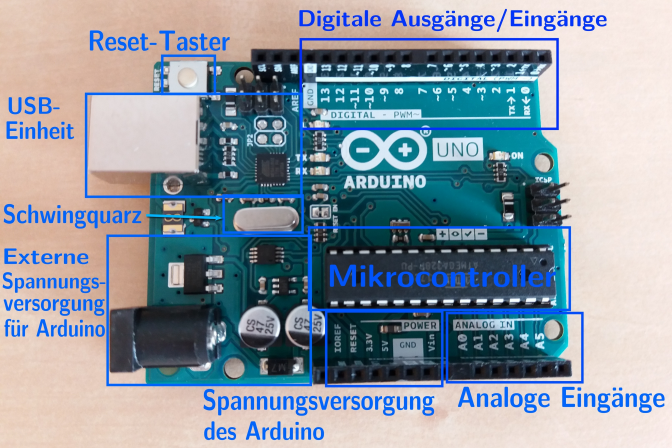
\includegraphics[width=0.8\textwidth]{pics/arduino-beschriftet.png}
	\caption{Die wichtigsten Komponenten eines Arduino Uno.}
	\label{abb:arduino-beschriftet}
\end{figure}

Abbildung \ref{abb:arduino-beschriftet} zeigt die wichtigsten Komponenten des Arduino Uno. Eine genauere Beschreibung dieser Funktionseinheiten und ihrer spezifischen Eigenschaften findet sich in Anhang \ref{sec:ueberblick}. Wichtig sind an dieser Stelle vor allem folgende Punkte:
\begin{itemize}
	\item Über den USB-Anschluss und das mitgelieferte Kabel lässt sich der Arduino mit dem PC verbinden und programmieren.
	\item Das Programm läuft nach dem Übertragen auf dem eigentlichen Mikrocontroller, dem langen schwarzen Ding in der Mitte. Der ganze Rest auf dieser kleinen Platine dient der einfacheren Handhabung des Mikrocontrollers.
	\item An den Seiten befinden sich die Pin-Leisten, an die sich zum Beispiel LEDs anschließen lassen. Die Pins sind durchnummeriert, sodass sie im Programm angesprochen werden können. \emph{GND} steht für \enquote{Ground} oder den Minus-Kontakt. \emph{5V} steht für den Plus-Kontakt und gibt an, dass dort stets eine Spannung von 5V anliegt, wenn der Arduino über USB oder Batterie mit Strom versorgt wird. Die durchnummerierten Digitalpins können durch das Programm ebenfalls auf 5V gesetzt werden (\texttt{HIGH}), aber auch auf 0V, sodass kein Strom fließt (\texttt{LOW}).
\end{itemize}
\vfill

\section{Das Open Roberta Lab und Nepo4Arduino}

Nepo4Arduino ist eine graphische Programmiersprache, die vom Fraunhofer Institut für Intelligente Analyse- und Informationssysteme im Rahmen des Open Roberta Labs für verschiedene Robotersysteme entwickelt wird. Durch die bereit gestellten Blöcke wird der Einstieg in die Programmierung des Arduino sehr einfach gemacht. Gleichzeitig lassen sich aber auch sehr komplexe Programme entwickeln und man kann jederzeit das textbasierte Programm in der Sprache C++ einsehen.

Um den Arduino zu programmieren, ruft man die Adresse \url{https://lab.open-roberta.org/} auf und wählt dann $\infty$ \texttt{Nepo4Arduino} und im nächsten Schritt den Arduino Uno aus. Damit das dort erstellte Programm aus dem Browser auf den Arduino übertragen werden kann, muss außerdem der \texttt{Open Roberta Connector} installiert werden. Auf der \href{https://jira.iais.fraunhofer.de/wiki/display/ORInfo/Open+Roberta+Wiki}{Wiki-Seite} gibt es eine \href{https://jira.iais.fraunhofer.de/wiki/display/ORInfo/Open+Roberta+Connector}{Installations-Anleitung} und eine \href{https://jira.iais.fraunhofer.de/wiki/display/ORInfo/Vorbereitung+Nepo4Arduino}{Anleitung zum Verbinden des Arduino mit dem Open Roberta Lab}.

Abbildung \ref{abb:openrobertalab} zeigt eine Übersicht über die Oberfläche des Open Roberta Lab, jedoch lernt man sie am besten kennen, indem man einfach drauf loslegt und ausprobiert, was sich damit anstellen lässt.

\begin{figure}[H]
	\centering
	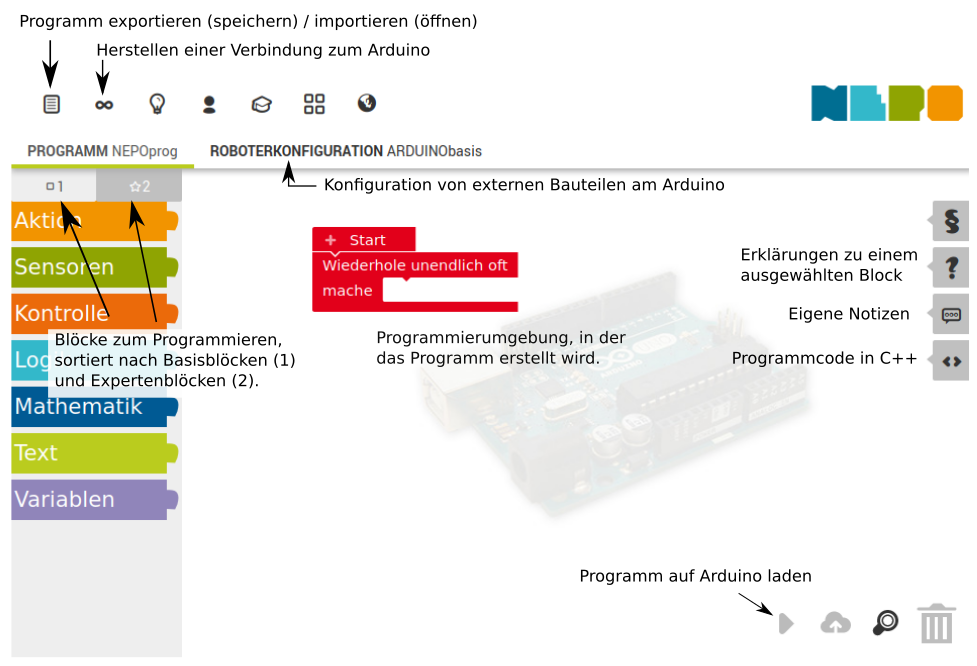
\includegraphics[width=\textwidth]{./pics/openrobertalab.png}
	\caption{Übersicht über die Funktionen von Open Roberta Lab.}
	\label{abb:openrobertalab}
\end{figure}

\newpage
\section{Digitale Ausgänge steuern}

\begin{ziel}
	\textbf{Ziel:} Es soll das erste Testprogramm auf den Arduino übertragen werden, mit dem man üblicherweise überprüft, ob der Arduino (oder ein anderer Mikrocontroller) richtig funktioniert.
\end{ziel}

\begin{aufgabe} \emph{Test der Funktionsweise}
	
	Zum Testen der Funktionsweise soll die bordeigene LED zum Blinken gebracht werden:
	\begin{itemize}[itemsep=0ex]
		\item Stelle LED an.
		\item Warte eine Sekunde.
		\item Stelle LED aus.
		\item Warte eine Sekunde.
	\end{itemize}
	
	\begin{enumerate}[label= \alph*), itemsep=0ex, parsep=0ex]
		\item Verbinde den Arduino mit dem Open Roberta Lab nach der \href{https://jira.iais.fraunhofer.de/wiki/display/ORInfo/Vorbereitung+Nepo4Arduino}{Anleitung zum Verbinden des Arduino}.
		\item Überprüfe zunächst in der Roboterkonfiguration, ob der Block für die Board-LED bereits eingestellt ist. Benenne die LED als \enquote{BoardLED}.
		\item Erstelle das oben formulierte Programm mit Nepo4Arduino und übertrage es auf den Arduino.
		\item Zum Speichern des Programms wähle im ~\nepomenu\texttt{Menü} die Funktion ~\nepoexport\texttt{exportiere Programm}. Finde das Programm im Download-Ordner deines Computers und benenne es als \texttt{Blink.xml}. Speichere es dann an einem sinnvollen Ort ab.
		
		\emph{Hinweis:} Du kannst das Programm im gleichen Menü wieder importieren, um es zu einem späteren Zeitpunkt wieder aufzurufen.
	\end{enumerate}
\end{aufgabe}

\begin{zsfg}{{Algorithmus, Anweisung und Argument}}
	\begin{wrapfigure}{r}{0.3\textwidth}
		\centering
		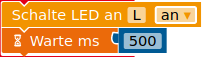
\includegraphics[width=0.3\textwidth]{./pics/anweisungen-bsp.png}
		\caption{Anweisungen und Argumente in einem Algorithmus.}
		\label{abb:befehlbsp}
	\end{wrapfigure}
	Ein Programm besteht aus einer Folge von Anweisungen. Man spricht auch von Algorithmen: Ein Algorithmus ist eine eindeutige Handlungsvorschrift zur Lösung eines Problems, die aus endlich vielen Anweisungen besteht (s. \href{https://de.wikipedia.org/wiki/Algorithmus}{Wikipedia}).
	
	Eine Anweisung \emph{kann} ein oder mehrere \emph{Argumente} haben, die zum Beispiel festlegen, welche LED geschaltet oder wie lange gewartet werden soll.
\end{zsfg}

\begin{aufgabe}
	Wir nutzen in den ersten Kapiteln sehr häufig LEDs, weil sich die Grundlagen mit ihnen einfach erarbeiten lassen, aber auch weil sie eine enorme Bedeutung in der heutigen Welt haben. Notiere dir zur Verdeutlichung eine Woche lang alle Geräte, die dir begegnen oder die dir einfallen, in denen LEDs verbaut sind.
\end{aufgabe}
\vfill

\newpage
\section{Aufbau von Schaltungen auf der Steckplatine}

In der Regel braucht man für interessante Geräte zusätzliche \emph{Hardware} (Sensoren, Motoren, \dots), die am Arduino angeschlossen wird. Bevor diese fest verlötet werden, nutzt man normalerweise Steckverbindungen bzw. baut die Schaltung auf einem kleinen Steckbrett auf, auf dem man die Verbindungen schnell wieder lösen kann, falls nötig. Steckbretter sind aus dem Physikunterricht bekannt. Abbildung \ref{abb:steckbrett} zeigt, welche Kontakte auf dem Steckbrett miteinander verbunden sind.

\begin{figure}[H]
	\centering
	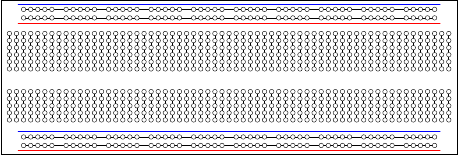
\includegraphics[width=0.8\textwidth]{./Zeichnungen/steckbrett.png}
	\caption{Die Steckverbindungen sind außen in Längsrichtung und innen in Querrichtung miteinander verbunden.}
	\label{abb:steckbrett}
\end{figure}

\begin{ziel}
	\textbf{Ziel:} Eine externe LED an Pin 13 soll zum Leuchten gebracht werden. Diese kann genutzt werden, um das Blinken einer Alarmanlagen-LED zu simulieren.
\end{ziel}

\medskip
\begin{minipage}{0.48\textwidth}
	\begin{figure}[H]
		\centering
		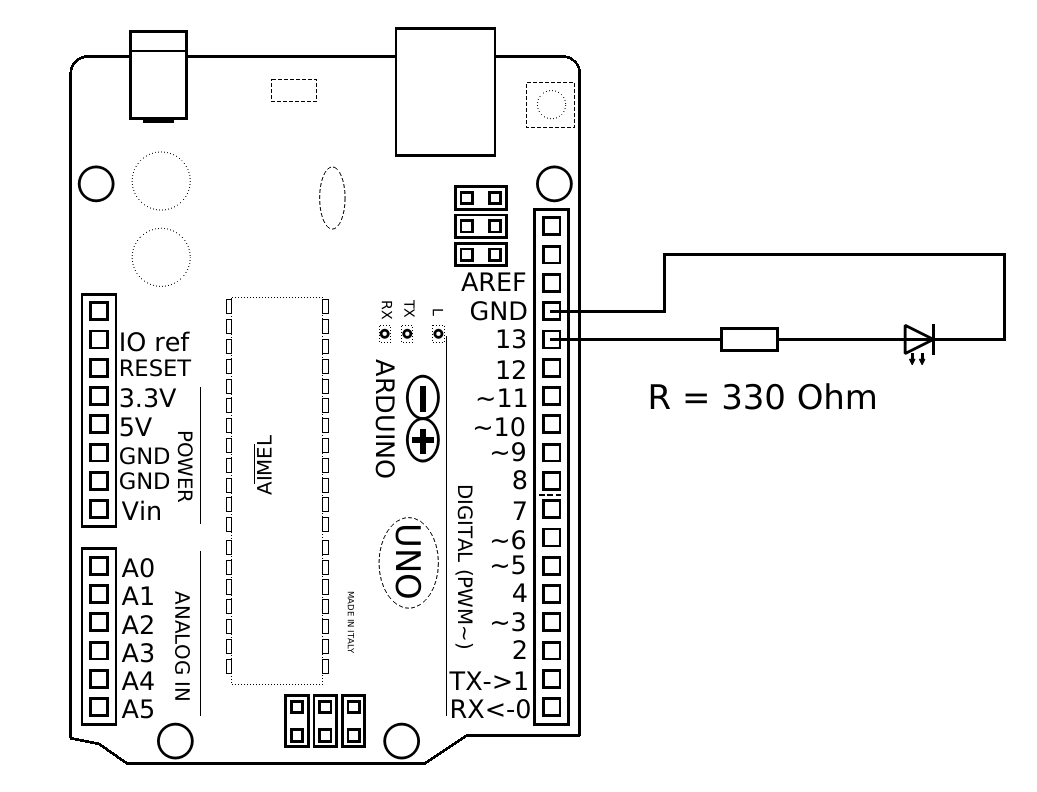
\includegraphics[width=\textwidth]{./Zeichnungen/Schaltplan-LED.png}
		\caption{Schaltplan zum Anschließen einer LED mit Vorwiderstand an Pin 13.}
	\end{figure}
\end{minipage}
\hfill
\begin{minipage}{0.5\textwidth}
	\emph{Hinweise:} 
	
	Es kann das Programm aus dem vorherigen Abschnitt wieder verwendet werden, da die Board-LED ebenfalls mit Pin 13 verbunden ist. Allerdings gibt es noch etwas zu beachten: Wenn die LED an Pin 13 angeschaltet wird, bedeutet das, dass der Arduino an Pin 13 eine Spannung von 5V (Pluspol) gegenüber GND (Minuspol) ausgibt. Die LED verträgt jedoch nur (je nach Farbe) gut 2\,V. Daher ist die LED mit einem Vorwiderstand von $\SI{330}{\SIUnitSymbolOhm}$ verbunden.
	
	Die LED ist ein sogenanntes gepoltes Bauteil. Das heißt, dass der lange Kontaktstift der LED an den Pluspol angeschlossen werden \emph{muss} und der kurze an den Minuspol (GND) angeschlossen werden \emph{muss}.
\end{minipage}
\marginpar{%
	\begin{tikzpicture}[rotate=-90, scale=0.16, baseline=-1mm]
	\shade [left color=lightgray, right color=gray] (-5,0.8) rectangle (10,1.2);
	\shade [left color=LightSkyBlue, right color=NavyBlue] (0,0) -- (5,0) arc [start angle=-135, end angle=135, radius=1.414] -- (0,2) arc [start angle=45, end angle=315, radius=1.414];
	\fill [orange] (0,0) rectangle ++(0.5,2);
	\fill [orange] (1,0) rectangle ++(0.5,2);
	\fill [black] (2,0) rectangle ++(0.5,2);
	\fill [black] (3,0) rectangle ++(0.5,2);
	\fill [brown] (4.5,0) rectangle ++(0.5,2);
	\end{tikzpicture}
	\\
	
	\tiny 330 Ohm
	
	Widerstand
	\\
	\\
	\begin{tikzpicture}[]
	\fill [CadetBlue!70!green] (0,0) circle (0.25cm); %ursprünglich gray!50!white
	\fill [CadetBlue!70!green] (-0.25,0) rectangle (0.25,-0.3);
	\draw [ultra thick, gray!50!white] (-0.1,-0.3) -- (-0.1,-0.8) node [left, black] {\sffamily -};
	\draw [ultra thick, gray!50!white] (0.1,-0.3) -- (0.1,-1) node [right, black] {\sffamily +};
	\end{tikzpicture}
	
	\tiny LED
}

\bigskip
\begin{projekt}[Ampel]\label{proj:ampel}
	Baue und programmiere eine Ampelschaltung! Verwende für die LEDs aussagekräftige Namen. Denke daran, dein Programm abzuspeichern!
	
	\emph{Für Schnelle:} Erweitere die Ampel um einen Nachtmodus.
\end{projekt}

%\bigskip
\begin{projekt}[Augentestgerät]\label{proj:augentest}
	Moderne Fernseher nutzen meist eine Bildwiederholungsrate von 144 Hertz; das bedeutet, es werden 144 Bilder pro Sekunde eingespielt. Finde mithilfe des Blink-Programms heraus, ab welchem Blinkintervall du kein Flackern mehr wahrnimmst und berechne, wie viele \enquote{Bilder} pro Sekunde sich daraus ergeben. Vergleiche diesen Wert mit der Bildwiederholungsrate im Fernsehen.
	
	{\scriptsize Idee: Frick, Fritsch und Trick (2015): \emph{Einführung in Mikrocontroller - Der Arduino als Steuerzentrale}, Bad Saulgau}
\end{projekt}

\begin{zsfg}{LED}
%	\begin{wrapfigure}{r}{0.3\textwidth}
%		\centering
%		\vspace{-0.5\baselineskip}
%		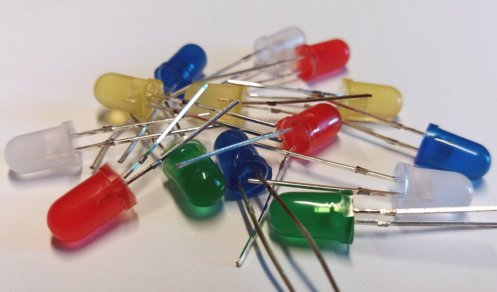
\includegraphics[width=0.3\textwidth]{./pics/led-sammlung.jpg}
%		\label{abb:led-sammlung}
%		\vspace{-\baselineskip}
%	\end{wrapfigure}
	\begin{minipage}{0.7\textwidth}
		Die Bezeichnung \enquote{LED} steht für \emph{Licht emittierende Diode} (kurz: Leuchtdiode). Sie ist ein Halbleiterbauelement, das elektrische Energie sehr effizient in Lichtenergie umwandelt und daher heute weite Verbreitung in allen Bereichen gefunden hat, in denen Licht benötigt wird. Sie ist ein gepoltes Bauteil. Das heißt, dass der lange Kontaktstift der LED mit dem Pluspol und der kurze Kontaktstift mit dem Minuspol verbunden werden muss, damit sie leuchten kann. Damit die LED nicht durchbrennt, muss in der Regel ein Vorwiderstand angebracht werden, um sie zu betreiben.
	\end{minipage}
	\hfill
	\begin{minipage}{0.28\textwidth}
%		\begin{minipage}{0.48\textwidth}
%			\centering
%			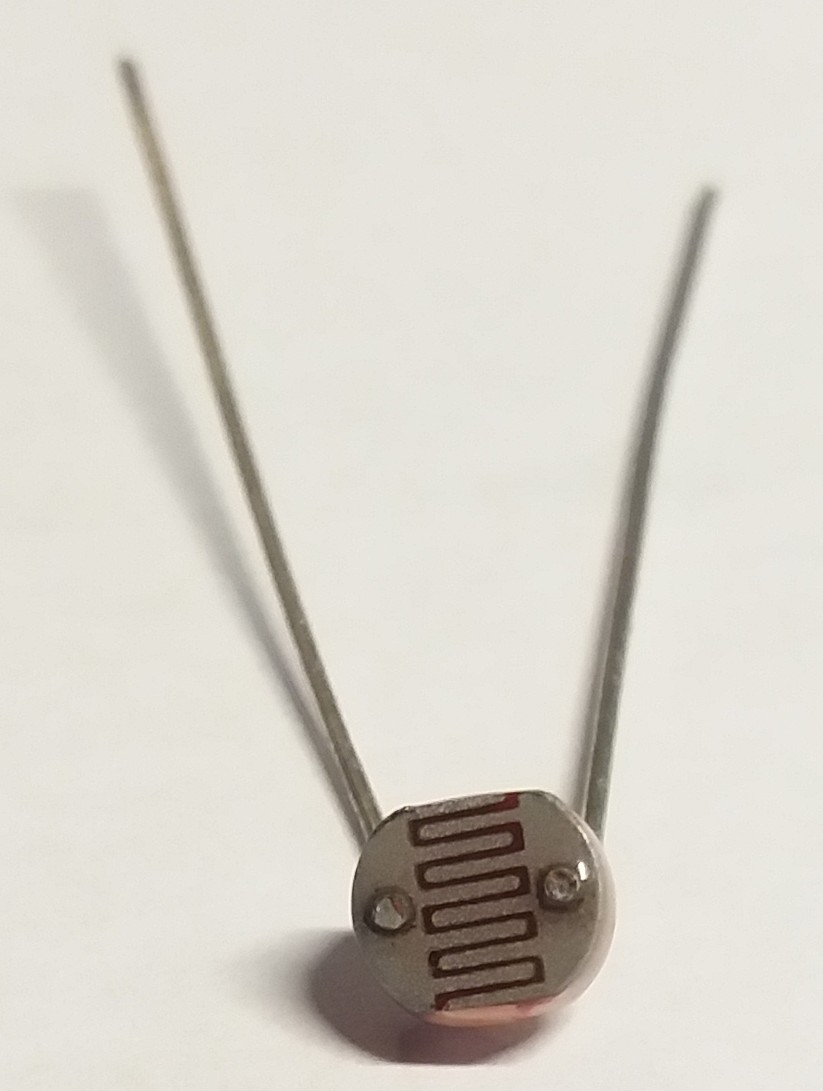
\includegraphics[width=0.9\textwidth]{./pics/ldr.jpg}
%		\end{minipage}
%		\hfill
%		\begin{minipage}{0.48\textwidth}
%			\centering
%			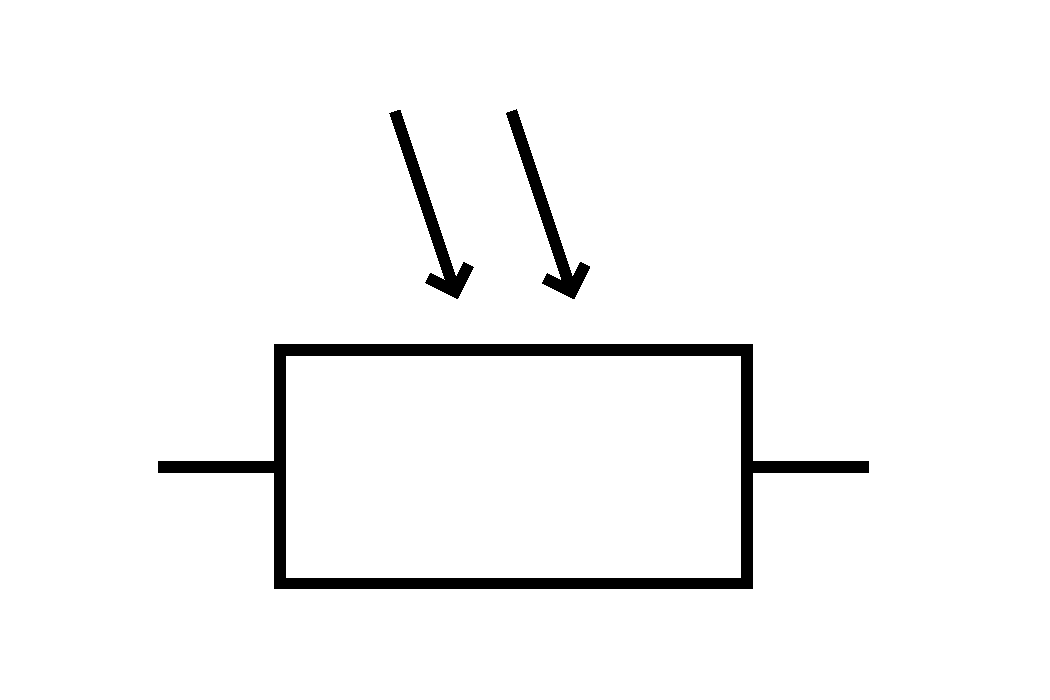
\includegraphics[width=\textwidth]{./pics/ldr-schaltsymbol.png}
%		\end{minipage}
		\centering
%		\vspace{-0.5\baselineskip}
		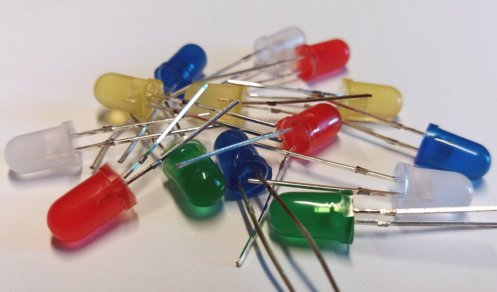
\includegraphics[width=\textwidth]{./pics/led-sammlung.jpg}
%		\label{abb:led-sammlung}
		
		\bigskip
		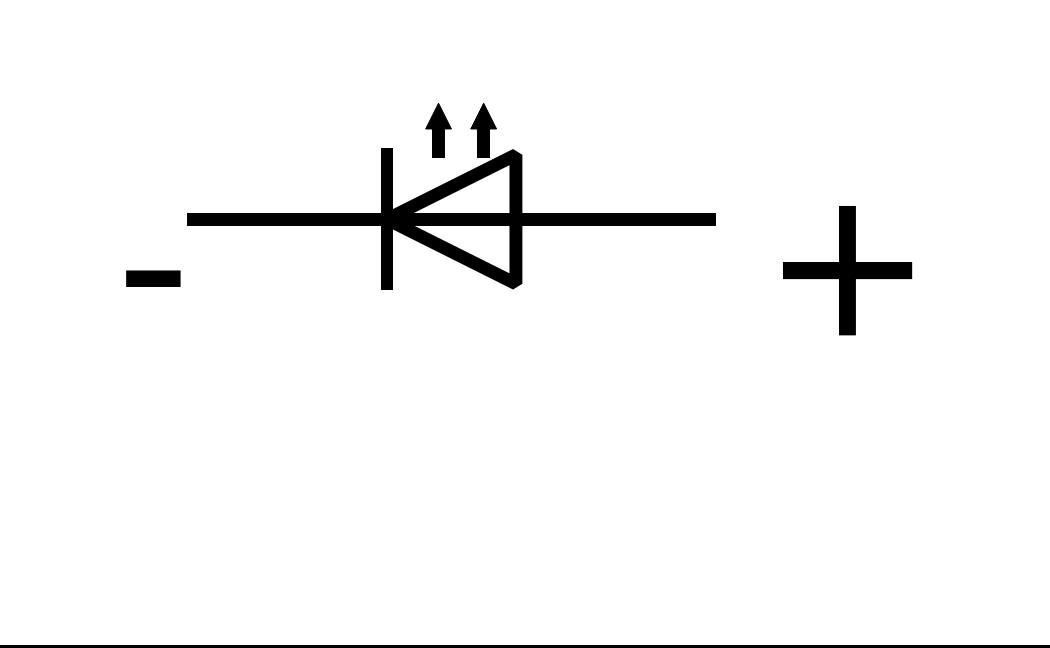
\includegraphics[width=0.7\textwidth]{./Zeichnungen/led-schaltsymbol.png}
	\end{minipage}
\end{zsfg}

\section{Widerstandsringe ablesen}
\label{sec:widerstandsringe}

Leider sind die Widerstände zu klein, um ihren Wert darauf gut lesbar zu drucken. Daher werden die Widerstände mit Ringen versehen, aus deren Farbe sich die Größe des Widerstands ablesen lässt. Um im Folgenden jeweils den passenden Widerstand aus dem Bausatz auswählen zu können, müssen wir diesen Farbcode lesen können.

Bei den blauen Kohleschichtwiderständen, die wir verwenden, gibt es fünf Ringe und jede Ringfarbe steht für eine Zahl. Die ersten drei Ringe bilden die ersten drei Ziffern des Widerstandswertes ab. Die darauf folgende Ringfarbe steht für die Zehnerpotenz, die mit den drei Ziffern multipliziert werden muss. Dies dient dazu, auch größere Widerstandswerte codieren zu können. Der letzte Ring wiederum soll einen etwas größeren Abstand haben und steht für die Fehlertoleranz des Widerstandswertes. In der Praxis lässt sich allerdings nicht immer gut erkennen, welcher Ring der letzte und welcher der erste ist\dots

\begin{figure}[H]
	\centering
	\begin{tikzpicture}[scale=0.35]
	\shade [top color=lightgray, bottom color=gray] (-5,0.8) rectangle (10,1.2);
	\shade [top color=LightSkyBlue, bottom color=NavyBlue] (0,0) -- (5,0) arc [start angle=-135, end angle=135, radius=1.414] -- (0,2) arc [start angle=45, end angle=315, radius=1.414];
	\draw [fill=orange] (0,0) rectangle ++(0.5,2) ++(-0.25,-1) -- ++(0,-1.25) [anchor =north] node {\Large 3};
	\draw [fill=green] (1,0) rectangle ++(0.5,2) ++(-0.25,-1) -- ++(0,-1.25) [anchor =north] node {\Large 5};
	\draw [fill=black] (2,0) rectangle ++(0.5,2) ++(-0.25,-1) -- ++(0,-1.25) [anchor =north] node {\Large 0};
	\draw [fill=black] (3,0) rectangle ++(0.5,2) ++(-0.25,-1) -- ++(0.5,-1.25) [anchor =north] node {\Large $\times 1$};
	\draw [fill=brown] (4.5,0) rectangle ++(0.5,2) ++(-0.25,-1) -- ++(1.5,-1.8) [anchor =north] node {\Large $\pm1\%$};
	\end{tikzpicture}
\end{figure}
Ein Beispiel: Die Ringfarben lauten orange - grün - schwarz - schwarz - braun. Anhand der folgenden Tabelle lässt sich daraus der Wert konstruieren: $3 - 5 - 0 - \cdot 1 (=10^0) - \pm 1\% $, kurz: $\SI{350}{\SIUnitSymbolOhm}\pm\SI{3,5}{\SIUnitSymbolOhm}$.

\begin{table}[H]
	\centering
	%\rowcolors{1}{lightgray}{white}
	\begin{minipage}[c]{\textwidth}
		\begin{tabu} to \textwidth {X[L,2]X[C]X[C]X[C]X[C,3]X[C,2]}
			\toprule
			\textbf{Ringfarbe} & \textbf{1. Ring} & \textbf{2. Ring} & \textbf{3. Ring} & \textbf{4. Ring (Multiplikator)} & \textbf{5. Ring (Toleranz)} \\
			\midrule
			\textcolor{black}{\rule{1cm}{0.4cm}} Schwarz & 0 & 0  & 0 & $\times 1$ / $\times 10^0$ & - \\
			\textcolor{brown}{\rule{1cm}{0.4cm}} Braun   & 1 & 1 & 1& $\times10$ / $\times 10^1$ & 1\% \\
			\textcolor{red}{\rule{1cm}{0.4cm}} Rot  & 2 & 2 & 2& $\times100$ / $\times 10^2$ & 2\% \\
			\textcolor{orange}{\rule{1cm}{0.4cm}} Orange & 3 & 3 & 3& $\times 1000$ / $\times 10^3$ & - \\
			\textcolor{yellow}{\rule{1cm}{0.4cm}} Gelb & 4 & 4 & 4& $\times 10.000$ / $\times 10^4$ & - \\
			\textcolor{green}{\rule{1cm}{0.4cm}} Grün  & 5 & 5 & 5& $\times 100.000$ / $\times 10^5$ & - \\
			\textcolor{blue}{\rule{1cm}{0.4cm}} Blau  & 6 & 6 & 6& $\times 1.000.000$ / $\times 10^6$ & - \\
			\textcolor{violet}{\rule{1cm}{0.4cm}} Lila & 7 & 7 & 7& - & - \\
			\textcolor{gray}{\rule{1cm}{0.4cm}} Grau   & 8 & 8 & 8& - & - \\
			\tikz \draw (0,0) rectangle (1,0.4); Weiß & 9 & 9 & 9& - & - \\
			\textcolor{Gold}{\rule{1cm}{0.4cm}} Gold & - & - & -& $\times 0.1$ / $\times 10^{-1}$ & 5\% \\
			\textcolor{lightgray}{\rule{1cm}{0.4cm}} Silber & - & - & -& $\times 0.01$ / $\times 10^{-2}$ & 10\% \\
			\bottomrule
		\end{tabu}
	\end{minipage}
	\caption{Tabelle zur Codierung der Widerstandswerte durch Farbringe.}
	\label{tab:farbcodierung}
\end{table}

\begin{aufgabe} \emph{Erste Übung}
	
	Gib die Farbcodierung für einen Widerstand mit den folgenden Werten an:
	\begin{multicols}{2}
		\begin{enumerate}[label=\alph*),itemsep=0ex]
			\item $\SI{435}{\SIUnitSymbolOhm} (\pm 2\%)$,
			\item $\SI{570}{\kilo\SIUnitSymbolOhm} (\pm 5\%)$.
		\end{enumerate}
	\end{multicols}
\end{aufgabe}

\begin{aufgabe} \emph{Praxistest}
	\begin{enumerate}[label=\alph*), itemsep=0ex, parsep=0ex]
		\item Die Abbildung im Infokasten unten zeigt die vier wichtigsten Widerstände, mit denen wir zu tun haben werden. Bestimme die jeweilige Größe der Widerstände.
		\item Thorsten hat die Ringe eines Widerstands abgelesen: Silber - rot - lila - lila - grün. Bestimme die Größe des Widerstands.
	\end{enumerate}
	\medskip
	\emph{Zur Kontrolle:} \url{https://www.elektronik-kompendium.de/sites/bau/1109051.htm}
\end{aufgabe}

\begin{zsfg}{Ohmsche Widerstände}
	\begin{minipage}{0.65\textwidth}
		Ohmsche Widerstände dienen dazu, die Stromstärke zu begrenzen. Je größer ihr Widerstand ist, desto geringer wird die Stromstärke, wenn die Spannung gleich bleibt. Die Größe eines Widerstands lässt sich an seinen Ringen ablesen. Sie bleibt immer gleich groß.
	\end{minipage}
	\hfill
	\begin{minipage}{0.33\textwidth}
		\begin{minipage}{0.55\textwidth}
			\centering
			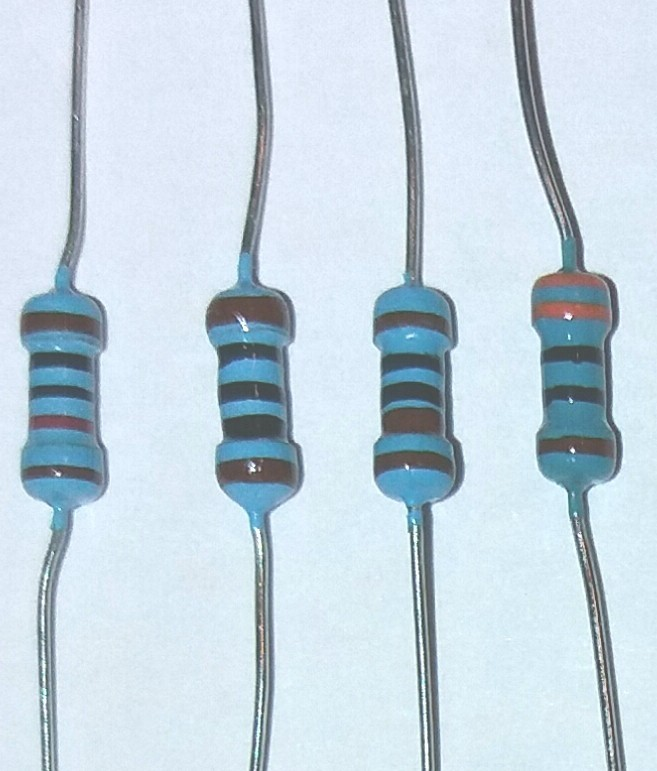
\includegraphics[width=0.9\textwidth,angle=90]{./pics/Widerstaende.jpg}
		\end{minipage}
		\hfill
		\begin{minipage}{0.43\textwidth}
			\centering
			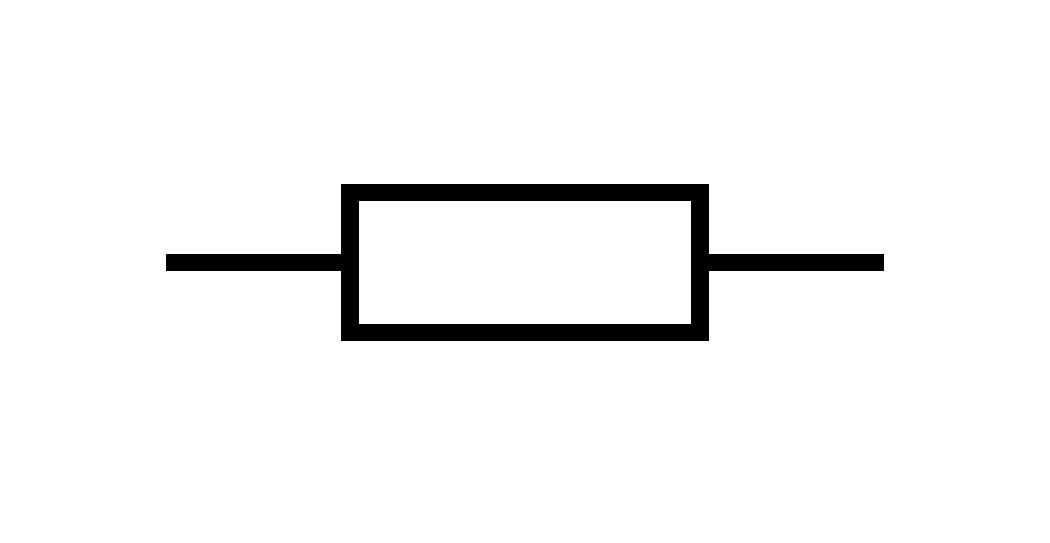
\includegraphics[width=0.8\textwidth]{./Zeichnungen/widerstand-schaltsymbol.png}
		\end{minipage}
	\end{minipage}
\end{zsfg}


\newpage
\section{Vermischte Übungen}

% TODO: Vermischte Übungen ergänzen

\begin{aufgabe} \emph{Farbcodierung von Widerständen}
	
	\begin{enumerate}[label=\alph*), itemsep=0ex]
		\item Gib die Farbcodierung der folgenden Widerstandsgrößen an:
		\begin{multicols}{3}
			\begin{enumerate}[label=(\arabic*)]
				\item $\SI{330}{\ohm} \pm 1\%$,
				\item $\SI{10}{\kilo\ohm} \pm 2\%$,
				\item $\SI{4,7}{\kilo\ohm} \pm 10\%$.
			\end{enumerate}
		\end{multicols}
		\item Gib die Größe der folgenden Widerstände an:
		\begin{multicols}{2}
			\begin{enumerate}[label=(\arabic*)]
				\item \begin{tikzpicture}[scale=0.3]
				\shade [top color=lightgray, bottom color=gray] (-5,0.8) rectangle (10,1.2);
				\shade [top color=LightSkyBlue, bottom color=NavyBlue] (0,0) -- (5,0) arc [start angle=-135, end angle=135, radius=1.414] -- (0,2) arc [start angle=45, end angle=315, radius=1.414];
				\draw [fill=red] (0,0) rectangle ++(0.5,2);
				\draw [fill=red] (1,0) rectangle ++(0.5,2);
				\draw [fill=black] (2,0) rectangle ++(0.5,2);
				\draw [fill=black] (3,0) rectangle ++(0.5,2);
				\draw [fill=brown] (4.5,0) rectangle ++(0.5,2);
				\end{tikzpicture}
				\item \begin{tikzpicture}[scale=0.3]
				\shade [top color=lightgray, bottom color=gray] (-5,0.8) rectangle (10,1.2);
				\shade [top color=LightSkyBlue, bottom color=NavyBlue] (0,0) -- (5,0) arc [start angle=-135, end angle=135, radius=1.414] -- (0,2) arc [start angle=45, end angle=315, radius=1.414];
				\draw [fill=green] (0,0) rectangle ++(0.5,2);
				\draw [fill=blue] (1,0) rectangle ++(0.5,2);
				\draw [fill=black] (2,0) rectangle ++(0.5,2);
				\draw [fill=yellow] (3,0) rectangle ++(0.5,2);
				\draw [fill=lightgray] (4.5,0) rectangle ++(0.5,2);
				\end{tikzpicture}
			\end{enumerate}
		\end{multicols}
	\end{enumerate}
	\emph{Hinweis:} Als Hilfsmittel ist die Widerstandskarte aus den Boxen zugelassen.
\end{aufgabe}


\vfill


\begin{links}
	\item \href{https://www.youtube.com/watch?v=EbVmfGNwn0g}{FUTUREMAG}
	
	Kurze Dokumentation des FUTUREMAG zur Arduino-Welt
	
	\item \href{https://www.heise.de/make/meldung/Mehr-Komfort-der-Arduino-Ueberkopfwecker-4046184.html}{Arduino-Wecker}
	
	Mit einem selbst gebauten Wecker, der Uhrzeit und Alarmzeit getrennt voneinander anzeigt, erfüllte ein Bastler seinen Wunsch nach mehr Komfort.
	
	\item \href{https://www.instructables.com/id/Aquarium-LED-Controller/}{Aquarium-Licht}
	
	Der Bastler hinter diesem Projekt wollte seinen Fischen im Aquarium ein natürliches Licht einschließlich Sonnenaufgang, Sonnenuntergang und Nacht gönnen. Auf die gleiche Art und Weise kann man natürlich auch sein Terrarium beleuchten.
	
	\item \href{https://www.heise.de/make/meldung/Kein-Geld-fuer-eine-Oculus-Rift-VR-Brille-selbstgebaut-3949507.html}{VR-Brille}
	
	Drei Schüler aus Frankreich hatten kein Geld für eine Virtual Reality Brille – aber dafür das Know How, um sich mit einem Arduino und einem Gehäuse aus dem 3D-Drucker selbst eine VR-Brille zu basteln.
\end{links}




\pagecolor{CadetBlue!70!green}
\chapter{Bausteine von Algorithmen}
\label{kap:bausteinealgorithmen}

Mit dem Arduino und einigen einfachen Bauteilen lassen sich bereits zahlreiche Projekte umsetzen. Allerdings wird die Programmierung schnell unübersichtlich oder unnötig aufwendig, wenn man sich nicht mit algorithmischen Strukturen auskennt. Daher geht es im folgenden Kapitel um die Einführung von grundlegenden algorithmischen Bausteinen.

\bigskip
In diesem Kapitel lernst du\dots
\begin{itemize}
	\item \dots Entscheidungen zu programmieren,
	\item \dots den Arduino mit dem Computer kommunizieren zu lassen,
	\item \dots zwischen unterschiedlichen Datentypen zu unterscheiden,
	\item \dots Entscheidungen anhand mehrerer Kriterien zu treffen,
	\item \dots wie man Programme zur Planung oder zum Vergleich auf Papier einfach darstellen kann
	\item \dots Variablen zu benutzen,
	\item \dots zufällige Ereignisse zu programmieren,
	\item \dots mit Schleifen effizient zu programmieren,
	\item \dots systematisch nach Fehlern im Programm zu suchen.
\end{itemize}

\bigskip

\bigskip

\begin{projektueberblick}
	\item Fußgängerampel \dotfill \pageref{proj:fussampel}
	\item Juke-Box \dotfill \pageref{proj:jukebox}
	\item Straßenlampe \dotfill \pageref{proj:strassenlampe}
	\item Carport-Lampe \dotfill \pageref{proj:carportlampe}
	\item Auto-Blinker \dotfill \pageref{proj:blinker}
	\item Bombe bauen \dotfill \pageref{proj:bombe}
	\item Reaktionszeitmesser \dotfill \pageref{proj:reaktionszeitmesser}
	\item Reaktionsspiel \dotfill \pageref{proj:reaktionsspiel}
	\item Alarmanlage mit Lichtschranke \dotfill \pageref{proj:alarmanlage}
\end{projektueberblick}

\newpage
\nopagecolor
\section{Entscheidungen programmieren}
\label{sec:entscheidungen}

Schaltungen und Programme werden erst dann richtig interessant, wenn sie auf ihre Umwelt reagieren. Im einfachsten Fall lässt sich dazu ein Taster einbauen, mit dem sich von außen entscheiden lässt, wie das Programm weiterlaufen soll. Dementsprechend müssen im Programm \emph{Fallunterscheidungen} eingebaut werden.

\begin{ziel}
	\textbf{Ziel:} Der Arduino soll auf Eingaben aus seiner Umwelt reagieren.
\end{ziel}

\bigskip
\begin{projekt}[Fußgängerampel]\label{proj:fussampel}
	\begin{wrapfigure}{r}{0.4\textwidth}
		\centering
		\vspace{-2\baselineskip}
		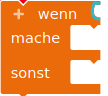
\includegraphics[width=0.15\textwidth]{./pics/wenn-mache-sonst.png}
		\label{abb:falls-dann}
	\end{wrapfigure}
	Baue und programmiere eine Fußgängerampel! Nutze dazu die Informationen aus dem Info-Kasten zum Taster.
\end{projekt}

\bigskip
\begin{zsfg}{Taster}
	\begin{minipage}{0.7\textwidth}
		Ein Taster ist wie ein Schalter, kann also geschlossen sein (Strom fließt) oder offen sein (Strom fließt nicht). Im Gegensatz zum Schalter springt ein Taster aber automatisch wieder in den offenen Zustand zurück, wenn er losgelassen wird.
	\end{minipage}
	\hfill
	\begin{minipage}{0.28\textwidth}
		\begin{minipage}{0.63\textwidth}
			\centering
			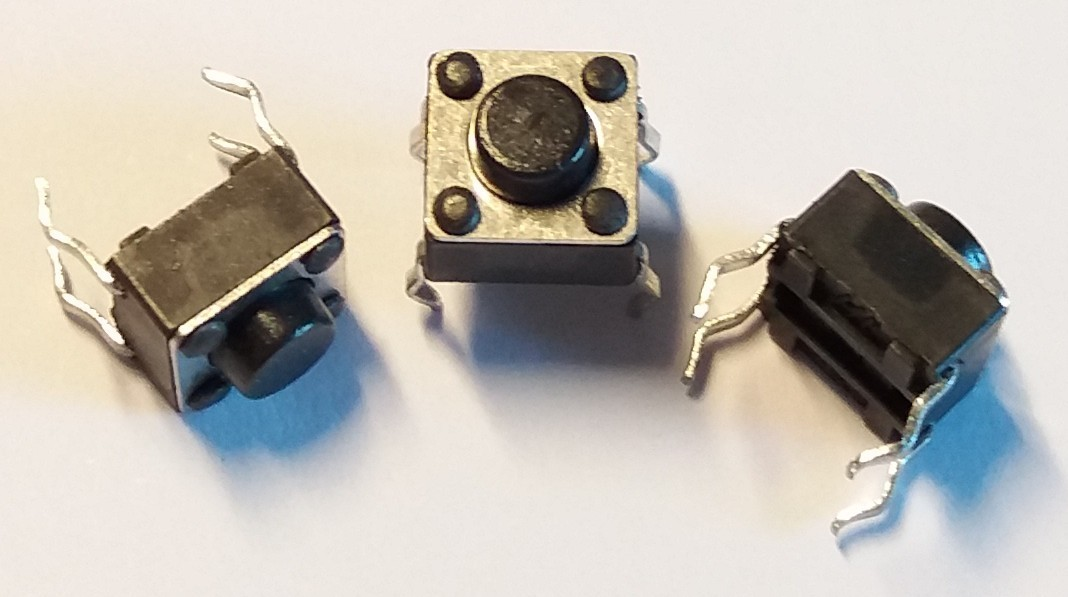
\includegraphics[width=\textwidth]{./pics/taster.jpg}
		\end{minipage}
		\hfill
		\begin{minipage}{0.33\textwidth}
			\centering
			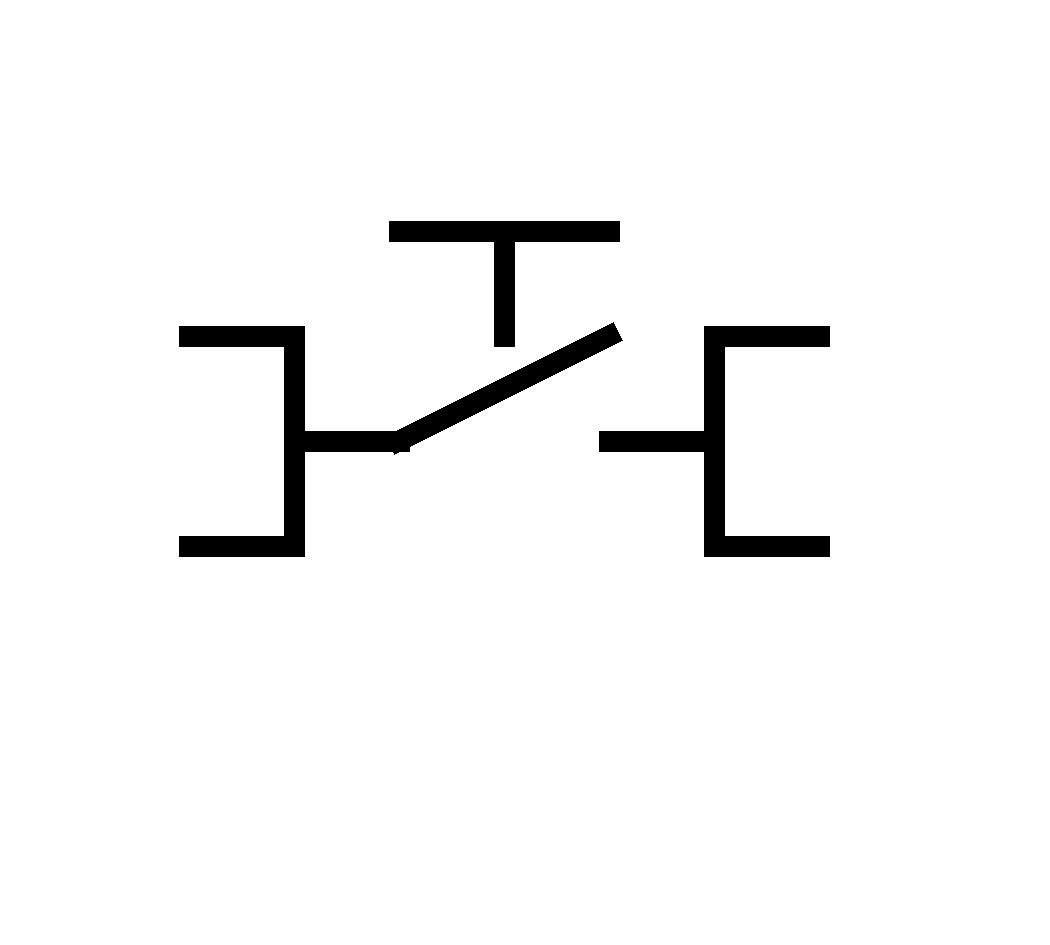
\includegraphics[width=\textwidth]{./Zeichnungen/taster-schaltsymbol.png}
		\end{minipage}
	\end{minipage}		
\end{zsfg}


\begin{minipage}{0.45\textwidth}
	In dem rechts abgebildeten Schaltplan ist dargestellt, wie man einen Taster am Arduino so anschließt, dass man seinen Zustand im digitalen Pin 3 auslesen kann. Unten ist die zugehörige Taster-Konfiguration abgebildet.
	
	\begin{figure}[H]
		\centering
		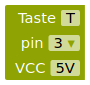
\includegraphics[width=0.3\textwidth]{./pics/tasterkonfiguration.png}
		\label{abb:tasterkonfiguration}
	\end{figure}

	\bigbreak
	\bigbreak
	\bigbreak
\end{minipage}
\hfill
\begin{minipage}{0.45\textwidth}
	\begin{figure}[H]
		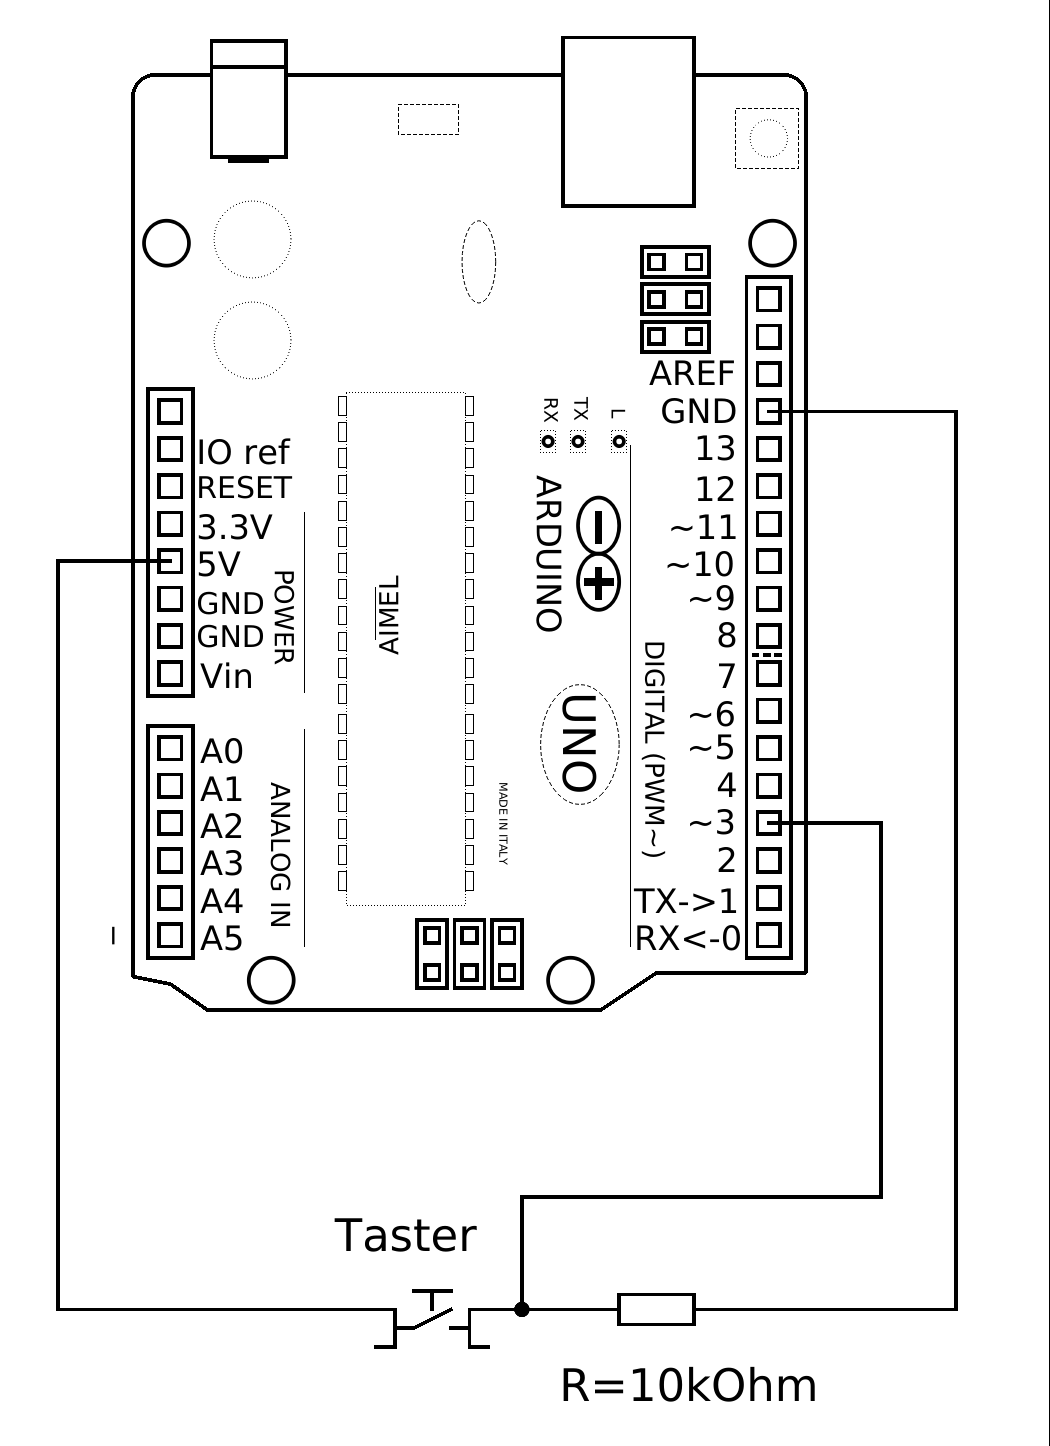
\includegraphics[width=0.8\textwidth]{./Zeichnungen/taster-an-arduino.png}
		\label{abb:schaltplan-taster}
	\end{figure}
\end{minipage}


\newpage
\begin{projekt}[Juke-Box]\label{proj:jukebox}
	\begin{wrapfigure}{r}{0.5\textwidth}
		\centering
		\vspace{-\baselineskip}
		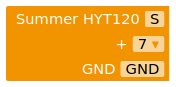
\includegraphics[width=0.25\textwidth]{pics/piezokonfiguration.png}
		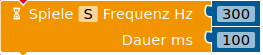
\includegraphics[width=0.35\textwidth]{pics/piezo-steuerung.png}
		\vspace{-\baselineskip}
		\label{abb:piezo-steuerung}
	\end{wrapfigure}
	Baue und programmiere eine Juke-Box!
	
	Die Juke-Box soll zwei verschiedene, kurze Melodien \emph{anspielen} können. Dazu werden zwei Taster auf die beschriebene Art an zwei digitale Pins des Arduino angeschlossen. Schließe zudem an einen Digitalpin einen Piezo-Summer an (siehe unten). 
	
	{\scriptsize Idee: Frick, Fritsch und Trick (2015): \emph{Einführung in Mikrocontroller - Der Arduino als Steuerzentrale}, Schülerforschungszentrum Bad Saulgau}
\end{projekt}

\emph{Hinweise:}

Zwei mögliche Beispiele von Melodien mit Link zu den Noten:
\begin{itemize}[itemsep=0ex, parsep=0mm]
	\item \href{https://www.lieder-archiv.de/alle\_meine\_entchen-notenblatt\_100055.html}{\enquote{Alle meine Entchen}}:
	
	\url{https://www.lieder-archiv.de/alle\_meine\_entchen-notenblatt\_100055.html},
	\item  \href{https://www.lieder-archiv.de/o\_tannenbaum-notenblatt\_200078.html}{\enquote{Oh Tannenbaum}}:
	
	\url{https://www.lieder-archiv.de/o\_tannenbaum-notenblatt\_200078.html}.
\end{itemize}

\emph{Frequenzen in Hertz zu den Noten:}

\begin{tabular}{c|c|c|c|c|c|c|c|c|c|c|c}\footnotesize
	$c^1$ & $cis^1/des^1$ & $d^1$ & $dis^1/es^1$ & $e^1$ & $f^1$ & $fis^1/ges^1$ & $g^1$ & $gis^1/as^1$ &  $a^1$ & $ais^1/b^1$ & $h^1$\\
	\hline \footnotesize
	 262 & 277 & 294 & 311 & 330 & 349 & 370 & 392 & 415 & 440 & 466 & 494\\
\end{tabular}

\medskip
\begin{zsfg}{Piezo-Summer}
	
	\begin{minipage}{0.7\textwidth}
		Mit einem Piezo-Summer lassen sich Töne erzeugen, wenn man eine Spannung anschließt. Das lange Bein muss dabei an den Pluspol (Pin) angeschlossen werden; das kurze an den Minuspol bzw. GND. Ein Vorwiderstand ist dabei nicht notwendig, hilft aber die Lautstärke zu reduzieren.
	\end{minipage}
	\hfill
	\begin{minipage}{0.28\textwidth}
		\begin{minipage}{0.48\textwidth}
			\centering
			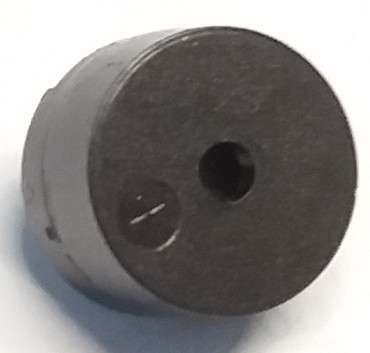
\includegraphics[width=0.9\textwidth]{./pics/piezo-summer.jpg}
		\end{minipage}
		\hfill
		\begin{minipage}{0.48\textwidth}
			\centering
			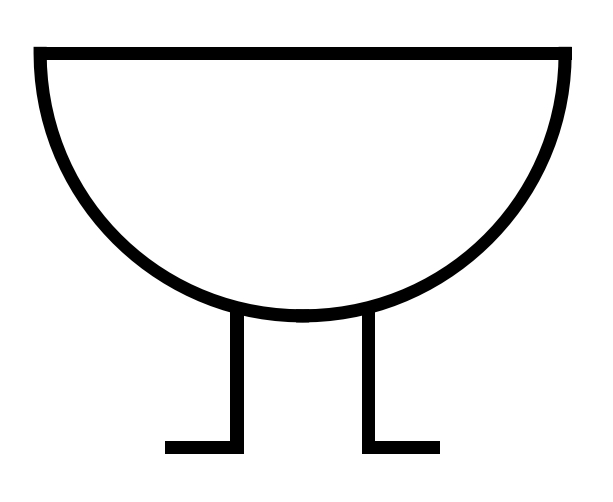
\includegraphics[width=\textwidth]{./pics/piezo-schaltsymbol.png}
		\end{minipage}
	\end{minipage}
	
	\bigskip
	\emph{Funktionsweise:}\label{piezo-effekt}
	
	\begin{wrapfigure}{r}{0.4\textwidth}
		\vspace{-\baselineskip}
		\centering
		\begin{tikzpicture}[scale=0.7]
		\fill[white] (-0.2,-0.2) rectangle (8,4);
		%Kondensator links	
		\draw[gray!40,thick] (1.5,0.2) -- ++(0,-0.3) -- ++ (1.5,0);
		\fill[gray!40] (0,0.2) rectangle (3,0.5);
		\draw[gray!40,thick] (1.5,3.5) -- ++(0,0.3) -- ++ (1.5,0);
		\fill[gray!40] (0,3.2) rectangle (3,3.5);
		% Verbindungen/Sechseck
		\draw [thick] (1.5,0.8) -- (0.59,1.32) -- (0.58,2.36) -- (1.5,2.89) -- (2.39,2.36) -- (2.39,1.32) -- (1.5,0.8);
		%Ladungsverteilung
		\node at (1.5,0.8) [circle,fill=blue!50!white, draw, inner sep=1pt] (min1) {-};
		\node at (0.58,2.36) [circle,fill=blue!50!white, draw, inner sep=1pt] (min2) {-};
		\node at (2.39,2.36) [circle,fill=blue!50!white, draw, inner sep=1pt] (min3) {-};
		\node at (1.5,2.89) [circle,fill=red!50!white, draw, inner sep=1pt] (plus1) {\tiny +};
		\node at (0.59,1.32) [circle,fill=red!50!white, draw, inner sep=1pt] (plus2) {\tiny +};
		\node at (2.39,1.32) [circle,fill=red!50!white, draw, inner sep=1pt] (plus3) {\tiny +};
		%	
		%Kondensator rechts
		\draw[thick] (5.5,0.2) -- ++(0,-0.3) -- ++ (2,0) -- ++(0,1.9) ++(-0.2,0) -- ++(0.4,0);
		\fill[blue!40] (4,0.2) rectangle (7,0.5);
		\draw[thick] (5.5,3.5) -- ++(0,0.3) -- ++ (2,0) -- ++(0,-1.9) ++(-0.3,0) -- ++(0.6,0);
		\fill[red!40] (4,3.2) rectangle (7,3.5);
		\node at (7.8,2.2) {$U$};
		% Verbindungen/Sechseck rechts
		\draw [thick] (5.5,0.8) -- (4.59,1.12) -- (4.58,2.56) -- (5.5,2.89) -- (6.39,2.56) -- (6.39,1.12) -- (5.5,0.8);
		%Ladungsverteilung rechts
		\node at (5.5,0.8) [circle,fill=blue!50!white, draw, inner sep=1pt] (min11) {-};
		\node at (4.58,2.56) [circle,fill=blue!50!white, draw, inner sep=1pt] (min21) {-};
		\node at (6.39,2.56) [circle,fill=blue!50!white, draw, inner sep=1pt] (min31) {-};
		\node at (5.5,2.89) [circle,fill=red!50!white, draw, inner sep=1pt] (plus11) {\tiny +};
		\node at (4.59,1.12) [circle,fill=red!50!white, draw, inner sep=1pt] (plus21) {\tiny +};
		\node at (6.39,1.12) [circle,fill=red!50!white, draw, inner sep=1pt] (plus31) {\tiny +};
		\end{tikzpicture}
	\end{wrapfigure}
	In einem Piezo-Summer befindet sich ein Kristall mit unterschiedlichen Ladungsschwerpunkten, der von einem Kondensator umgeben ist. Wenn von außen an den Kristall eine Spannung angelegt wird, dann verformt sich die Kristallstruktur durch die Anziehung zwischen den Ladungsschwerpunkten und den Kondensatorplatten (\emph{\href{https://de.wikipedia.org/wiki/Piezoelektrizit\%C3\%A4t}{inverser piezo-elektrischer Effekt}}). Wenn keine Spannung anliegt, verformt sich der Kristall zurück. Durch diese Verformungen entstehen Druckwellen in der Luft, die wir als Ton wahrnehmen können.
\end{zsfg}

\section{Kommunikation mit dem Arduino: Der serielle Monitor}
\label{sec:seriellermonitor}

Bisher hatte die Kommunikation mit dem Arduino stets nur eine Richtung: Vom Computer zum Arduino. Das reicht nicht mehr, wenn eine Messung vorgenommen und deren Ergebnis zurück gemeldet werden soll. Die einfachste Möglichkeit, um dies zu realisieren, ist der serielle Monitor. Dieser soll im Folgenden genutzt werden, um eine Straßenlampe zu konfigurieren, die leuchtet, wenn es dunkel wird.

\begin{ziel}
	\textbf{Frage:} Wie kann der Arduino mit dem Computer kommunizieren?
\end{ziel}

\begin{aufgabe} \emph{Test des seriellen Monitors}
	
	\vspace{-0.5\baselineskip}
	\begin{enumerate}[label=\alph*), itemsep=0ex, parsep=0mm]
		\item Implementiere ein Programm, das in jeder Sekunde \enquote{Moin!} an den seriellen Monitor sendet und übertrage es auf den Arduino.
		
		\begin{figure}[H]
			\centering
			
\includegraphics[width=0.4\textwidth]{pics/serialprint.png}
		\end{figure}
		\vspace{-0.3\baselineskip}
		\item \href{https://jira.iais.fraunhofer.de/wiki/display/ORInfo/Vorbereitung+Nepo4Arduino#VorbereitungNepo4Arduino-SerialMonitor}{Öffne den seriellen Monitor} im Open Roberta Connector mit einer Baudrate von 9600 und kontrolliere dein Programm.
	\end{enumerate}
\end{aufgabe}

\bigskip
\begin{minipage}{0.48\textwidth}
	Ein LDR ist ein Widerstand, dessen Größe von der Lichtstärke abhängt, die auf ihn trifft (siehe unten). Um ihn auslesen zu können, muss er in einem sogenannten Spannungsteiler mit einem Festwiderstand von $R_1=\SI{10}{\kilo\ohm}$ an den Arduino angeschlossen werden (siehe rechts). Der zugehörige Konfigurationsblock ist unten abgebildet.
	
	\begin{minipage}{0.48\textwidth}
		\begin{figure}[H]
			\centering
			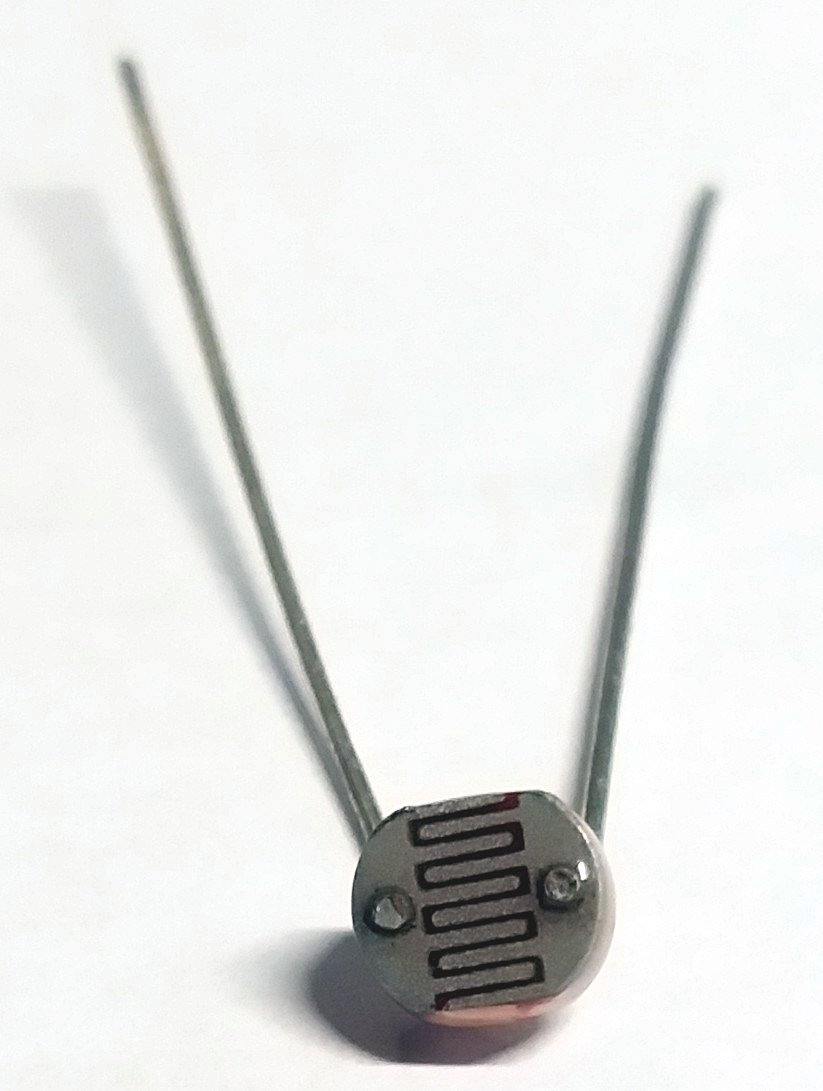
\includegraphics[width=0.5\textwidth]{./pics/ldr2.jpg}
			\caption{Ein LDR.}
		\end{figure}
	\end{minipage}
	\hfill
	\begin{minipage}{0.48\textwidth}
		\begin{figure}[H]
			\centering
			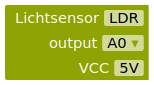
\includegraphics[width=0.9\textwidth]{./pics/ldr-konfiguration.png}
			\caption{Konfiguration des LDR.}
		\end{figure}
	\end{minipage}
\end{minipage}
\hfill
\begin{minipage}{0.48\textwidth}
	\begin{figure}[H]
		\centering
		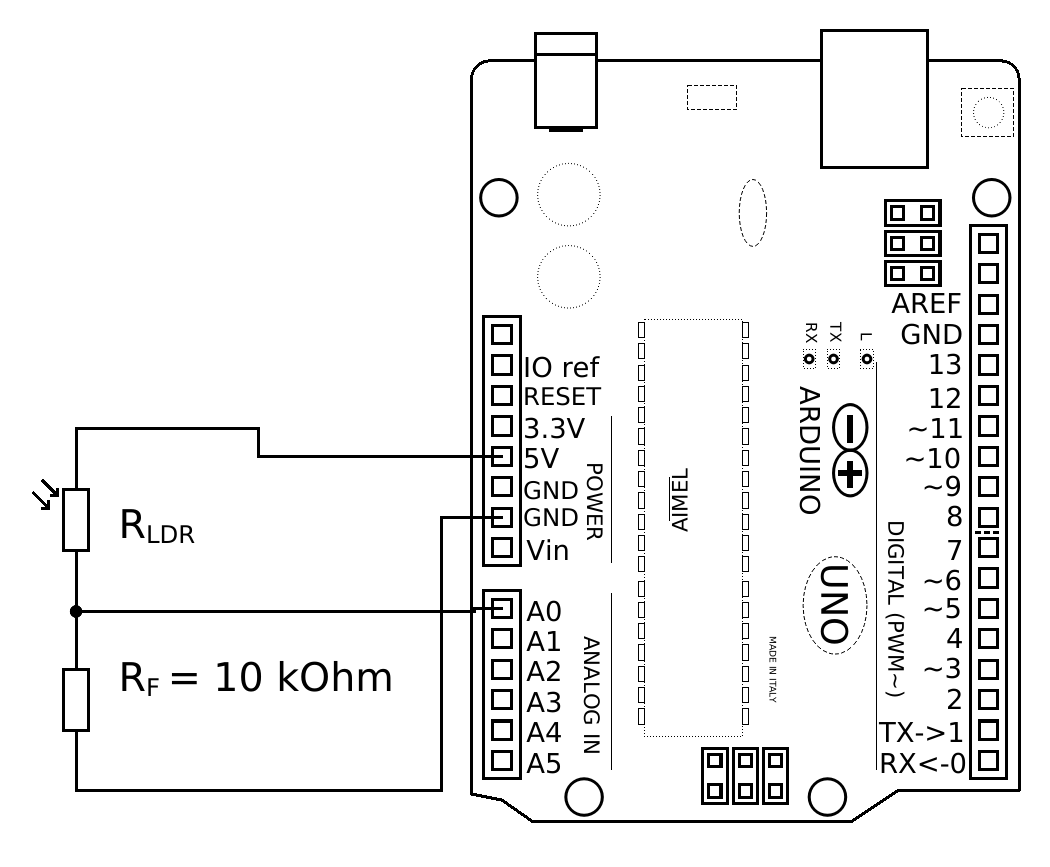
\includegraphics[width=\textwidth]{./Zeichnungen/ldr-an-arduino2.png}
		\label{abb:schaltplan-ldr}
	\end{figure}
\end{minipage}

\bigskip
\begin{aufgabe}\emph{Erste Experimente mit dem LDR}
	\vspace{-0.3\baselineskip}
	\begin{enumerate}[label=\alph*), itemsep=0ex, parsep=0mm]
		\item Baue die oben abgebildete Schaltung zum Auslesen eines LDR am Arduino auf und lasse dir die Lichtstärke in \% auf dem seriellen Monitor ausgeben.
		\item Die Veränderung der Lichtstärke in \% verläuft genau umgekehrt zur Veränderung des Widerstands des LDR. Beschreibe, wie sich der Widerstand des LDR verhält, wenn es dunkel bzw. wenn es hell wird.
	\end{enumerate}
\end{aufgabe}

\begin{projekt}[Straßenlampe]\label{proj:strassenlampe}
	Baue eine Straßenlampe, deren Licht (Vorwiderstand!) angeht, wenn es dunkel wird, und ausgeht, wenn es hell wird.
\end{projekt}

\begin{zsfg}{Fotowiderstand}
	\begin{minipage}{0.7\textwidth}
		Ein \textbf{Fotowiderstand}, kurz: \textbf{LDR} (\emph{engl. \textbf{l}ight \textbf{d}ependent \textbf{r}esistor}), ist ein lichtabhängiger Widerstand. Wenn es dunkel wird, wird der elektrische Widerstand des LDR größer; wenn es hell wird, wird der elektrische Widerstand des LDR kleiner.
	\end{minipage}
	\hfill
	\begin{minipage}{0.28\textwidth}
		\begin{minipage}{0.48\textwidth}
			\centering
			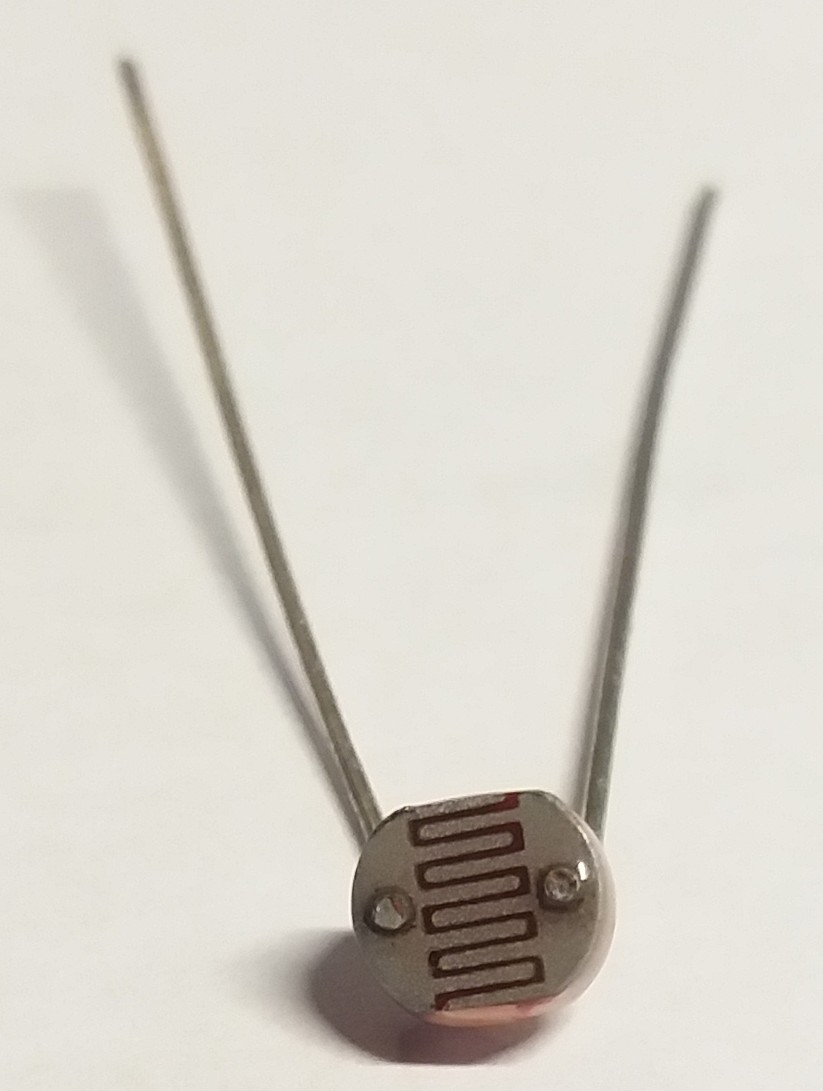
\includegraphics[width=0.9\textwidth]{./pics/ldr.jpg}
		\end{minipage}
		\hfill
		\begin{minipage}{0.48\textwidth}
			\centering
			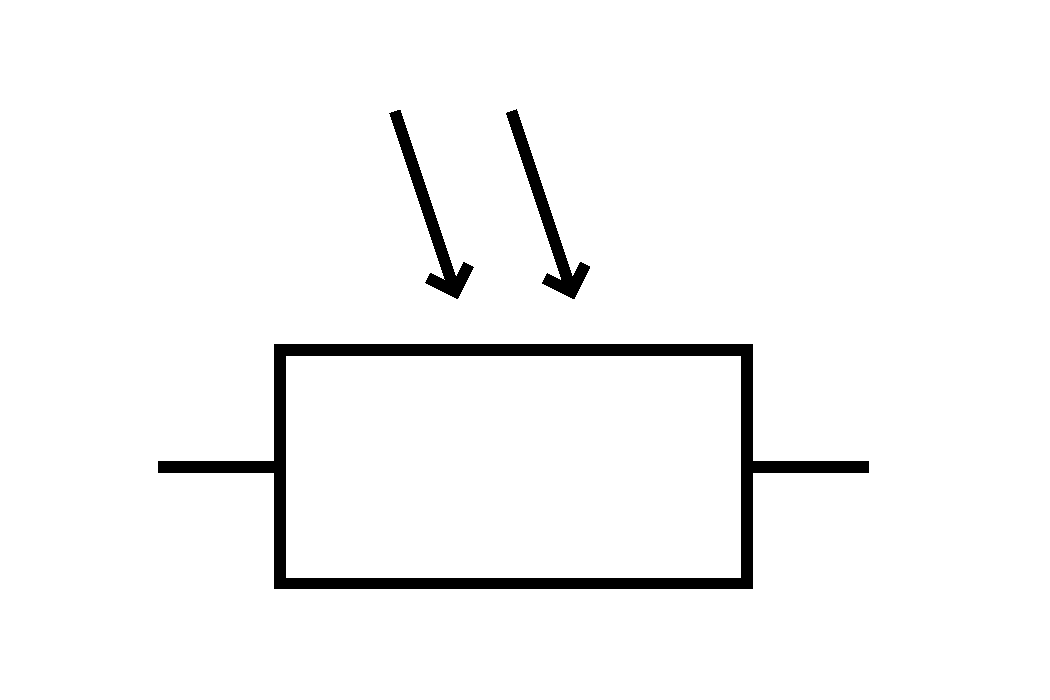
\includegraphics[width=\textwidth]{./pics/ldr-schaltsymbol.png}
		\end{minipage}
	\end{minipage}
	%	\bigskip
	%	\emph{Kurze Hintergrundinformation:}
	%	
	%	Der Fotowiderstand besteht aus einem Halbleitermaterial, in dem die Elektronen wie üblich an den Atomkern gebunden sind. Bei Halbleitern reicht jedoch schon relativ wenig Energie, um einige Elektronen so weit aus ihrer Bindung zu lösen, dass sie zum elektrischen Strom beitragen. Diese Energiezufuhr stammt von dem Licht, das auf den LDR fällt.
\end{zsfg}

\subsection{Reflexion: Datentypen}
\label{sec:datentypen}

\marginpar{%
	\textattachfile[description={Folie zu Kap. \thechapter, Datentypen}]{./Auftraege/kap3-auftrag-datentypen.pdf}{%
		\footnotesize\folie Folie %
	}%
	\footnotesize%
	\\öffnen%
}
\begin{aufgabe}
	\begin{enumerate}[label=\alph*), itemsep=0ex, parsep=0ex]
		\item In den bisherigen Anweisungen tauchten verschiedene Typen von Argumenten auf. Die Argumente sind unten noch einmal abgebildet. Gruppiere und charakterisiere sie.
		
		\bigskip
		\begin{tabu} to \textwidth {X[L]X[L,2]X[L,3]}
			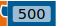
\includegraphics[width=0.1\textwidth]{./pics/zahlargument1.png} & 
			
\includegraphics[width=0.25\textwidth]{./pics/wahrheitswertargument1.png} & 
			
\includegraphics[width=0.38\textwidth]{./pics/zahlargument2.png} \\
			
\includegraphics[width=0.15\textwidth]{./pics/wahrheitswertargument2.png} & 
			
\includegraphics[width=0.2\textwidth]{./pics/textargument.png} & \\
		\end{tabu}
		\bigskip
		\item Begründe: Das Argument des \texttt{wenn}-Blocks muss hellblau sein. 
	\end{enumerate}
\end{aufgabe}

\bigskip
\begin{zsfg}{Datentypen}
	Alle Programmiersprachen unterscheiden verschiedene Datentypen, die unterschiedlich codiert sind. Die wichtigsten Datentypen in Nepo sind\dots
	\begin{itemize}
		\item 
\includegraphics[width=0.075\textwidth]{./pics/wahrheitswertargument2.png} logische Werte / Wahrheitswerte:
		
		Nur zwei Werte möglich, nämlich \texttt{wahr} oder \texttt{falsch},
		\item 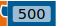
\includegraphics[width=0.05\textwidth]{./pics/zahlargument1.png} Zahlenwerte: 
		
		Sowohl ganze Zahlen als auch Dezimalzahlen (mit Punkt als Komma),
		\item 
\includegraphics[width=0.1\textwidth]{./pics/textargument.png} Zeichenketten: 
		
		Aneinanderreihung von Zeichen.
	\end{itemize}
\end{zsfg}

\vfill

\section{Entscheidungen mit mehreren Kriterien treffen}
\label{sec:wahrheitswerte}

Bisher waren die zu treffenden Entscheidungen immer nur von einem Kriterium abhängig. Das sind jedoch Ausnahmen. Nun geht es darum, wie man mehrere Kriterien miteinander kombinieren kann.

\begin{ziel}
	\textbf{Frage:} Wie lassen sich Entscheidungen mit mehreren Kriterien programmieren?
\end{ziel}

\begin{projekt}[Carport-Lampe]\label{proj:carportlampe}
	Baue und programmiere eine Carport-Lampe, die für einige Zeit leuchtet, wenn sie eine Bewegung registriert \tcbox[size=fbox,box align = base,colback=nepoLogik, colframe=gray,nobeforeafter]{\color{white}\bfseries\texttt{und}} es draußen gerade dunkel ist. In allen anderen Fällen bleibt die Lampe dunkel. Experimentiere mit den Drehreglern, um die Empfindlichkeit und Dauer des Signals richtig einzustellen.
\end{projekt}

\emph{Information zu Bewegungsmeldern:} Bewegungsmelder verfügen über drei Pins, deren Beschriftung man lesen kann, wenn man die Kunststofflinse vorsichtig abzieht (\emph{Vorsicht: Nach Abziehen der Linse nicht den Sensor berühren!}). \texttt{Vcc} und \texttt{GND} dienen der Stromversorgung der elektronischen Komponenten und müssen mit \texttt{5\,V} und \texttt{GND} am Arduino verbunden werden. 

Der mittlere \texttt{OUT}-Pin ist der Signal-Pin: Wenn eine Bewegung registriert wurde, wird der Wert \texttt{wahr} zurückgegeben, ansonsten \texttt{falsch}. Zum Einlesen des Signals wird dieser Pin mit einem Digitalpin des Arduino verbunden.

Hinten befinden sich zwei Drehregler (\enquote{Potentiometer}), mit denen sich die Dauer des Bewegungssignals (links) und die Empfindlichkeit (rechts) einstellen lassen. Zusätzlich befindet sich auf der rechten Seite ein sogenannter Jumper, mit dem auf einfache Weise eine Steckverbindung zwischen benachbarten Pins hergestellt werden kann. Wenn sich der Jumper ganz außen befindet, dann bleibt das Bewegungssignal nach dem Erkennen einer Bewegung eine Weile aktiv und wird dann auf jeden Fall deaktiviert. Eine neue Bewegung kann erst nach einer gewissen Zeit wieder registriert werden. Wenn der Jumper hingegen leicht nach innen versetzt ist, bleibt das Bewegungssignal so lange erhalten, wie eine Bewegung erkannt wird (siehe \href{https://funduino.de/nr-8-bewegungsmelder}{Funduino}).

\begin{minipage}{0.3\textwidth}
	\begin{figure}[H]
		\centering
		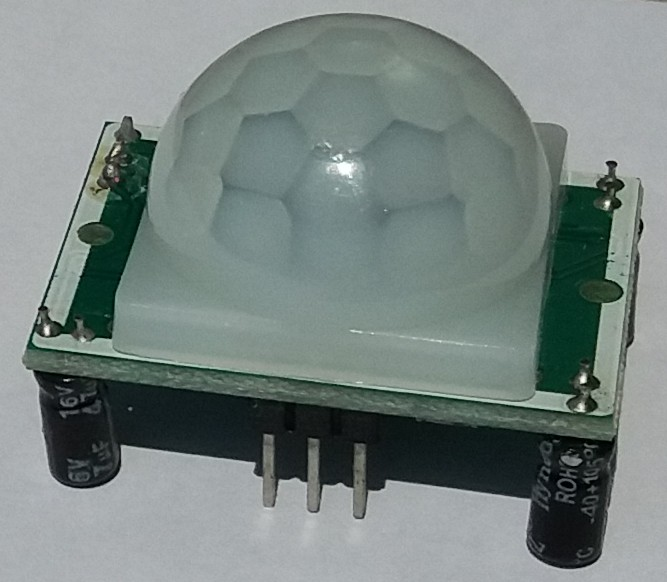
\includegraphics[width=0.67\textwidth]{pics/bewegungsmelder.jpg}
		\caption{Bewegungsmelder mit Linse.}
		\label{abb:bewegungsmelder}
	\end{figure}
\end{minipage}
\hfill
\begin{minipage}{0.3\textwidth}
	\begin{figure}[H]
		\centering
		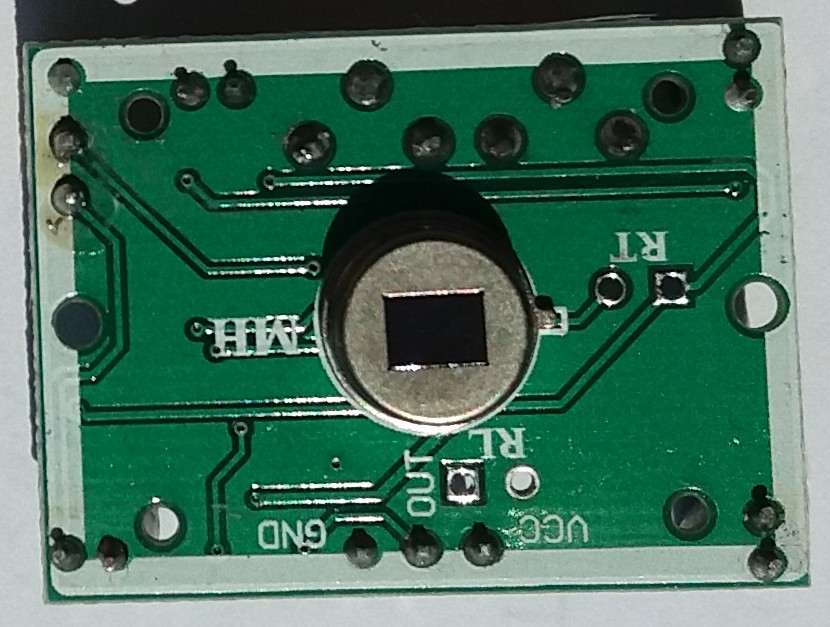
\includegraphics[width=0.83\textwidth]{pics/bewegungsmelder-ohne-linse.jpg}
		\caption{Pinbelegung.}
		\label{abb:bewegungsmelder-ohne-linse}
	\end{figure}
\end{minipage}
\hfill
\begin{minipage}{0.3\textwidth}
	\begin{figure}[H]
		\centering
		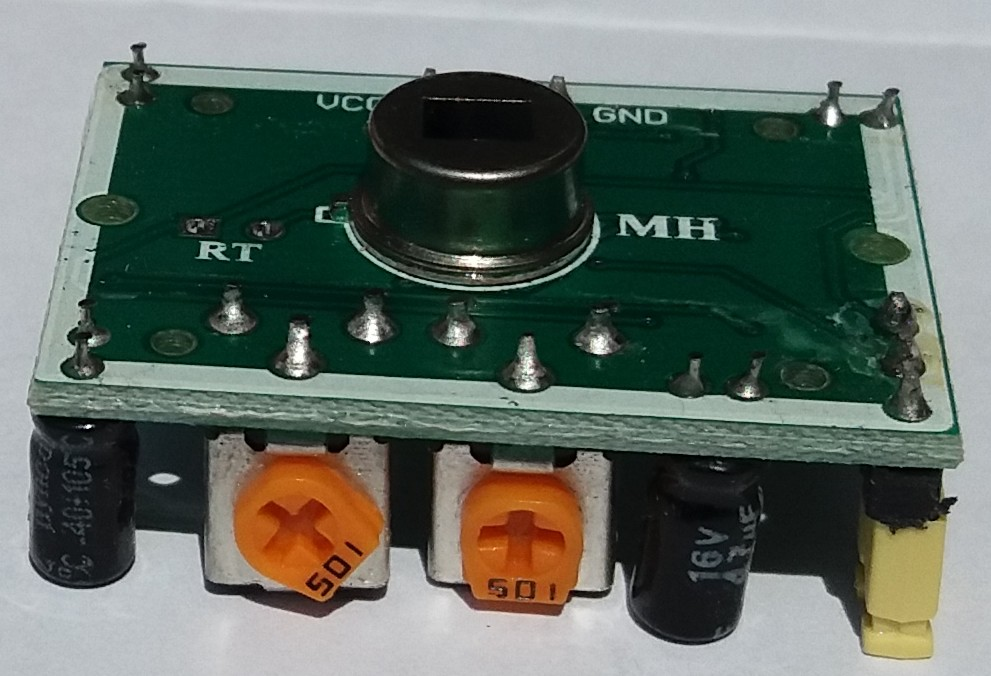
\includegraphics[width=0.83\textwidth]{pics/bewegungsmelder-hinten.jpg}
		\caption{Drehregler für Signaldauer (links) und Empfindlichkeit (rechts).}
		\label{abb:bewegungsmelder-hinten}
	\end{figure}
\end{minipage}

\vfill

\newpage
\begin{aufgabe} \emph{Wahrheitswerttabellen}
	\marginpar{%
		~\\
		~\\
		\footnotesize%
		\textattachfile[description={Arbeitsblatt zu Kap. \thechapter, Wahrheitswerttabellen}]{./Auftraege/kap3-ab-wahrheitswerttabellen.pdf}{
			\footnotesize%
			\drucker Arbeitsblatt%
		}
		\\öffnen%
	}
	\begin{enumerate}[label=\alph*), itemsep=0ex, parsep=0ex]
		\item Experimentiere mit der Carport-Lampe, um die folgende Wahrheitswert-Tabelle für die Operation UND auszufüllen.
		
			\medskip
			\begin{minipage}{0.4\textwidth}
				A: Bewegung registriert.
				
				B: Es ist dunkel.
			\end{minipage}
			\hfill
			\begin{minipage}{0.4\textwidth}
				\centering
				\begin{tabular}{c | c | c}
					\textbf{A} & \textbf{B} & \textbf{A UND B} \\ \hline
					wahr & wahr &  \\
					&  &  \\
					&  &  \\
					&  &  \\  
				\end{tabular}
			\end{minipage}
			\hfill
		
		\medskip
		\item Ändere das UND zu einem ODER und experimentiere wieder mit der Carport-Lampe, um die folgende Wahrheitswert-Tabelle für die Operation ODER auszufüllen.
		
			\medskip
			\begin{minipage}{0.4\textwidth}
				A: Bewegung registriert.
				
				B: Es ist dunkel.
			\end{minipage}
			\hfill
			\begin{minipage}{0.4\textwidth}
				\centering
				\begin{tabular}{c | c | c}
					\textbf{A} & \textbf{B} & \textbf{A ODER B} \\ \hline
					wahr & wahr &  \\
					&  &  \\
					&  &  \\
					&  &  \\  
				\end{tabular}
			\end{minipage}
			\hfill
		
		\medskip
		\item Ergänze die Wahrheitswerttabelle für die logische Operation NICHT.
			
			\medskip
			\begin{minipage}{0.4\textwidth}
				
			\end{minipage}
			\hfill
			\begin{minipage}{0.4\textwidth}
				\centering
				\begin{tabular}{c | c}
					\textbf{A}  & \textbf{NICHT A} \\ \hline
					wahr &  \\
					falsch &  \\  
				\end{tabular}
			\end{minipage}
			\hfill
	\end{enumerate}
\end{aufgabe}


\begin{zsfg}{Logische Operationen und Wahrheitswerttabellen}
	
	Logische Operationen dienen zum Verknüpfen von Wahrheitswerten - ganz so wie Rechenoperationen zum Verknüpfen von Zahlen dienen. Wir betrachten die logischen Operationen UND (AND), ODER (OR) sowie NICHT (NOT). Das Ergebnis dieser Operationen lässt sich anhand von Wahrheitswerttabellen übersichtlich festhalten. Darin wird festgehalten, ob zwei Aussagen bzw. Bedingungen A und B wahr (w) oder falsch (f) sind. In der rechten Spalte steht dann, ob die logische Operation wahr (w) oder falsch (f) ergibt.
	
	\medskip
	\begin{minipage}{0.3\textwidth}
		\centering
		\begin{tabular}{c | c | c}
			\textbf{A} & \textbf{B} & \textbf{A UND B} \\ \hline
			w & w & w \\
			w & f & f \\
			f & w & f \\
			f & f & f \\  
		\end{tabular}
	\end{minipage}
	\hfill
	\begin{minipage}{0.3\textwidth}
		\centering
		\begin{tabular}{c | c | c}
			\textbf{A} & \textbf{B} & \textbf{A ODER B} \\ \hline
			w & w & w \\
			w & f & w \\
			f & w & w \\
			f & f & f \\  
		\end{tabular}
	\end{minipage}
	\hfill
	\begin{minipage}[t]{0.3\textwidth}
		\centering
		\begin{tabular}{c | c}
			\textbf{A}  & \textbf{NICHT A} \\ \hline
			w & f \\
			f & w \\  
		\end{tabular}
	\end{minipage}
	
	\medskip
	Achtung: Die ODER-Operation ergibt auch dann \enquote{wahr}, wenn beide Aussagen wahr sind. Das aus dem Alltag bekannte \enquote{ENTWEDER-ODER} (XOR) ist eine weitere logische Operation, die \enquote{falsch} ergibt, wenn beide Aussagen wahr sind. Diese Operation ist aber nicht in Nepo enthalten.
\end{zsfg}

\begin{aufgabe} \emph{Verschachtelte Entscheidungen?!}
	
	Leo und Lara möchten ihre Carport-Lampe so umprogrammieren, dass sie nachts immer leuchtet und tagsüber nicht. Zusätzlich soll ein Alarm ertönen, wenn es Nacht ist und eine Bewegung registriert wird.
	
	Unten sind ihre Programme abgebildet. Entscheide jeweils (begründet!), ob das Programm für das geforderte Verhalten geeignet ist. Mache gegebenenfalls Verbesserungsvorschläge.
	
	\bigskip
	\begin{figure}[H]
		\begin{adjustwidth*}{-1.5cm}{-1.5cm}
			\centering
			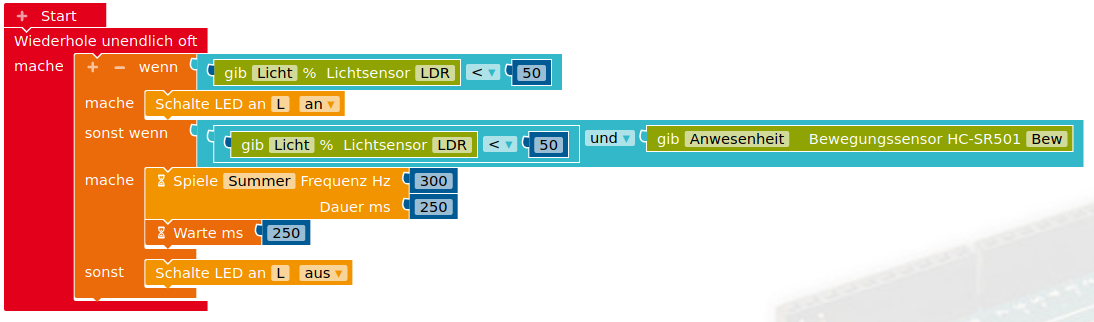
\includegraphics[width=1.2\textwidth]{./pics/wenn-sonstWenn-sonst-Bsp.png}
			\caption{Leos Programm.}
			\label{abb:sonstWenn1}
		\end{adjustwidth*}
	\end{figure}
	\begin{figure}[H]
		\begin{adjustwidth*}{-1.5cm}{-1.5cm}
			\centering
			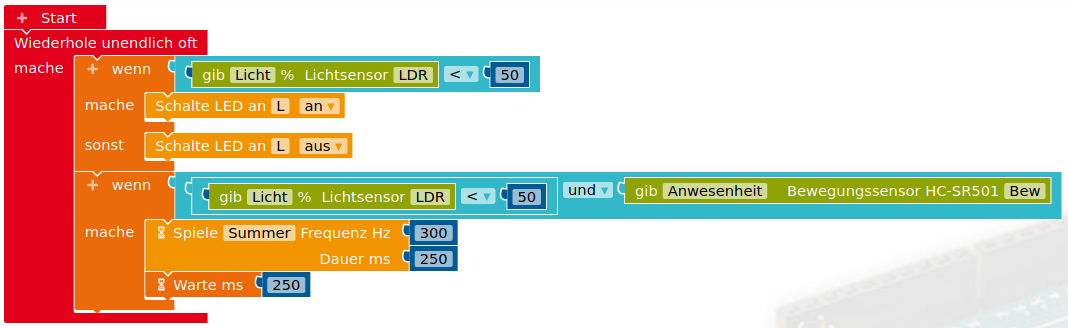
\includegraphics[width=1.2\textwidth]{./pics/wenn-sonstWenn-sonst-Bsp2.png}
			\caption{Laras Programm.}
		\end{adjustwidth*}
	\end{figure}
\end{aufgabe}

\newpage
\section{Programme mit Variablen und Schleifen effizient steuern}
\label{sec:variablenUndSchleifen}

\begin{aufgabe}
	Jana und Jonas haben jeweils LEDs an den Arduino angeschlossen und steuern diese mit den unten abgebildeten Programmen. Vergleiche die beiden Programme im Hinblick auf ihre Wirkung und die Art der Programmierung. Welches gefällt dir besser?
	
	Zusatzüberlegung: Wie viel muss man ändern, wenn man die Leuchtdauer ändern will?
\end{aufgabe}
\marginpar{%
	\textattachfile[description={Folie zu Kap. \thechapter, Variableneinsatz}]{./Auftraege/kap3-auftrag-variablen.pdf}{%
		\footnotesize\folie Folie %
	}%
	\footnotesize%
	\\öffnen%
}

\begin{figure}[H]
	\begin{minipage}{0.48\textwidth}
		\centering
		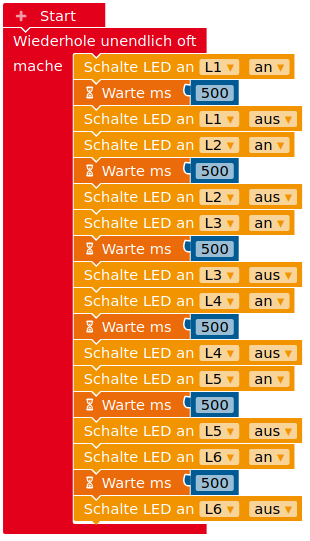
\includegraphics[width=0.8\textwidth]{./pics/lauflicht-ohne-variable.png}
		\caption{Janas Programm zum Steuern der LEDs.}
	\end{minipage}
	\hfill
	\begin{minipage}{0.48\textwidth}
		\centering
		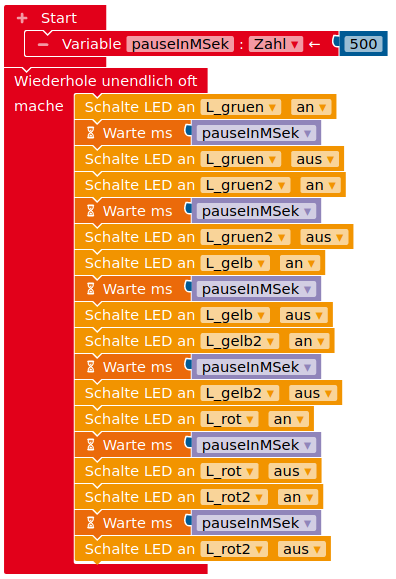
\includegraphics[width=\textwidth]{./pics/lauflicht-mit-variable.png}
		\caption{Jonas Programm zum Steuern der LEDs.}
	\end{minipage}
\end{figure}

\vspace{-0.5\baselineskip}
\begin{zsfg}{Variablen}
	\begin{wrapfigure}{r}{0.3\textwidth}
		\begin{tikzpicture}[scale=0.5]
		\draw (-0.2,0) -- (5.2,0);
		\draw (-0.2,1) -- (5.2,1);
		\draw [fill=white] (0,0) rectangle (0.8,1);
		\draw [fill=white] (0.8,0) rectangle (4.2,1);
		\draw [fill=white] (4.2,0) rectangle (5,1);
		\node (pause) at (2.5,0.5) {\sffamily\scriptsize pauseInMSek};
		\draw (5.8,0.2) -- (5.8,-4);
		\draw (8.2,0.2) -- (8.2,-4);
		\draw [fill=gray!40] (5.8,-1) rectangle (8.2,-3.5);
		\node (wert) at (7,-2.25) {\sffamily\scriptsize 500};
		\draw [gray!30!black, thick,->] (pause) to [out=270,in=140] (wert);
		\node at (7,-3) {\sffamily\scriptsize Speicher};
		\end{tikzpicture}
	\end{wrapfigure}
	Eine Variable kann man sich als Koffer vorstellen, der einen Namen bekommt und in dem man einen festgelegten Datentyp speichert. Jedes Mal, wenn der Name des Koffers aufgerufen wird, wird der abgespeicherte Wert hervorgeholt und an die Stelle des Namens gesetzt. Intern wird der Variablenname als Verweis auf einen bestimmten Speicherplatz genutzt, in dem der Wert der Variable abgelegt ist.
	
	Für den Namen hat sich der \href{https://de.wikipedia.org/wiki/Binnenmajuskel#Programmiersprachen}{lowerCamelCase} etabliert: Der erste Buchstabe ist klein; wenn weitere Wörter folgen, fangen diese mit einem großen Buchstaben an. Leerzeichen sind nicht erlaubt.
\end{zsfg}

\subsection{Zufällige Ereignisse und Wiederholungen programmieren}


\begin{wrapfigure}{r}{0.4\textwidth}
	\quad \nepoexpert
	\begin{center}
		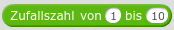
\includegraphics[width=0.4\textwidth]{./pics/zufallszahl.png}
	\end{center}
\end{wrapfigure}
Viele Dinge werden interessanter, wenn sie sich nicht immer auf die genau gleiche Art wiederholen. Für diese Fälle kann man im Programm den blauen Block für Zufallszahlen verwenden (Expertenblöcke aktivieren!), der jedes Mal eine neue Zufallszahl erzeugt, wenn er aufgerufen wird. Ein einfaches Beispiel ist die \enquote{Bombe}, die man bei dem Spiel \enquote{Tick Tack Bumm} startet und die man so lange herum geben muss, bis sie explodiert. Dabei ist die Dauer des Tickens ein zufälliger Wert zwischen ca. 5\,s und 20\,s.
\marginpar{%
	\footnotesize%
	\video \\
	\href{https://el-voss.de/downloads/ticktack.html}{Bomben-Beispielvideo}
}

\bigskip
\begin{minipage}{0.73\textwidth}
	\begin{projekt}[Bombe bauen]\label{proj:bombe}
		Baue und programmiere eine \enquote{Bombe}, die für eine zufällige Dauer zwischen 5\,s und 20\,s tickt und dann explodiert. Die Bombe wird über einen Taster aktiviert.
		
		Zusatz: Welchen Unterschied macht es, wenn man die ausgewürfelte Zufallszahl in einer Variable speichert?
	\end{projekt}
\end{minipage}
\hfill
\begin{minipage}{0.25\textwidth}
	\centering
	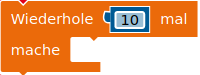
\includegraphics[width=0.8\textwidth]{./pics/wdh10mal.png}
\end{minipage}

\bigskip

\begin{aufgabe} \emph{Exkurs: Zufallszahlen von Mikrocontrollern/Mikroprozessoren}
	
	\begin{wrapfigure}{r}{0.7\textwidth}
		\centering
		\vspace{-0.5\baselineskip}
		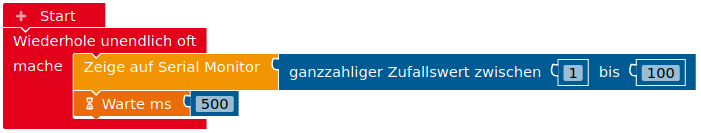
\includegraphics[width=0.7\textwidth]{./pics/zufallszahlengenerator.png}
	\end{wrapfigure}
	Übertrage das rechts abgebildete Programm auf den Arduino und betrachte die so erzeugten Zufallszahlen. Drücke dann auf den Reset-Taster am Arduino und betrachte die nun erzeugten Zufallszahlen. Wiederhole den Vorgang einige Male und beschreibe Auffälligkeiten.
\end{aufgabe}

%Reaktionszeitmesser mit Zufallselement; Aufgabe: Struktogramm

\bigskip
\begin{projekt}[Reaktionszeitmesser]\label{proj:reaktionszeitmesser}
	Baue und programmiere einen Reaktionszeitmesser.
	
	\begin{wrapfigure}{r}{0.3\textwidth}
		\centering
		
\includegraphics[width=0.28\textwidth]{./pics/stoppuhr2.png}
		\includegraphics[width=0.28\textwidth]{./pics/stoppuhr.png}
	\end{wrapfigure}
	Der Reaktionszeitmesser soll zunächst warten, bis ein Taster gedrückt wurde, der besagt, dass es losgehen kann. Dann wird eine LED angeschaltet (Vorwiderstand!) und nach einer zufälligen Zeit wieder ausgeschaltet. Nun beginnt die Zeitmessung. Die Stoppuhr läuft solange, bis der Taster gedrückt wurde. Die gemessene Zeit wird dann über den seriellen Monitor ausgegeben und es wird erneut gewartet, bis der Anwender bestätigt, dass es losgehen kann.
	
	Miss mindestens zehn Mal deine Reaktionszeit und bestimme den Mittelwert. Bist du besser als dein Partner?
	
	{\scriptsize Idee: Frick, Fritsch und Trick (2015): \emph{Einführung in Mikrocontroller - Der Arduino als Steuerzentrale}, Bad Saulgau}
\end{projekt}

\subsection{Wiederholungen mit Bedingungen steuern}
\label{sec:while-schleife}

In vielen Fällen geht es bei Schleifen nicht um eine genau oder zufällig bestimmte Anzahl von Wiederholungen, sondern darum, einen Vorgang zu wiederholen, bis eine Bedingung wahr ergibt, bzw. solange, wie eine Bedingung wahr ergibt. Die Bedingung, die wahr oder falsch ergibt, kann auch Sensorwerte beinhalten. Dies wird auch im folgenden Spiel genutzt.

\bigskip
\begin{projekt}[Konfigurierbares Reaktionsspiel]\label{proj:reaktionsspiel}
	Baue und programmiere ein konfigurierbares Reaktionsspiel!
	
	\begin{wrapfigure}{r}{0.4\textwidth}
		\begin{tikzpicture}
		\draw (0,6) rectangle (6,6.5) node at (0.5,6.25) [right] {\sffamily\footnotesize Serial Monitor};
		\draw [fill=gray!20] (0,0) rectangle (6,6);
		\node at (0.25,5.5) [right] {\sffamily\scriptsize Willkommen beim Reaktionsspiel!};
		\node at (0.25,5) [right] {\sffamily\scriptsize Stelle zuerst die max. Reaktionszeit ein.};
		\node at (0.25,4.5) [right] {\sffamily\scriptsize Max. Reaktionszeit in Millisekunden:};
		\node at (0.25,4) [right] {\sffamily\scriptsize 500};
		\node at (0.25,3.5) [right] {\sffamily\scriptsize Max. Reaktionszeit in Millisekunden:};
		\node at (0.25,3) [right] {\sffamily\scriptsize 490};
		\node at (0.25,2.5) [right] {\sffamily\scriptsize Spiel startet...};
		\node at (0.25,2) [right] {\sffamily\scriptsize Drücke Taster:};
		\node at (0.25,1.5) [right] {\sffamily\scriptsize 2};
		\node at (0.25,1) [right] {\sffamily\scriptsize Taster 2 gedrückt};
		\node at (0.25,0.5) [right] {\sffamily\scriptsize Sehr gut!};
		\end{tikzpicture}
	\end{wrapfigure}
	
	\medskip
	Dazu werden drei Taster (mit Widerstand!) am Arduino angeschlossen. Nach einer zufälligen Zeit wird auf dem seriellen Monitor angezeigt, welcher (zufällig ausgewürfelte) Taster gedrückt werden soll. Geschieht dies innerhalb einer vorgegebenen maximalen Reaktionszeit, hat man gewonnen, andernfalls verloren.
	
	Am Anfang des Spiels soll diese maximale Reaktionszeit konfiguriert werden können. Das heißt, man kann die max. Reaktionszeit mit dem linken Taster verringern und mit dem rechten Taster vergrößern. Erst wenn der mittlere Taster gedrückt wird, startet das Spiel.
	
	\medskip
	Für einen besseren Zugang zu diesem komplexen Spiel kannst du folgende Vorlage öffnen, mittels \enquote{Speichern unter} als \texttt{Reaktionsspiel.xml} auf dem Computer speichern und die Datei im Open Roberta Lab importieren:
	\textattachfile[mimetype=text/plain, description={Vorlage zur Programmierung eines frei konfigurierbaren Reaktionsspiels}]{./lsg/NEPO-Reaktionsspiel-Start.xml}{
		reaktionsspiel-vorlage.xml%
	}.
\end{projekt}

\emph{Mögliche Erweiterungen:}
\begin{itemize}[itemsep=0ex, parsep=0ex]
	\item zusätzliche Ausgabe der Reaktionszeit,
	\item Ober- und Untergrenze für die einstellbare maximale Reaktionszeit, damit das Spiel nicht unmöglich, aber auch nicht zu langweilig wird,
	\item nach Spielstart folgen mehrere Spiele hintereinander und es wird mitgezählt, wie oft gewonnen wird,
	\item je nach Reaktionszeit bekommt man mehr oder weniger Punkte,
	\item \dots
\end{itemize}

\newpage
\subsection{Zählschleifen programmieren}
\label{sec:for-schleife}

Lauflichter findet man inzwischen überall in unserer Welt: An den Rändern von Landebahnen an Flughäfen, an Spieleautomaten, aufdringlichen Werbeschildern, als Blinker von modernen Autos und vieles mehr. Wenn man diese programmieren will, eignen sich dazu am besten Zählschleifen.

\medskip
\begin{aufgabe} \emph{Zählschleifen verstehen}
	
	\begin{wrapfigure}{r}{0.7\textwidth}
		\centering
		\vspace{-0.5\baselineskip}
		\includegraphics[width=0.68\textwidth]{./pics/for-schleife-bsp.png}
	\end{wrapfigure}
	Das rechts abgebildete Programm enthält zwei selbst definierte Blöcke, mit denen sich eine LED an einem beliebigen Pin zwischen 2 und 13 anstellen bzw. ausschalten lässt. In der Endlosschleife wird dann eine Zählschleife genutzt.
	
	\medskip
	Stelle eine Vermutung an, was die Zählschleife bewirkt.
	
	\medskip
	Überprüfe deine Vermutung mit Hilfe einer \emph{Trace-Tabelle} (siehe unten).
\end{aufgabe}

\begin{zsfg}{Trace-Tabellen}
	\begin{minipage}{0.78\textwidth}
		Trace-Tabellen stellen den Wert von Variablen beim Durchlaufen des Programms dar. Auf diese Art und Weise kann man sich zum Beispiel genau veranschaulichen, wann Schleifen abgebrochen werden.
	\end{minipage}
	\hfill
	\begin{minipage}{0.2\textwidth}
		\centering
		\scriptsize
		\begin{tabular}{l | c}
			\textbf{Zeile} & \textbf{i} \\ \hline
			\dots & \dots \\ \hline
			5 & 2 \\ \hline
			6 & 2 \\ \hline
			5 & 3 \\ \hline
			6 & 3 \\ \hline
		\end{tabular}
	\end{minipage}	
\end{zsfg}

\bigskip
\marginpar{%
	\footnotesize%
	\video \\
	\href{https://www.youtube.com/watch?v=s317_5aFL6E}{Blinker-Beispielvideo}
}
\begin{projekt}[Auto-Blinker]\label{proj:blinker}
	Programmiere ein Lauflicht so, wie es auch als Blinker in modernen Autos genutzt wird. Nutze zunächst nur 5 LEDs (mit Vorwiderstand!).
	
	\medskip
	\emph{Hinweis:} Du kannst das folgende Programm als Vorlage nutzen, damit du auch über die selbst definierten Blöcke zum Anstellen bzw. Ausstellen einer LED an einem beliebigen Pin zwischen 2 und 13 verfügst. Öffne das Programm, speichere es als \texttt{blinker.xml} und importiere es in Open Roberta Lab:
	\textattachfile[mimetype=text/plain, description={Vorlage zur Programmierung eines Lauflichtes}]{./lsg/NEPO-lauflicht-start.xml}{
		blinker-vorlage.xml%
	}.
\end{projekt}

\begin{aufgabe} \emph{La - o - La}
	
	Programmiere ein Lauflicht, das hin- und zurückläuft.
\end{aufgabe}

\vfill

\begin{aufgabe} \emph{Steuerung von Schleifen}
	
	Unten siehst du zwei Programme, für die jeweils fünf LEDs mit Vorwiderstand an Pin 2 bis 6 angeschlossen wurden. Baue das nach, importiere die Programme in Open Roberta Lab und übertrage sie auf den Arduino.
	
	Beschreibe die Wirkung von \texttt{Die Schleife abbrechen} und \texttt{mit der nächsten Iteration der Schleife fortfahren}.
	
	\bigskip
	\begin{minipage}{0.48\textwidth}
		\centering
		\includegraphics[width=\linewidth]{./pics/break-bsp.png}
		\bigskip
		\textattachfile[mimetype=text/plain, description={Vorlage zur Untersuchung eines Schleifenabbruchs}]{./lsg/NEPO-break-Bsp.xml}{
			schleife-abbrechen.xml%
		}
	\end{minipage}
	\hfill
	\begin{minipage}{0.48\textwidth}
		\centering
		\includegraphics[width=\linewidth]{./pics/continue-bsp.png}
		\bigskip
		\textattachfile[mimetype=text/plain, description={Vorlage zur Untersuchung eines Schleifensprungs}]{./lsg/NEPO-continue-Bsp.xml}{
			schleife-fortfahren.xml%
		}
	\end{minipage}
\end{aufgabe}

\bigskip
In Nepo wie in anderen Programmiersprachen gibt es verschiedene Arten von Schleifen. Bisher wurde in Nepo die einfache Zählschleife \texttt{wiederhole x mal}, die bedingungsgesteuerte Wiederholschleife \texttt{wiederhole bis / solange} und die Zählschleife mit Zählervariable genutzt. Tatsächlich lässt sich das gleiche Verhalten aber mit allen drei Schleifenvarianten erreichen.

\begin{aufgabe} \emph{Vergleich von Schleifen}
	
	Betrachte noch einmal das Programm \texttt{schleife-abbrechen.xml} (siehe oben). Implementiere das gleiche Verhalten mit \dots
	\begin{enumerate}[label=\alph*), itemsep=0ex, parsep=0ex]
		\item \dots einer \texttt{wiederhole x mal} Schleife,
		\item \dots einer \texttt{wiederhole bis} Schleife,
		\item \dots einer \texttt{wiederhole solange} Schleife.
	\end{enumerate}

	Erkläre, welche Schleifenvariante sich als \enquote{Grundschleife} eignet, die die anderen Varianten \emph{immer} ersetzen kann.
\end{aufgabe}

\newpage
\begin{zsfg}{Sichtbarkeit: Lokale und globale Variablen}
	Ein Unterschied zwischen den Schleifenimplementierungen bleibt bestehen: Die Zählvariable \texttt{i} wird bei einer Zählschleife als \emph{lokale Variable} angelegt, das heißt, man kann die Zählvariable nur \emph{innerhalb der Schleife} nutzen. Dafür benötigt sie auch nur innerhalb der Schleife Speicherplatz.
	
	Im Gegensatz dazu sind die unter \texttt{Start} angelegten Variablen überall im Programm bzw. global verfügbar und heißen deshalb \emph{globale Variablen}. Für diese Variablen muss während der ganzen Zeit Speicherplatz bereitgehalten werden, auch wenn sie vielleicht nur an einer Stelle wirklich benötigt werden.
\end{zsfg}

\begin{zsfg}{Schleifen}
	
	Bei der Programmierung werden häufig Schleifen genutzt, die die Anweisungen in ihrem Rumpf (oder Körper) solange wiederholen, bis eine gewisse Abbruchbedingung eintritt.
	
	\begin{itemize}[itemsep=0ex, parsep=0ex]
		\item \texttt{wiederhole x mal}: Einfache \emph{Zählschleife}, die die Anweisungen im Rumpf für eine festgelegte Anzahl wiederholt.
		\item \texttt{wiederhole, bis}: Bedingungsgesteuerte Schleife, die die Anweisungen im Rumpf wiederholt, \emph{bis} die Bedingung wahr ergibt.
		\item \texttt{wiederhole, solange}: Bedingungsgesteuerte Schleife, die die Anweisungen im Rumpf wiederholt, \emph{solange} die Bedingung wahr ergibt.
		\item \texttt{zähle i von \dots ~solange Zähler \dots ~mit Schrittweite \dots}: Zählergesteuerte Schleife, die die Anweisungen im Rumpf wiederholt, solange der Zähler kleiner als eine vorgegebene Zahl ist und die Zählervariable nach jedem Durchlauf um eine angegebene Zahl erhöht.
	\end{itemize}
		
	Die Überprüfung, ob die Bedingung wahr ist, erfolgt hier \emph{vor} der Ausführung der Anweisungen im Rumpf. Daher nennt man die Schleifen auch \emph{kopfgesteuert}.
\end{zsfg}


\newpage
\section{Programme mit Struktogrammen dokumentieren}
\label{sec:struktogramme}

Wenn wir uns über Programme austauschen, dann haben wir nicht immer den Computer zur Hand. In solchen Momenten wäre es viel zu aufwendig, die bunten Blöcke von Nepo zu malen. Außerdem könnte es sein, dass jemand anderes das Programm nicht mit Blöcken, sondern mit Text in der Programmiersprache C++ aufschreiben will, also so wie der ~\nepoquellcode Quellcode aussieht.

\begin{ziel}
	\textbf{Frage:} Wie kann man Programme übersichtlich zu Papier bringen?
\end{ziel}

Man nutzt zur Darstellung des Ablaufs eines Computerprogramms sogenannte \textbf{Struktogramme} (vgl. Tab. \ref{tab:struktogramm}), die in den 1970er Jahren von Isaac Nassi und Ben Shneidermann entwickelt wurden. Struktogramme sollen ein Computerprogramm möglichst einfach und ohne programmiersprachenspezifische Befehlssyntax abbilden. Auf diese Art und Weise lassen sich Programme auch einfach planen, bevor man sich damit beschäftigt, wie die Schritte im Einzelnen zu codieren sind.

\begin{aufgabe}
	Stelle die unten abgebildeten Programme jeweils mithilfe eines Struktogramms dar.
\end{aufgabe}

\begin{figure}[H]
	\begin{adjustwidth}{-1.5cm}{1.5cm}
		\centering
		\includegraphics[width=1.2\textwidth]{./pics/wenn-sonstWenn-sonst-Bsp2.png}
		\caption{Programm A.}
	\end{adjustwidth}
\end{figure}
%\vspace{-\baselineskip}
\begin{figure}[H]
	\centering
	\includegraphics[width=0.7\textwidth]{./pics/break-bsp-schmal.png}
	\caption{Programm B.}
\end{figure}

\newpage

\begin{zsfg}{Darstellung von Programmen in Struktogrammen}
	
	\begin{table}[H]
		\centering
		\begin{minipage}[b]{\textwidth}
			\begin{tabu} to \textwidth {X[L,3]X[L,2]}
				\toprule
				\vspace{-4\baselineskip}
				\textbf{Lineare Struktur}
				
				Jede Anweisung wird in einen rechteckigen Block geschrieben.
				
				&
				\begin{tikzpicture}
				\draw (0,0) rectangle (5,1);
				\node at (2.5,0.5) {\footnotesize Anweisung 2};
				\draw (0,1) rectangle (5,2);
				\node at (2.5,1.5) {\footnotesize Anweisung 1};
				\end{tikzpicture}
				\\
				\midrule%\hline
				%\rowcolor{CadetBlue!80!green}
				\textbf{Wiederholung / Schleifen} & \\
				\midrule%\hline
				%         \vspace{-4.2\baselineskip}
				\vspace{0mm}
				\textbf{Zählergesteuerte Schleife}
				
				Die Anzahl der Schleifendurchläufe wird durch eine Zählvariable festgelegt. Im Schleifenkopf werden der Startwert der Zählvariablen, der Endwert der Zählvariablen und die Veränderung der Zählvariablen, z.\,B. Schrittweite 1, angegeben.
				&
				\smallbreak
				\vspace{-0.7\baselineskip}
				\begin{tikzpicture}
				\fill [CadetBlue!70!green] (0,0) rectangle (5,2.2);
				\draw (0,0) -- (0,2) -- (5,2) -- (5,1) -- (0.2,1) -- (0.2,0) -- (0,0);
				\draw (0.2,0) -- (5,0) -- (5,1);
				\node at (2.5,0.5) {\footnotesize Anweisung 1};
				\node at (2.5,1.5) {\parbox{4cm}{\scriptsize zähle Variable von Startwert bis Endwert, Schrittweite}};
				\end{tikzpicture}
				\\
				\midrule
				\vspace{-4\baselineskip}
				\textbf{Kopfgesteuerte Schleife}
				
				Wiederholungsschleife mit vorausgehender Prüfung der Bedingung. Der Schleifenkörper wird so lange wiederholt, \emph{wie} oder \emph{bis} die Bedingung wahr ist (bei uns nur der letzte Fall verfügbar).
				&
				\begin{tikzpicture}
				\draw (0,0) -- (0,2) -- (5,2) -- (5,1) -- (0.2,1) -- (0.2,0) -- (0,0);
				\draw (0.2,0) -- (5,0) -- (5,1);
				\node at (2.5,0.5) {\footnotesize Anweisung 1};
				\node at (2.5,1.5) {\footnotesize solange, wie/bis Bedingung wahr};
				\end{tikzpicture}
				\\
				\midrule
				\vspace{-4\baselineskip}
				\textbf{Fußgesteuerte Schleife}
				
				Wiederholungsschleife mit nachfolgender Prüfung der Bedingung. Der Schleifenkörper wird so lange wiederholt, \emph{wie} oder \emph{bis} die Bedingung wahr ist (in mBlock nicht verfügbar).\smallskip
				&
				\begin{tikzpicture}
				\draw (0,0) -- (0,2) -- (0.2,2) -- (0.2,1) -- (5,1) -- (5,0) -- (0,0);
				\draw (0.2,2) -- (5,2) -- (5,1);
				\node at (2.5,1.5) {\footnotesize Anweisung 1};
				\node at (2.5,0.5) {\footnotesize solange, wie/bis Bedingung wahr};
				\end{tikzpicture}
				\\
				\midrule%\hline
				%\rowcolor{CadetBlue!80!green}
				\textbf{Verzweigung} & \\
				\midrule%\hline
				\vspace{0mm}
				\textbf{Einfache Verzweigung}
				
				Die Anweisung 1 (und ggf. weitere) wird nur ausgeführt, falls die Bedingung wahr ist. Andernfalls wird nichts gemacht.
				&
				\smallbreak
				\vspace{-0.7\baselineskip}
				\begin{tikzpicture}[scale=0.7]
				\fill [CadetBlue!70!green] (0,0) rectangle (8,2.7);
				\draw (0,0) rectangle (8,2.5);
				\draw (0,1) -- (8,1);
				\draw (4,0) -- (4,1) -- (8,2.5);
				\draw (4,1) -- (0,2.5);
				\node at (2,0.5) {\footnotesize Anweisung 1};
				\node at (1,1.5) {\footnotesize ja};
				\node at (7,1.5) {\footnotesize nein};
				\node at (4,2) {\footnotesize Bedingung};
				\end{tikzpicture}
				\\
				\midrule
				\vspace{-3.5\baselineskip}
				\textbf{Alternative Verzweigung}
				
				Falls die Bedingung wahr ist, wird Anweisung 1 (und ggf. weitere) ausgeführt, sonst wird Anweisung 2 (und ggf. weitere) ausgeführt.
				&
				\begin{tikzpicture}[scale=0.7]
				\draw (0,0) rectangle (8,2.5);
				\draw (0,1) -- (8,1);
				\draw (4,0) -- (4,1) -- (8,2.5);
				\draw (4,1) -- (0,2.5);
				\node at (2,0.5) {\footnotesize Anweisung 1};
				\node at (6,0.5) {\footnotesize Anweisung 2};
				\node at (1,1.5) {\footnotesize ja};
				\node at (7,1.5) {\footnotesize nein};
				\node at (4,2) {\footnotesize Bedingung};
				\end{tikzpicture}
				\\
				\midrule
				\vspace{-5.5\baselineskip}
				\textbf{Verschachtelte Verzweigung}
				
				Falls Bedingung 1 wahr ist, folgt eine weitere Bedingung 2.
				&
				\begin{tikzpicture}[scale=0.7]
				\draw (0,-1.5) rectangle (8,2.5);
				\draw (0,1) -- (8,1);
				\draw (5,-1.5) -- (5,1) -- (8,2.5);
				\draw (5,1) -- (0,2.5);
				\draw (2.5,-1.5) -- (2.5,-0.5) -- (5,1);
				\draw (0,1) -- (2.5,-0.5);
				\draw (0,-0.5) -- (5,-0.5);
				\node at (1,1.5) {\footnotesize ja};
				\node at (7,1.5) {\footnotesize nein};
				\node at (4,2) {\footnotesize Bedingung1};
				\node at (1,0) {\footnotesize ja};
				\node at (4,0) {\footnotesize nein};
				\node at (2.5,0.5) {\footnotesize Bedingung 2};
				\node at (1.25,-1) {\footnotesize Anweisung 1};
				\node at (3.75,-1) {\footnotesize Anweisung 2};
				\node at (6.5,0.5) {\footnotesize Anweisung 3};
				\end{tikzpicture}
				\\
				\bottomrule
			\end{tabu}
		\end{minipage}
		\caption{Tabelle zur Darstellung eines Programms als Struktogramm nach Nassi und Shneidermann.}
		\label{tab:struktogramm}
	\end{table}
	
\end{zsfg}

\section{Eigene Funktionen definieren}
\label{sec:funktionen}

In den letzten Abschnitten ist bereits deutlich geworden, dass es manchmal praktisch sein kann, sich eigene Blöcke zu definieren. In der Programmiersprache C++, in der der Quellcode für den Arduino generiert wird, werden diese \enquote{Funktion} genannt.

\begin{ziel}
	\textbf{Frage:} Wie kann man in Nepo Funktionen implementieren?
\end{ziel}

\begin{aufgabe} \emph{Bekannte Funktionen aufgeschlüsselt}
	
	In der Abbildung unten ist zu sehen, wie man Funktionen implementiert, mit denen sich LEDs an Pin 2 bis 4 über ihre Pin-Nummer anschalten und ausschalten lassen. Beschreibe, wie die Funktion zum Anschalten aufgebaut ist und genutzt wird.
	
	In der Funktion zum Ausschalten kann die Variable \texttt{pin} nicht genutzt werden (sichtbar durch \tikz \draw (0,0) circle [radius=1.5mm] node {\sffamily x};). Was bedeutet dies für die Variablen, die in Funktionen angelegt werden? 
\end{aufgabe}

\begin{figure}[H]
	\centering
	\includegraphics[width=\linewidth]{./pics/eigene-funktion-demo.png}
\end{figure}

\newpage
% Funktion blinke x mal mit pause p
\begin{aufgabe} \emph{Block zum Blinken}
	
	Implementiere einen Block \texttt{blinke} mit den Argumenten \texttt{anzahl} und \texttt{pauseInMSek}, die die Board-LED für die angegebene Anzahl und mit der angegebenen Pause in Millisekunden zum Blinken bringt. Überprüfe deinen Block.
	
	Was passiert, wenn eine Kommazahl übergeben wird?
\end{aufgabe}

\begin{aufgabe} \emph{Lesbarkeit und Rückgabewerte}
	
	Die Logik für die Straßenlaterne (vgl. S. \pageref{proj:strassenlampe}) lautete: Wenn es dunkel ist, schalte die Lampe an, sonst schalte die Lampe aus.
	
	\begin{wrapfigure}{r}{0.3\linewidth}
		\centering
		\includegraphics[width=\linewidth]{./pics/istDunkel.png}
	\end{wrapfigure}
	Mit einem eigenen Block lässt sich diese Logik direkt im Programm umsetzen, sodass es noch besser lesbar wird. Implementiere einen Block \texttt{istDunkel}, der basierend auf den Werten eines angeschlossenen LDR an A0 einen Wahrheitswert zurückgibt.
	
	\emph{Tipp:} Nutze ggf. die \nepohilfe Hilfefunktion auf der rechten Seite, um dich mit den abgebildeten Blöcken vertraut zu machen.
\end{aufgabe}

\bigskip
\begin{zsfg}{Funktionen}
	
	\begin{wrapfigure}{r}{0.65\textwidth}
		\centering
		\includegraphics[width=\linewidth]{./pics/istPositiv.png}
	\end{wrapfigure}
	Funktionen fassen mehrere Anweisungen zusammen und können als eigene Anweisung im Algorithmus genutzt werden, um ihn lesbarer und modularer zu machen, wenn an einigen Stellen die gleichen Anweisungen immer wieder benötigt werden. Für den Namen der Funktion gilt wiederum die \href{https://de.wikipedia.org/wiki/Binnenmajuskel#Programmiersprachen}{lowerCamelCase}-Konvention.
	
	Funktionen können mehrere Argumente von unterschiedlichem Typ haben, die die Art der Ausführung variieren können. Die Variablen, in denen diese Argumente gespeichert werden, sind lokale Variablen und daher nur innerhalb der Funktion verfügbar.
	
	Außerdem können Funktionen einen Wert zurückgeben, der für den \enquote{Hauptalgorithmus} genutzt werden kann. Die Rückgabe eines Wertes muss nicht am Ende der Funktion erfolgen. Wenn bereits vor dem Ende ein Wert zurückgegeben wird, wird der Rest der Funktion nicht mehr ausgeführt.
\end{zsfg}

% Funktionen mit Rückgabewerten: Berechnung einer Zahl, Überprüfung einer Gültigkeit
Die Bezeichnung \enquote{Computer}, zu deutsch: \enquote{Rechner}, besagt schon, dass man die Entwicklung von Mikrocontrollern und Mikroprozessoren immer auch dazu diente, Rechnungen zu automatisieren, die ein Rechner wesentlich schneller, präziser und fehlerfreier vornehmen kann als ein Mensch. Die Grundrechenarten sind schon als Blöcke in Nepo implementiert. Damit lassen sich auch auf schnelle Art weitere Berechnungen anstellen, für die ein Mensch mehrere Minuten oder sogar Stunden bräuchte.

\begin{aufgabe} \emph{Teilbarkeit durch 2}
	
	Unten ist ein Programm abgebildet, mit dem die Teilbarkeit durch 2 überprüft wird. Erläutere seinen Ablauf.
\end{aufgabe}

\begin{figure}[H]
	\centering
	\includegraphics[width=0.7\linewidth]{./pics/istGerade.png}
\end{figure}

% Gültigkeit: Funktion istPrimzahl(Zahl)  (naiver Test)
\begin{aufgabe} \emph{Primzahlen}
	
	Primzahlen sind natürliche Zahlen, die nur durch 1 und sich selbst teilbar sind. Die kleinste mögliche Primzahl ist 2.
	
	Primzahlen haben die Menschen seit jeher fasziniert, weil man bis heute keine Formel gefunden hat, um Primzahlen zu berechnen. Im Wesentlichen ist man darauf angewiesen, alle möglichen Teiler auszuprobieren und auf diese Art herauszufinden, ob eine Zahl eine Primzahl ist oder nicht. Unter anderem aufgrund dieser \enquote{Sperrigkeit} eignen sich Primzahlen gut zur Verschlüsselung.
	
	\medskip
	\begin{wrapfigure}{r}{0.2\linewidth}
		\centering
		\includegraphics[width=\linewidth]{./pics/istPrimzahl-Block.png}
	\end{wrapfigure}
	Implementiere einen Block \texttt{istPrimzahl} mit einer Zahl \texttt{x} als Argument und einem Wahrheitswert als Rückgabewert. Sorge dafür, dass Kommazahlen sofort als falsch erkannt werden. Für den Primzahltest kannst du zunächst für alle Zahlen von 2 bis $x-1$ überprüfen, ob sie Teiler von $x$ sind. Der Mathe-Block \texttt{\dots ist Primzahl} darf nicht verwendet werden - es geht hier darum, ihn selbst zu implementieren.
	
	Implementiere dann ein Programm, das alle Primzahlen zwischen 1 und 1000 ausgibt. Füge einen Primzahlzähler ein, der am Ende ausgibt, wie viele Primzahlen gefunden wurden. Recherchiere, ob dein Programm das korrekte Ergebnis liefert.
	%korrekt: 168
	
	\bigskip
	\emph{Zusatz:} Bei größeren Zahlen braucht der Arduino schon relativ lange, um alle Rechenschritte durchzuführen. Dies führt zu einem typischen Problem der Informatik:
	\begin{center}
		\emph{Wie kann man ein Verfahren so optimieren, dass es auch bei begrenzter Rechenkapazität annehmbar schnell abgearbeitet wird?}
	\end{center}
	
	Überlege dir Antworten zu folgenden Fragen und optimiere dein Programm entsprechend:
	\begin{enumerate}[label=\alph*), itemsep=0ex, parsep=0ex]
		\item Wie groß kann ein Teiler von x maximal sein?
		\item Zu einem Teiler $t_1$ gehört immer ein zweiter Teiler $t_2$ mit $t_1 \cdot t_2 = x$. Zum Beispiel ist $9$ ein Teiler von $18$ und ein zweiter zugehöriger Teiler ist $2$, denn $2\cdot 9 = 18$. Die Überprüfung der Teiler von 18 muss aber nicht bis 9 gehen, weil die Überprüfung der 2 in diesem Fall schon ausreicht. Wie groß ist der größte Teiler, der nicht schon durch einen zugehörigen kleineren Teiler gefunden werden kann? Denke zum Beispiel an die Teiler von 36.
	\end{enumerate}
\end{aufgabe}

% Fibonacci Zahlen der Reihe nach ausgeben
% n-te Fibonacci Zahl berechnen und zurückgeben
% dabei mit Argument steuern, ob es eine Ausgabe aller Zwischenberechnungen geben soll oder nicht

\begin{aufgabe} \emph{Berechnungen zur Fibonacci-Folge}
	
	\begin{wrapfigure}{r}{0.3\textwidth}
		\vspace{-0.5\baselineskip}
		\centering
		\includegraphics[width=0.3\textwidth]{./pics/fibonacci-sonnenblume.jpg}
		\caption{Fibonacci-Zahlen finden sich in den Blütenständen von vielen Blumen. (\href{https://de.wikipedia.org/wiki/Datei:Goldener_Schnitt_Bluetenstand_Sonnenblume.jpg}{Bild: CC-BY-SA, Urheber Dr. Helmut Haß})}
		\vspace{-4\baselineskip}
	\end{wrapfigure}
	Die \href{https://de.wikipedia.org/wiki/Fibonacci-Folge}{Fibonacci-Folge} beginnt mit den Zahlen $f_1 = 1$ und $f_2 = 1$. Die darauf folgende Zahl ist die Summe der beiden vorhergehenden Zahlen:
	\begin{align*}
		f_3 &= f_1 + f_2 = 2 \\
		f_4 &= f_2 + f_3 = 3 \\
		&\dots \\
		f_n &= f_{n-1} + f_{n-2}
	\end{align*}
	
	\begin{enumerate}[label=\alph*), itemsep=0ex, parsep=0ex]
		\item Berechne schriftlich die ersten 10 Glieder der Fibonacci-Folge.
		\item Implementiere einen Block \texttt{gibFibonaccizahl} mit einem Argument \texttt{n}, das angibt, die wie vielte Fibonacci-Zahl berechnet werden soll, und einem Argument \texttt{mitAusgabe}, das angibt, ob eine Ausgabe der vorhergehenden Folgenglieder bei der Berechnung erfolgen soll oder nicht. Die n-te Fibonacci-Zahl wird zurückgegeben.
	\end{enumerate}
\end{aufgabe}

\newpage
\section{Debugging: Fehler im Programm finden}
\label{sec:debugging}

Fehler werden in der Informatik auch als \enquote{Bugs} bezeichnet. Fehler treten beim Programmieren ständig auf und sind völlig normal. Erst nach einigem Testen läuft ein Programm völlig stabil und fehlerfrei. Das Entfernen von Fehlern wird dann auch als \enquote{Debugging} bezeichnet. 

Informatiker unterscheiden zwischen zwei Fehlerarten: Syntaxfehler und logische Fehler. Logische Fehler sind dir vielleicht schon passiert und manche wurden auch schon in diesem Skript behandelt, zum Beispiel zur \texttt{sonst wenn}-Bedingung auf S.\,\pageref{abb:sonstWenn1}. Syntaxfehler entstehen, wenn man die Grammatik (Syntax) einer Programmiersprache nicht beachtet. In Nepo werden die meisten Syntaxfehler automatisch vermieden, weil die meisten Blöcke nur ineinander greifen, wenn sie syntaktisch zueinander passen.

Unten ist ein Programm mit zwei Fehlern abgebildet. Es soll die folgende Summe berechnen:
\begin{equation*}
	1 + 1,5 + 2 + 2,5 + 3 + \dots + 98,5 + 99 + 99,5 + 100.
\end{equation*}

\begin{figure}[H]
	\centering
	\includegraphics[width=0.7\linewidth]{./pics/debugBsp.png}
	\caption{Beispielprogramm zum Debuggen: \textattachfile[mimetype=text/plain, description={Vorlage zum Debuggen}]{./lsg/NEPO-Debug-Bsp.xml}{
			Debug-Bsp.xml%
	}}
\end{figure}

\begin{aufgabe}
	
	\begin{wrapfigure}{r}{0.4\textwidth}
		\centering
		\includegraphics[width=\linewidth]{./pics/DEBUGON.png}
	\end{wrapfigure}
	Um Fehler zu finden, kann man sich die Werte von Variablen auf dem seriellen Monitor ausgeben lassen. Programmierer bauen dann häufig eine Variable \texttt{DEBUG\_ON} ein und nutzen eine Konstruktion wie rechts abgebildet. Welchen Vorteil könnte das haben?
	
	Öffne das oben abgebildete Programm in Nepo und nutze die Debug-Konstruktion, um die Fehler zu finden oder nachzuweisen. Korrigiere sie.
	
	\emph{Frage deinen Lehrer, wenn du den Fehler gefunden hast, aber nicht nachvollziehen kannst, wieso sich das Programm so verhält.}
\end{aufgabe}

\newpage
\section{Das EVA-Prinzip}
\label{sec:eva}

In diesem Kapitel hast du bereits einige Bauteile kennengelernt, aber es gibt noch viele mehr. Um dabei nicht den Überblick zu verlieren, wären Kategorien praktisch, mit denen man Bauteile und informationsverarbeitende Systeme im Allgemeinen einordnen kann.

\begin{ziel}
	\textbf{Frage:} Wie lassen sich elektrische Bauteile und informationsverarbeitende Systeme kategorisieren?
\end{ziel}

\marginpar{%
	\textattachfile[description={Folie zu Kap. \thechapter, informationsverarbeitende Systeme}]{./Auftraege/kap3-auftrag-infoverarbeitung.pdf}{%
		\footnotesize\folie Folie%
	}%
	\footnotesize%
	\\öffnen%
}
\begin{aufgabe} \emph{Informationsverarbeitung}
	
	Lies die beiden Beschreibungen zur Informationsverarbeitung bei der Straßenlampe und beim Menschen. Beschreibe Gemeinsamkeiten.
\end{aufgabe}

\bigskip

\begin{tabu} to \textwidth {X[L]X[L]}
	\emph{\bfseries Beispiel Dämmerungsschaltung:}
	
	Der Aufbau von Festwiderstand und LDR ermöglicht die Eingabe von Daten zur Helligkeit. Auf dem Arduino werden die elektrischen Signale entsprechend des laufenden Programms verarbeitet. Letztlich erfolgt die Ausgabe durch das Leuchten einer LED, wenn es dunkel ist, bzw. durch das Nicht-Leuchten der LED.
	
	&
	
	\emph{\bfseries Beispiel Mensch:}
	
	Unsere Sinne (Augen zum Sehen, Ohren zum Hören, \dots) ermöglichen die Eingabe von Informationen in das System Mensch. Im Gehirn und den weiteren Nervenbahnen im Körper werden die Signale verarbeitet. Schließlich kommt es zu einer Ausgabe - zum Beispiel zu einer Bewegung (Musik leiser drehen, Augen zukneifen, sprechen mit dem Mund \dots).
	\\
\end{tabu}

\bigskip

\begin{zsfg}{Das EVA-Prinzip}
	
	Informationsverarbeitende Systeme lassen sich nach ihrer Funktion in drei Einheiten zerlegen: Eingabeeinheit, Verarbeitungseinheit, Ausgabeeinheit.
	
	\bigskip
	\begin{tikzpicture}[rect/.style={shape=rectangle, thick, draw=black, fill=green!50}]
	\node at (0,0) [rect] {Eingabeeinheit};
	\draw [fill=gray!70, thick] (2,-0.2) -- ++(1,0)-- ++(0,-0.3) -- ++(0.5,0.5) -- ++(-0.5,0.5) -- ++(0,-0.3) -- ++(-1,0) -- ++(0,-0.4);
	\node at (6,0) [rect] {Verarbeitungseinheit};
	\draw [fill=gray!70, thick] (8.5,-0.2) -- ++(1,0)-- ++(0,-0.3) -- ++(0.5,0.5) -- ++(-0.5,0.5) -- ++(0,-0.3) -- ++(-1,0) -- ++(0,-0.4);
	\node at (12,0) [rect] {Ausgabeeinheit};
	\end{tikzpicture}
	
	\bigskip
	Mit dem EVA-Prinzip wird die grundlegende Reihenfolge der Verarbeitung von Daten charakterisiert. Die Einheiten bestehen dabei nicht nur aus den Bauteilen, sondern beinhalten auch die Art der Verarbeitung, also zum Beispiel das Programm auf dem Arduino. 
\end{zsfg}

\begin{aufgabe} \emph{Kleines Begriffstraining}
	
	\begin{enumerate}[label=\alph*),itemsep=0ex,parsep=0ex]
		\item Kategorisiere die \emph{Juke-Box} (s. S. \pageref{proj:jukebox}) nach dem EVA-Prinzip.
		\item Kategorisiere den \emph{Reaktionszeitmesser} (s. S. \pageref{proj:reaktionszeitmesser}) nach dem EVA-Prinzip.
	\end{enumerate}
\end{aufgabe}

\newpage

\marginpar{%
	\textattachfile[description={Folie zu Kap. \thechapter, Bauteilkategorisierung}]{./Auftraege/kap3-bauteilkategorisierung.pdf}{%
		\footnotesize\folie Folie%
	}%
	\footnotesize%
	\\öffnen%
}
\begin{aufgabe}
	Du hast bisher (mindestens) folgende Bauteile verwendet:
	
	\medskip
	\begin{center}
		\begin{tikzpicture}[rect/.style={shape=rectangle, thick, draw=black!50, fill=black!10}]
		\node at (5,2) [rect] {LED};
		\node at (3,0.5) [rect] {Widerstand};
		\node at (0,0) [rect] {Taster};	
		\node at (1,1.5) [rect] {Piezo-Summer};
		\node at (3,2.5) [rect] {LDR};
		\node at (7.25,0.5) [rect] {Bewegungsmelder};
		\end{tikzpicture}
	\end{center}
	
	\medskip
	Benenne Gemeinsamkeiten und Unterschiede. Welche Bauteile lassen sich zusammenfassen?
\end{aufgabe}

\bigskip
\begin{zsfg}{Sensoren und Aktoren mit digitalen und analogen Signalen}
	Für die Eingabe von Daten werden \emph{Sensoren} benötigt; für die Ausgabe hingegen \emph{Aktoren}:
	\begin{itemize}[itemsep=0mm,parsep=0mm]
		\item \textbf{Sensoren} (auch Fühler genannt) sind elektrische Bauteile, die eine physikalische Größe aus der Umwelt (Temperatur, Helligkeit, Luftdruck oder auch ein mechanischer Druck mit dem Finger) in eine elektrische Größe (Widerstand, Spannung, elektrisches Potential, Stromstärke) umwandeln. Dadurch werden die physikalischen Größen aus der Umwelt einer elektronischen Verarbeitung zugänglich.
		\item \textbf{Aktoren} (auch Aktuatoren genannt) sind elektrische Bauteile, die eine elektrische Größe in eine mechanische (Bewegung, Schallwellen) oder andere Größe (Temperatur, Licht, \dots) umwandeln. Sie ermöglichen, dass die elektronische Verarbeitung zu Handlungen bzw. Konsequenzen führen kann.
	\end{itemize} 
	
	\medskip
	Die Signale von Sensoren und Aktoren können digital oder analog sein:
	\begin{itemize}[itemsep=0ex, parsep=0ex]
		\item \textbf{Digitale Signale} haben nur zwei mögliche Zustände - z.\,B. an / aus, gedrückt / nicht gedrückt oder 1 / 0.
		\item \textbf{Analoge Signale} haben unendlich viele mögliche Werte, weil sie beliebig fein eingeteilt werden können. Digitale Geräte wie der Arduino können nur \emph{quasi} analoge Signale einlesen. Bei den \enquote{analogen} Eingängen A0, A1, \dots A5 des Arduino sind 1024 verschiedene Stufen möglich; bei \enquote{analogen} Ausgängen (Pins mit einer Tilde: $\sim$) sind 256 verschiedene Stufen möglich. Diese Einteilung ist für die meisten Aufgaben fein genug.
	\end{itemize}
	
	\begin{figure}[H]
		\centering
		\includegraphics[width=0.8\linewidth]{./pics/sensoren-und-aktoren.png}
		\caption{Digitale und analoge Aktoren und Sensoren in Nepo.}
	\end{figure}
\end{zsfg}

\bigskip

\begin{projekt}[Alarmanlage mit Lichtschranke]\label{proj:alarmanlage}
	\begin{minipage}{0.78\textwidth}
		Baue eine Alarmanlage, indem du mit einer LED (Vorwiderstand!) und einem LDR eine Lichtschranke baust . Wird diese unterbrochen, soll ein akustischer Alarm ertönen. Über einen zusätzlichen Taster (mit Widerstand!) soll die Alarmanlage \enquote{scharf} gestellt bzw. wieder ausgestellt werden können.
	\end{minipage}
	\hfill
	\begin{minipage}{0.2\textwidth}
		\begin{tikzpicture}[scale=0.7]
		%LED
		\draw [thick] (0,0) -- (1,0);
		\draw [thick] (0.3,0.3) -- (1,0.3);
		\draw [fill=red] (1,-0.2) -- (1,0.5) -- (1.7,0.5) arc [start angle=90,end angle=-90,radius=0.35] -- (1,-0.2);
		%Lichtstrahlen
		\draw (2.1,-0.1) sin ++(0.05,0.05) cos ++(0.05,-0.05) sin ++(0.05,-0.05) cos ++(0.05,0.05) sin ++(0.05,0.05) cos ++(0.05,-0.05) sin ++(0.05,-0.05) cos ++(0.05,0.05);
		\draw (2.1,0.1) sin ++(0.05,0.05) cos ++(0.05,-0.05) sin ++(0.05,-0.05) cos ++(0.05,0.05) sin ++(0.05,0.05) cos ++(0.05,-0.05) sin ++(0.05,-0.05) cos ++(0.05,0.05);
		\draw (2.1,0.3) sin ++(0.05,0.05) cos ++(0.05,-0.05) sin ++(0.05,-0.05) cos ++(0.05,0.05) sin ++(0.05,0.05) cos ++(0.05,-0.05) sin ++(0.05,-0.05) cos ++(0.05,0.05);
		% LDR
		\draw [thick] (4,0) -- (5,0);
		\draw [thick] (4,0.3) -- (5,0.3);
		\draw [thick,fill=gray] (3.9,0.15) ellipse [x radius=0.3,y radius=0.5];
		\draw [thick,fill=white] (3.8,0.15) ellipse [x radius=0.3,y radius=0.5];
		\draw [red] (3.65,-0.1) -- ++(0,0.5) arc [start angle=-180,end angle=-360,radius=0.03] -- ++(0,-0.5) arc [start angle=-180,end angle=0,radius=0.03] -- ++(0,0.5) arc [start angle=-180,end angle=-360,radius=0.03] -- ++(0,-0.5) arc [start angle=-180,end angle=0,radius=0.03] -- ++(0,0.5) arc [start angle=-180,end angle=-360,radius=0.03] -- ++(0,-0.5);
		\end{tikzpicture}
	\end{minipage}
\end{projekt}


\begin{minipage}{0.6\textwidth}
	\emph{Hinweise:}
	
	Konfiguriere alle benötigten Bauteile als Aktoren und Sensoren.
	
	\medskip
	\footnotesize%
	Links: \quad \zurueck \hyperref[abb:schaltplan-taster]{Taster anschließen}, \quad \zurueck \hyperref[abb:schaltplan-ldr]{LDR anschließen}
\end{minipage}
\hfill
\begin{minipage}{0.38\textwidth}
	\begin{figure}[H]
		\centering
		\includegraphics[width=0.9\linewidth]{./pics/aktor-ansteuern.png}
		\includegraphics[width=0.9\linewidth]{./pics/sensor-auslesen.png}
		%\caption{Blöcke zum Ansteuern und Auslesen von Aktoren und Sensoren.}
	\end{figure}
\end{minipage}

\vspace{3\baselineskip}
\begin{aufgabe} \emph{Analoge Aktoren}
	
	Analoge Aktoren kamen bisher nicht vor. Schließe eine LED mit Vorwiderstand an Pin 5 an und konfiguriere einen entsprechenden analogen Aktor.
	
	\begin{enumerate}[label=\alph*), itemsep=0ex, parsep=0ex]
		\item An Pin 5 können Werte von 0 bis 255 ausgegeben werden. Implementiere eine Zählschleife, die diese Werte systematisch durchläuft und beschreibe die Auswirkung auf die LED.
		\item Probiere Werte größer als 255 aus und beschreibe, welche Auswirkung diese haben.
	\end{enumerate}
\end{aufgabe}


\newpage
\section{Vermischte Übungen}
\label{sec:algo-uebungen}

\begin{aufgabe} \emph{Konfigurierbares Blinken} \label{aufg:konfigurierbares-blinken}
	
	Am Arduino ist ein Taster und eine LED angeschlossen. Die LED soll zunächst jeweils eine Sekunde lang an sein und eine Sekunde aus. Mit dem Taster lässt sich die Zeit jedoch mit jedem Drücken um 100\,ms verringern. Wenn die Zeit dabei auf 200\,ms gestellt wird, wird sie stattdessen wieder auf 2000\,ms hochgesetzt.
	\begin{enumerate}[label=\alph*), itemsep=0ex]
		\item Zeichne einen Schaltplan und benenne die Größe der jeweils notwendigen Widerstände.
		\item Entwickle ein Programm nach den beschriebenen Anforderungen und stelle es als Struktogramm dar.
	\end{enumerate}
	
\end{aufgabe}

\begin{aufgabe} \emph{Hörbare Helligkeit} \label{aufg:hoerbare-helligkeit}
	
	Am Arduino wird ein LDR und ein Piezo-Summer angebracht.
	
	\begin{enumerate}[label=\alph*), itemsep=0ex]
		\item Beschreibe mit einem Je-Desto-Satz das Verhalten des Widerstands des LDR, wenn es dunkel wird.
		\item Die Helligkeit wird mit einem Prozentwert zwischen 0 und 100 gemessen. Entwickle mit den unten abgebildeten Blöcken ein Programm, dass die Helligkeit in eine Tonhöhe zwischen 300\,Hz und 600\,Hz übersetzt und diesen Ton ausgibt. Stelle das Programm als Struktogramm dar.
	\end{enumerate}
	
	\begin{figure}[H]
		\centering
		\includegraphics[width=0.75\textwidth]{./pics/hoerbare-helligkeit.png}
		\caption{Blöcke zum Programmieren der Aufgabe \enquote{Hörbare Helligkeit}. Es können alle Blöcke genutzt werden, allerdings ist es nicht notwendig alle Blöcke zu nutzen. \emph{Mit dem Mathematik-Block zur Addition stehen auch alle weiteren Rechenoperationen zur Verfügung}.}
	\end{figure}
\end{aufgabe}

\bigskip
\newpage

% Komplexere Juke-Box
\begin{aufgabe} \emph{Juke-Box 2.0} \label{aufg:jukebox-2}
	
	\begin{wrapfigure}{r}{0.45\textwidth}
		\centering
		\includegraphics[width=0.4\textwidth]{./pics/jukebox2.png}
		\caption{Vorlage zur JukeBox 2.0.}
	\end{wrapfigure}
	Logische Operationen lassen sich nutzen, um die Juke-Box vom Anfang des Kapitels zu erweitern, ohne Hardware nachrüsten zu müssen. Zur Erinnerung: Es wurden zwei Taster T1 und T2 und ein Piezo-Summer an den Arduino angeschlossen. Wenn Taster1 gedrückt wurde, gab der Befehl \texttt{Taste T1 gedrückt?} WAHR zurück und es wurde ein entsprechender Song gespielt.
	
	Die Idee: Man kann auch beide Taster gleichzeitig oder gar keinen Taster drücken, sodass sich vier Fälle für vier Songs ergeben. Sinnvollerweise
	wird nur irgendeine Standardmusik gespielt, wenn gar kein Taster gedrückt wurde.
	
	Formuliere für jeden der vier Fälle eine trennscharfe Bedingung!
	
\end{aufgabe}

% Vier Taster angeschlossen; Kombinationen von logischen Operationen durchdenken lassen
% Form:
% Wenn x und y oder z oder nicht a
% 	Serial Monitor: Du bist drin
% Sonst
% 	Serial Monitor: Leider falsch

%\begin{aufgabe} \emph{Logische Operationen}
%	
%\end{aufgabe}

\bigskip
% Gesetze von de Morgan
\begin{aufgabe} \emph{Gesetze von de Morgan} \label{aufg:de-morgan}
	
	Die Gesetze von de Morgan sagen aus, wie sich die Kombination des NICHT-Operators und des UND-Operators bzw. des ODER-Operators umformen lässt. Für zwei Aussagen A und B, die jeweils wahr oder falsch sein können, gilt:
	
	\begin{center}
		(1) \texttt{NICHT(} A \texttt{ODER} B \texttt{)} = \texttt{NICHT(} A \texttt{) UND NICHT(} B \texttt{)}, \\
		(2) \texttt{NICHT(} A \texttt{UND} B \texttt{)} = \texttt{NICHT(} A \texttt{) ODER NICHT(} B \texttt{)}.
	\end{center}

	Weise die Aussagen der Gesetze von de Morgan nach. Erstelle dazu für beide Seiten Wahrheitswerttabellen und zeige, dass für die gleiche Wahrheitswertkombination zu A und B immer auf beiden Seiten das gleiche Ergebnis herauskommt.
	
	Zu (1):\smallskip
	
	\begin{minipage}{0.4\textwidth}
		\scriptsize
		links\smallskip
		
		\begin{tabular}{c|c|c|c}
			A & B & A \texttt{ODER} B & \texttt{NICHT(} A \texttt{ODER} B \texttt{)} \\ \hline
			1 & 1 & 1 		 & ... \\ \hline
			... & ... & ... & ...\\
		\end{tabular}
	\end{minipage}
	\hfill
	\begin{minipage}{0.58\textwidth}
		\scriptsize
		rechts\smallskip

		\begin{tabular}{c|c|c|c|c}
			A & B & \texttt{NICHT(} A \texttt{)} & \texttt{NICHT(} B \texttt{)} & \texttt{NICHT(} A \texttt{) UND NICHT(} B \texttt{)} \\ \hline
			1 & 1 & 0 		   & 0          & ... \\ \hline
			... & ... & ... & ... & ...\\
		\end{tabular}			
	\end{minipage}
\end{aufgabe}

\bigskip
\begin{aufgabe} \emph{Variablen und Datentypen} \label{aufg:variablen-datentypen}
	
	\begin{enumerate}[label=\alph*), itemsep=0ex]
		\item Nenne Vorteile, die für die Verwendung von Variablen sprechen.
		\item Nenne drei Datentypen, die in Variablen gespeichert werden können.
	\end{enumerate}
\end{aufgabe}

\bigskip
\begin{aufgabe} \emph{Programme verstehen} \label{aufg:programme-verstehen}
	
	\begin{minipage}{0.48\textwidth}
		Am Arduino wird an Pin 9 eine LED mit Vorwiderstand und an Pin 10 ein Piezo-Summer angebracht.
		
		\begin{enumerate}[label=\alph*), itemsep=0ex]
			\item Stelle das rechts abgebildete Programm als Struktogramm dar.
			\item Beschreibe die Wirkung des rechts abgebildeten Programms.
			\item Erkläre, wie man das Programm ändern müsste, damit die LED zwei Mal blinkt, bevor wieder der Piezo-Summer piept.
		\end{enumerate}
	\end{minipage}
	\hfil
	\begin{minipage}{0.48\textwidth}
		\centering
		\includegraphics[width=\textwidth]{./pics/Aufg-Programme-verstehen.png}
	\end{minipage}
\end{aufgabe}

\bigskip
\begin{aufgabe} \emph{Zählschleife analysieren} \label{aufg:zaehlschleife-analysieren}
	
	An allen Digitalpins des Arduino wird eine LED mit Vorwiderstand angeschlossen. Dann wird das abgebildete Programm ausgeführt.
	
	\begin{figure}[H]
		\centering
		\includegraphics[width=0.7\textwidth]{./pics/zaehlschleife-analysieren.png}
		\caption{Zählschleife zur Analyse.}
	\end{figure}
	
	\begin{enumerate}[label=\alph*), itemsep=0ex]
		\item Erstelle eine Trace-Tabelle für einen Durchlauf der \texttt{wiederhole unendlich oft}-Schleife.
		\item Nenne die Pin-Nummern der LEDs, die nach einem Durchlauf dieses Programms geleuchtet haben.
		\item Stelle das Programm als Struktogramm dar.
	\end{enumerate}
\end{aufgabe}

% Übung zur Umwandlung von Schleifen in andere Schleife

% Übung zu Break und continue

% Übungen zu Funktionen


% Collatz-Zahl

% Lauflicht mit Tastern am Ende

\newpage
\section{Ausblick}
\label{sec:algo-ausblick}

\begin{ziel}
	\textbf{Offene Fragen:}
	
	\begin{itemize}[itemsep=0ex,parsep=0ex]
		\item Was passiert, wenn ein Digitalpin angestellt oder ausgestellt wird?
		
		$\rightarrow$ \hyperref[kap:elektrischegrundlagen]{Kap.: Elektrische Grundlagen}
		\item Was passiert bei der Messung der Lichtstärke?
		
		$\rightarrow$ \hyperref[kap:elektrischegrundlagen]{Kap.: Elektrische Grundlagen}
		\item Wie werden weitere Bauteile angeschlossen und im Programm angesprochen?
		
		$\rightarrow$ \hyperref[kap:bauteilkunde]{Kap.: Bauteilkunde}
		\item Was sind Listen und wie verwendet man sie?
		\item Wie werden die Daten codiert, um sie auf dem Arduino abzuspeichern oder zwischen Arduino und Computer auszutauschen?
	\end{itemize}
\end{ziel}

%TODO: Verweis von den Fragen zu kommenden Kapiteln

%Weitere Fragen für später:
%
% Wie lässt sich der Arduino textbasiert programmieren? -> Textbasiertes Programmieren (am Ende von Kap. zu Codierung?)
% Wie lassen sich komplexere Maschinen programmieren? -> Automaten, Steuern und Regeln (am Ende von Kap. Werkzeugkasten)


\vfill
\begin{links}
	\item \href{https://www.heise.de/make/meldung/Schueler-Projekt-Selbstbau-Staubsaugerroboter-aus-dem-3D-Drucker-3991208.html}{Staubsaugerroboter}
	
	Mithilfe eines Arduino haben zwei Schüler aus den Niederlanden ihren eigenen Staubsaugerroboter gebaut. Das Teile für das Gehäuse haben sie mit einem 3D-Drucker gedruckt.
	
	\item \href{https://www.heise.de/make/artikel/Einfacher-Ultraschall-Levitationsapparat-4022505.html}{Levitation}
	
	Durch Levitation lassen sich Gegenstände scheinbar von Geisterhand in der Luft schweben. Die nötige Elektronik dafür lässt sich mit einem Arduino realisieren.
	
	\item \href{https://www.instructables.com/id/Party-Lights-1/}{Arduino-kontrollierter LED-Streifen zur Visualisierung von Musik}
	
	Der Arduino lässt sich zudem über ein Smartphone ansteuern.
	
	\item \href{https://www.heise.de/make/meldung/Makerbuino-Spielkonsole-fuer-den-Eigenbau-3681578.html}{Spielekonsole von Makerbuino}
	
	Mithilfe eines Bausatzes lässt sich eine kleine, Arduino-basierte Spielekonsole bauen.
\end{links}
	
\pagecolor{CadetBlue!70!green}
\chapter{Elektrische Grundlagen zu digitalen und analogen Pins}
\label{kap:elektrischegrundlagen}

In der Arduino-Welt kommt man bereits sehr weit, wenn man die vorkonfigurierten Bauteile nach Anleitung anschließt und dann mit dem Programmieren loslegt. Allerdings kann man manche Schaltungen auch effizienter aufbauen oder anders herum anschließen oder aus den Sensorwerten mehr als nur qualitative Prozentwerte ermitteln, deren genaue Bedeutung völlig unklar ist. Um dies zu erreichen, muss man die physikalischen Grundlagen der Arduino-Pins und einiger grundlegender Bausteine von elektrischen Schaltungen verstehen, die im Folgenden thematisiert werden.

\medskip
\emph{Hinweis: Falls dieses Skript für einen reinen Informatikunterricht genutzt werden soll, kann dieses Kapitel übersprungen werden.}  

\bigskip
In diesem Kapitel lernst du\dots
\begin{itemize}
	\item \dots Widerstand, Spannung und Stromstärke im Stromkreis zu berechnen,
	\item \dots das elektrische Potential an einem digitalen Pin einzulesen,
	\item \dots Pulsweitenmodulation zu benutzen,
	\item \dots Spannungen zu messen und Spannungen an einem Spannungsteiler zu berechnen,
	\item \dots ein Potentiometer, einen LDR sowie einen NTC auszulesen, um eine Drehung, die Umgebungshelligkeit bzw. die Temperatur zu messen,
	\item \dots wie Transistoren verwendet werden,
	\item \dots wie man einen Elektromotor steuert,
\end{itemize}

\bigskip

\bigskip

\begin{projektueberblick}
	\item Raketencountdown \dotfill \pageref{proj:raketencountdown}
	\item Fußgängerampel reloaded \dotfill \pageref{proj:fussampel2}
	\item Kerzenfunkeln \dotfill \pageref{proj:kerzen}
	\item Batterietester (U<5\,V) \dotfill \pageref{proj:batterietesterklein}
	\item Batterietester (U>5\,V) \dotfill \pageref{proj:batterietestergross}
	\item Dimmbare Lampe \dotfill \pageref{proj:dimmlampe}
	\item Dimmbare Lampe ohne $\mu C$ \dotfill \pageref{proj:dimmlampeomc}
	\item Digitales Thermometer \dotfill \pageref{proj:thermometer}
	\item Straßenlampe ohne $\mu C$ \dotfill \pageref{proj:strassenlampeomc}
	\item Automatischer Lüfter \dotfill \pageref{proj:luefter}
	\item Waschmaschinensteuerung \dotfill \pageref{proj:waschmaschinensteuerung}
\end{projektueberblick}

\newpage
\nopagecolor
\section{Spannung, Stromstärke und Widerstand berechnen}
\label{sec:spannung-strom-widerstand}

\begin{wrapfigure}{r}{0.2\textwidth}
	\centering
	\vspace{-\baselineskip}
	\includegraphics[width=0.18\textwidth,angle=90]{pics/Widerstaende.jpg}
	\vspace{-3\baselineskip}
	\label{abb:widerstaende}
\end{wrapfigure}
Bisher war die Größe des Vorwiderstands von LEDs mit $\SI{330}{\SIUnitSymbolOhm}$ vorgegeben. 
In unserem Bausatz finden sich jedoch viele weitere Widerstände, die teilweise größer und teilweise kleiner sind.

\begin{ziel}
	\textbf{Frage:} Welche Auswirkung haben Widerstände auf den Stromkreis? Wie kann man dies berechnen?
\end{ziel}

\begin{minipage}{0.58\textwidth}
	\begin{aufgabe} \emph{Zusammenhang von Widerstand, Stromstärke und Spannung}
		
		Rechts ist eine einfache Reihenschaltung mit einer Spannungsquelle, einer LED und einem Vorwiderstand abgebildet. Stelle eine Vermutung an, ob die LED heller oder dunkler leuchten wird, wenn man den Vorwiderstand verkleinert. Begründe deine Vermutung.
	\end{aufgabe}
	\vspace{3\baselineskip}
\end{minipage}
\hfill
\begin{minipage}{0.38\textwidth}
	\begin{figure}[H]
		\centering
		\includegraphics[width=\textwidth]{./Zeichnungen/ReiheLEDWiderstand.png}
		\caption{Reihenschaltung von LED und Vorwiderstand an einer Spannungsquelle.}
		\label{abb:reiheledwiderstand}
	\end{figure}
\end{minipage}

% Vorüberlegungen zur gleichzeitigen Wiederholung der Gesetze für die Reihenschaltung:
% Der Strom durch den Widerstand wird kleiner, wenn der Widerstand größer wird. Da die Stromstärke überall gleich groß ist, wird auch die Stromstärke in der LED kleiner.
% Die LED leuchtet, weil sie elektrische Energie in Lichtenergie umwandelt. Ein Maß für die elektrische Energie der Teilchen ist die Spannung. Wenn der Widerstand größer wird, wird auch die Spannung, die dort abfällt, größer (die Teilchen brauchen mehr Energie, um hindurch zu kommen). Daher wird die Spannung an der LED kleiner, denn die Gesamtspannung von 5V bleibt gleich und beide Spannungen addieren sich zur Gesamtspannung.
% Die Widerstände der Bauteile addieren sich ebenfalls zum Gesamtwiderstand.

\begin{aufgabe} \emph{Mindestgröße des Vorwiderstands}
	
	Berechne, wie groß der Vorwiderstand einer LED mindestens sein muss, damit sie nicht durchbrennt.
\end{aufgabe}

\emph{Hinweise:} \vspace{-0.5\baselineskip}
\begin{itemize}[itemsep=0mm,parsep=0mm]
	\item Wenn ein Digitalpin angeschaltet wird (zum Beispiel durch die Anweisung \texttt{schalte LED an} oder \texttt{schreibe digitalen Wert ... 1}), dann gibt er eine Spannung von 5V gegenüber GND aus.
	\item Durch eine LED darf höchstens ein Strom von $\SI{20}{\milli\ampere}$ fließen.
	\item Je nach Farbe halten LEDs eine andere maximale Spannung aus:
	
	\smallskip
	\begin{tabular}{l|l|l|l}
		Farbe & rot & gelb/grün & blau/weiß \\ \hline
		$U_{LED}$ & 1,6\,V - 2,2\,V & 1,9\,V - 2,5\,V & 2,7\,V - 3,5\,V \\
	\end{tabular}
\end{itemize}

\begin{zsfg}{{Widerstand, Spannung und Stromstärke}}
	\begin{wrapfigure}{r}{0.15\textwidth}
		\vspace{-\baselineskip}
		\begin{tikzpicture}
		\draw [black, thick] (0,0) -- (0.8,1.5) -- (1.6,0) -- (0,0);
		\node at (0.8,0.9) {\color{black}$U$};
		\draw [black, thick] (0.5,0.6) -- (1.1,0.6);
		\node at (0.5,0.2) {\color{black}$R$};
		\node at (1.1,0.2) {\color{black}$I$};
		\end{tikzpicture}
	\end{wrapfigure}
	Der Widerstand $R$ ist definiert als das Verhältnis von Spannung $U$ zu Stromstärke $I$:
	\begin{equation*}
		R=\frac{U}{I}.
	\end{equation*}
	
	Ein Widerstand heißt \emph{ohmscher Widerstand}, wenn das Verhältnis $\frac{U}{I}$ stets gleich groß ist (also wenn $R$ unabhängig von Stromstärke und Spannung konstant ist).
\end{zsfg}
\begin{tcolorbox}[equal height group=A,enhanced, colback=CadetBlue!70!green, coltext=black, colframe=DarkCyan!70!DarkGreen, width=0.48\textwidth, before=, after=\hfill, adjusted title={Elektrische Stromstärke und Spannung in der Reihenschaltung}, colbacktitle=CadetBlue!70!green, coltitle=black, fonttitle=\bfseries]
	\begin{figure}[H]
		\centering
		\includegraphics[width=\textwidth]{./Zeichnungen/reihenschaltung.png}
	\end{figure}
	\begin{itemize}[parsep=0ex,itemsep=0ex,leftmargin=*]
		\item In einer Reihenschaltung ist die Stromstärke an jeder Stelle gleich groß:
		\begin{equation*}
			I_{ges}=I_1=I_2= I_3=\dots
		\end{equation*}
		\item In einer Reihenschaltung teilt sich die Gesamtspannung auf die einzelnen Bauteile auf:
		\begin{equation*}
			U_{ges}=U_1 + U_2 + U_3+\dots
		\end{equation*}
		\item In einer Reihenschaltung addieren sich die Einzelwiderstände zum Gesamtwiderstand:
		\begin{equation*}
			R_{ges}=R_1+R_2+R_3+\dots
		\end{equation*}
	\end{itemize}
\end{tcolorbox}
\begin{tcolorbox}[equal height group=A,enhanced, colback=CadetBlue!70!green, coltext=black, colframe=DarkCyan!70!DarkGreen, width=0.48\textwidth, before=, after=\hfill, adjusted title={Elektrische Stromstärke und Spannung in der Parallelschaltung}, colbacktitle=CadetBlue!70!green, coltitle=black,fonttitle=\bfseries]
	\begin{figure}[H]
		\centering
		\includegraphics[width=\textwidth]{./Zeichnungen/parallelschaltung.png}
	\end{figure}
	\begin{itemize}[parsep=0ex,itemsep=0ex,leftmargin=*]
		\item In einer Parallelschaltung teilt sich die Gesamtstromstärke auf die einzelnen Zweige auf:
		\begin{equation*}
			I_{ges}=I_1+I_2+ I_3+\dots
		\end{equation*}
		\item In einer Parallelschaltung ist die Spannung in jedem Zweig gleich groß:
		\begin{equation*}
			U_{ges}=U_1=U_2=U_3=\dots
		\end{equation*}
		\item In einer Parallelschaltung ist der Kehrwert des Gesamtwiderstands gleich der Summe der Kehrwerte der einzelnen Widerstände:
		\begin{equation*}
			\frac{1}{R_{ges}} = \frac{1}{R_1} + \frac{1}{R_2} + \frac{1}{R_3} + \dots
		\end{equation*}
	\end{itemize}
\end{tcolorbox}

\begin{aufgabe}
	
	Unter den Bauteilen im Arduino-Kasten befindet sich auch ein 9V Akku. Berechne den mindestens notwendigen Vorwiderstand, wenn eine
	rote LED an den 9V Block angeschlossen wird.
\end{aufgabe}

\begin{aufgabe}
	\begin{enumerate}[label=\alph*), itemsep=0ex, parsep=0ex]
		\item An einem 9V Block sollen drei rote LEDs in Reihe geschaltet betrieben werden. Zeichne einen Schaltplan und berechne den passenden Vorwiderstand.
		\item An einem 9V Block sollen drei rote LEDs parallel geschaltet betrieben werden. Zeichne einen Schaltplan und berechne den passenden Vorwiderstand.
	\end{enumerate} 
\end{aufgabe}
\vfill

\newpage

\begin{aufgabe} \emph{Ampelschaltung}
	
	Max überlegt sich, dass er für eine Ampelschaltung am Arduino denselben Vorwiderstand für drei parallel geschaltete LEDs verwenden kann, sodass er nur einen Widerstand heraussuchen muss. Die Berechnung der Mindestgröße nimmt er folgendermaßen vor.
	
	\begin{tcolorbox}[sharp corners, colframe= white]
		\begin{wrapfigure}{r}{0.4\textwidth}
			\centering
			\vspace{-\baselineskip}
			\includegraphics[width=0.4\textwidth]{./Zeichnungen/schaltplan-rgb-led-berechnung.png}
		\end{wrapfigure}
		$I_L = \SI{20}{\milli\ampere} = \SI{0,02}{\ampere} \quad \Longrightarrow \quad I_R = \SI{0,06}{\milli\ampere}$
		
		$U_L = \SI{2,2}{\volt}$ \quad (max. Spannung, die rote LEDs aushalten)
		
		$U_R = \SI{5}{\volt} - \SI{2,2}{\volt} = \SI{2,8}{\volt}$
		
		\begin{equation*}
			R = \frac{U_R}{I_R} = \frac{\SI{2,8}{\volt}}{\SI{0,06}{\ampere}} \approx \SI{46,67}{\ohm}
		\end{equation*}
		
		\bigskip
		Der Vorwiderstand sollte eine Größe von mindestens $\SI{50}{\ohm}$ haben.
	\end{tcolorbox}
	
	%Das Problem ist, dass auch nur eine LED angeschaltet sein kann und dann darf der Gesamtwiderstand nur 0,02 A durchlassen, muss also größer sein.
	
	\medskip
	Begründe, warum der oben berechnete Vorwiderstand zu niedrig ist. Erkläre, wie man stattdessen vorgehen müsste und gib den korrekten Wert für einen möglichen gemeinsamen Vorwiderstand an.
\end{aufgabe}

\bigskip
\begin{aufgabe} \emph{Vorbereitungen zur 7-Segment-Anzeige}
	\begin{enumerate}[label=\alph*), itemsep=0ex,parsep=0mm]
		\item Zeichne einen vereinfachten Schaltplan einer 7-Segment-Anzeige, %
		\marginpar{%
			\textattachfile[description={Druckvorlage zu Kap. \thechapter, Schaltplan mit Arduino}]{./Zeichnungen/Schaltplan-Arduino-Vorlage.pdf}{
				\footnotesize%
				\drucker Vorlage%
			}%
			\footnotesize%
			\\öffnen%
		}
		in dem die LEDs einzeln eingezeichnet sind (siehe Infokasten unten).
		\item Es wäre sehr umständlich, für jede LED einen eigenen Vorwiderstand anzuschließen; praktischer ist es, einen einzigen Vorwiderstand zwischen GND-Anschluss der 7-Segment-Anzeige und GND-Anschluss des Arduino anzubringen. Die Größe des gemeinsamen Vorwiderstands der acht LEDs (Anzeige \& Punkt) soll $\SI{330}{\ohm}$ betragen. Berechne die Gesamtstromstärke und die Stromstärke in jeder LED bei Darstellung einer 1 und einer 8 (jeweils ohne Punkt).
	\end{enumerate}
\end{aufgabe}

\begin{zsfg}{7-Segment-Anzeige}
	\begin{minipage}{0.58\textwidth}
		Eine 7-Segment-Anzeige besteht aus sieben roten LEDs, die so angeordnet sind, dass sich mit ihnen eine Zahl darstellen lässt. Zusätzlich gibt es  zur leichteren Unterscheidung von 6 und 9 eine LED für den Punkt. \emph{Jede LED lässt sich einzeln über einen der Pins ansteuern, wobei sich alle LEDs einen gemeinsamen GND-Anschluss teilen.} Der zweite GND-Anschluss soll hier nicht genutzt werden, um die Schaltung so einfach wie möglich zu halten.
		
		\vspace{2\baselineskip}
	\end{minipage}
	\hfill
	\begin{minipage}{0.4\textwidth}
		%		\begin{figure}[H]
		\hfill
		\begin{minipage}{0.48\textwidth}
			\includegraphics[width=\textwidth]{./pics/7segmentanzeige-bild2.jpg}
			%				\caption{7-Segment-Anzeige}
			%				\label{abb:7segment-bild}
		\end{minipage}
		\hfill
		\begin{minipage}{0.48\textwidth}
			\vspace{-0.2\baselineskip}
			\begin{tikzpicture}[scale=0.5]
	% Rahmen der Anzeige
	\draw [fill=black] (0,0) rectangle (5.5,7);
	% Segment D
	\draw [fill = white] (1,1) -- ++(0.5,-0.5) -- ++ (1.5,0) -- ++ (0.5,0.5) -- ++ (-0.5,0.5) -- ++ (-1.5,0) -- ++(-0.5,-0.5)  node at ++(1.3,0) (segD) {D}; 
	% Segment G
	\draw [fill = white] (1,3.5) -- ++(0.5,-0.5) -- ++ (1.5,0) -- ++ (0.5,0.5) -- ++ (-0.5,0.5) -- ++ (-1.5,0) -- ++(-0.5,-0.5)  node at ++(1.3,0) (segG) {G};
	% Segment A
	\draw [fill = white] (1,6) -- ++(0.5,-0.5) -- ++ (1.5,0) -- ++ (0.5,0.5) -- ++ (-0.5,0.5) -- ++ (-1.5,0) -- ++(-0.5,-0.5)  node at ++(1.3,0) (segA) {A};
	% Segment E
	\draw [fill = white] (1,1) -- ++ (0.5,0.5) -- ++ (0,1.5) -- ++ (-0.5,0.5) -- ++ (-0.5,-0.5) -- ++ (0,-1.5) -- ++ (0.5,-0.5) node at ++ (0,1.3) (segE) {E};  
	% Segment C
	\draw [fill = white] (3.5,1) -- ++ (0.5,0.5) -- ++ (0,1.5) -- ++ (-0.5,0.5) -- ++ (-0.5,-0.5) -- ++ (0,-1.5) -- ++ (0.5,-0.5) node at ++ (0,1.3) (segC) {C};
	% Segment F
	\draw [fill = white] (1,3.5) -- ++ (0.5,0.5) -- ++ (0,1.5) -- ++ (-0.5,0.5) -- ++ (-0.5,-0.5) -- ++ (0,-1.5) -- ++ (0.5,-0.5) node at ++ (0,1.3) (segF) {F};
	% Segment B
	\draw [fill = white] (3.5,3.5) -- ++ (0.5,0.5) -- ++ (0,1.5) -- ++ (-0.5,0.5) -- ++ (-0.5,-0.5) -- ++ (0,-1.5) -- ++ (0.5,-0.5) node at ++ (0,1.3) (segB) {B};
	% Punkt DP
	\draw [fill = white] (4.5,0.8) circle [radius=0.7cm] node (segDP) {DP};
	% Kontaktstifte
	\foreach \x in {0.5, 1.5, ..., 4.5} {
		\draw [draw=gray, fill=gray] (\x,0) rectangle ++(0.4,-1);
		\draw [draw=gray, fill=gray] (\x,7) rectangle ++(0.4,1);
	}
	% Nummerierung der Kontaktstifte
	\node at (1-0.3,-1.5) [circle, draw, inner sep=1pt] (pin1) {1};
	\node at (2-0.3,-1.5) [circle, draw, inner sep=1pt] (pin2) {2};
	\node at (3-0.3,-1.5) [circle, draw, inner sep=1pt] (pin3) {3};
	\node at (4-0.3,-1.5) [circle, draw, inner sep=1pt] (pin4) {4};
	\node at (5-0.3,-1.5) [circle, draw, inner sep=1pt] (pin5) {5};
	%	\foreach \x in {9,...,6}{
	%		\node at (11-\x-0.3,8.5) [circle, draw, inner sep=1pt] {\x};
	%	}
	\node at (1-0.3,8.5) [circle, draw, inner sep=1pt] (pin10) {\footnotesize 10};
	\node at (11-9-0.3,8.5) [circle, draw, inner sep=1pt] (pin9) {9};
	\node at (11-8-0.3,8.5) [circle, draw, inner sep=1pt] (pin8) {8};
	\node at (11-7-0.3,8.5) [circle, draw, inner sep=1pt] (pin7) {7};
	\node at (11-6-0.3,8.5) [circle, draw, inner sep=1pt] (pin6) {6};
	\node at (2.7,-2.4) {\scriptsize\sffamily GND};
	\node at (2.7,9.3) {\scriptsize\sffamily GND};
	% Verbindungen
	\draw [gray!30!white, thick] (segA) to [out=35,in=270] (pin7); %out= Winkel beim Verlassen, in = Winkel beim Eintreffen
	\draw [gray!30!white, thick] (segB) to [out=60,in=270] (pin6);
	\draw [gray!30!white, thick] (segC) to [out=-90,in=90] (pin4);
	\draw [gray!30!white, thick] (segD) to [out=-120,in=90] (pin2);
	\draw [gray!30!white, thick] (segE) to [out=-90,in=90] (pin1);
	\draw [gray!30!white, thick] (segF) to [out=100,in=270] (pin9);
	\draw [gray!30!white, thick] (segG) to [out=90,in=270] (pin10);
	\draw [gray!30!white, thick] (segDP) to [out=-70,in=90] (pin5);
\end{tikzpicture}
			%				\caption{Pin-Diagramm der 7-Segment-Anzeige.}
			%				\label{abb:7segment-pins}
			\vspace{-1.5\baselineskip}
		\end{minipage}
		\hfill
		%		\end{figure}
	\end{minipage}
\end{zsfg}

\begin{projekt}[Raketencountdown]\label{proj:raketencountdown}
	Suche dir nun den passenden Widerstand für die 7-Segment-Anzeige heraus und verbinde beide mit dem Arduino. Programmiere dann einen Raketencountdown, der von 9 rückwärts bis 0 zählt.
	
	\emph{Tipp:} Erstelle dir zuerst eine Tabelle, in der du übersichtlich festhälst, welche LEDs für welche Zahl an sein müssen und mit welchen Pins am Arduino diese verbunden sind.
	
	\emph{Für Schnelle:} Man kann mit einer 7-Segment-Anzeige auch Buchstaben darstellen und nacheinander durchlaufen lassen!
	
	{\scriptsize Idee: Frick, Fritsch und Trick (2015): \emph{Einführung in Mikrocontroller - Der Arduino als Steuerzentrale}, Bad Saulgau}
\end{projekt}
\marginpar{
	\vspace{-4\baselineskip}
	\zurueck%
	\footnotesize
	\hyperref[sec:widerstandsringe]{Widerstandsringe\\ ablesen}%
}

%Beurteile anhand des unten abgebildeten Informationskastens, ob man die 7-Segment-Anzeige gefahrlos mit nur einem Vorwiderstand an den Arduino anschließen darf.
%\begin{zsfg}{Kennwerte zur maximalen Stromausgabe und Stromaufnahme}
%	
%	Wenn die angegebenen Maximalwerte überschritten werden, wird der Arduino Schaden nehmen!
%	\begin{itemize}[itemsep=0ex]
%		\item Max. Stromausgabe an Digitalpins: $\SI{40}{\milli\ampere}$ (empfohlen: $\SI{20}{\milli\ampere}$)
%		\item Max. Stromausgabe am VCC-Pin: $\SI{200}{\milli\ampere}$
%		\item Max. Stromaufnahme am GND-Pin: $\SI{200}{\milli\ampere}$
%	\end{itemize}
%\end{zsfg}
%\begin{flushright}
%	\vspace{-\baselineskip}
%	\footnotesize
%	Quelle: \url{https://playground.arduino.cc/Main/ArduinoPinCurrentLimitations}
%\end{flushright}


\section{Das elektrische Potential}
\label{sec:elektrisches-potential}

Die Ausgabe von 5\,V gegenüber GND an einem digitalen Ausgang des Arduino ist vergleichbar mit einer Batterie oder einem Spannungsgerät. Um zu verstehen, wie der Arduino digitale Signale einliest und dadurch auf seine Umwelt reagieren kann, muss jedoch zuerst geklärt werden, was sich hinter dem \emph{elektrischen Potential} verbirgt.

\begin{ziel}
	\textbf{Frage:} Wie werden digitale Signale am Arduino eingelesen?
\end{ziel}

\marginpar{%
	\textattachfile[description={Folie zu Kap. \thechapter, El. Potential}]{./Auftraege/kap4-auftrag-potential.pdf}{%
		\footnotesize\folie Folie%
	}%
	\footnotesize%
	%	\folie \href{run:./Auftraege/kap3-auftrag-potential.pdf}{Folie}%
	\\öffnen
}
\begin{aufgabe} \emph{Eine Analogie für das elektrische Potential}
	
	\begin{enumerate}[label=\alph*), itemsep=0ex, parsep=0ex]
		\item Anna und Bert schauen auf dasselbe Fenster. %
		Anna meint, das Fenster befinde sich in 1 Meter Höhe. Bert hingegen meint, das Fenster befinde sich in 4 Meter Höhe. Beide haben jeweils für sich betrachtet Recht. Wie kann das sein?
		\item Die Vase fällt einen Meter tief. Gib an, \dots
		\begin{itemize}[itemsep=0ex]
			\item \dots mit welcher Höhe Anna die Höhenenergie nach dem Fallen berechnet und mit welcher Höhendifferenz sie die Höhenenergie berechnet, die in Bewegungsenergie umgewandelt wurde.
			\item \dots mit welcher Höhe Bert die Höhenenergie nach dem Fallen berechnet und mit welcher Höhendifferenz er die Höhenenergie berechnet, die in Bewegungsenergie umgewandelt wurde.
		\end{itemize}
		
		Hinweis: $E_H=m\cdot g\cdot h$
	\end{enumerate}
\end{aufgabe}

%Lösung: Bei der Berechnung der Höhenenergie muss stets festgelegt werden, wo das \emph{Nullniveau} ist; das bedeutet: Wo die Höhe gemessen wird. Damit wird festgelegt: Bei dieser Grundhöhe ist die Höhenenergie null. Wenn nun eine Vase von der Fensterbank auf den Boden im Raum von Anna fällt, dann hat sie etwas Höhenenergie in Bewegungsenergie umgewandelt - und zwar genau die Höhenenergie, die einem Meter Höhendifferenz entspricht, denn sie ist einen Meter tief gefallen. \emph{Diese Differenz in der Höhe und der Höhenenergie ist unabhängig davon, welche Grundhöhe man betrachtet.} Sowohl aus Annas als auch aus Berts Sicht ist die Vase einen Meter tief gefallen.

\begin{aufgabe} \emph{Übersicht}
	
	\smallskip
	\begin{tabu} to \textwidth {X[L]X[L]}
		a) Übertrage und vervollständige die folgende Tabelle von Analogien.
		&
		b) Erkläre, welche der genannten Größen in der Mechanik bzw. der Elektrik abhängig von der Festlegung eines Nullniveaus sind.
		\\
	\end{tabu}
	
	\vspace{-0.5\baselineskip}
	\begin{minipage}{0.48\textwidth}
		\begin{tabular}{c|c}
			\textbf{Mechanik} & \textbf{Elektrik} \\ \hline
			Höhenenergie & \\ \hline
			& Elektrisches Potential \\ \hline
			Höhendifferenz & \\ \hline
			Grundhöhe & \\ \hline
		\end{tabular}
	\end{minipage}
	\hfill
\end{aufgabe}

%\vfill

\begin{zsfg}{Elektrisches Potential}
	\begin{minipage}{0.58\textwidth}
		So wie die Höhendifferenz ein Maß für die Höhenenergie ist, die umgewandelt wird (z. B. in Bewegungsenergie), ist die Spannung ein Maß für die elektrische Energie, die an einer LED, einem Widerstand etc. umgewandelt wird. 
		
		Das elektrische Potential hingegen ist wie die Höhe ein Maß für die elektrische Energie der Elektronen im Stromkreislauf. Es kann nur in Bezug auf ein Nullniveau (\enquote{Ground}/GND) angegeben werden. Die Einheit des elektrischen Potentials ist Volt.
		
		Elektrisches Potential am GND-Pin: 0V
		
		Elektrisches Potential am 5V-Pin: 5V
	\end{minipage}
	\hfill
	\begin{minipage}{0.4\textwidth}
		\begin{tikzpicture}
		%Hintergrund
		\fill [white] (-1,-0.5) rectangle (5.2,6);
		% x-Achse	
		\node at (0,0) [left] {\sffamily\scriptsize 0\,V };
		% y-Achse
		\draw [->] (0,-0.2) -- (0,5.2) node [below left=0.2mm] {\sffamily\scriptsize5\,V} node [above] {\sffamily\scriptsize El. Potential};
		\foreach \y in {1,2,3,4,5} {
			\draw (-0.1,\y) -- ++(0.2,0);
		}
		% Schaltplan
		\draw (0,0) circle [radius=0.1];
		\draw (0.1,0) -- (1,0);
		\draw (1,-0.2) rectangle ++(1.25,0.4); % Widerstand
		\draw (2.25,0) -- (3,0);
		\draw (3,-0.2) -- ++(0,0.4); % LED1
		\draw (3,0) -- ++(0.3,0.2) -- ++(0,-0.4) -- ++(-0.3,0.2); % LED2
		\draw [->] (3.1,0.2) -- ++(-0.1,0.1); %LED3
		\draw [->] (3.2,0.3) -- ++(-0.1,0.1); %LED4
		\draw (3.3,0) -- (4,0);
		\draw (4,0.2) -- ++(0,-0.4) ++(0.1,0.35) -- ++(0,-0.3) ++(0.1,0.25) -- ++(0,-0.2) ++ (0,0.1) node [right] {\sffamily\scriptsize GND}; % GND
		% Potentialverlauf
		\draw [color=blue] (0,5) -- (1,5) -- ++(1.25,-2.75) -- ++(0.75,0) -- ++(0.3,-2.25) -- ++(0.75,0);
		% Spannung am Widerstand markieren
		\draw [dashed] (2.25,5) -- ++(0.2,-0.2) -- ++(0,-2.35) -- ++(-0.2,-0.2) ++(0.2,1.375) -- ++(0.2,0) node [right, text width=2cm] {\sffamily\scriptsize Spannung am Widerstand};
		\end{tikzpicture}
	\end{minipage}
\end{zsfg}

\bigskip

\begin{aufgabe}\emph{Pulldown-Widerstand}
	
	In dem unten abgebildeten Schaltplan ist dargestellt, wie man einen Taster am Arduino so anschließt, dass man seinen Zustand im digitalen Pin 3 auslesen kann. Der Widerstand wird auch als \emph{Pulldown-Widerstand} bezeichnet und sollte relativ groß sein. $\SI{10}{\kilo\ohm}$ sind üblich.
	
	Markiere die Kabel farbig, sodass die Kabel, die auf dem gleichen elektrischen Potential liegen, die gleiche Farbe haben. Notiere zudem den Wert des elektrischen Potentials.
\end{aufgabe}
\marginpar{%
	\textattachfile[description={Druckvorlage zu Kap. \thechapter, El. Potential an Tastern}]{./Auftraege/kap4-druckvorlage-taster.pdf}{
		\footnotesize%
		\drucker Vorlage%
	}%
	\footnotesize%
	\\öffnen%
}

\begin{figure}[H]
	\hfill
	\begin{minipage}{0.4\textwidth}
		\includegraphics[width=0.8\textwidth]{./Zeichnungen/taster-an-arduino.png}
		\caption{Taster offen (kein Stromfluss).}
	\end{minipage}
	\hfill
	\begin{minipage}{0.4\textwidth}
		\includegraphics[width=0.8\textwidth]{./Zeichnungen/taster-an-arduino-geschlossen.png}
		\caption{Taster geschlossen (Stromfluss).}
	\end{minipage}
	\hfill
	\label{abb:schaltplan-taster-pulldown}
\end{figure}
\vfill

\begin{aufgabe} \emph{Pullup-Widerstand}
	
	Eine Alternative zu der bekannten oberen Schaltung ist die Schaltung mit einem sogenannten Pullup-Widerstand. In der Abbildung ist die Schaltung mit einem Taster und einem Pullup-Widerstand dargestellt.
	
	\begin{figure}[H]
		\centering
		\includegraphics[width=0.8\textwidth]{./Zeichnungen/schaltplan-pullup.png}
	\end{figure}
	
	\begin{enumerate}[label=\alph*), itemsep=0ex, parsep=0ex]
		\item Markiere die Kabel jeweils farbig, sodass die Kabel, die auf dem gleichen elektrischen Potential liegen, die gleiche Farbe haben. Notiere zudem den Wert des elektrischen Potentials.
		\item Erläutere die Bedeutung der beiden Begriffe \emph{Pulldown} und \emph{Pullup}.
		
		\emph{Hinweis: to pull - engl. für \enquote{ziehen}}
	\end{enumerate}
\end{aufgabe}

\bigskip
\begin{projekt}[Fußgängerampel reloaded]\label{proj:fussampel2}
	Baue und programmiere eine Fußgängerampel mit einer Pullup-Schaltung für den Taster!
\end{projekt}

\bigskip
\begin{zsfg}{Digitale Pins des Arduino}
	\begin{minipage}{0.6\textwidth}
			Die digitalen Pins des Arduino von 0 bis 13 kennen nur zwei Zustände, für die es unterschiedliche Bezeichnungen gibt (siehe rechts). Sie können als digitaler Ausgang oder als digitaler Eingang konfiguriert werden. Bei einem digitalen Ausgang kann eine Spannung von 5\,V oder 0\,V gegenüber GND ausgegeben werden. Ein digitaler Eingang kann Spannungen zwischen 0\,V und 5\,V einlesen; dabei werden Spannungen von 0\,V bis 1,4\,V als \texttt{LOW} oder \texttt{0} interpretiert, größere Spannungen als \texttt{HIGH} oder \texttt{1}.
	\end{minipage}
	\hfill
	\begin{minipage}{0.35\textwidth}
		Bezeichnungen für Zustände von digitalen Pins
		
		\medskip
		\begin{center}
			\begin{tabular}{c|c} \hline
				An & Aus \\ \hline
				HIGH (5\,V) & LOW (0\,V) \\ \hline
				1 & 0 \\ \hline
			\end{tabular}
		\end{center}
		
		\medskip
		\scriptsize \emph{Hinweis: Bei vielen anderen Mikrocontrollern entspricht das HIGH-Potential 3,3\,V.}
	\end{minipage}
\end{zsfg}


\newpage
\section{Pulsweitenmodulation}
\label{sec:pwm}

\begin{ziel}
	\textbf{Ziel:} Mithilfe des Arduino soll eine funkelnde LED-Kerze gebaut werden.
\end{ziel}

\begin{wrapfigure}{r}{0.35\textwidth}
	\centering
	\includegraphics[width=0.35\textwidth]{./pics/analogwrite.png}
\end{wrapfigure}
Der Arduino verfügt über mehrere sogenannte PWM-Pins, die mit einer Tilde ($\sim$) gekennzeichnet sind. Du hast diese Pins schon bei den analogen Aktoren kennen gelernt, weil diese über Pulsweitenmodulation (PWM) angesprochen werden. Die PWM-Werte, die der Anweisung übergeben werden können, variieren von 0 bis 255.

\bigskip

\begin{aufgabe} \emph{Fading}
	\begin{enumerate}[label=\alph*), itemsep=0ex, parsep=0ex]
		\item Schließe eine LED mit Vorwiderstand an einen PWM-Pin an und konfiguriere einen analogen Aktor an diesem Pin. Implementiere dann eine Zählschleife, die systematisch alle PWM-Werte von 0 bis 255 durchläuft. Beschreibe die Auswirkung auf die LED.
		\item Sorge dafür, dass die PWM-Werte nach Erreichen der 255 genauso rückwärts von 255 bis 0 durchlaufen werden.
		\item \emph{Zum Experimentieren:} Was passiert, wenn PWM-Werte größer als 255 übergeben werden?
	\end{enumerate}
\end{aufgabe}

\bigskip
\begin{aufgabe} \emph{Pulsweitenmodulation}
	
	Erkläre mithilfe der Zusammenfassung zur Pulsweitenmodulation, was bei der Nutzung des Befehls \button{Schreibe analogen Wert Aktor A 158} passiert. Berechne auch die mittlere Spannung, die am PWM-Pin ausgegeben wird.
	
	\emph{Für Physik-Profis:} Eine blaue LED hält bis zu 3,5\,V aus, ohne durchzubrennen. Trotzdem darf man sie bei Verwendung dieses Befehls nicht ohne Vorwiderstand an den Pin anschließen. Begründe.
\end{aufgabe}

\bigskip
\begin{projekt}[Kerzenfunkeln]\label{proj:kerzen}
	Modelliere mithilfe von drei LEDs das Funkeln von Kerzen.
	
	Tipp: Die Verwendung des Blocks für Zufallszahlen wird dir helfen, das Funkeln natürlicher aussehen zu lassen.
\end{projekt}

\vfill
\newpage

\begin{zsfg}{Pulsweitenmodulation (PWM)}
	
	\begin{wrapfigure}{r}{0.45\textwidth}
		\centering
		\begin{tikzpicture}[scale=0.8]
		\fill [white] (-1.2,-1.3) rectangle (7,7.1);
		\draw [->] (0,-0.6) -- (0,6.5);
		\draw [->] (-1,0) -- (6.5,0);
		\draw [dashed] (4,-1) -- ++(0,7.5);
		\node at (-0.2,-0.3) {\scriptsize 0};
		\foreach \x in {1,...,6} {
			\draw (\x,0.1) -- (\x,-0.1);% node [anchor=north, fill=white] {\scriptsize\x};
			\draw (0.1,\x) -- (-0.1,\x) node [anchor=east] {\scriptsize\x};
		}
		\node at (1,-0.1) [anchor=north, fill=white] {\scriptsize 5};
		\node at (3,-0.1) [anchor=north, fill=white] {\scriptsize 15};
		\node at (5,-0.1) [anchor=north, fill=white] {\scriptsize 25};
		\node at (6.5,-0.65) {\parbox{0.7cm}{\scriptsize Zeit in ms}};
		\node at (0,6.5) {\parbox{1.7cm}{\scriptsize El. Potential in V}};
		\draw [thick, blue] (0,5) -- ++(1,0) ++(0,-5) -- ++(3,0) ++(0,5) -- ++(1,0) ++(0,-5) -- ++(1.5,0);
		\draw [thick, red] (0,1.25) -- ++(6.5,0) node [above] {$\overline{U}$};
		\draw [<->] (0,-0.6) -- (4,-0.6) node [below left] {\scriptsize Periodendauer $T=\SI{20}{\milli\second}$};
		\end{tikzpicture}
		\caption{Darstellung des zeitlichen Verlaufs einer Pulsweitenmodulation mit einem Tastverhältnis von 25\%.}
	\end{wrapfigure}
	Bei der Pulsweitenmodulation wechselt der ausgewählte digitale Pin sehr schnell (mit einer Frequenz von 50\,Hz) zwischen den elektrischen Potentialen 5\,V und 0\,V hin und her - es ergibt sich also ein gepulstes Signal, dessen Weite (Dauer) moduliert werden kann. Aus dem Verhältnis der Zeit, in der der Pin auf einem 5\,V-Potential liegt, zu der Zeit, in der der Pin auf einem 0\,V-Potential liegt, ergibt sich eine mittlere Spannung (gegenüber Ground), die scheinbar am Pin anliegt. Wenn der Pin in der Hälfte der Zeit auf 5\,V und in der anderen Hälfte auf 0\,V liegt, dann ergibt sich eine mittlere Spannung von $\overline{U}=2,5\,V$. Wenn der Pin nur in einem Viertel der Zeit auf 5\,V liegt, dann ergibt sich eine mittlere Spannung von $\overline{U}=1,25\,V$ ($=5\,V\cdot 0,25$).
	
	Das Verhältnis der Zeit mit 5\,V zu der Gesamtdauer einer Periode mit 5\,V und 0\,V wird als \emph{Tastverhältnis} bezeichnet. Im Programm wird das Tastverhältnis durch einen Wert zwischen 0 und 255 angegeben. Eine 0 bedeutet, dass die Zeit mit 5\,V 0\% ausmacht, also liegt der Pin durchgängig auf einem 0\,V-Potential. Eine 255 bedeutet, dass die Zeit mit 5\,V 100\% ausmacht, also liegt der Pin durchgängig auf einem 5\,V-Potential. Diese beiden Werte entsprechen dem, was bei den bekannten Befehlen zur Steuerung von digitalen Pins passiert.
	
	Ein Wert von 100 bedeutet einen Anteil von $\frac{100}{255}\approx 0,39$ der Periodendauer. Daraus ergibt sich eine mittlere Spannung von $\overline{U}=5\,V\cdot 0,39\approx 1,96\,V$.
\end{zsfg}

\newpage
\section{Spannung messen}
\label{sec:spannung-messen}

Wenn Batterien kaum noch Ladung gespeichert haben, lässt die Spannung an ihren Polen nach und sinkt unter den Wert, der auf der Batterie vermerkt ist. Mithilfe der analogen Eingänge A0 bis A5 lässt sich die Spannung messen und so entscheiden, ob die Batterie noch brauchbar ist.
\marginpar{%
	\textattachfile[description={Arbeitsblatt zu Kap. \thechapter, Spannung messen}]{./Auftraege/kap4-batterietester.pdf}{
		\footnotesize%
		\drucker Vorlage%
	}%
	\footnotesize%
	\\öffnen%
}

\begin{ziel}
	\textbf{Frage:} Wie kann man mit dem Arduino eine Spannung messen?
\end{ziel}

\begin{projekt}[Batterietester (Voltmeter für $U<5\,V$)]\label{proj:batterietesterklein}
	\begin{wrapfigure}{r}{0.3\textwidth}
		\centering
		\vspace{-2\baselineskip}
		\begin{tabular}{c | c}\footnotesize
			\textbf{Analogwert} & \textbf{Spannung} \\ \hline
			0 & 0\,V \\ \hline
			1 &  \\ \hline
			100 &  \\ \hline
			1023 & 5\,V \\ \hline
		\end{tabular}
%		\vspace{-\baselineskip}
	\end{wrapfigure}
	Für eine einfache Messung bei einer 1,5\,V-Batterie wird der negative Pol der Batterie mit GND verbunden, sodass ein gemeinsames Nullpotential vorliegt. Der positive Pol der Batterie wird mit einem der analogen Eingänge A0 bis A5 verbunden. Über einen eingebauten Analog-Digital-Wandler (\emph{engl. analog-to-digital converter, ADC}) wird der Spannungswert durch eine Zahl zwischen 0 und 1023 ausgedrückt.
	
	\begin{enumerate}[label=\alph*), itemsep=0mm, parsep=0mm]
		\item Schließe eine mit 1,5\,V beschriftete Batterie an den Arduino an und miss die Spannung. Berechne aus dem Analogwert die Spannung und lass sie auf dem seriellen Monitor ausgeben.
		\item Ergänze den Batterietester um eine Ampel, die anzeigt, ob die Batterie voll aufgeladen bzw. noch in Ordnung bzw. leer ist.
	\end{enumerate}	
\end{projekt}

\begin{projekt}[Batterietester (Voltmeter für $U>5\,V$)]\label{proj:batterietestergross}
	Da der Arduino beim direkten Anschließen nur maximal 5\,V \enquote{verträgt}, muss man zum Testen von z.\,B. 9\,V-Blöcken weitere Bauteile verwenden. Mit zwei $\SI{10}{\kilo\ohm}$ Widerständen kann man einen einfachen \emph{Spannungsteiler} aufbauen, der die Messung ermöglicht.
	%\vspace{-\baselineskip}
	\begin{minipage}{\textwidth}
		\begin{minipage}{0.48\textwidth}
			\begin{enumerate}[label=\alph*), itemsep=0mm, parsep=0mm]
				\item Berechne die Stromstärke und die Spannung an den Widerständen. Warum sind große Widerstände hier sinnvoll?
				\item Markiere die Kabel in der Abbildung farbig, sodass die Kabel, die auf dem gleichen elektrischen Potential liegen, die gleiche Farbe haben. Notiere zudem den Wert des elektrischen Potentials.
			\end{enumerate}
		\end{minipage}
		\hfill
		\begin{minipage}{0.48\textwidth}
			\centering
			\includegraphics[width=0.95\textwidth]{./Zeichnungen/schaltplan-batterietester.png}
		\end{minipage}
	\end{minipage}
	\begin{enumerate}[label=\alph*), itemsep=0mm, parsep=0mm,start=3]
		\item Gib an, wie man mit dem Arduino die Spannung am 9\,V-Block berechnet. Baue den Batterietester dann auf und probiere ihn mit dem 9\,V-Block aus der Box aus.
		\item \emph{Zum Nachdenken:} Wie groß darf die Spannung beim oben verwendeten Spannungsteiler maximal sein, damit am Arduino nicht mehr als 5\,V anliegen? Wie könnte man den Spannungsteiler bauen, sodass man Spannungen bis zu 15\,V messen kann?
	\end{enumerate}
\end{projekt}

\bigskip
\begin{wrapfigure}{r}{0.2\textwidth}
	\centering
%	\vspace{-\baselineskip}
	\includegraphics[width=0.15\textwidth]{./pics/multimeter.jpg}
	\caption{Einfaches Multimeter.}
	\vspace{-5\baselineskip}
\end{wrapfigure}
\emph{Hinweis:} Ganz ähnlich funktioniert ein Multimeter, bei dem man mit einem Drehregler ein passendes Widerstandsverhältnis für den aufgedruckten Messbereich einstellen kann. Auch im Multimeter werden für die Spannungsmessung möglichst große Widerstände verwendet.

\vspace{4\baselineskip}

\begin{zsfg}{(Quasi) Analoge Pins am Arduino}
	Die mit einer Tilde versehenen Digitalpins am Arduino verfügen über Pulsweitenmodulation, über die sich eine mittlere Spannung einstellen lässt, die quasi einem analogen Signal entspricht. Genau genommen sind 256 Stufen von 0 (0\,V) bis 255 (5\,V) möglich, woraus sich ergibt, dass die Stufen sich um 0,02\,V unterscheiden.
	
	Die Pins mit der Beschriftung A0 bis A5 werden als analoge Eingänge bezeichnet, weil sich mit ihnen Spannungen zwischen 0\,V und 5\,V messen lassen. Auch hier handelt es sich nur um eine quasi analoge Messung, denn der Messbereich ist in 1024 Stufen von 0 (0\,V) bis 1023 (5\,V) unterteilt, woraus sich ergibt, dass die Stufen sich um 0,005\,V unterscheiden.
\end{zsfg}

\newpage
%\newgeometry{twoside, top=2cm, outer=2.6cm, inner=2.6cm, % inner und outer sind aus irgendeinem Grund vertauscht
%	marginparwidth=2cm, marginparsep=0.3cm,% Die Breite für die Marginalien (Randbemerkungen) auf der rechten Seite
%	bottom=1cm, footskip=24pt, %Abstand zwischen Textboden und Fußzeilenboden
%	includefoot, includehead}
\section{Drehregler verwenden}
\label{sec:poti}

% Bleistiftpoti
Die Messung einer variablen, (quasi-)analogen Spannung eröffnet neue Möglichkeiten, da die Eingabewerte nun viel differenzierter sind als bei einem Taster, bei dem die Eingabe nur aus \enquote{0} oder \enquote{1} bestand. Zum Beispiel kann man darüber angeben, wie hell eine Lampe leuchten soll bzw. wie stark sie gedimmt werden soll. Dazu werden Potentiometer verwendet.

\begin{ziel}
	\textbf{Frage:} Wie funktioniert ein Potentiometer?
\end{ziel}
%\bigskip

\marginpar{%
	\textattachfile[description={Folie zu Kap. \thechapter, Bleistiftpotentiometer}]{./Auftraege/kap4-bleistiftpoti.pdf}{%
		\footnotesize\folie Folie%
	}
	\footnotesize%
	%\folie \href{run:./Auftraege/kap5-bleistiftpoti.pdf}{Folie} \\
	\\öffnen%
}
\begin{aufgabe}\emph{Bleistiftpotentiometer}
	
	\medskip
	\begin{minipage}{0.6\textwidth}
		Ein einfaches Potentiometer kannst du selbst bauen. 
		
		\smallskip
		\emph{Basteln:} Markiere dafür mit Bleistift einen dicken Strich auf einem Blatt Papier und klebe am einen Ende ein Kabel fest, das mit GND verbunden ist. Klebe ans andere Ende ein Kabel, das mit 5V verbunden ist. Mit einem dritten Kabel (\enquote{Sensorkabel}), das mit einem analogen Eingang verbunden ist, lässt sich nun messen, welches elektrische Potential an einer beliebigen Stelle des Bleistiftstreifens anliegt.
		
		\smallskip
		\emph{Experimentieren:}	Schreibe ein Programm, dass dir fortlaufend auf dem seriellen Monitor die Analogwerte und die umgerechneten Werte für das elektrische Potenzial bzw. die Spannung gegenüber GND anzeigt. Bewege dann das Sensorkabel über den Streifen und beobachte, wie sich die Spannungswerte verändern.
	\end{minipage}
	\hfill
	\begin{minipage}{0.39\textwidth}
		\centering
		\includegraphics[width=0.75\textwidth]{./pics/bleistiftpoti-klein.png}
	\end{minipage}
	
	\medskip
	\emph{Analysieren:}	Der Bleistiftstreifen leitet den Strom bei einem bestimmten Gesamtwiderstand $R_{ges}$. Durch das Sensorkabel wird der Streifen in zwei Teile mit den Teilwiderständen $R_1$ und $R_2$ geteilt. Erläutere anhand deiner Beobachtungen, wie die drei Widerstände zusammenhängen.
	
	{\scriptsize Idee: Frick, Fritsch und Trick (2015): \emph{Einführung in Mikrocontroller - Der Arduino als Steuerzentrale}, Bad Saulgau}
\end{aufgabe}
\vfill

\begin{zsfg}{Potentiometer}
	\begin{minipage}{0.7\textwidth}
		Ein \textbf{Potentiometer}, kurz: Poti, ist im Grunde nichts anderes als ein Spannungsteiler mit zwei Widerständen. Jedoch kann die Größe der Widerstände z.\,B. durch Drehen variiert werden. Der Gesamtwiderstand bleibt dabei immer gleich.
	\end{minipage}
	\hfill
	\begin{minipage}{0.28\textwidth}
		\begin{minipage}{0.48\textwidth}
			\centering
			\includegraphics[angle=-90,width=0.8\textwidth]{./pics/poti.jpg}
		\end{minipage}
		\hfill
		\begin{minipage}{0.48\textwidth}
			\centering
			\includegraphics[width=0.65\textwidth]{./pics/poti-schaltsymbol.png}
		\end{minipage}
	\end{minipage}
	
	\smallskip
	Beim Anschluss an den Arduino wird der mittlere Pin des Potentiometers an einen analogen Eingang angeschlossen. Die anderen beiden Pins werden mit GND und 5V verbunden.
\end{zsfg}

\newpage
\begin{projekt}[Dimmbare Lampe]\label{proj:dimmlampe}
	Baue und programmiere eine Lampe, deren Helligkeit sich durch ein Potentiometer einstellen lässt.
	
	\begin{minipage}{0.8\textwidth}
		\emph{Hinweis:} Du musst dafür sorgen, dass der eingelesene Analogwert zwischen 0 und 1023 in einen PWM-Wert zwischen 0 und 255 umgerechnet wird. Ermittle dazu eine passende Funktion.
	\end{minipage}
	\hfill
	\begin{minipage}{0.19\textwidth}
		\centering
		\begin{tikzpicture}[scale=0.8]
		\draw [->] (-0.2,0) -- (2,0);
		\draw [->] (0,-0.2) -- (0,2);
		\node at (1,0) [below] {\scriptsize Analogwert};
		\node at (0,2) [right] {\scriptsize PWM-Wert};
		\end{tikzpicture}
	\end{minipage}
\end{projekt}
%\restoregeometry
%\onehalfspacing

\subsection{Die Verwendung eines Potentiometers ohne Mikrocontroller}

Für einige Projekte, wie das Dimmen einer Lampe, ist ein Mikrocontroller eigentlich überdimensioniert, weil sich die Funktion schon durch eine reine Hardwarelösung erreichen lässt.

\begin{figure}[H]
	\centering
	\includegraphics[width=0.6\textwidth]{./Zeichnungen/potentiometer-anwendung.png}
	\caption{Auf der linken Seite ist die Anwendung eines Potentiometers ohne Mikrocontroller dargestellt. Auf der rechten Seite ist der zugehörige Ersatzschaltplan gezeichnet, der zeigt, dass das Potentiometer als Spannungsteiler mit zwei variablen Widerständen $R_2$ und $R_3$ aufgefasst werden kann.}
\end{figure}

\begin{projekt}[Dimmbare Lampe ohne Mikrocontroller]\label{proj:dimmlampeomc}
	\vspace{-0.5\baselineskip}
	\begin{enumerate}[label=\alph*), itemsep=0mm, parsep=0mm]
		\item Erkläre, wie sich die LED verhält, wenn das Potentiometer so gedreht ist, dass gilt:
		\begin{enumerate}[label=(\arabic*), itemsep=0mm, parsep=0mm]
			\item \dots $R_2=\SI{0}{\ohm}, \quad R_3=\SI{10}{\kilo\ohm}$,
			\item \dots $R_2=\SI{10}{\kilo\ohm}, \quad R_3=\SI{0}{\ohm}$.
		\end{enumerate} 
		\item Bevor die Schaltung aufgebaut werden kann, muss die Größe des Vorwiderstands $R_1$ berechnet werden. Der Vorwiderstand muss den Strom auch dann noch klein genug halten, wenn das Potentiometer so gedreht ist, dass gilt: $R_3=\SI{0}{\ohm}$ (und dementsprechend $R_2=\SI{10}{\kilo\ohm}$).
		
		Berechne $R_1$ so, dass die Stromstärke durch die LED maximal $\SI{20}{\milli\ampere}$ beträgt.
		
		\emph{Hinweis:} Die Stromstärke durch $R_2$ kann vernachlässigt werden, sodass $I_{ges}\approx I_{LED} = \SI{20}{\milli\ampere}$ mit $U_{LED}=\SI{2,3}{\volt}$ gilt.
		
		\emph{Begründung:} Wenn $R_1=\SI{0}{\ohm}$ wäre, würde die komplette Spannung an $R_2$ abfallen. Dann gilt: $I_{R_2}=\frac{\SI{9}{\volt}}{\SI{10}{\kilo\ohm}}=\SI{0,9}{\milli\ampere}$. Die Stromstärke durch $R_2$ beträgt also nur etwa 1/20 der Stromstärke durch die LED und wenn $R_1$ größer wird, dann wird die Stromstärke durch $R_2$ sogar noch kleiner. 
		
		\item Baue die Schaltung auf und beobachte das Leuchtverhalten der LED beim Drehen am Potentiometer.
	\end{enumerate}
\end{projekt}

\newpage
Beim Experimentieren mit dem Potentiometer wirst du feststellen, dass man das Potentiometer nicht vollständig zur Seite drehen muss, damit die LED aufhört zu leuchten. Im Experiment zeigt sich, dass eine blaue LED schon bei $R_2=\SI{2,5}{\kilo\ohm}$ und $R_3=\SI{7,5}{\kilo\ohm}$ aufhört zu leuchten. Die Spannung an der LED beträgt dann $U_{L,blau}=\SI{2,3}{\volt}$.

\begin{aufgabe} \emph{Kennlinien von Leuchtdioden}
	\begin{enumerate}[label=\alph*), itemsep=0mm, parsep=0mm]
		\item Baue eine blaue LED in den oben dargestellten Schaltkreis und drehe das Potentiometer so, dass die blaue LED gerade nicht mehr leuchtet. Die Spannung an der blauen LED beträgt dann $U_{L,blau}=\SI{2,3}{\volt}$. Ersetze dann die blaue LED durch eine grüne/gelbe/rote LED. Notiere deine Beobachtungen.
		\item Ordne die Farben der LEDs den rechts abgebildeten Kennlinien von einer blauen, einer grünen, einer gelben und einer roten LED zu. Experimentiere dazu mit dem Potentiometer und den LEDs.
		
		\emph{Hinweis:} Das menschliche Auge ist in der Lage, bereits bei einer Stromstärke von wenigen Mikroampere ein schwaches Leuchten zu erkennen. Im Diagramm ist so eine geringe Stromstärke kaum von $\SI{0}{\milli\ampere}$ zu unterscheiden.
	\end{enumerate}
	
	\begin{figure}[H]
		\centering
		\includegraphics[width=0.85\textwidth]{./Zeichnungen/Diodenkennlinien.png}
		\caption{U-I-Kennlinien einer roten, gelben, grünen und blauen Leuchtdiode.}
	\end{figure}
\end{aufgabe}
\vfill

\section{Helligkeit messen}
\label{sec:helligkeit}

\begin{minipage}{0.84\textwidth}
	Die Helligkeit bestimmt unseren Tages- und Jahresrhythmus: Wenn es dunkel wird, schlafen wir (oder gehen feiern) und wenn es hell wird, stehen wir wieder auf und unternehmen etwas. Es ist daher nur logisch, dass es einige Anwendungen für elektrische Schaltungen gibt, die auf die Helligkeit reagieren.
	
	In einfachen Fällen wird dabei auf einen Fotowiderstand, kurz: LDR (\emph{engl. \textbf{l}ight \textbf{d}ependent \textbf{r}esistor}), zurückgegriffen. Diesen hast du bereits in Abschnitt \ref{sec:seriellermonitor} kennen gelernt: Sein Widerstand wird umso kleiner, je heller es ist.
\end{minipage}
\hfill
\begin{minipage}{0.14\textwidth}
	\begin{figure}[H]
		\centering
		\includegraphics[width=0.9\textwidth]{./pics/ldr.jpg}
		\caption{Ein LDR.}
	\end{figure}
\end{minipage}

\begin{ziel}
	\textbf{Frage:} Wie bestimmt man mit Hilfe von Analogwerten die Helligkeit?
\end{ziel}

\medskip
\begin{minipage}{0.73\textwidth}
	\begin{aufgabe} \emph{LDR revisited}
		\begin{enumerate}[label=\alph*), itemsep=0ex, parsep=0ex]
			\item Die Abbildung rechts zeigt noch einmal, wie der LDR in Abschnitt \ref{sec:seriellermonitor} am Arduino angeschlossen wurde. Erläutere, was im Spannungsteiler passiert, wenn die Helligkeit erhöht wird. Halte dich dabei an folgende Schritte:
			
			Widerstand des LDR $\rightarrow$ Spannung am LDR $\rightarrow$ Spannung am Festwiderstand $\rightarrow$ Analogwert in A0.
			\item Unten ist abgebildet, wie die Anweisung \texttt{gib Licht \% Lichtsensor LDR} intern umgesetzt wird. Begründe, dass diese Angabe als Angabe für die physikalische Größe Helligkeit ungeeignet ist.
			% eigentlich wird die Spannung gemessen und Spannung und Helligkeit sind nicht proportional; zudem: keine Einheit - Prozent von was? - keine absolute Bezugsgröße / wieso sollen 100\% alles sein und was ist mit noch größeren Helligkeiten?
		\end{enumerate}
	\end{aufgabe}
\end{minipage}
\hfill
\begin{minipage}{0.25\textwidth}
	\centering
	\includegraphics[width=\textwidth]{./Zeichnungen/spannungsteiler-ldr-beschriftet-2.png}
\end{minipage}

\begin{figure}[H]
	\centering
	\includegraphics[width=0.7\linewidth]{./pics/gibLichtInProzent-Funktion.png}
	\caption{Die Anweisung \texttt{Gib Licht \% Lichtsensor LDR} als selbst definierte Funktion.}
\end{figure}

\begin{minipage}{0.73\textwidth}
	\begin{aufgabe}\emph{Der LDR im Spannungsteiler}
%		\vspace{-0.3\baselineskip}
		\begin{enumerate}[label=\alph*), itemsep=0ex, parsep=0mm]
			\item Um nicht ständig umdenken zu müssen, soll der Spannungsteiler von LDR und Festwiderstand $R_F=\SI{10}{\kilo\ohm}$ nun wie rechts abgebildet aufgebaut werden. Lasse dir die Spannung am LDR auf dem seriellen Monitor ausgeben.
			\item Erläutere wiederum, was im Spannungsteiler passiert, wenn die Helligkeit erhöht wird.
		\end{enumerate}
	\end{aufgabe}
\end{minipage}
\hfill
\begin{minipage}{0.25\textwidth}
	\centering
	\includegraphics[width=\textwidth]{./Zeichnungen/spannungsteiler-ldr-beschriftet.png}
\end{minipage}

Die Änderung der Spannung resultiert aus der Änderung des Widerstands des LDR. Um einen Eindruck vom Wertebereich des Widerstands eines LDR zu bekommen, soll dieser nun berechnet werden. Anschließend lässt sich aus dem Widerstand des LDR auch die Helligkeit berechnen.
\marginpar{%
	\textattachfile[description={Folie zu Kap. \thechapter, Spannungsteilerformel}]{./Auftraege/kap4-spannungsteiler.pdf}{%
		\footnotesize\folie Folie%
	}%
	\footnotesize%
	%	\folie \href{run:./Auftraege/kap3-auftrag-potential.pdf}{Folie}%
	\\öffnen
}

\begin{aufgabe} \emph{Genaue Analyse des Spannungsteilers}
	\vspace{-0.3\baselineskip}
	\begin{enumerate}[label=\alph*), itemsep=0ex, parsep=0mm]
		\item Leite eine Formel für den Spannungsteiler her, mit der du den Widerstand $R_{LDR}$ des LDR mithilfe der Spannung $U_{LDR}$ am LDR, dem Festwiderstand $R_F$ und der Spannung $U_F$ am Festwiderstand berechnen kannst.
		
		Tipp: Betrachte zuerst die Stromstärken $I_F$ und $I_{LDR}$ durch den Festwiderstand und den LDR. Durch das Sensorkabel fließt (näherungsweise) kein Strom.
		\item Berechne, welchen Widerstand der LDR hat, wenn er komplett abgedunkelt ist und wenn er mit einer Smartphone-Taschenlampe bestrahlt wird.
	\end{enumerate}
\end{aufgabe}

\begin{zsfg}{Der Spannungsteiler}
	
	\begin{wrapfigure}{r}{0.25\textwidth}
		\centering
		\vspace{-0.5\baselineskip}
		\includegraphics[width=0.8\linewidth]{./Zeichnungen/spannungsteiler.png}
	\end{wrapfigure}
	Der Spannungsteiler ist ein häufig verwendeter Teil einer Schaltung, in dem zwei Widerstände in Reihe geschaltet sind. Dadurch teilt sich die insgesamt anliegende Spannung auf die beiden Widerstände entsprechend ihrer jeweiligen Größe auf. Dabei gilt:
	\begin{equation*}
		\frac{U_1}{R_1} = \frac{U_2}{R_2} = \frac{U_{ges}}{R_{ges}}.
	\end{equation*}
\end{zsfg}

%%Infokasten: LDR als elektronisches Bauteil, das seinen Widerstand in Abhängigkeit der Helligkeit ändert (mit Bild und Schaltsymbol)
%\begin{zsfg}{Fotowiderstand}
%	\begin{minipage}{0.7\textwidth}
%		Ein \textbf{Fotowiderstand}, kurz: \textbf{LDR} (\emph{engl. \textbf{l}ight \textbf{d}ependent \textbf{r}esistor}), ist ein lichtabhängiger Widerstand. Wenn es dunkel wird, wird der elektrische Widerstand des LDR größer; wenn es hell wird, wird der elektrische Widerstand des LDR kleiner.
%	\end{minipage}
%	\hfill
%	\begin{minipage}{0.28\textwidth}
%		\begin{minipage}{0.48\textwidth}
%			\centering
%			\includegraphics[width=0.9\textwidth]{./pics/ldr.jpg}
%		\end{minipage}
%		\hfill
%		\begin{minipage}{0.48\textwidth}
%			\centering
%			\includegraphics[width=\textwidth]{./pics/ldr-schaltsymbol.png}
%		\end{minipage}
%	\end{minipage}
%	%	\bigskip
%	%	\emph{Kurze Hintergrundinformation:}
%	%	
%	%	Der Fotowiderstand besteht aus einem Halbleitermaterial, in dem die Elektronen wie üblich an den Atomkern gebunden sind. Bei Halbleitern reicht jedoch schon relativ wenig Energie, um einige Elektronen so weit aus ihrer Bindung zu lösen, dass sie zum elektrischen Strom beitragen. Diese Energiezufuhr stammt von dem Licht, das auf den LDR fällt.
%\end{zsfg}
%%TODO: Hintergrundinfo ausführlicher - Bändermodell

\bigskip
Um den funktionalen Zusammenhang zwischen Widerstand des LDR und Umgebungshelligkeit herauszufinden, gibt es drei Möglichkeiten:
\begin{itemize}
	\item Theoretische Herleitung: Die Herleitung des Zusammenhangs mit Hilfe von anderen physikalischen Gesetzen und Annahmen führt an dieser Stelle zu weit,
	\item Experimentelle Ermittlung: Dazu müssten einige Widerstandswerte bei vorgegebener Helligkeit gemessen werden, jedoch ist es schwierig, eine vorgegebene Helligkeit genau herzustellen,
	\item Blick ins Datenblatt: Zu jedem Bauteil gibt es ein Datenblatt, in dem die zugehörigen Kennzahlen und Zusammenhänge dargestellt sind - hier können die Ergebnisse von Laborexperimenten eingesehen werden.
\end{itemize}
\bigskip

\begin{aufgabe} \emph{Datenblatt lesen}
	
	Suche im \href{https://components101.com/sites/default/files/component_datasheet/LDR%20Datasheet.pdf}{Datenblatt des LDR}
	den Graphen, der den Zusammenhang von Helligkeit in der Einheit Lux und Widerstand des LDR in der Einheit $\SI{}{\kilo\ohm}$ abbildet. Entnimm dem Graphen fünf zusammengehörige Werte von Helligkeit und Widerstand und halte diese tabellarisch fest.
	
	\smallskip
	\begin{minipage}{0.78\textwidth}
		\emph{Achtung:} Die Achsen im Graphen sind logarithmisch skaliert. Das bedeutet, dass die Werte an den Achsen nicht gleichmäßig zunehmen, sondern exponentiell (von 0,1 zu 1 zu 10 zu 100 zu 1000). Diese Skalierung ermöglicht erst das Ablesen der Werte, aber es muss berücksichtigt werden, dass die Werte nur sehr ungenau abzulesen sind.
	\end{minipage}
	\hfill
	\begin{minipage}{0.2\textwidth}
		\begin{tikzpicture}
		\draw [->] (-0.2,0) -- (2.2,0);
		\draw [->] (0,-0.2) -- (0,2.2);
		\draw (0.5,0.1) -- ++(0,-0.2) node [below] {\tiny 0.1};
		\draw (1,0.1) -- ++(0,-0.2) node [below] {\tiny 1};
		\draw (1.5,0.1) -- ++(0,-0.2) node [below] {\tiny 10};
		\draw (2,0.1) -- ++(0,-0.2) node [below] {\tiny 100};
		\draw (0.1,0.5) -- ++(-0.2,0) node [left] {\tiny 0.1};
		\draw (0.1,1) -- ++(-0.2,0) node [left] {\tiny 1};
		\draw (0.1,1.5) -- ++(-0.2,0) node [left] {\tiny 10};
		\draw (0.1,2) -- ++(-0.2,0) node [left] {\tiny 100};
		\end{tikzpicture}
	\end{minipage}
		
	\smallskip
	\textit{\small Das verlinkte Datenblatt ist evtl. nicht das korrekte Datenblatt zu dem LDR. Da die Bauteilnummer bei dem verwendeten Starter Kit nicht angegeben wird, ist eine Zuordnung leider nicht mehr möglich.}
\end{aufgabe}

\begin{aufgabe} \emph{Regression durchführen}
	
	Unabhängig davon, ob man die Daten aus einem Experiment oder dem Datenblatt gewonnen hat, lässt sich nun eine Regression durchführen, um den allgemeinen Zusammenhang zwischen Widerstand des LDR und Helligkeit herauszufinden.
	
	Führe mit den ermittelten Werten eine Regression durch, indem du die unten abgebildete Anleitung befolgst. Bestimme mit der erhaltenen Funktion die Umgebungshelligkeit im Raum sowie die Helligkeit deiner Smartphone-Taschenlampe auf niedrigster und höchster Stufe.
\end{aufgabe}

%\restoregeometry
%\onehalfspacing

\newpage
\begin{zsfg}{Eine Regression durchführen}
	
	Beim Durchführen einer Regression wird diejenige Funktion(sgleichung) ermittelt, die am besten zu den gegebenen Daten passt. Die Art der Funktion muss jedoch vom Anwender sinnvoll festgelegt werden.
\end{zsfg}	
\begin{zsfg}{Regression mit TI Nspire}
	
	\smallskip
	\begin{minipage}[c][4.5cm][t]{0.48\textwidth}
		\textbf{1.} Erstelle ein neues Dokument mit einer Seite \enquote{Lists \& Spreadsheet}. Benenne eine Spalte als \texttt{rw} (Werte für R, also der Widerstand) und eine Spalte als \texttt{hw} (Werte für die Helligkeit). Ergänze die Werte.
	\end{minipage}
	\hfill
	\begin{minipage}[c][4.5cm][t]{0.48\textwidth}
		\centering
		\includegraphics[width=0.8\textwidth]{./pics/RegressionLDR-TI-1.jpg}
	\end{minipage}
	
	
	\begin{minipage}[c][4.5cm][t]{0.48\textwidth}
		\textbf{2.} Füge eine neue Seite \enquote{Data \& Statistics} hinzu (mit \texttt{ctrl} $\rightarrow$ \texttt{+page}). Da wir die Helligkeit in Abhängigkeit vom Widerstand berechnen wollen, kommt der Widerstand auf die Rechtsachse und die Helligkeit auf die Hochachse.
	\end{minipage}
	\hfill
	\begin{minipage}[c][4.5cm][t]{0.48\textwidth}
		\centering
		\includegraphics[width=0.8\textwidth]{./pics/RegressionLDR-TI-2.jpg}
	\end{minipage}
	
	\begin{minipage}[c][6cm][t]{0.48\textwidth}
		\textbf{3.} Führe eine Regression durch (\texttt{menu} $\rightarrow$ \texttt{4: Analysieren} $\rightarrow$ \texttt{6: Regression}). Welche Funktionsklasse könnte zu der Verteilung der Werte passen? Falls die ausprobierte Funktionsklasse nicht zu den Werten passt, mache die Regression rückgängig (\texttt{ctrl} $\rightarrow$ \texttt{esc}) und probiere eine andere Funktionsklasse.
		
		\emph{Achtung:} Durch die geringe Auflösung des Taschenrechners können auch passende Funktionen ggf. falsch aussehen.
	\end{minipage}
	\hfill
	\begin{minipage}[c][6cm][t]{0.48\textwidth}
		\centering
		\includegraphics[width=0.8\textwidth]{./pics/RegressionLDR-TI-3.jpg}
	\end{minipage}
	
	\bigskip
	\begin{minipage}[c][3cm][t]{0.48\textwidth}
		\textbf{4.} Übersetze die Funktionsgleichung in den physikalischen Zusammenhang. Für den Widerstand ist das Formelzeichen $R$ festgelegt. Für die Helligkeit wählen wir an dieser Stelle $H$.
	\end{minipage}
	\hfill
	\begin{minipage}[c][3cm][t]{0.48\textwidth}
		\centering
		\vspace{-\baselineskip}
		\begin{align*}
			y &= 66,78 \cdot x^{-0,66} \\
			\downarrow & \hspace{1.6cm}\downarrow \\
			H &= 66,78 \cdot R^{-0,66} \\
			R &\text{ in } \SI{}{\kilo\ohm}, ~ H \text{ in Lux} 
		\end{align*}
	\end{minipage}
\end{zsfg}
\vfill

\begin{zsfg}{Regression mit Geogebra Classic}
	
	\smallskip
	\begin{minipage}[c][4cm][t]{0.48\textwidth}
		\textbf{1.} Starte Geogebra Classic und wähle als Perspektive die Tabellenkalkulation. Übertrage die Daten in die Tabellenkalkulation.
	\end{minipage}
	\hfill
	\begin{minipage}[c][4cm][t]{0.48\textwidth}
		\centering
		\includegraphics[width=0.8\textwidth]{./pics/RegressionLDR-GGB-1.png}
	\end{minipage}
	
	
	\begin{minipage}[c][4cm][t]{0.48\textwidth}
		\textbf{2.}  Markiere alle Daten und wähle das Werkzeug \texttt{Analyse zweier Variablen}. Die Daten aus Spalte A werden automatisch als x-Koordinate gewählt, die aus Spalte B als y-Koordinate. Bei Bedarf kann dies mit $X \rightleftarrows Y$ vertauscht werden (oben rechts).
	\end{minipage}
	\hfill
	\begin{minipage}[c][4cm][t]{0.48\textwidth}
		\centering
		\includegraphics[width=0.8\textwidth]{./pics/RegressionLDR-GGB-2.png}
	\end{minipage}
	
	\begin{minipage}[c][7.5cm][t]{0.48\textwidth}
		\textbf{3.} Führe eine Regression durch, indem du unten links ein passendes Regressionsmodell wählst. Welche Funktionsklasse könnte zu der Verteilung der Werte passen? Falls die ausprobierte Funktionsklasse nicht zu den Werten passt, probiere eine andere Funktionsklasse.
		
		\emph{Hinweis:} Die Anzahl der Nachkommastellen lässt sich in den Einstellungen unter \enquote{Runden} ändern.
	\end{minipage}
	\hfill
	\begin{minipage}[c][7.5cm][t]{0.48\textwidth}
		\centering
		\includegraphics[width=0.8\textwidth]{./pics/RegressionLDR-GGB-3.png}
	\end{minipage}
	
	\begin{minipage}[c][3cm][t]{0.48\textwidth}
		\textbf{4.} Übersetze die Funktionsgleichung in den physikalischen Zusammenhang. Für den Widerstand ist das Formelzeichen $R$ festgelegt. Für die Helligkeit wählen wir an dieser Stelle $H$.
	\end{minipage}
	\hfill
	\begin{minipage}[c][3cm][t]{0.48\textwidth}
		\centering
		\vspace{-\baselineskip}
		\begin{align*}
			y &= 66,78 \cdot x^{-0,66} \\
			\downarrow & \hspace{1.6cm}\downarrow \\
			H &= 66,78 \cdot R^{-0,66} \\
			R &\text{ in } \SI{}{\kilo\ohm}, ~ H \text{ in Lux} 
		\end{align*}
	\end{minipage}
\end{zsfg}
\vfill
	
%Exkurs/Hintergrund: Wieso ändert sich der Widerstand des LDR, wenn Licht auf ihn trifft? -> Erklärung im Energiebändermodell
	
% TODO: Lichttheremin als Projekt?
	

\newpage
\section{Temperatur messen}
\label{sec:ntc}

\begin{wrapfigure}{r}{0.15\textwidth}
	\centering
	\includegraphics[width=0.1\textwidth]{./pics/ntc.jpg}
	\caption{Ein NTC.}
\end{wrapfigure}
Nicht nur die Helligkeit beeinflusst unseren Alltag, sondern auch die Temperatur. Ganz allgemein ist die Temperatur eine wichtige Größe, die bei vielen Anwendungen eine Rolle spielt und daher erfasst und automatisiert in die Anwendung einfließen sollte: Thermostate regeln die Temperatur im Raum, Wetterstationen geben die Temperatur an und 3D-Drucker regeln die Temperatur der Düse auf eine festgelegte Temperatur, damit der Kunststoff flüssig wird, aber immer noch zäh genug bleibt, um die Figur zu bilden. Häufig wird dabei ein Heißleiter (kurz: NTC, von engl. \emph{negative temperature coefficient}) verwendet - ein elektrischer Widerstand, der auf die Temperatur reagiert.

\begin{ziel}
	\textbf{Frage:} Wie verwendet man einen NTC am Arduino?
\end{ziel}

\begin{aufgabe} \emph{Erste Experimente mit dem NTC}
	\begin{enumerate}[label=\alph*), itemsep=0ex,parsep=0ex]
		\item Baue mithilfe eines Festwiderstands $R_F=\SI{10}{\kilo\ohm}$ und dem NTC einen Spannungsteiler und lies die Spannung am NTC in A0 aus (genau wie beim LDR).
		
		Erwärme den NTC, indem du ihn zwischen Daumen und Zeigerfinger hälst. Beschreibe, wie sich die Spannung am NTC ändert, wenn dieser wärmer wird.
		\item Begründe, dass auch hier gilt:
		\begin{equation*}
			\frac{R_{NTC}}{R_{F}} = \frac{U_{NTC}}{U_{F}}.
		\end{equation*}
		
		Begründe anhand der Formel, wie sich der Widerstand am NTC ändert, wenn dieser wärmer wird.
	\end{enumerate}
\end{aufgabe}

\emph{Hinweis:} Der NTC wird wieder als analoger Sensor konfiguriert. Es handelt sich \emph{nicht} um den Temperatursensor TMP36, der nach einem anderen Prinzip arbeitet.

\medskip
\begin{projekt}[Digitales Thermometer]\label{proj:thermometer}
	\begin{minipage}{0.58\textwidth}
		Baue ein digitales Thermometer, das die Lufttemperatur im Raum auf dem seriellen Monitor anzeigt!
		
		\bigskip
		Führe dazu mithilfe des rechts abgebildeten Ausschnitts \href{https://pdf1.alldatasheet.com/datasheet-pdf/view/509832/EPCOS/G1541.html}{aus einem Datenblatt} eine Regression durch.
		
		\bigskip
		\textit{\small Das verlinkte Datenblatt ist evtl. nicht das korrekte Datenblatt zu dem NTC. Da die Bauteilnummer bei dem verwendeten Starter Kit nicht angegeben wird, ist eine Zuordnung leider nicht mehr möglich.}
		
		\vspace{\baselineskip}
	\end{minipage}
	\hfill
	\begin{minipage}{0.38\textwidth}
		\begin{tcolorbox}[sharp corners]
			R/T No. \textbf{7003}
			
			Widerstand bei $\ang{25}$: 
			
			$R_{25}=\SI{10}{\kilo\ohm}$.\\			
			
			\begin{tabular}{l | l | l}
				T (C) & $R_T/R_{25}$ & (\%/K) \\ \hline
				5.0 & 2.3311 & 4.5 \\ \hline
				10.0 & 1.8684 & 4.4  \\ \hline
				15.0 & 1.5075 &  4.2 \\ \hline
				20.0 & 1.224 & 4.1 \\ \hline
				25.0 & 1.0000 & 4.0 \\ \hline
				30.0 & 0.82176 & 3.9 \\ \hline
			\end{tabular}
		\end{tcolorbox}
	\end{minipage}
\end{projekt}

\begin{zsfg}{Heißleiter}
	\begin{minipage}{0.7\textwidth}
		Ein \textbf{Heißleiter}, kurz: \textbf{NTC} (\emph{engl. \textbf{n}egative \textbf{t}emperature \textbf{c}oefficient}), ist ein temperaturabhängiger Widerstand. Wenn es wärmer wird, wird der elektrische Widerstand des NTC kleiner; wenn es kälter wird, wird der elektrische Widerstand des NTC größer.
	\end{minipage}
	\hfill
	\begin{minipage}{0.28\textwidth}
		\begin{minipage}{0.48\textwidth}
			\centering
			\includegraphics[width=0.9\textwidth, height=2cm]{./pics/ntc.jpg}
		\end{minipage}
		\hfill
		\begin{minipage}{0.48\textwidth}
			\centering
			\includegraphics[width=\textwidth]{./pics/ntc-schaltsymbol.png}
		\end{minipage}
	\end{minipage}
	
	\bigskip
	\emph{Anmerkung:}
	
	Es gibt auch Kaltleiter, kurz: \textbf{PTC} (\emph{engl. \textbf{p}ositive \textbf{t}emperature \textbf{c}oefficient}), die ihren Widerstand verringern, wenn es kälter wird, und erhöhen, wenn es wärmer wird. Zusammen genommen bezeichnet man NTC's und PTC's auch als Thermistoren, also als temperaturabhängige Widerstände (engl. \textbf{therm}ally sensitive res\textbf{istor}).
\end{zsfg}

\newpage
\section{Schaltungen mit Transistoren steuern}
\label{sec:transistor}

Manche Projekte wie die \hyperref[proj:strassenlampe]{Straßenlampe} benötigt nur ein sehr simples Programm in der Form WENN - DANN - SONST. Für solche Fälle ist der Arduino eigentlich eine überdimensionierte Lösung - viel einfacher, jedenfalls in Bezug auf die Anzahl der Bauteile, ist die Umsetzung dieser Schaltung mithilfe eines Transistors. Dieser ist (unter anderem) ein elektronischer Schalter, mit dem sich das WENN - DANN - SONST - Verhalten ganz ohne Programm umsetzen lässt.

\begin{ziel}
	\textbf{Frage:} Wie verwendet man einen Transistor?
\end{ziel}

\medskip
\begin{minipage}{0.85\textwidth}
	Ein Transistor hat drei Anschlüsse, die als Kollektor (\textbf{C} von engl. \emph{collector}), Basis (\textbf{B}) und Emitter (\textbf{E}) bezeichnet werden. Wenn man auf die abgeflachte Seite des Transistors schaut, sind die drei Pins in der genannten Reihenfolge angeordnet. Im Folgenden geht es zunächst um deren Grundfunktionen.
\end{minipage}
\hfill
\begin{minipage}{0.13\textwidth}
	\centering
	\includegraphics[width=0.77\textwidth]{./pics/transistor.jpg}
\end{minipage}

\medskip

\begin{aufgabe} \emph{Digitalpins verstehen}
	
	Befolge die unten angegebenen Schritte und stelle Schlussfolgerungen über die Funktionsweise eines Transistors an. Erkennst du Gemeinsamkeiten zu digitalen Pins?
	\begin{enumerate}[label=\alph*), itemsep=0mm,parsep=0mm]
		\item Baue die unten abgebildeten Schaltungen nacheinander auf. Spiele für die zweite Schaltung ein einfaches Blink-Programm auf den Arduino.
		\begin{figure}[H]
			\centering
			\includegraphics[width=0.75\textwidth]{./Zeichnungen/Schaltplan-Transistor-verstehen.png}
		\end{figure}
		\item Ersetze den $\SI{10}{\kilo\ohm}$ Widerstand durch einen $\SI{100}{\kilo\ohm}$ Widerstand.
	\end{enumerate}
\end{aufgabe}

\begin{aufgabe} \emph{Vermessung}
	
	\medskip
	\begin{minipage}{0.58\textwidth}
		Um den Transistor zielgerichtet nutzen zu können, muss man die Spannung $U_{BE}$ zwischen Basis und Emitter kennen, bei der der Transistor anfängt, durchzuschalten. Dazu dient die rechts abgebildete Schaltung.
		
		Das Potentiometer lässt sich wieder in zwei Teilwiderstände $R_1$ und $R_2$ zerlegen, an denen die Spannung $U_1$ bzw. $U_2$ abfällt. Erkläre, wie der Widerstand $R_2$ und die Spannung $U_{BE}$ zusammenhängen.
	\end{minipage}
	\hfill
	\begin{minipage}{0.38\textwidth}
		\centering
		\includegraphics[width=\textwidth]{./Zeichnungen/Schaltplan-U-BE-Messung1.png}
	\end{minipage}
	
	\begin{minipage}[c][8cm][t]{0.58\textwidth}
		Baue die Schaltung nun auf. Um die Spannung $U_{BE}$ messen zu können, wird ein Arduino ergänzt, der die Spannung in A0 ausliest und auf dem seriellen Monitor ausgibt. 
		
		Bestimme so die Grenzspannung $U_{BE}$, ab der der Transistor anfängt zu schalten, sodass die LED leuchtet.
		
		\begin{center}
			\includegraphics[width=\textwidth]{./pics/spannung-an-transistor-messen.png}
		\end{center}
	\end{minipage}
	\hfill
	\begin{minipage}[c][8cm][t]{0.38\textwidth}
		\centering
		\includegraphics[width=\textwidth]{./Zeichnungen/Schaltplan-U-BE-Messung.png}
	\end{minipage}
\end{aufgabe}

\begin{projekt}[Straßenlampe ohne Mikrocontroller\label{proj:strassenlampeomc}]
	\begin{minipage}{0.58\textwidth}
		Nun kann die Straßenlampe auch ohne Arduino realisiert werden. Dazu wird statt des Potentiometers ein Spannungsteiler mit einem LDR und einem Festwiderstand aufgebaut (siehe Schaltplan rechts).
		
		Bestimme die Größe des Festwiderstands $R_F$ so, dass der Transistor schaltet, wenn die Größe des LDR $R_{LDR}=\SI{7}{\kilo\ohm}$ beträgt.
		
		\emph{Tipps:}
		\begin{itemize}[itemsep=0mm, parsep=0mm]
			\item Nutze die Spannungsteilerformel.
			\item Nutze $U_{LDR}=U_{BE}$. Ab welcher Spannung schaltet der Transistor?
		\end{itemize}
	\end{minipage}
	\hfill
	\begin{minipage}{0.4\textwidth}
		\centering
		\includegraphics[width=\textwidth]{./Zeichnungen/Schaltplan-Strassenlampe-ohne-mC.png}
	\end{minipage}
	
	\bigskip
	Baue die Schaltung danach auf und teste sie.
\end{projekt}

\begin{zsfg}{Der Transistor}
	
	\medskip
	\begin{minipage}{0.7\textwidth}
		Ein Transistor hat drei Anschlüsse, die als Kollektor (\textbf{C} von engl. \emph{collector}), Basis (\textbf{B}) und Emitter (\textbf{E}) bezeichnet werden. Wenn man auf die abgeflachte Seite des Transistors schaut, sind die drei Pins in der genannten Reihenfolge angeordnet.
	\end{minipage}
	\hfill
	\begin{minipage}{0.28\textwidth}
		\begin{minipage}{0.48\textwidth}
			\centering
			\includegraphics[width=0.9\textwidth, height=2cm]{./pics/transistor.jpg}
		\end{minipage}
		\hfill
		\begin{minipage}{0.48\textwidth}
			\centering
			\includegraphics[width=0.9\textwidth, height=2cm]{./pics/transistor-schaltsymbol.png}
		\end{minipage}
	\end{minipage}
	
	\medskip
	Transistoren dienen als elektronische Schalter oder Verstärker (letzteres wird im Abschnitt \ref{sec:motoren} zu Motoren genutzt). Als Schalter lassen sie sich nutzen, weil die Strecke vom Kollektor zum Emitter ohne Weiteres nicht leitet. Erst wenn zwischen Basis und Emitter eine Spannung $U_{BE} \approx \SI{0,6}{\volt}$ anliegt, fließt \emph{zwischen Basis und Emitter ein schwacher Strom}, der den Transistor mit Elektronen flutet und es dadurch ermöglicht, dass \emph{zwischen Kollektor und Emitter ein starker Strom} fließen kann.
	
	Die Möglichkeit, mit Transistoren automatisierte Schalter herzustellen und dadurch Programme physikalisch abzubilden, macht Transistoren zur Grundlage von Mikrocontrollern und Computern und damit zu einer der wichtigsten Erfindungen des 20. Jahrhunderts. Schon auf dem kleinen integrierten Schaltkreis des Arduino, dem ATMEGA328P, sind Millionen von Transistoren verbaut. Wenn ein Digitalpin des Arduino auf HIGH gestellt wird, dann wird intern ein Transistor geschaltet.
	
	Es gibt verschiedene Bauarten für Transistoren. Im hier verwendeten Starter Kit sind zwei npn-Transistoren (Pn2222) vorhanden, was bedeutet, dass darin zwei n-dotierte und eine p-dotierte Schicht in der Mitte verbaut sind. npn-Transistoren müssen mit einer n-Schicht (normalerweise der Emitter) mit GND verbunden sein.
\end{zsfg}

\newpage
\section{Elektromotor und Diode}\label{sec:motoren}

Bei vielen Projekten soll sich etwas bewegen - dies lässt sich mit Elektromotoren realisieren. Die Ansteuerung eines Elektromotors erfordert auf der Hardware-Seite ein wenig Vorbereitung, denn aufgrund der hohen Ströme, die Elektromotoren ziehen, sollte man sie nicht direkt an den Digitalpins des Arduino anschließen. Für die Steuerung greift man meistens auf einen Transistor zurück; eine brauchbare Alternative ist aber auch das Relais. Beide Steuerungsmöglichkeiten werden im Folgenden erarbeitet.

\begin{ziel}
	\textbf{Frage:} Wie betreibt man einen Elektromotor am Arduino?
\end{ziel}
\medskip
\begin{minipage}[t]{0.5\textwidth}
	\begin{aufgabe} \emph{Motor und Diode - ein Paar, das zusammen gehört}
		
		Erkläre die Funktion der Diode parallel zum E-Motor in eigenen Worten. Lies dazu die Hintergrundinformationen zum Elektromotor und zur Diode.
		
		\smallskip
		Baue die rechts abgebildete Schaltung zum Betrieb eines Gleichstrom-Elektromotors am Arduino auf.
		
		\bigskip
		\ausrufezeichen \emph{Es ist sehr wichtig, dass die Diode richtig, also in Sperrrichtung, eingebaut wird, da sonst der Arduino zerstört werden könnte!}
	\end{aufgabe}
\end{minipage}
\hfill
\begin{minipage}[t]{0.45\textwidth}
	\begin{figure}[H]
		\centering
		\includegraphics[width=0.95\textwidth]{./Zeichnungen/Schaltplan-Motoranschluss-einfach.png}
		\caption{Anschluss eines Gleichstrom-Elektromotors mit dem Arduino als Spannungsquelle.}
	\end{figure}
\end{minipage}
\medskip

\emph{Hintergrundinformationen:}
\medskip

\begin{zsfg}{Elektromotor}
	\begin{wrapfigure}{r}{0.38\textwidth}
		\vspace{-0.7\baselineskip}
		\centering
		\hfill
		\includegraphics[width=0.21\textwidth]{./pics/dc-motor-klein.png}
		\hfill
		\includegraphics[width=0.13\textwidth]{./Zeichnungen/motor-schaltsym.png}
		\hfill
		\caption{Gleichstrom-Elektromotor in real und als Schaltsymbol.}
	\end{wrapfigure}
	Ein \textbf{Elektromotor} besteht aus mehreren Spulen und Magneten. Wenn Strom durch die Spulen fließt, baut sich um die Spulen ein Magnetfeld auf, das mit dem Magnetfeld der eingebauten Magneten wechselwirkt (Anziehung/Abstoßung), sodass es zu einer Drehung des Motors kommt. Ein sogenannter Kommutator sorgt dafür, dass der Strom durch die Spulen ständig seine Richtung wechselt, sodass es immer wieder von Neuem zu Anziehung bzw. Abstoßung der Magnetfelder kommt und die Drehung nicht aufhört, solange eine Spannung anliegt.
\end{zsfg}

%\medskip
%\begin{minipage}{0.6\textwidth}
%	Ein Elektromotor besteht aus mehreren Spulen und Magneten. Wenn Strom durch die Spulen fließt, baut sich um die Spulen ein Magnetfeld auf, das mit dem Magnetfeld der eingebauten Magneten wechselwirkt (Anziehung/Abstoßung), sodass es zu einer Drehung des Motors kommt. Ein sogenannter Kommutator sorgt dafür, dass der Strom durch die Spulen ständig seine Richtung wechselt, sodass es immer wieder von Neuem zu Anziehung bzw. Abstoßung der Magnetfelder kommt und die Drehung nicht aufhört, solange eine Spannung anliegt.
%\end{minipage}
%\hfill
%\begin{minipage}{0.38\textwidth}
%	\centering
%	\hfill
%	\includegraphics[width=0.55\textwidth]{./pics/dc-motor-klein.png}
%	\hfill
%	\includegraphics[width=0.35\linewidth]{./Zeichnungen/motor-schaltsym.png}
%	\hfill
%\end{minipage}
%\medskip

Wenn keine Spannung mehr am Motor anliegt, wird sich der Motor aufgrund seiner Trägheit immer noch ein wenig weiterdrehen. Durch das Drehen der Spulen im Magnetfeld der eingebauten Permanentmagneten wird in den Spulen ein Strom induziert, dessen Richtung entgegengesetzt zur vorherigen Richtung ist. Dieser \enquote{falsch} gerichtete Strom würde den Arduino zerstören. Aus diesem Grund schaltet man eine \emph{Diode} parallel zum Motor.

\begin{zsfg}{Diode}
	\begin{wrapfigure}{r}{0.28\textwidth}
		\vspace{-0.5\baselineskip}
		\centering
		\includegraphics[width=0.75\linewidth]{./pics/diode2.jpg}
		
		\vspace{-0.5\baselineskip}
		\includegraphics[width=0.75\linewidth,angle=180]{./Zeichnungen/diode-schaltsym.png}
		\caption{Diode in real und als Schaltsymbol.}
	\end{wrapfigure}
	Eine \textbf{Diode} ist wie ein elektrisches Ventil: Sie lässt den Strom nur in eine Richtung durch. Im Gegensatz zu Leuchtdioden wandeln \enquote{normale} Dioden die elektrische Energie in Wärme um. In \emph{Durchlassrichtung} wird der negative Pol (bzw. GND) mit der Seite verbunden, an der der Ring angebracht ist, und der positive Pol mit der anderen Seite.
	\bigskip
\end{zsfg}

%\medskip
%\begin{minipage}{0.7\textwidth}
%	 Eine Diode ist wie ein elektrisches Ventil: Sie lässt den Strom nur in einer Richtung durch. Im Gegensatz zu Leuchtdioden wandeln \enquote{normale} Dioden die elektrische Energie in Wärme um. In Durchlassrichtung wird der negative Pol (bzw. GND) mit der Seite verbunden, an der der Ring angebracht ist, und der positive Pol mit der anderen Seite.
%\end{minipage}
%\hfill
%\begin{minipage}{0.28\textwidth}
%	\begin{figure}[H]
%		\centering
%		\includegraphics[width=0.75\linewidth]{./pics/diode.jpg}
%		
%%		\vspace{-1.5\baselineskip}
%		\includegraphics[width=0.75\linewidth,angle=180]{./Zeichnungen/diode-schaltsym.png}
%		\caption{Diode in real und als Schaltsymbol.}
%	\end{figure}
%\end{minipage}
%\medskip

Die Diode wird jedoch \emph{Sperrrichtung} eingebaut, also so, dass der Ring mit 5V und die andere Seite mit GND verbunden ist. Dadurch fließt im Normalbetrieb kein Strom durch die Diode. Wenn jedoch der entgegengerichtete Induktionsstrom des Motors auftritt, kann dieser durch die Diode abfließen, bis die verbleibende elektrische Energie vollständig in Wärme umgewandelt wurde.

\begin{recherche}{Verpolungsschutz}
	LEDs leuchten nicht, wenn man sie falsch herum anschließt. Andere Bauteile wie Elektrolytkondensatoren explodieren sogar, wenn man sie falsch herum anschließt. Um zu vermeiden, dass solche Schäden entstehen, wenn man eine Batterie falsch herum anschließt, werden in einigen Fällen Dioden genutzt. Recherchiere im \href{https://www.elektronik-kompendium.de/sites/slt/1206251.htm}{Elektronik-Kompendium},\footnote{\url{https://www.elektronik-kompendium.de/sites/slt/1206251.htm}} wie dies funktioniert.
\end{recherche}

\begin{recherche}{Aufbau von Gleichstrom-Elektromotoren}
	Oben wurde die Funktionsweise von Gleichstrom-Elektromotoren bereits angedeutet. Recherchiere im Internet den genauen Aufbau und Ablauf der Drehbewegung. 
\end{recherche}

\newpage
\subsection{Elektromotor mit Transistor steuern}
% Steuerung mit Transistor

Der 5\,V-Pin des Arduino liefert zwar in vielen Fällen genügend Strom für den Motor, jedoch lässt er sich nicht programmieren. Dazu lässt sich ein Transistor einbauen.

\begin{ziel}
	\textbf{Frage:} Wie steuert man einen Elektromotor mit einem Transistor am Arduino?
\end{ziel}


\medskip
\begin{minipage}{0.48\textwidth}
	Die rechts abgebildete Schaltung zeigt, wie ein npn-Transistor eingebaut werden kann, um den Motor mithilfe von Digitalpin 9 zu schalten. Der Transistor lässt den Strom zwischen Emitter (E) und Kollektor (C) passieren, wenn die Spannung zwischen Basis (B) und Emitter (E) mehr als 0,7\,V beträgt, anderenfalls sperrt er. Der Vorwiderstand mit $R=\SI{330}{\ohm}$ sorgt dafür, dass der Basisstrom nicht zu groß wird.
	
	Es ist ratsam, die Basis mit einem PWM-Pin (gekennzeichnet durch $\sim$) zu verbinden, da sich dadurch die Geschwindigkeit des Motors steuern lässt.
\end{minipage}
\hfill
\begin{minipage}{0.48\textwidth}
	\begin{figure}[H]
		\centering
		\includegraphics[width=\textwidth]{./Zeichnungen/motoranschluss-mit-steuerung.png}
		\caption{Anschluss eines Gleichstrom-Elektromotors am Arduino mit Steuerung über einen Transistor an Digitalpin 9.}
	\end{figure}
\end{minipage}
\marginpar{%
	\scriptsize
	\centering
	\begin{tikzpicture}
	\draw (-0.2,0.8) rectangle (0.2,1.2);
	\draw (0.2,1.2) arc [start angle=0,end angle=180,x radius=0.2,y radius=0.05];
	\draw (-0.15,0.8) -- (-0.3,0) node [below] {\scriptsize C};
	\draw (0,0.8) -- (0,0) node [below] {\scriptsize B};
	\draw (0.15,0.8) -- (0.3,0) node [below] {\scriptsize E};
	\end{tikzpicture}
	
	npn-Transistor; Blick auf flache Seite
}

\begin{aufgabe}
	
	Baue die oben abgebildete Schaltung auf und probiere die Steuerung des Motors mittels Pulsweitenmodulation aus.
	
	\begin{figure}[H]
		\centering
		\includegraphics[width=0.5\linewidth]{./pics/pwm-motorsteuerung.png}
	\end{figure}
	
	Simuliere mit dem Motor eine konstant beschleunigende Bewegung (\emph{vgl. \href{sec:pwm}{Fading}}), gefolgt von einer abrupten Bremsung.
\end{aufgabe}

\begin{projekt}[Automatischer Lüfter]\label{proj:luefter}
	Baue einen Lüfter, der anspringt, wenn die Temperatur größer als $\SI{30}{\celsius}$ wird. Probiere deine Schaltung durch Anfassen des NTC aus.
	
	\emph{Erweiterung:} Programmiere die Schaltung so, dass der Lüfter sich umso schneller dreht, je höher die Temperatur ist.
\end{projekt}

\newpage
%\medskip
\emph{Schaltung mit externer Spannungsquelle}
\medskip

\begin{minipage}{0.5\textwidth}
	Wenn der verwendete Elektromotor größer ist und mehr Strom zieht bzw. größere Spannungen benötigt, muss für den Elektromotor eine eigene Spannungsquelle verwendet werden, die genügend Spannung und Strom bieten kann. Der rechts abgebildete Schaltplan zeigt, wie der Aufbau dann vorzunehmen ist. Wichtig ist dabei, dass ein gemeinsames GND-Niveau hergestellt wird - vergleichbar einem \enquote{Normalnull} für die Höhenangaben, hier allerdings als \enquote{Normalnull} für das elektrische Potenzial.
	
	Der Arduino kann über USB oder eine zweite Batterie mit Strom versorgt werden.
\end{minipage}
\hfill
\begin{minipage}{0.48\textwidth}
	\begin{figure}[H]
		\centering
		\includegraphics[width=\textwidth]{./Zeichnungen/Schaltplan-Motoranschluss-ext-Spannung.png}
		\caption{Anschluss eines Gleichstrom-Elektromotors am Arduino mit Steuerung über einen Transistor und mit externer Spannungsquelle für den Motor.}
	\end{figure}
\end{minipage}

%\newpage
\vspace{2\baselineskip}
\subsection{Elektromotor mit Relais steuern}
% Steuerung von Motor mit Relais, Vgl zu Transistor-Schaltung

Wie oben zu sehen, muss der Arbeitsstromkreis mit dem Motor und der Steuerstromkreis mit dem Arduino bei Verwendung eines Transistors immer miteinander verbunden bleiben - auch bei sehr großen Stromstärken. Damit verbleibt immer eine gewisse Gefahr, dass eine Spannungsspitze auf den Arduino durchschlägt und ihn zerstört. Mit einem Relais lässt sich dieses Risiko vermeiden. Ein weiterer Vorteil ist, dass der Arbeitsstromkreis auch mit Wechselstrom betrieben werden kann, wenn ein Relais als Schalter genutzt wird.

\begin{ziel}
	\textbf{Frage:} Wie verwendet man ein Relais am Arduino?
\end{ziel}

Ein Relais (siehe unten, grau unterlegt) besteht im Wesentlichen aus einer Spule mit Eisenkern und einem Wechselschalter, an dem eine Feder angebracht ist.

\bigskip
% Aufbau Relais (mit Zeichnung für beide Zustände des Wechselschalters)
\begin{minipage}{0.48\textwidth}
	\begin{figure}[H]
		\centering
		%\begin{tikzpicture}
	% Kasten für Relais
	\draw [thick,fill=gray!40] (-0.1,-0.5) rectangle (4.2,1.3);
	%Eisenkern
	\shade [top color=gray!70!black, bottom color=gray!90!black] (0,0.5) rectangle (3,1);
	\shade [bottom color=gray!70!black, top color=gray!90!black] (0,0) rectangle (3,0.5);
	% Spule
	%Anfangspunkt (0.2,-0.1)
	\draw [color=orange, very thick] (0.2,-0.1) -- (0.2,0) -- ++(0.1,1) .. controls ++(0.05,0.04) and ++(0,0) .. ++(0.05,0);
	\foreach \x in {0.4,0.6,...,2.6} {
		\draw [color=orange, very thick] (\x-0.06,0) -- (\x-0.06,-0.01) .. controls ++(0.03,-0.04) and ++(0,0) .. (\x,0) -- ++(0.1,1) .. controls ++(0.05,0.04) and ++(0,0) .. ++(0.05,0);
	}
	\draw [color=orange, very thick] (2.6-0.06,0) -- (2.6-0.06,-0.01) .. controls ++(0.03,-0.04) and ++(0,0) .. (2.6,0) -- ++(0.1,1) -- ++(0,0.1);  % Endpunkt: (2.7,1.1)
	%%%% Steuerstromkreis
	\draw (2.7,1.1) [densely dashed, thick] -- (2.7,1.5);
	\draw [thick] (2.7,1.5) -- (2.7,2) -- (0,2);
	%Schalter offen
	\draw [thick,fill=black] (0,2) circle [radius=0.03]; 
	\draw [thick] (-0.5,2) -- ++ (0.5,0.2);
	\draw [thick,fill=black] (-0.5,2) circle [radius=0.03]; 
	\draw [thick] (-0.5,2) -- (-1,2) -- (-1,1.3) ++(-0.2,0) -- ++(0.4,0) ++(-0.1,-0.1) -- ++(-0.2,0) ++(0.1,0) -- (-1,-0.1) -- (-0.2,-0.1);
	\draw [thick,densely dashed] (0.2,-0.1) -- (-0.2,-0.1);
	%%%% Arbeitsstromkreis
	%Wechselschalter
	\draw [thick, fill=black] (3.75,0) circle [radius=0.03];
	\draw [thick, fill=black] (3.5,1) circle [radius=0.03];
	\draw [thick, fill=black] (4,1) circle [radius=0.03];
	\draw [thick] (3.75,0) -- (4,1);
	%Feder
	\draw [semithick] (4.2,0.5) -- ++(-0.03,0.1) -- ++(-0.03,-0.2) -- ++(-0.03,0.2) -- ++(-0.03,-0.2) -- ++(-0.03,0.2) -- ++(-0.03,-0.2)-- ++(-0.03,0.2) -- ++(-0.03,-0.2)-- ++(-0.03,0.2) -- ++(-0.03,-0.2) -- ++(-0.03,0.1);
	% Stromkreis an sich
	\draw [thick] (3.75,0) -- (3.75,-0.8) -- (6,-0.8) -- (6,0.4);
	\draw [thick] (6,0.45) circle [radius=0.05];
	\draw [thick] (4,1) -- (4,1.8) -- (4.5,1.8);
	\draw [thick] (4.75,1.8) circle [radius=0.25] node [below right =0.8] {\scriptsize $L_2$};
	\draw [thick] (4.75,1.8) -- ++(45:0.25);
	\draw [thick] (4.75,1.8) -- ++(135:0.25);
	\draw [thick] (4.75,1.8) -- ++(225:0.25);
	\draw [thick] (4.75,1.8) -- ++(315:0.25);
	\draw [thick] (5,1.8) -- (6,1.8) -- (6,0.7);
	\draw [thick] (6,0.65) circle [radius=0.05];
	\draw [thick] (3.5,1) -- (3.5,2.5) -- (4.5,2.5);
	\draw [thick] (4.75,2.5) circle [radius=0.25] node [below right =0.8] {\scriptsize $L_1$};
	\draw [thick] (4.75,2.5) -- ++(45:0.25);
	\draw [thick] (4.75,2.5) -- ++(135:0.25);
	\draw [thick] (4.75,2.5) -- ++(225:0.25);
	\draw [thick] (4.75,2.5) -- ++(315:0.25);
	\draw [thick] (5,2.5) -- (6,2.5) -- (6,1.8);
\end{tikzpicture}
		\begin{tikzpicture}
		% Kasten für Relais
		\draw [thick,fill=gray!40] (-0.1,-0.5) rectangle (4.2,1.3);
		%Eisenkern
		\shade [top color=gray!70!black, bottom color=gray!90!black] (0,0.5) rectangle (3,1);
		\shade [bottom color=gray!70!black, top color=gray!90!black] (0,0) rectangle (3,0.5);
		% Spule
		%Anfangspunkt (0.2,-0.1)
		\draw [color=orange, very thick] (0.2,-0.1) -- (0.2,0) -- ++(0.1,1) .. controls ++(0.05,0.04) and ++(0,0) .. ++(0.05,0);
		\foreach \x in {0.4,0.6,...,2.6} {
			\draw [color=orange, very thick] (\x-0.06,0) -- (\x-0.06,-0.01) .. controls ++(0.03,-0.04) and ++(0,0) .. (\x,0) -- ++(0.1,1) .. controls ++(0.05,0.04) and ++(0,0) .. ++(0.05,0);
		}
		\draw [color=orange, very thick] (2.6-0.06,0) -- (2.6-0.06,-0.01) .. controls ++(0.03,-0.04) and ++(0,0) .. (2.6,0) -- ++(0.1,1) -- ++(0,0.1);  % Endpunkt: (2.7,1.1)
		%%%% Steuerstromkreis
		\draw (2.7,1.1) [densely dashed, thick] -- (2.7,1.5);
		\draw [thick] (2.7,1.5) -- (2.7,2) -- (0,2);
		%Schalter offen
		\draw [thick,fill=black] (0,2) circle [radius=0.03]; 
		\draw [thick] (-0.5,2) -- ++ (0.5,0.2);
		\draw [thick,fill=black] (-0.5,2) circle [radius=0.03]; 
		\draw [thick] (-0.5,2) -- (-1,2) -- (-1,1.3) ++(-0.2,0) -- ++(0.4,0) ++(-0.1,-0.1) -- ++(-0.2,0) ++(0.1,0) -- (-1,-0.1) -- (-0.2,-0.1);
		\draw [thick,densely dashed] (0.2,-0.1) -- (-0.2,-0.1);
		%%%% Arbeitsstromkreis
		%Wechselschalter
		\draw [thick, fill=black] (3.75,0) circle [radius=0.03];
		\draw [thick, fill=black] (3.5,1) circle [radius=0.03];
		\draw [thick, fill=black] (4,1) circle [radius=0.03];
		\draw [thick] (3.75,0) -- (4,1);
		%Feder
		\draw [semithick] (4.2,0.5) -- ++(-0.03,0.1) -- ++(-0.03,-0.2) -- ++(-0.03,0.2) -- ++(-0.03,-0.2) -- ++(-0.03,0.2) -- ++(-0.03,-0.2)-- ++(-0.03,0.2) -- ++(-0.03,-0.2)-- ++(-0.03,0.2) -- ++(-0.03,-0.2) -- ++(-0.03,0.1);
		% Stromkreis an sich
		\draw [thick] (3.75,0) -- (3.75,-0.8) -- (6,-0.8) -- (6,0.4);
		\draw [thick] (6,0.45) circle [radius=0.05];
		\draw [thick] (4,1) -- (4,1.8) -- (4.5,1.8);
		\draw [thick] (4.75,1.8) circle [radius=0.25] node [below right =0.8] {\scriptsize\sffamily $L_2$};
		\draw [thick] (4.75,1.8) -- ++(45:0.25);
		\draw [thick] (4.75,1.8) -- ++(135:0.25);
		\draw [thick] (4.75,1.8) -- ++(225:0.25);
		\draw [thick] (4.75,1.8) -- ++(315:0.25);
		\draw [thick] (5,1.8) -- (6,1.8) -- (6,0.7);
		\draw [thick] (6,0.65) circle [radius=0.05];
		\draw [thick] (3.5,1) -- (3.5,2.5) -- (4.5,2.5);
		\draw [thick] (4.75,2.5) circle [radius=0.25] node [below right =0.8] {\scriptsize\sffamily $L_1$};
		\draw [thick] (4.75,2.5) -- ++(45:0.25);
		\draw [thick] (4.75,2.5) -- ++(135:0.25);
		\draw [thick] (4.75,2.5) -- ++(225:0.25);
		\draw [thick] (4.75,2.5) -- ++(315:0.25);
		\draw [thick] (5,2.5) -- (6,2.5) -- (6,1.8);
		% Bezeichnungen
		\node at (0,3) {\scriptsize\sffamily Steuerstromkreis};
		\node at (4.75,3) {\scriptsize\sffamily Arbeitsstromkreis};
		\end{tikzpicture}
		\caption{Aufbau eines Relais (grau unterlegt) einschließlich der Stellung des Wechselschalters, wenn im Steuerstromkreis kein Strom fließt.}
	\end{figure}
\end{minipage}
\hfill
\begin{minipage}{0.48\textwidth}
	\begin{figure}[H]
		\centering
		%\begin{tikzpicture}
	% Kasten für Relais
	\draw [thick,fill=gray!40] (-0.1,-0.5) rectangle (4.2,1.3);
	%Eisenkern
	\shade [top color=gray!70!black, bottom color=gray!90!black] (0,0.5) rectangle (3,1);
	\shade [bottom color=gray!70!black, top color=gray!90!black] (0,0) rectangle (3,0.5);
	% Spule
	%Anfangspunkt (0.2,-0.1)
	\draw [color=orange, very thick] (0.2,-0.1) -- (0.2,0) -- ++(0.1,1) .. controls ++(0.05,0.04) and ++(0,0) .. ++(0.05,0);
	\foreach \x in {0.4,0.6,...,2.6} {
		\draw [color=orange, very thick] (\x-0.06,0) -- (\x-0.06,-0.01) .. controls ++(0.03,-0.04) and ++(0,0) .. (\x,0) -- ++(0.1,1) .. controls ++(0.05,0.04) and ++(0,0) .. ++(0.05,0);
	}
	\draw [color=orange, very thick] (2.6-0.06,0) -- (2.6-0.06,-0.01) .. controls ++(0.03,-0.04) and ++(0,0) .. (2.6,0) -- ++(0.1,1) -- ++(0,0.1);  % Endpunkt: (2.7,1.1)
	%%%% Steuerstromkreis
	\draw (2.7,1.1) [densely dashed, thick] -- (2.7,1.5);
	\draw [thick] (2.7,1.5) -- (2.7,2) -- (0,2);
	%Schalter geschlossen
	\draw [thick,fill=black] (0,2) circle [radius=0.03]; 
	\draw [thick] (-0.5,2) -- ++ (0.5,0);
	\draw [thick,fill=black] (-0.5,2) circle [radius=0.03]; 
	\draw [thick] (-0.5,2) -- (-1,2) -- (-1,1.3) ++(-0.2,0) -- ++(0.4,0) ++(-0.1,-0.1) -- ++(-0.2,0) ++(0.1,0) -- (-1,-0.1) -- (-0.2,-0.1);
	\draw [thick,densely dashed] (0.2,-0.1) -- (-0.2,-0.1);
	%%%% Arbeitsstromkreis
	%Wechselschalter
	\draw [thick, fill=black] (3.75,0) circle [radius=0.03];
	\draw [thick, fill=black] (3.5,1) circle [radius=0.03];
	\draw [thick, fill=black] (4,1) circle [radius=0.03];
	\draw [thick] (3.75,0) -- (3.5,1);
	%Feder
	\draw [semithick] (4.2,0.5) -- ++(-0.05,0.1) -- ++(-0.05,-0.2) -- ++(-0.05,0.2) -- ++(-0.05,-0.2) -- ++(-0.05,0.2) -- ++(-0.05,-0.2)-- ++(-0.05,0.2) -- ++(-0.05,-0.2)-- ++(-0.05,0.2) -- ++(-0.05,-0.2) -- ++(-0.05,0.1);
	% Stromkreis an sich
	\draw [thick] (3.75,0) -- (3.75,-0.8) -- (6,-0.8) -- (6,0.4);
	\draw [thick] (6,0.45) circle [radius=0.05];
	\draw [thick] (4,1) -- (4,1.8) -- (4.5,1.8);
	%Lampe L2
	\draw [thick] (4.75,1.8) circle [radius=0.25] node [below right =0.8] {\scriptsize $L_2$};
	\draw [thick] (4.75,1.8) -- ++(45:0.25);
	\draw [thick] (4.75,1.8) -- ++(135:0.25);
	\draw [thick] (4.75,1.8) -- ++(225:0.25);
	\draw [thick] (4.75,1.8) -- ++(315:0.25);
	%weiter mit Kabels
	\draw [thick] (5,1.8) -- (6,1.8) -- (6,0.7);
	\draw [thick] (6,0.65) circle [radius=0.05];
	\draw [thick] (3.5,1) -- (3.5,2.5) -- (4.5,2.5);
	%Lampe L1
	\draw [thick] (4.75,2.5) circle [radius=0.25] node [below right =0.8] {\scriptsize $L_1$};
	\draw [thick] (4.75,2.5) -- ++(45:0.25);
	\draw [thick] (4.75,2.5) -- ++(135:0.25);
	\draw [thick] (4.75,2.5) -- ++(225:0.25);
	\draw [thick] (4.75,2.5) -- ++(315:0.25);
	% Kabels
	\draw [thick] (5,2.5) -- (6,2.5) -- (6,1.8);
\end{tikzpicture}
		\begin{tikzpicture}
		% Kasten für Relais
		\draw [thick,fill=gray!40] (-0.1,-0.5) rectangle (4.2,1.3);
		%Eisenkern
		\shade [top color=gray!70!black, bottom color=gray!90!black] (0,0.5) rectangle (3,1);
		\shade [bottom color=gray!70!black, top color=gray!90!black] (0,0) rectangle (3,0.5);
		% Spule
		%Anfangspunkt (0.2,-0.1)
		\draw [color=orange, very thick] (0.2,-0.1) -- (0.2,0) -- ++(0.1,1) .. controls ++(0.05,0.04) and ++(0,0) .. ++(0.05,0);
		\foreach \x in {0.4,0.6,...,2.6} {
			\draw [color=orange, very thick] (\x-0.06,0) -- (\x-0.06,-0.01) .. controls ++(0.03,-0.04) and ++(0,0) .. (\x,0) -- ++(0.1,1) .. controls ++(0.05,0.04) and ++(0,0) .. ++(0.05,0);
		}
		\draw [color=orange, very thick] (2.6-0.06,0) -- (2.6-0.06,-0.01) .. controls ++(0.03,-0.04) and ++(0,0) .. (2.6,0) -- ++(0.1,1) -- ++(0,0.1);  % Endpunkt: (2.7,1.1)
		%%%% Steuerstromkreis
		\draw (2.7,1.1) [densely dashed, thick] -- (2.7,1.5);
		\draw [thick] (2.7,1.5) -- (2.7,2) -- (0,2);
		%Schalter geschlossen
		\draw [thick,fill=black] (0,2) circle [radius=0.03]; 
		\draw [thick] (-0.5,2) -- ++ (0.5,0);
		\draw [thick,fill=black] (-0.5,2) circle [radius=0.03]; 
		\draw [thick] (-0.5,2) -- (-1,2) -- (-1,1.3) ++(-0.2,0) -- ++(0.4,0) ++(-0.1,-0.1) -- ++(-0.2,0) ++(0.1,0) -- (-1,-0.1) -- (-0.2,-0.1);
		\draw [thick,densely dashed] (0.2,-0.1) -- (-0.2,-0.1);
		%%%% Arbeitsstromkreis
		%Wechselschalter
		\draw [thick, fill=black] (3.75,0) circle [radius=0.03];
		\draw [thick, fill=black] (3.5,1) circle [radius=0.03];
		\draw [thick, fill=black] (4,1) circle [radius=0.03];
		\draw [thick] (3.75,0) -- (3.5,1);
		%Feder
		\draw [semithick] (4.2,0.5) -- ++(-0.05,0.1) -- ++(-0.05,-0.2) -- ++(-0.05,0.2) -- ++(-0.05,-0.2) -- ++(-0.05,0.2) -- ++(-0.05,-0.2)-- ++(-0.05,0.2) -- ++(-0.05,-0.2)-- ++(-0.05,0.2) -- ++(-0.05,-0.2) -- ++(-0.05,0.1);
		% Stromkreis an sich
		\draw [thick] (3.75,0) -- (3.75,-0.8) -- (6,-0.8) -- (6,0.4);
		\draw [thick] (6,0.45) circle [radius=0.05];
		\draw [thick] (4,1) -- (4,1.8) -- (4.5,1.8);
		%Lampe L2
		\draw [thick] (4.75,1.8) circle [radius=0.25] node [below right =0.8] {\scriptsize\sffamily $L_2$};
		\draw [thick] (4.75,1.8) -- ++(45:0.25);
		\draw [thick] (4.75,1.8) -- ++(135:0.25);
		\draw [thick] (4.75,1.8) -- ++(225:0.25);
		\draw [thick] (4.75,1.8) -- ++(315:0.25);
		%weiter mit Kabels
		\draw [thick] (5,1.8) -- (6,1.8) -- (6,0.7);
		\draw [thick] (6,0.65) circle [radius=0.05];
		\draw [thick] (3.5,1) -- (3.5,2.5) -- (4.5,2.5);
		%Lampe L1
		\draw [thick] (4.75,2.5) circle [radius=0.25] node [below right =0.8] {\scriptsize\sffamily $L_1$};
		\draw [thick] (4.75,2.5) -- ++(45:0.25);
		\draw [thick] (4.75,2.5) -- ++(135:0.25);
		\draw [thick] (4.75,2.5) -- ++(225:0.25);
		\draw [thick] (4.75,2.5) -- ++(315:0.25);
		% Kabels
		\draw [thick] (5,2.5) -- (6,2.5) -- (6,1.8);
		% Bezeichnungen
		\node at (0,3) {\scriptsize\sffamily Steuerstromkreis};
		\node at (4.75,3) {\scriptsize\sffamily Arbeitsstromkreis};
		\end{tikzpicture}
		\caption{Aufbau eines Relais (grau unterlegt) einschließlich der Stellung des Wechselschalters, wenn im Steuerstromkreis Strom fließt.}
	\end{figure}
\end{minipage}

\bigskip
\begin{aufgabe}\emph{Physikalischer Hintergrund zum Relais}
	
	Erkläre die Stellung des Wechselschalters in Abhängigkeit des Steuerstromkreises in den beiden abgebildeten Situationen. Welche Lampe leuchtet?
	
	Die Kontakte am Wechselschalter werden mit \emph{NO} (\emph{normally open}), \emph{NC} (\emph{normally closed}) und \emph{C} (\emph{common ground}) bezeichnet. Ordne die Bezeichnungen den Kontakten in der Skizze zu.
\end{aufgabe}

\begin{aufgabe}\emph{Anschluss eines Relais}
	
	\begin{wrapfigure}{r}{0.3\textwidth}
		\vspace{-\baselineskip}
		\centering
		\includegraphics[width=0.17\textwidth]{./pics/relais-klein.png}
	\end{wrapfigure}
	\textbf{a)} Wie aus dem obigen Schaltplan ersichtlich wird, hat ein Relais fünf Anschlüsse, die jedoch nicht beschriftet sind. Suche im Internet nach \enquote{Datasheet <Gerätebezeichnung des Relais>} (Bezeichnung vom Relais ablesen) und entnimm dem Datenblatt, welche Anschlüsse zum Steuer- bzw. Arbeitsstromkreis gehören.
	
	\medskip
	\ausrufezeichen \textbf{Achtung:} Auf dem Relais ist angegeben, dass damit bis zu $\SI{250}{\volt}$ Wechselspannung und $\SI{10}{\ampere}$ geschaltet werden können. Das sollte man mit solch billigen Bastelmodulen aber \textbf{niemals machen}! Generell gilt: \textbf{Nur ausgebildete Fachleute sollten mit Spannungen von mehr als 24\,V hantieren!}
	
	\bigskip
	\begin{minipage}{0.44\textwidth}
		\textbf{b)} Baue die Schaltung entsprechend des rechts abgebildeten Schaltplans auf. Nutze dazu das \enquote{Power Module} auf dem Steckbrett (Erklärung unten). Probiere die Schaltung des Relais aus, indem du die Stromzufuhr der Spule unterbrichst und wieder herstellst.
	\end{minipage}
	\hfill
	\begin{minipage}{0.54\textwidth}
		\centering
		\includegraphics[width=\textwidth]{./Zeichnungen/relais-schaltung-ohne-arduino.png}
	\end{minipage}
	
	\medskip
	\textbf{c)} Ordne in einer Skizze des Relais die Anschlüsse ihrer Bezeichnung (A1, A2, C, NO, NC) zu.
\end{aufgabe}
% Erklärung der Pins des Relais + Ausprobieren der NC-Verbindung und NO-Verbindung mit LED+Vorwiderstand -> in Skizze festhalten, wo NC und wo NO ist

\bigskip
\begin{zsfg}{Das \enquote{Power Supply Module}}\label{powersupplymodule}
	
	\begin{wrapfigure}{r}{0.37\textwidth}
		\vspace{-0.5\baselineskip}
		\centering
		\includegraphics[width=0.35\textwidth]{./pics/steckbrett-mit-power-module-klein.png}
		\vspace{-\baselineskip}
	\end{wrapfigure}
	Das Power Supply Module dient zur Spannungsversorgung auf einem Steckbrett. Dazu kann eine Batterie mit $\SI{6,5}{\volt}$ bis $\SI{12}{\volt}$ oder ein USB-Kabel angeschlossen werden. Die Spannung wird auf dem Modul je nach Einstellung der \emph{Jumper} auf $\SI{5}{\volt}$ oder $\SI{3,3}{\volt}$ heruntergeregelt. Dazu verbindet man mithilfe der Jumper die Anschlüsse \texttt{5V} und \texttt{OFF} bzw. \texttt{3.3} und \texttt{OFF}.
	
	Die Spannung kann entlang der langen äußeren Leisten abgegriffen werden, wenn der Taster neben der Hohlbuchse gedrückt ist. Die Zuordnung zu Pluspol und Minuspol ist auf dem Power Supply Module mit \texttt{+} bzw. \texttt{-} markiert.
\end{zsfg}
% Gefahrenhinweis!
% Erklärung des Steuerstromkreises mit Transistor und Diode
% Aufgabe: Aufbauen und ausprobieren

\newpage
\begin{aufgabe}\emph{Anschluss eines Relais am Arduino}
	\vspace{-0.5\baselineskip}
	\begin{figure}[H]
		\centering
		\includegraphics[width=0.65\textwidth]{./Zeichnungen/relais-schaltung-mit-arduino.png}
	\end{figure}
	\vspace{-0.5\baselineskip}
	\marginpar{%
		\scriptsize
		\centering
		\begin{tikzpicture}
		\draw (-0.2,0.8) rectangle (0.2,1.2);
		\draw (0.2,1.2) arc [start angle=0,end angle=180,x radius=0.2,y radius=0.05];
		\draw (-0.15,0.8) -- (-0.3,0) node [below] {\scriptsize C};
		\draw (0,0.8) -- (0,0) node [below] {\scriptsize B};
		\draw (0.15,0.8) -- (0.3,0) node [below] {\scriptsize E};
		\end{tikzpicture}
		
		npn-Transistor; Blick auf flache Seite
	}
	Der Schaltplan oben zeigt, wie man ein Relais mit dem Arduino steuert.
	\begin{enumerate}[itemsep=0mm, parsep=0mm, label=\alph*)]
		\item Erkläre die Funktion der in Sperrrichtung geschalteten Diode parallel zur Spule des Relais.
		\item Erkläre die Funktion des Transistors.
		
		\emph{Hinweis:} Der 5V-Pin und der GND-Pin vertragen bis zu $\SI{200}{\milli\ampere}$. Die Digitalpins vertragen dagegen maximal $\SI{40}{\milli\ampere}$; normalerweise sollten $\SI{20}{\milli\ampere}$ nicht überschritten werden (s. \href{https://playground.arduino.cc/Main/ArduinoPinCurrentLimitations/}{Pin Current Limitations}).
		\item Baue die Schaltung auf und teste sie mit einem Blink-Programm.
	\end{enumerate}
\end{aufgabe}

% E-Motor anschließen
\begin{projekt}[Waschmaschinensteuerung]\label{proj:waschmaschinensteuerung}
	\begin{figure}[H]
		\centering
		\includegraphics[width=0.7\textwidth]{./Zeichnungen/relais-schaltung-mit-motor.png}
	\end{figure}
	Baue die oben abgebildete Schaltung zur Steuerung eines Elektromotors mit einem Relais am Arduino auf. Achte auf die in Sperrrichtung geschaltete Diode parallel zum Motor.
	
	Schließe dann drei Taster an (mit Widerstand! - vgl. Abschnitt \ref{sec:elektrisches-potential}).
	
	\emph{Programmiere nun einen einfachen steuerbaren Waschmaschinenprototypen!}
	
	Dieser gibt solange auf dem seriellen Monitor die aktuell gesetzte Waschzeit aus, bis der mittlere Taster gedrückt wurde, was bedeutet, dass der Waschvorgang startet (der Motor dreht sich für die angegebene Zeit). Wenn der linke Taster gedrückt wird, wird die Waschzeit verringert (aber nicht niedriger als eine Sekunde). Wenn der rechte Taster gedrückt wird, wird die Waschzeit vergrößert (aber nicht größer als 30 Sekunden). Nach dem Waschen fragt der Waschmaschinenprototyp wieder nach der Waschzeit.
\end{projekt}

\begin{recherche}{Anwendungen von Relais}
	Recherchiere einige Anwendungen von Relais. Einen guten Startpunkt bietet die \href{https://www.leifiphysik.de/elektrizitaetslehre/elektromagnetismus/ausblick/relais}{Seite von Leifiphysik}.
\end{recherche}
% Recherchiere Anwendungen von Relais-Schaltungen, z. B. bei Leifiphysik

\begin{aufgabe} \emph{Vergleich von Transistor und Relais}
	
	Transistoren und Relais erfüllen im Wesentlichen die gleiche Funktion: Sie sind elektronisch steuerbare Schalter, bei denen die zu steuernde Stromstärke größer sein kann als die Stromstärke im Steuerstromkreis. Dennoch gibt es einige Unterschiede, weshalb sie für unterschiedliche Aufgaben geeignet sind.
	
	Vergleiche die Steuerung mit einem Transistor und mit einem Relais hinsichtlich der Vor- und Nachteile.
\end{aufgabe}
% Vergleiche die Steuerung mit einem Transistor und mit einem Relais im Hinblick auf die jeweiligen Vor- und Nachteile.

\bigskip
\begin{zsfg}{Relais}
		\begin{wrapfigure}{r}{0.45\textwidth}
		\vspace{-0.3\baselineskip}
		\centering
		\hfill
		\includegraphics[width=0.21\textwidth]{./pics/relais-klein.png}
		\hfill
		\includegraphics[width=0.21\textwidth]{./Zeichnungen/schaltsymbol-relais.png}
		\hfill
		\caption{Relais in real und als Schaltsymbol.}
	\end{wrapfigure}
	Relais sind elektronisch steuerbare Wechselschalter, bei denen Steuerstromkreis und Arbeitsstromkreis komplett voneinander getrennt sind. Im Steuerstromkreis ist eine Spule, die ein Magnetfeld aufbaut, wenn der Strom eingeschaltet wird. Dadurch wird ein Wechselschalter im Arbeitsstromkreis angezogen, sodass er seine Position wechselt und einen anderen Teil des Arbeitsstromkreises anschaltet. Wenn der Strom durch die Spule im Steuerstromkreis abgeschaltet wird, baut sich das Magnetfeld ab und der Wechselschalter im Arbeitsstromkreis wird durch eine Feder zurück in die Standardstellung (NC) gezogen, sodass der erste Teil des Arbeitsstromkreises angeschaltet wird.
	
	Die Anschlüsse der Spule werden in der Regel mit \emph{A1} und \emph{A2} bezeichnet; die Anschlüsse am Wechselschalter mit \emph{NO} (\emph{normally open}), \emph{NC} (\emph{normally closed}) und \emph{C} (\emph{common ground}) bezeichnet.
\end{zsfg}

\newpage
\subsection{Elektromotoren mit dem Motortreiber-IC L293D steuern (inkl. Drehrichtung)}

Die Steuerung von Motoren erfordert in den oben beschriebenen Fällen stets mehrere Bauteile und einige Überlegungen zum Aufbau der Schaltung. Außerdem kann dabei nicht die Drehrichtung geändert werden. Der integrierte Schaltkreis L293D vereinfacht den Aufbau der Schaltung für gleich zwei Motoren und ermöglicht zusätzlich die flexible Steuerung der Drehrichtung.

\begin{ziel}
	\textbf{Frage:} Wie steuert man einen Motor mit dem L293D? 
\end{ziel}

% Aufbau des IC - Vierquadrantensteller
\begin{aufgabe} \emph{Aufbau des L293D - der Vierquadrantensteller}
	
	Um die Drehrichtung des Motors kontrollieren zu können, braucht man eine spezielle Anordnung von Transistoren, die als \emph{H-Brücke} oder \emph{Vierquadrantensteller} bezeichnet wird. Dieser Aufbau befindet sich auch im L293D.
	
	\begin{figure}[H]
		\centering
		\includegraphics[width=0.8\textwidth]{./Zeichnungen/vierquadrantensteller.png}
		\caption{Vereinfachter Aufbau eines Vierquadrantenstellers mit Transistoren und zugehörigen Freilaufdioden (links) sowie die noch einmal vereinfachte Ersatzschaltung mit Schaltern.}
	\end{figure}
	
	\begin{enumerate}[label=\alph*), itemsep=0mm, parsep=0mm]
		\item Die Drehrichtung des Motors hängt davon ab, in welcher Richtung der Strom durch den Motor fließt. Notiere, welche Transistoren\,/\,Schalter eingeschaltet und welche Transistoren\,/\,Schalter ausgeschaltet sein müssen, damit der Strom von links nach rechts durch den Motor fließt. Notiere danach die Kombination für die Stromrichtung von rechts nach links.
		\item Erkläre, wie sich der Motor mithilfe der vier Transistoren bzw. Schalter bremsen lässt.
		\item Welche Schaltkombinationen der Transistoren müssen unbedingt vermieden werden?
	\end{enumerate}
	
	\emph{Hinweis:} Die Freilaufdioden dienen dazu, die vom Motor induzierten Ströme abfließen zu lassen.
\end{aufgabe}

Da stets zwei Transistoren gemeinsam eingeschaltet werden müssen, könnten diese beim Anschluss an den Arduino über einen gemeinsamen Digitalpin gesteuert werden. Zudem ist es im Allgemeinen sinnvoll, für den Motor und den Arduino verschiedene Spannungsquellen zu verwenden, die über einen gemeinsamen GND-Anschluss geerdet werden, damit die möglicherweise hohen Ströme des Motors den Arduino nicht zerstören.

\begin{figure}[H]
	\centering
	\includegraphics[width=0.8\textwidth]{./Zeichnungen/vierquadrantensteller-an-arduino.png}
	\caption{Steuerung eines Motors mit einem Vierquadrantensteller am Arduino.}
\end{figure}

Bei der oben dargestellten Schaltung muss jedoch immer noch genau darauf geachtet werden, dass nicht versehentlich alle vier Transitoren leitend geschaltet werden. Daher ist die Steuerung mit dem L293D noch ein wenig komplexer - die oben angestellten Überlegungen verdeutlichen aber gut den prinzipiellen Aufbau.

\begin{zsfg}{Der Motortreiber L293D}
	
	\medskip
	\begin{minipage}{0.7\textwidth}
		Der L293D ist ein integrierter Schaltkreis (\emph{IC} von engl. \emph{integrated circuit}), das heißt, in das schwarze Gehäuse sind Schaltkreise mit Transistoren, Widerständen, Dioden etc. integriert. Genauer gesagt, enthält der L293D zwei H-Brücken oder Vierquadrantensteller, die sich mit den Pins an beiden Seiten steuern lassen. Bei der Nummerierung der Pins ist darauf zu achten, dass die kleine Kerbe nach oben gehalten wird.
	\end{minipage}
	\hfill
	\begin{minipage}{0.28\textwidth}
		\begin{minipage}{0.48\textwidth}
			\centering
			\includegraphics[width=0.8\textwidth]{./pics/l293d.jpg}
		\end{minipage}
		\hfill
		\begin{minipage}{0.48\textwidth}
			\centering
			\includegraphics[width=\textwidth]{./Zeichnungen/motortreiber-l293d.png}
		\end{minipage}
	\end{minipage}
	
	\medskip		
	\emph{Achtung: Der L293D kann leicht mit anderen Bauteilen wie z.\,B. einem Shift-Register verwechselt werden, das dieselbe Bauart hat. Um sicher zu gehen, muss man die winzige Beschriftung des Bauteils lesen!}
\end{zsfg}

Im Folgenden wird die Belegung der Pins für die linke Seite beschrieben (vgl. Abbildung \ref{abb:l293d-an-arduino}). Die Belegung auf der rechten Seite verläuft analog.

Der Motor wird an Pin 3 und 6 (\texttt{Out1} und \texttt{Out2}) angeschlossen. Der jeweilige Zustand der \texttt{Out}-Pins kann über Pin 2 und 7 (\texttt{In1} und \texttt{In2}) geregelt werden. Wenn an \texttt{In1} der Zustand \texttt{HIGH} und an \texttt{In2} \texttt{LOW} anliegt, wird das auf \texttt{Out1} und \texttt{Out2} übertragen, sodass durch den Motor ein Strom fließen kann. Diese Übertragung wird jedoch durch Pin 1 (\texttt{En1,2} für \emph{enable pin 1, 2}) gesteuert. Wenn an \texttt{En1,2} \texttt{HIGH} anliegt, wird die Input-Konfiguration übertragen, bei \texttt{LOW} nicht. Durch ein PWM-Signal an \texttt{En1,2} kann die Leistung des Motors entsprechend gedrosselt werden.

Die vier \texttt{GND}-Anschlüsse dienen zur Stromversorgung und zur Wärmeableitung, falls hohe Ströme auftreten. An \texttt{Vmotor} wird der Pluspol der Versorgungsspannung für den Motor angeschlossen; an \texttt{Vcc} der Logik-Pegel von 5V für die Schaltung des IC.

\begin{figure}[H]
	\centering
	\includegraphics[width=0.5\textwidth]{./Zeichnungen/l293d-an-arduino.png}
	\caption{Steuerung eines Motors mit dem L293D.}
	\label{abb:l293d-an-arduino}
\end{figure}

% Pin-Belegung des IC

\begin{aufgabe} \emph{Betrieb des L293D}
	
	\medskip
	\begin{minipage}{0.43\textwidth}
		\begin{enumerate}[label=\alph*), itemsep=0mm, parsep=0mm]
			\item Baue die oben beschriebene Schaltung auf. Nutze dazu das \emph{Power Supply Module} (siehe S. \pageref{powersupplymodule}).
			\item Experimentiere mit verschiedenen Input-Konfigurationen und PWM-Werten für den \texttt{En1,2}-Pin. 
			
			\item Halte die Wirkung auf den Motor tabellarisch fest. Hier genügt es, wenn für den \texttt{En1,2}-Pin nur zwischen \emph{ein / 1} und \emph{aus / 0} unterschieden wird.
			
			\begin{tabular}{c|c|c|c}
				In1 & In 2 & En1,2 & Wirkung \\ \hline
				1 & 0 & 1 & \dots \\
			\end{tabular}
		\end{enumerate}
	\end{minipage}
	\hfill
	\begin{minipage}{0.55\textwidth}
		\begin{figure}[H]
			\centering
			\includegraphics[width=0.9\textwidth]{./pics/prog-konfiguration-l293d.png}
			\includegraphics[width=0.9\textwidth]{./pics/prog-motorsteuerung-l293d.png}
		\end{figure}
	\end{minipage}
\end{aufgabe}
% Anschluss am Arduino und Aufbau der Schaltung sowie Test mit einfachem Programm
% Aufgabe: Alle Kombinationen durchprobieren und tabellarisch festhalten

\begin{recherche}{Wie stark darf der L293D belastet werden?}
	Bei Motoren ist immer genau darauf zu achten, welche Stromstärken und Spannungen die verwendeten Bauteile aushalten. Suche nach dem Datenblatt (\emph{data sheet}) des L293D und notiere die Maximalwerte zu Versorgungsspannung, Stromstärke und kurzfristige Spitzenstromstärke, die der IC aushält (\emph{absolute maximum ratings}). 
\end{recherche}
% Recherche: Absolute maximum ratings

%TODO: Funktionen zur Motorsteuerung erstellen

\section{Vermischte Übungen}

\begin{aufgabe} \emph{Reihenschaltung}
	
	Eine rote LED soll an Pin 13 des Arduino betrieben werden. Durch die LED soll eine Stromstärke von $\SI{10}{\milli\ampere}$ fließen, was bei einer Spannung von $\SI{2,1}{\volt}$ an der LED der Fall ist. 
	\begin{enumerate}[label=\alph*), itemsep=0ex]
		\item Zeichne den zugehörigen Schaltplan.
		\item Berechne, wie groß der Vorwiderstand gewählt werden muss, damit diese Werte erreicht werden.
	\end{enumerate}
\end{aufgabe}

\begin{aufgabe} \emph{Parallelschaltung}
	
	Drei grüne LEDs sollen parallel geschaltet an Pin 13 des Arduino angeschlossen und mit einem gemeinsamen Vorwiderstand betrieben werden. Die LEDs halten eine Stromstärke von maximal $\SI{20}{\milli\ampere}$ bei einer Spannung von $\SI{3,3}{\volt}$ aus.
	
	\begin{enumerate}[label=\alph*), itemsep=0ex]
		\item Zeichne den zugehörigen Schaltplan.
		\item Ein Digitalpin am Arduino darf maximal mit einer Stromstärke von $\SI{40}{\milli\ampere}$ belastet werden. Berechne, welche Stromstärke dann maximal durch die einzelnen LEDs fließen darf.
		\item Der Tabelle unten kannst du den zugehörigen Spannungswert an den LEDs entnehmen. Berechne, wie groß der gemeinsame Vorwiderstand der LEDs sein muss, damit die in b) berechnete Stromstärke eingehalten wird.
		
		\begin{tabular}{c | c | c | c | c | c | c}
			\hline
			\textbf{Spannung U} & 3,03\,V & 3,07\,V & 3,1\,V & 3,13\,V & 3,16\,V & 3,19\,V \\ \hline
			\textbf{Stromstärke I} & 10\,mA & 11\,mA & 12\,mA & 13\,mA & 14\,mA & 15\,mA  \\ \hline
		\end{tabular}
	\end{enumerate}
\end{aufgabe}

\begin{aufgabe} \emph{Schaltung einer RGB-LED}
	
	\begin{wrapfigure}{r}{0.3\textwidth}
		\vspace{-\baselineskip}
		\centering
		\includegraphics[width=0.2\textwidth]{./pics/rgb-led-schaltplan.png}
		\caption{Verschaltung der RGB-LED.}
		\vspace{-\baselineskip}
	\end{wrapfigure}
	Eine RGB-LED besteht aus drei einzelnen LEDs (rot, grün, blau), die jeweils über einen eigenen Digitalpin angesteuert werden (vgl. Schaltplan rechts). Am gemeinsamen GND-Anschluss soll ein gemeinsamer Vorwiderstand für alle LEDs angebracht werden, um die Stromstärke auf maximal $\SI{15}{\milli\ampere}$ zu begrenzen. Die Spannung an den LEDs sollte dann $\SI{2,25}{\volt}$ nicht überschreiten.
	\begin{enumerate}[label=\alph*), itemsep=0ex]
		\item Erkläre, welche Unterschiede zur Parallelschaltung von drei LEDs an \emph{einem} Digitalpin zu beachten sind.
		\item Berechne, wie groß der gemeinsame Vorwiderstand mindestens sein muss.
	\end{enumerate}
\end{aufgabe}

\newpage
\section{Ausblick}\label{sec:ausblick-elektrik}

\begin{ziel}
	\textbf{Offene Fragen:}
	
	\begin{itemize}[itemsep=0ex,parsep=0ex]
		\item Wie werden weitere Bauteile angeschlossen und im Programm angesprochen?
		\item Wie wird die Programmlogik physikalisch abgebildet? %-> Logikgatter [am Ende von Kap. Elektrik]
		\item Wie funktionieren solche Bauteile wie LDR, NTC, Dioden, Transistoren?
	\end{itemize}
\end{ziel}

\vfill
\begin{links}
	\item \href{https://www.instructables.com/id/Arduino-UNO-Laser-Game/}{Laser-Game}
	
	Ein kleines Spiel, das sich auf einfache Weise nachbauen lässt.
	
	\item \href{https://www.youtube.com/watch?v=O_Q1WKCtWiA}{Arduino Garden Controller}
	
	Gartenarbeit muss heute nicht mehr aufwendig sein: Mit einem Arduino lassen sich die Pflanzen automatisch bewässern, wenn die Erde nicht mehr feucht genug ist. Die erhobenen Daten lassen sich außerdem schön visualisieren.
	
	\item \href{https://www.youtube.com/watch?v=at7wmm9t8UE}{Wetterstation von bitluni}
	
	\href{https://www.youtube.com/watch?v=aHkec8bA8iI}{Das Problem mit Wettervorhersagen (\emph{Dr. Whatson}, Youtube)}
	
	Selbst gebaute Wetterstationen sind beliebte Anfängerprojekte, bei denen meist ein WLAN-fähiger Mikrocontroller auf Basis des ESP8266 zum Einsatz kommt. Dieser lässt sich ebenfalls über die Arduino IDE programmieren. Wer etwas mehr Hintergrundwissen dazu haben will, schaut sich das Video von \emph{Dr. Whatson} an, der außerdem das Projekt \href{https://www.sensebox.de/}{SenseBox} vorstellt.
	
	\item \href{https://www.youtube.com/watch?v=KtSCo6hIlRQ}{\enquote{Use the force or your brainwaves} (Youtube)}
	
	\href{https://create.arduino.cc/projecthub/Imetomi/use-the-force-or-your-brainwaves-9e839b}{\enquote{Use the force or your brainwaves} (Projektseite)}
	
	Der Schüler Imets Tamás hat es mithilfe mehrerer Arduinos geschafft, seine Gehirnwellen einzulesen und zu nutzen, um einen Roboter zu steuern!

	\item \href{https://www.instructables.com/id/Self-Driving-Car-Using-Arduinoautonomous-Guided-Ve/}{Autonomes Auto}
	
	Der Bastler hinter diesem Projekt hat einen Arduino-basierten Prototypen für ein autonomes Auto entworfen.
	
	\item \href{https://www.instructables.com/id/Arduino-Controlled-Game-Pong-Bot-Vs-Human/}{Pong-Bot}
	
	Ein kleines witziges Spiel hat dieser Bastler mit einem Arduino automatisiert.
	
	\item \href{https://www.instructables.com/id/Snack-Vending-Machine-Powered-by-Arduino/}{Snack-Automat}
	
	Ein Arduino-basierter Snack-Automat!
\end{links}

\pagecolor{CadetBlue!70!green}
\chapter{Erweiterung des Werkzeugkastens: Bauteilkunde}\label{kap:bauteilkunde}

Die folgenden Seiten bieten jeweils eine Einführung in neue Bauteile, für die unterschiedliche Grundlagen aus dem Kapitel \enquote{Bausteine von Algorithmen} benötigt werden. Das Kapitel \enquote{Elektrische Grundlagen} ist zum tieferen Verständnis sicherlich hilfreich, aber für diese vorkonfigurierten Bauteile nicht unbedingt notwendig. Mit den hier vorgestellten Bauteilen lässt sich bereits eine Vielzahl an größeren Projekten umsetzen. Vielleicht hast du eine tolle Idee?

\vspace{3\baselineskip}

\begin{projektueberblick}
	\item Schranke \dotfill \pageref{proj:schranke}
	\item Sekundenzeiger \dotfill \pageref{proj:sekundenzeiger}
	\item Alarmanlage \dotfill \pageref{proj:neigungsalarmanlage}
	\item Automatische Tür \dotfill \pageref{proj:tueroeffner}
	\item Joystick-Motor-Steuerung \dotfill \pageref{proj:joystick-motor}
	\item Fernsteuerung v. LED-Streifen \dotfill \pageref{proj:fernsteuerung-lauflicht}
	\item Wetterstation \dotfill \pageref{proj:wetterstation}
	\item Präzises Thermometer \dotfill \pageref{proj:praezisesthermometer}
	\item Automatischer Scheibenwischer \dotfill \pageref{proj:auto-scheibenwischer}
	\item Pulsmesser \dotfill \pageref{proj:pulsmesser}
	\item Einparkhilfe für ein Auto \dotfill \pageref{proj:einparkhilfe}
	\item Katzentür \dotfill \pageref{proj:katzentuer}
\end{projektueberblick}

\setcounter{aufgabennummer}{0}
\setcounter{projektnummer}{0}

\newpage
\nopagecolor
\section{Servo}
\label{sec:servo}

%\marginpar{%
%	\footnotesize%
%	\zurueck 
%	\hyperref[sec:pwm]{Pulsweitenmodulation}
%}
% Tür, die sich öffnet, wenn eine Bewegung registriert wird
\begin{minipage}{0.7\textwidth}
	Ein Servo ist in der Regel ein kleiner Elektromotor zusammen mit einer elektronischen Steuereinheit, die dazu dient, den Motor auf einen bestimmten Winkel einzustellen. Häufig wird beides zusammen als Servomotor bezeichnet. Angewendet werden Servos in vielen Bereichen - zum Beispiel im Modellbau.
\end{minipage}
\hfill
\begin{minipage}{0.28\textwidth}
	\centering
	\includegraphics[width=0.9\textwidth]{./pics/servo.png}
\end{minipage}


\begin{figure}[H]
	\centering
	\includegraphics[width=0.7\textwidth]{./Zeichnungen/schaltplan-servo.png}
	\caption{Verschaltung eines Servo am Arduino.}
\end{figure}

Der Servo wird mit drei Anschlüssen an den Arduino angeschlossen:

\begin{itemize}[itemsep=0mm, parsep=0mm]
	\item VCC (rot): Die Stromversorgung des Servo wird mit dem 5\,V-Pin des Arduino verbunden. Dabei ist zu beachten, dass ein Servomotor relativ große Stromstärken \enquote{ziehen} kann. Der 5\,V-Pin des Arduino kann bis zu $\SI{200}{\milli\ampere}$ ausgeben, bevor er durchbrennt. Das ist für den Servo genug. Ein normaler Digitalpin verträgt dagegen nur $\SI{40}{\milli\ampere}$, was deutlich zu wenig für den Servo ist. Die Stromversorgung des Servo kann also nicht über einen normalen Digitalpin sichergestellt werden.
	\item GND (schwarz/braun): Die Stromversorgung ist nur komplett, wenn auch das GND-Niveau auf das GND-Niveau des Arduino festgelegt wird.
	\item Signalleitung (gelb): Die Einstellung des Winkels erfolgt über ein Pulsweitenmodulation, allerdings wird diese von einer zusätzlichen Bibliothek bereitgestellt, sodass das gelbe Kabel mit jedem Digitalpin am Arduino verbunden werden kann.
\end{itemize}

\medskip
\begin{projekt}[Schranke]\label{proj:schranke}
	\begin{minipage}{0.6\textwidth}
		Baue mit einem Servo eine Schranke, die auf Knopfdruck geöffnet und wieder geschlossen werden kann.		
	\end{minipage}
	\hfill
	\begin{minipage}{0.38\textwidth}
		\vspace{-\baselineskip}
		\begin{figure}[H]
			\centering
			\includegraphics[width=\textwidth]{./pics/servo-steuerung.png}
			\caption{Die Servo-Steuerung erfolgt über Angabe eines Winkels zwischen $\ang{0}$ und $\ang{180}$.}
		\end{figure}
	\end{minipage}
\end{projekt}

\begin{recherche}{Wie funktioniert die Steuerung eines Servos?}
	Der Winkel, auf den sich die Ausgangswelle des Servo drehen soll, wird über ein PWM-Signal geregelt. Recherchiere im Internet, wie dies realisiert wird und fasse es zusammen.
\end{recherche}

\newpage
\section{Schrittmotor}\label{sec:schrittmotor}

%\begin{minipage}{0.7\textwidth}
%	Während ein Servo darauf ausgelegt ist, einen Winkel möglichst präzise anzusteuern, dient ein Schrittmotor dazu, möglichst präzise Drehungen zu realisieren. Damit können zum Beispiel 3D-Drucker oder Roboterarme, aber auch DVD-Laufwerke sehr genau gesteuert werden.
%\end{minipage}
%\hfill
%\begin{minipage}{0.28\textwidth}
%	\centering
%	\includegraphics[width=0.9\textwidth]{./pics/schrittmotor.jpg}
%	\caption{Schrittmotor mit Motortreiber ULN2003.}
%\end{minipage}

\begin{wrapfigure}{r}{0.28\textwidth}
	\centering
	\vspace{-0.5\baselineskip}
	\includegraphics[width=0.252\textwidth]{./pics/schrittmotor.jpg}
	\caption{Schrittmotor mit Motortreiber ULN2003.}
%	\vspace{-\baselineskip}
\end{wrapfigure}
Während ein Servo darauf ausgelegt ist, einen Winkel möglichst präzise anzusteuern, dient ein Schrittmotor dazu, möglichst präzise Drehungen zu realisieren. Damit können zum Beispiel 3D-Drucker oder Roboterarme, aber auch DVD-Laufwerke sehr genau gesteuert werden.

Herzstück des Motors sind zwei Spulen, die jeweils in der Mitte durch eine 5\,V-Spannungsversorgung in zwei Teile geteilt werden. Weil der Pol mit dem positiven 5\,V-Potential dadurch festgelegt ist und nicht flexibel an beiden Enden angelegt werden kann, nennt man den Motor auch \emph{unipolaren} Schrittmotor.

\medskip
\begin{minipage}{0.3\textwidth}
	\begin{figure}[H]
		\includegraphics[width=\textwidth]{./pics/schrittmotor-innen.jpg}
		\caption{Innenansicht eines Schrittmotors.}
	\end{figure}
\end{minipage}
\hfill
\begin{minipage}{0.3\textwidth}
	\begin{figure}[H]
		\includegraphics[width=\textwidth]{./pics/schrittmotor-innen-auseinander.jpg}
		\caption{Sicht auf Permanentmagnet mit Zahnrad in den Spulen.}
	\end{figure}
\end{minipage}
\hfill
\begin{minipage}{0.3\textwidth}
	\begin{figure}[H]
		\includegraphics[width=\textwidth]{./Zeichnungen/schaltplan-schrittmotor-innen.png}
		\caption{Schaltplan zu den Spulen.}
	\end{figure}
\end{minipage}

\bigskip
In der Mitte der Spulen befindet sich ein Permanentmagnet, an dessen Ende ein Zahnrad angebracht ist, das wiederum weitere Zahnräder in Bewegung versetzt. Die Spulen werden nun abwechselnd an und aus geschaltet und wirken dabei als Elektromagnet. Durch die wechselnde Anziehung und Abstoßung des Permanentmagneten in der Mitte beginnt dieser, sich zu drehen.
\marginpar{\video \\ \scriptsize \href{https://www.youtube.com/watch?v=Vtbd80FksuM}{Funktions-weise eines Schrittmotors}}
Für das Ein- und Ausschalten der Spulen wird ein Motortreiber genutzt, der den Arduino vor zu hohen und rückläufigen Strömen schützt (vgl. Abschnitt \ref{sec:motoren}). Aufgrund der Stromaufnahme von ca. $\SI{240}{\milli\ampere}$ ist es empfehlenswert, eine externe Spannungsversorgung am Motortreiber anzuschließen (zum Beispiel mit Hilfe des \emph{Power Supply Module}, vgl. S.\, \pageref{powersupplymodule} - denke an die gemeinsame Erdung mit dem Arduino!). Da die Spulen auch beim Halten der Position dauerhaft unter Strom stehen müssen, ist der Stromverbrauch konstant hoch.

% Bild: Schaltplan mit Motortreiber
\begin{figure}[h]
	\centering
	\includegraphics[width=0.8\textwidth]{./Zeichnungen/schaltplan-schrittmotor-anschluss.png}
	\caption{Anschluss des Schrittmotors an den Motortreiber ULN2003 und den Arduino mit externer Spannungsquelle.}
\end{figure}
Die korrekte Reihenfolge des Ein- und Ausschaltens der Spulen ist bereits in Nepo implementiert, sodass die Steuerung sich einfach bewerkstelligen lässt. Es ist aber wichtig zu verstehen, dass jede Spuleneinstellung den Permanentmagneten in der Mitte dazu bringt, sich um einen kleinen Winkel zu drehen. Dieser Winkel wird auch Schritt genannt und dies gibt dem Schrittmotor seinen Namen. Dieser Schritt oder Winkel ist auch die kleinste Schrittweite, die der Motor ansteuern kann und gibt somit die Präzision des Motors an. Beim hier verwendeten Modell 28BYJ-48 beträgt der Schrittwinkel $\ang{5,625}$ (vgl. \href{https://components101.com/motors/28byj-48-stepper-motor}{Datenblatt}), woraus sich ergibt, dass der Motor 64 Schritte für eine Umdrehung benötigt. Durch die eingebauten Zahnräder wird die Drehung des Schafts aber weiter verlangsamt, sodass ein Motorschritt nur einer Schaftdrehung von etwa $\ang{0,176}$ (1/32 der Motorschrittweite) entspricht. Dies bedeutet, dass der Motor 2048 Schritte für eine Umdrehung braucht. Wenn du in den textbasierten Quellcode von Nepo schaust, nachdem du einen Schrittmotor konfiguriert hast, wirst du diese Zahl wiederfinden!
% Bild von Befehlen
\begin{figure}[h]
	\centering
	\includegraphics[width=0.65\textwidth]{./pics/schrittmotor-steuerung.png}
	\vspace{-\baselineskip}
\end{figure}
In Nepo lässt sich einfach angeben, mit welcher Geschwindigkeit (in Umdrehungen pro Minute, engl. \emph{revolutions per minute, rpm}) und um wie viele Umdrehungen sich der Schaft drehen soll. Alternativ kann angegeben werden, um wie viel Grad sich der Schaft drehen soll.

\begin{projekt}[Sekundenzeiger]\label{proj:sekundenzeiger}
	Programmiere einen möglichst präzisen Sekundenzeiger. Überprüfe ihn mit der Stoppuhr deines Smartphones.
	
	Tipp: Nutze Klebeband, um eine kleine Fahne als Zeiger zu basteln.
\end{projekt}


%\begin{projekt}[Fensterheber]\label{proj:fensterheber}
%	Der Fensterheber eines Autos hat üblicherweise zwei Funktionen:	
%	\begin{enumerate}[label=(\alph*), itemsep=0mm, parsep=0mm]
%		\item Wenn man den Schalter halb hochzieht bzw. herunterdrückt, wird das Fenster so lange angehoben bzw. abgesenkt, wie der Schalter in dieser Position verbleibt.
%		\item Wenn der Schalter ganz hochgezogen bzw. heruntergedrückt wird, wird das Fenster auch ganz hochgehoben bzw. heruntergefahren.
%	\end{enumerate}
%	
%	Modelliere eine Funktion des Fensterhebers mit zwei Tastern (mit Widerstand! - vgl. Abschnitt \ref{sec:taster}) und einem Schrittmotor. Wenn du beide Funktionen modellieren willst, brauchst du vier Taster (mit Widerstand!).
%\end{projekt}


\newpage
\section{Liquid Crystal Display (LCD)}
\label{sec:lcd}
\setcounter{aufgabennummer}{0}
\setcounter{projektnummer}{0}
%kurze Übersicht der Befehle
% Hintergrundinfo: Physikalisch - wie werden Pixel sichtbar; informatisch - wie werden Zeichen durch Bitfolgen definiert
% eigene Zeichen definieren: Bsp und Aufgabe
%kein eigenes Projekt: lässt sich bei quasi allen anderen Projekten einbinden

\begin{wrapfigure}{r}{0.3\textwidth}
	\centering
	\includegraphics[width=0.3\textwidth]{./pics/lcd-im-parkhaus-v2.png}
	\caption{LC-Display an einem Parkhaus-Automaten.}
	\label{abb:lcd-parkhaus}
	\vspace{-2\baselineskip}
\end{wrapfigure}
In vielen Projekten genügt es nicht, Messwerte, Statusanzeigen oder Menüs über den seriellen Monitor am Computer anzeigen zu lassen - man benötigt stattdessen ein Display, das sich direkt an den Arduino anschließen und mit ihm verbauen lässt. Ein günstige Möglichkeit dafür bieten sogenannte \textbf{L}iquid \textbf{C}rystal \textbf{D}isplays (LCD), die man zum Beispiel in Kaffeemaschinen oder Parkautomaten finden kann (siehe B\ref{abb:lcd-parkhaus}). Modernere LCD werden in Laptops, Fernsehern und Tablets verbaut.

Um ein LC-Display anzusteuern, werden ziemlich viele Kabel benötigt. Daher gibt es neben den normalen LC-Displays häufig auch eine Variante, bei der ein I2C-Modul am LC-Display angebracht ist, was die benötigten Kabel deutlich reduziert. Im Folgenden werden beide Varianten beschrieben.

\vspace{3\baselineskip}
\emph{LC-Display ohne I2C-Modul}

Im Schaltplan sind die Kabel so mit dem Arduino verbunden, wie es die Standardkonfiguration für das LCD 1602 in Nepo angibt. Es empfiehlt sich, die zahlreichen 5V- und GND-Anschlüsse auf den Längsseiten des Steckbretts zu sammeln.

\bigskip
\begin{minipage}{0.64\textwidth}
	\centering
	\includegraphics[width=\textwidth]{./Zeichnungen/schaltplan-lcd-ohne-i2c.png}
\end{minipage}
\hfill
\begin{minipage}{0.34\textwidth}
	\small
	\centering
	\begin{tabular}{c|c}
		\textbf{LCD} & \textbf{Arduino} \\ \hline
		VSS & GND \\ \hline
		VDD & 5V \\ \hline
		V0 & Drehregler (Mitte)\\ \hline
		RS & 12\\ \hline
		RW & GND\\ \hline
		E & 11\\ \hline
		D0 - D3 & -- \\ \hline
		D4 & 5\\ \hline
		D5 & 4\\ \hline
		D6 & 3\\ \hline
		D7 & 2\\ \hline
		A & 5V\\ \hline
		K & GND\\ \hline
	\end{tabular}
\end{minipage}

\bigskip
Die Anschlüsse A und K stehen für die Anode und Kathode der LEDs, die die Hintergrundbeleuchtung ausmachen. Mit dem Drehregler wird der Kontrast des Bildschirms eingestellt.

\newpage
\emph{LCD mit I2C-Modul}

Die I2C-Schnittstelle erlaubt es, ein LC-Display mit nur vier Kabel anzusteuern. Der Anschluss an den Arduino erfolgt wie in der Abbildung dargestellt.

\begin{figure}[H]
	\centering
	\includegraphics[width=0.55\textwidth]{./pics/i2c-modul-beschriftet.png}
\end{figure}

\begin{zsfg}{I2C oder IIC: Inter-Integrated Circuit}
	I2C steht für \emph{\href{https://de.wikipedia.org/wiki/I\%C2\%B2C}{Inter-Intergrated-Circuit}}. Dies ist ein sogenannter Datenbus, also ein System zur Übertragung von Daten zwischen mehreren Teilnehmern. Die Datenübertragung funktioniert über ein getaktetes An- und Ausstellen der Datenleitung, um die Daten in Binärform (1 und 0) zu übertragen. Neben der Spannungsversorgung (GND und VCC) wird dazu ein Kabel für die serielle Datenübertragung (SDA - Serial Data) und ein Kabel für die Abstimmung des Taktes (SCL - Serial Clock) benötigt.
	
	\begin{wrapfigure}{r}{0.5\textwidth}
		\centering
		\vspace{-0.5\baselineskip}
		\includegraphics[width=0.45\textwidth]{./pics/i2c-info.png}
		\caption{I2C-Bus mit einem Master- und drei Slave-Geräten (Quelle: \href{https://de.wikipedia.org/wiki/Datei:I2C.svg}{Wikipedia}, \href{https://creativecommons.org/licenses/by-sa/3.0/deed.de}{CC BY-SA 3.0}, Urheber: \href{https://en.wikipedia.org/wiki/User:Cburnett}{Colin Burnett}).}
		\vspace{-0.5\baselineskip}
	\end{wrapfigure}
	Da auch mehrere I2C-kompatible Geräte an denselben Datenbus angeschlossen werden können, bekommt jedes Gerät eine Adresse, damit klar ist, welches Gerät die Daten bekommen soll. Die Adresse wird bei der Konfiguration als Hexadezimalzahl angegeben und kann prinzipiell zwischen 0 und 127 liegen. Typischerweise ist die voreingestellte Adresse \texttt{0x27}. Dabei bedeutet \texttt{0x}, dass die folgenden beiden Ziffern als Hexadezimalzahl zu interpretieren sind. Falls bereits ein anderes Gerät auf dem gleichen Datenbus dieselbe Adresse hat, kann die Adresse über die Lötbrücken verändert werden (siehe \href{https://www.bastelgarage.ch/i2c-schnittstelle-pcf8574-fur-lcd-display}{bastelgarage.ch}).
\end{zsfg}

\bigskip
\begin{aufgabe}\emph{Funktionstest}
	
	Schließe das LC-Display wie beschrieben an den Arduino an und erstelle ein Programm, das \enquote{Hello World!} auf dem LC-Display anzeigt.
	
	\emph{Hinweis:} Falls alle Pixel weiß oder blau bleiben, kann es sein, dass der Drehregler falsch eingestellt ist. Drehe in diesem Fall an dem Drehregler, um den Kontrast zu verbessern. Für den Drehregler auf dem I2C-Modul (blauer Kasten) brauchst du einen Schraubenzieher o. ä.
\end{aufgabe}
%\begin{minipage}{0.64\textwidth}
%	\begin{aufgabe}\emph{Funktionstest}
%		
%		Schließe das LC-Display wie beschrieben an den Arduino an und erstelle mithilfe der LCD-Extension ein Programm, das \enquote{Hello World!} auf dem LC-Display anzeigt.
%		
%		\emph{Hinweis:} Falls alle Pixel weiß bleiben oder auf dem LCD gar nichts zu sehen ist, kann es sein, dass der Drehregler falsch eingestellt ist. Drehe in diesem Fall an dem Drehregler, um den Kontrast zu verbessern.
%	\end{aufgabe}
%\end{minipage}
%\hfill
%\begin{minipage}{0.34\textwidth}
%	\includegraphics[width=\textwidth]{./pics/arduino-lcd-klein.png}
%\end{minipage}

% Aufgabe: ständig aktualisierte Anzeige eines Zahlenwertes von 1 bis 300 (rechtsbündig) mit Einheit
\begin{aufgabe} \emph{Messwertanzeige}
	
	In vielen Anwendungen soll auf dem LC-Display ein Messwert o.\,ä. angezeigt werden, der sich mit der Zeit ändern kann. Diese Anzeige soll aber schön formatiert sein.
	
	Erstelle ein Programm, das alle drei Sekunden eine Zufallszahl \texttt{z} zwischen 0 und 200 erzeugt und auf dem Display folgende Anzeige ausgibt:
	
	\begin{center}
		\texttt{Messwert: z E}
	\end{center}
	
	\emph{Hinweise:}
	\begin{itemize}[itemsep=0mm, parsep=0mm]
		\item \texttt{E} soll für eine beliebige Einheit stehen.
		\item Achte darauf, dass der vorherige Wert von \texttt{z} gelöscht wird (\button{lcd clear}).
		\item Die Ausgabe der Zahl \texttt{z} soll immer rechtsbündig erfolgen, sodass zwischen den Einern von \texttt{z} und der Einheit genau ein Leerzeichen steht.
		\item Du benötigst den Befehl \button{LCD set cursor (line <\_> position <\_>)}. Darin steht \texttt{line} für die Zeile, deren Nummer entweder $0$ (oben) oder $1$ (unten) ist. \texttt{position} steht für die Spalte, deren Nummer sich von $0$ bis $15$ erstrecken kann. (In der Informatik beginnt das Zählen stets mit der Null!)		
	\end{itemize}
\end{aufgabe}

\begin{aufgabe} \emph{Codierung von Zeichen auf dem LCD}
	
	Für die Darstellung von Zeichen auf dem LCD muss im Hintergrund geklärt werden, welche Pixel an- und ausgestellt werden müssen. Dazu lohnt ein genauer Blick auf die Zellen des LCD.
	
	Jede Zelle besteht aus $5 \times 8$ Pixeln, von denen manche weiß und manche blau sind. Wenn man für jedes Pixel eine \texttt{1} (weiß) oder eine \texttt{0} (blau) notiert, dann erhält man Bitfolgen (gekennzeichnet durch das vorstehende \texttt{0b}), die sich in einer Reihung notieren lassen.
	
	\begin{figure}[H]
		\centering
		\footnotesize
		\begin{tikzpicture}[scale=0.4]
		%%%% Zelle auf LCD
		\filldraw[fill=blue!70,draw=blue!40] (0,0) rectangle (5,8);
		\foreach \x in {1,...,4} {
			\draw [blue!40,ultra thick] (\x , 0) -- (\x,8);
		}
		\foreach \y in {1,...,7} {
			\draw [blue!40,ultra thick] (0,\y) -- (5,\y);
		}
		% Zeichen A
		\foreach \x in {0.5,4.5} {
			\foreach \y in {1.5,...,6.5} {
				\fill[white] (\x-0.47,\y-0.47) rectangle (\x+0.47,\y+0.47);
			}
		}
		\foreach \x in {1.5,2.5,3.5} {
			\foreach \y in {4.5,7.5} {
				\fill[white] (\x-0.47,\y-0.47) rectangle (\x+0.47,\y+0.47);
			}
		}
		% Pfeil
		\node at (6.5,4) {$\rightarrow$};
		%%%% Zelle auf LCD codiert
		\filldraw[fill=white,draw=blue!40] (8,0) rectangle (13,8);
		\foreach \x in {9,...,12} {
			\draw [blue!40,ultra thick] (\x , 0) -- (\x,8);
		}
		\foreach \y in {1,...,7} {
			\draw [blue!40,ultra thick] (8,\y) -- (13,\y);
		}
		%Zeichen A codiert
		\foreach \x in {8.5,12.5} {
			\foreach \y in {1.5,...,6.5} {
				\node at (\x,\y) {1};
			}
		}
		\foreach \x in {9.5,10.5,11.5} {
			\foreach \y in {4.5,7.5} {
				\node at (\x,\y) {1};
			}
		}
		\foreach \x in {9.5,10.5,11.5} {
			\foreach \y in {0.5,...,3.5,5.5,6.5} {
				\node at (\x,\y) {0};
			}
		}
		\foreach \x in {8.5,12.5} {
			\foreach \y in {0.5,7.5} {
				\node at (\x,\y) {0};
			}
		}
		% Pfeil
		\node at (14.5,4) {$\rightarrow$};
		%%%% Bitfolgen
		\node at (18,7.5) {\texttt{0b01110}};
		\node at (18,6.5) {\texttt{0b10001}};
		\node at (18,5.5) {\texttt{0b10001}};
		\node at (18,4.5) {\texttt{0b11111}};
		\node at (18,3.5) {\texttt{0b10001}};
		\node at (18,2.5) {\texttt{0b10001}};
		\node at (18,1.5) {\texttt{0b10001}};
		\node at (18,0.5) {\texttt{0b00000}};
		%Zusammenfassung
		\node at (7,-1) {\footnotesize \texttt{A=\{0b01110, 0b10001, 0b10001, 0b11111, 0b10001, 0b10001, 0b10001, 0b00000\}}};
		\end{tikzpicture}
		\caption{Codierung des Buchstabens A auf einem LC-Display.}
	\end{figure}
	
	Man könnte die Reihung von Bitfolgen auch als Reihung von Dezimalzahlen notieren und käme auf das gleiche Ergebnis. Das macht den Code zwar kürzer, jedoch leidet die Lesbarkeit des Codes deutlich.
	
	\emph{Entwerfe einen Smiley und ein eigenes Symbol auf $5 \times 8$ Pixeln und notiere die zugehörige Reihung von Bitfolgen, die dieses Zeichen codiert.}
	
	\emph{Hinweis:} Mit der textbasierten Arduino-IDE lassen sich nach dem oben beschriebenen Prinzip auch eigene Zeichen für das LC-Display codieren. Ein Beispiel findet sich unter \texttt{Datei} $\rightarrow$ \texttt{Beispiele} $\rightarrow$ \texttt{LiquidCrystal} $\rightarrow$ \texttt{CustomCharacter}.
\end{aufgabe}


\newpage
\section{Neigungsschalter}
\label{sec:neigungsschalter}
\setcounter{aufgabennummer}{0}
\setcounter{projektnummer}{0}

\begin{wrapfigure}{r}{0.2\textwidth}
	\centering
	\vspace{-\baselineskip}
	\includegraphics[width=0.2\textwidth]{./pics/neigungsschalter.png}
	\caption{Neigungsschalter.}
	\vspace{-\baselineskip}
\end{wrapfigure}
Mit sogenannten Neigungsschaltern (engl. \emph{tilt switch}) lässt sich eine Neigung, aber auch eine Erschütterung oder der Beginn einer Beschleunigung messen. So lässt sich zum Beispiel feststellen, ob ein Gegenstand angehoben wird.

\begin{ziel}
	\textbf{Ziel:} Es soll eine Alarmanlage gebaut werden, die auslöst, wenn das Steckbrett angehoben wird.
\end{ziel}

\medskip
\begin{aufgabe}
	
	\medskip
	\begin{minipage}{0.59\textwidth}
		Die Abbildung rechts zeigt den Aufbau eines Neigungsschalters im geschlossenen und geöffneten Fall. Beschreibe den Aufbau des Schalters und erkläre, wie es in Abhängigkeit der Neigung des Neigungsschalters zum Leuchten der LED in Abbildung \ref{abb:neigungsschalter-einfach} kommt. Handelt es sich um einen digitalen oder analogen Sensor?
		
		\begin{figure}[H]
			\centering
			\includegraphics[width=0.4\textwidth]{./Zeichnungen/neigungsschalter-einfach.png}
			\caption{Einfacher Aufbau zum Test eines Neigungsschalters ohne Arduino.}
			\label{abb:neigungsschalter-einfach}
		\end{figure}
	\end{minipage}
	\hfill
	\begin{minipage}{0.39\textwidth}
		\begin{figure}[H]
			\centering
			\begin{tikzpicture}
			% Kontaktstifte außen
			\draw [thick, gray!50] (-0.25,0.15) -- (0,0.15);
			\draw [thick, gray!50] (-0.25,0.35) -- (0,0.35);
			% Wände
			\shade [bottom color=gray!95!black, top color=gray!50] (0,0) rectangle (1,0.05);
			\shade [bottom color=gray!50, top color=gray!70] (0,0.05) rectangle (1,0.25);
			\shade [bottom color=gray!70, top color=gray!20] (0,0.25) rectangle (1,0.5);
			% Boden und Deckel
			\fill[gray!90!black] (0,0.25) ellipse [y radius=0.25, x radius=0.1];
			\fill[gray!90!black] (1,0.25) ellipse [y radius=0.25, x radius=0.1];
			% Kontaktstifte innen
			\draw [thick, gray!30] (0,0.15) -- (0.15,0.15);
			\draw [thick, gray!30] (0,0.35) -- (0.15,0.35);
			% Kugel
			\shade [ball color=gray] (0.65,0.25) circle [radius=0.2];
			\end{tikzpicture}
			\caption{Neigungsschalter (geöffnet).}
		\end{figure}
		
		\begin{figure}[H]
			\centering
			\begin{tikzpicture}[rotate=65]
			% Kontaktstifte außen
			\draw [thick, gray!50] (-0.25,0.15) -- (0,0.15);
			\draw [thick, gray!50] (-0.25,0.35) -- (0,0.35);
			% Wände
			\shade [bottom color=gray!95!black, top color=gray!50] (0,0) rectangle (1,0.05);
			\shade [bottom color=gray!50, top color=gray!70] (0,0.05) rectangle (1,0.25);
			\shade [bottom color=gray!70, top color=gray!20] (0,0.25) rectangle (1,0.5);
			% Boden und Deckel
			\fill[gray!90!black] (0,0.25) ellipse [y radius=0.25, x radius=0.1];
			\fill[gray!90!black] (1,0.25) ellipse [y radius=0.25, x radius=0.1];
			% Kontaktstifte innen
			\draw [thick, gray!30] (0,0.15) -- (0.15,0.15);
			\draw [thick, gray!30] (0,0.35) -- (0.15,0.35);
			% Kugel
			\shade [ball color=gray] (0.25,0.25) circle [radius=0.2];
			\end{tikzpicture}
			\caption{Neigungsschalter (geschlossen).}
		\end{figure}
	\end{minipage}
\end{aufgabe}

\vspace{2\baselineskip}

\begin{wrapfigure}{r}{0.6\textwidth}
	\centering
	\includegraphics[width=0.55\textwidth]{./pics/digitalen-sensor-auslesen.png}
\end{wrapfigure}
\emph{Programmierung:} Der Neigungsschalter ist in Nepo nicht vorkonfiguriert, aber dies ist auch gar nicht nötig. Er lässt sich als digitaler Sensor konfigurieren. Der Rückgabewert eines digitalen Sensors ist in Nepo vom Typ \emph{Zahl} statt vom Typ \emph{Wahrheitswert}. Dabei bedeutet die Zahl \texttt{0} so viel wie \texttt{false} und die Zahl \texttt{1} bedeutet \texttt{true}.
\vfill

\newpage
\begin{minipage}[t]{0.55\textwidth}
	\begin{projekt}[Alarmanlage]\label{proj:neigungsalarmanlage}
		Baue eine Alarmanlage, die auslöst, wenn das Steckbrett angehoben wird.
		
		\emph{Hinweis:} Wenn der Neigungsschalter wie rechts abgebildet am Arduino angeschlossen wird, kann sein Zustand in Digitalpin 3 ausgelesen werden (vgl. das \hyperref[abb:schaltplan-taster-pulldown]{Auslesen von Tastern}).
		
		\emph{Zusatz:} Erkläre, warum es sinnvoll ist, den Piezo-Summer nicht so wie die LED in Abb.\,\ref{abb:neigungsschalter-einfach} direkt mit dem Neigungsschalter zu verbinden, sondern das Auslösen des Tons im Programm zu regeln.
	\end{projekt}
\end{minipage}
\hfill
\begin{minipage}[t]{0.44\textwidth}
	\begin{figure}[H]
		\centering
		\includegraphics[width=\textwidth]{./Zeichnungen/neigungsschalter-mit-arduino.png}
	\end{figure}
\end{minipage}


\newpage
\section{Bewegungsmelder}
\label{sec:bewegungsmelder}

\emph{Bewegungsmelder wurden bereits in Abschnitt \ref{sec:wahrheitswerte} erklärt und genutzt, um Wahrheitswerte einzuführen. In diesem Abschnitt steht das Bauteil im Vordergrund. Dazu werden noch einmal alle Informationen zusammengefasst und eine alternative Programmierung vorgestellt.}
\bigskip

\begin{wrapfigure}{r}{0.3\textwidth}
	\centering
	\vspace{-\baselineskip}
	\includegraphics[width=0.2\textwidth]{./pics/bewegungsmelder.jpg}
	\label{abb:bewegungsmelder2}
	\vspace{-\baselineskip}
\end{wrapfigure}
Bewegungsmelder verfügen über drei Pins, deren Beschriftung man lesen kann, wenn man die Kunststofflinse vorsichtig abzieht (\emph{Vorsicht: Nach Abziehen der Linse nicht den Sensor berühren!}). \texttt{Vcc} und \texttt{GND} dienen der Stromversorgung der elektronischen Komponenten und müssen mit \texttt{5\,V} und \texttt{GND} am Arduino verbunden werden. 

\begin{wrapfigure}{r}{0.3\textwidth}
	\centering
	\vspace{-0.5\baselineskip}
	\includegraphics[width=0.25\textwidth]{pics/bewegungsmelder-ohne-linse.jpg}
	\label{abb:bewegungsmelder-ohne-linse2}
	\vspace{-0.5\baselineskip}
\end{wrapfigure}
Der mittlere \texttt{OUT}-Pin ist der Signal-Pin: Wenn eine Bewegung registriert wurde, liegt er auf einem hohen elektrischen Potential (\texttt{HIGH}); wenn keine Bewegung registriert wurde, liegt er auf einem niedrigen elektrischen Potential (\texttt{LOW}). Zum Einlesen des Signals wird dieser Pin mit einem digitalen Pin des Arduino verbunden, der dann digitaler Eingang heißt.

\begin{wrapfigure}{r}{0.3\textwidth}
	\centering
	\vspace{-0.75\baselineskip}
	\includegraphics[width=0.25\textwidth]{pics/bewegungsmelder-hinten.jpg}
	\vspace{-\baselineskip}
	\label{abb:bewegungsmelder-hinten2}
\end{wrapfigure}
Hinten befinden sich zwei Drehregler (\enquote{Potentiometer}), mit denen sich die Dauer des Bewegungssignals (links) und die Empfindlichkeit (rechts) einstellen lassen. Zusätzlich befindet sich auf der rechten Seite ein sogenannter Jumper, mit dem auf einfache Weise eine Steckverbindung zwischen benachbarten Pins hergestellt werden kann. Wenn sich der Jumper ganz außen befindet, dann bleibt das Bewegungssignal nach dem Erkennen einer Bewegung eine Weile aktiv und wird dann auf jeden Fall deaktiviert. Eine neue Bewegung kann erst nach einer gewissen Zeit wieder registriert werden. Wenn der Jumper hingegen leicht nach innen versetzt ist, bleibt das Bewegungssignal so lange erhalten, wie eine Bewegung erkannt wird (siehe \href{https://funduino.de/nr-8-bewegungsmelder}{Funduino.de}).

\bigskip

\begin{wrapfigure}{r}{0.6\textwidth}
	\centering
	\includegraphics[width=0.55\textwidth]{./pics/bewegungsmelder-auslesen.png}
	\includegraphics[width=0.55\textwidth]{./pics/digitalen-sensor-auslesen.png}
	\caption{Zwei Varianten zum Auslesen eines Bewegungsmelders. Oben wurde die Konfiguration als Bewegungsmelder vorgenommen, unten als digitaler Sensor.}
\end{wrapfigure}
\emph{Programmierung:} Der Bewegungsmelder ist in Nepo bereits vorkonfiguriert und lässt sich damit einfach auslesen. Aufgrund der Ausgabe von \texttt{HIGH} und \texttt{LOW} bzw. \texttt{true} und \texttt{false} lässt er sich aber auch als digitaler Sensor konfigurieren. Der Rückgabewert eines digitalen Sensors ist in Nepo vom Typ \emph{Zahl} statt vom Typ \emph{Wahrheitswert}. Dabei bedeutet die Zahl \texttt{0} so viel wie \texttt{false} und die Zahl \texttt{1} bedeutet \texttt{true}.

\begin{projekt}[Automatische Tür]\label{proj:tueroeffner}
	Baue und programmiere eine automatische Tür, die sich öffnet, wenn eine Bewegung registriert wird. Der Bewegungsmelder soll als digitaler Sensor konfiguriert werden. Experimentiere mit den Drehreglern, um die Empfindlichkeit und Dauer des Signals richtig einzustellen.
\end{projekt}

\begin{recherche}{Wie funktioniert eigentlich ein Bewegungsmelder?}
	Das zentrale Bauteil eines Bewegungsmelders ist ein sogenannter \emph{Passiver Infrarot Sensor (PIR)}, auch \emph{Pyroelektrischer Sensor}. Recherchiere im Internet, wie solche Sensoren funktionieren und fasse zusammen, wie es zur Registrierung einer Bewegung kommt.	
\end{recherche}


\newpage
\section{Joystick}
\label{sec:joystick}

Joysticks werden bekanntermaßen für Spielecontroller oder auch zur Steuerung von Maschinen genutzt. Mit dem Arduino lassen sich einfache Versionen davon nachbauen.

\bigskip
\begin{minipage}{0.73\textwidth}
	Ein Joystick besteht im Wesentlichen aus zwei Potentiometern, die über einen gemeinsamen Hebel variiert werden können. Wie im Schaltbild zu sehen, teilen sich beide den 5V- und GND-Anschluss; der mittlere Anschluss muss natürlich jeweils einzeln ausgelesen werden. Zusätzlich wird durch Drücken des Joysticks ein angebrachter Taster gedrückt, dessen Status am SW-Pin ausgelesen werden kann (\emph{sw von engl. \enquote{switch}}). Da das elektrische Potential am SW-Pin normalerweise schwankt, sollte ein \emph{Pullup}-Widerstand mit $R=\SI{1}{\kilo\ohm}$ angebracht werden (vgl. Schaltbild).	
\end{minipage}
\hfill
\begin{minipage}{0.25\textwidth}
	\centering
	\includegraphics[width=\linewidth]{./pics/joystick.jpg}
\end{minipage}

\begin{figure}[H]
	\hfill
	\begin{minipage}{0.48\textwidth}
		\centering
		\includegraphics[width=\textwidth]{./Zeichnungen/Schaltplan-Joystick.png}
		\caption{Anschluss des Joystick-Moduls an den Arduino.}
	\end{minipage}
	\hfill
	\begin{minipage}{0.38\textwidth}
		\centering
		\includegraphics[width=\textwidth]{./Zeichnungen/Schaltplan-Joystick-Ersatz.png}
		\caption{Ersatzschaltplan für das Joystick-Modul.}
	\end{minipage}
	\hfill
\end{figure}

\medskip
\emph{Programmierung:} Das Joystick-Modul ist in Nepo nicht vorkonfiguriert. Die Bestandteile, also die zwei Potentiometer und der Taster, lassen sich aber einzeln konfigurieren. Dies geht wahlweise mit den vorkonfigurierten Potentiometer- und Taster-Blöcken oder als analoger und digitaler Sensor.

\medskip

\begin{aufgabe} \emph{Erste Experimente}
	\begin{enumerate}[label=\alph*), itemsep=0.5ex,parsep=0ex]
		\item Bewege den Hebel des Joystick-Moduls und beobachte, wie sich dabei die Potentiometer an den Seiten mitbewegen. Bringe auch den Plastikdeckel an, drücke den Joystick herunter und beobachte dabei das Verhalten des Tasters.
		\item Schließe das Joystick-Modul wie oben beschrieben an den Arduino an. Lies die Werte der Potentiometer aus, während du sie bewegst. Notiere, welche Bewegungsrichtung die X-Richtung und welche die Y-Richtung darstellt. Notiere außerdem, welches der beiden Potentiometer (ggü. von Taster oder ggü. der Pins) für die X-Richtung bzw. Y-Richtung verantwortlich ist.
		\item Mit dem Pullup-Widerstand wird eine sogenannte Active-Low Schaltung aufgebaut. Teste die Funktionsweise des Tasters, indem du das elektrische Potential in D3 ausliest und beschreibe, was mit dem Begriff Active-Low gemeint ist.
	\end{enumerate}
\end{aufgabe}
% El Potential an SW (Taster) schwankt ohne Pullup stark; mit Pullup wird es im offenen Fall auf 5V gezogen, im geschlossenen Fall auf 0V.
% Active-LOW: Durch Drücken wird ein 0V-Potential gelesen, also 0 oder FALSE. Das Verhalten ist genau anders herum wie man es erwarten würde.
% x-Koordinate: Veränderung durch Verschiebung in Richtung der Kabel bzw. davon weg (Poti gegenüber von Taster) (auslesen an analogem Eingang)
% y-Koordinate: Veränderung durch Verschiebung in Richtung des Tasters bzw. davon weg (Poti gegenüber der Kabel) (auslesen an analogem Eingang)

\begin{projekt}[Joystick-Motor-Steuerung]\label{proj:joystick-motor}
	Steuere mit dem Joystick-Modul einen Schrittmotor!
\end{projekt}


\textbf{Achtung bei Verwendung von Motoren:}\marginpar{\centering\ausrufezeichen} Spätestens, wenn mehr als ein Motor am Arduino betrieben werden soll, muss eine externe Spannungsquelle genutzt werden, zum Beispiel durch Anschluss einer 9\,V-Batterie an das Power-Supply-Module. Schaue dir dazu noch einmal Abschnitt \ref{sec:schrittmotor} an.

\newpage
\section{Infrarot-Sensor mit Fernbedienung}
\label{sec:infrarot-fern}

Jeder weiß, wie angenehm es ist, wenn man ein Gerät fernsteuern kann statt aufstehen zu müssen, um die angebrachten Knöpfe zu drücken. Eine einfache Möglichkeit dafür bietet eine Infrarot(IR)-Fernbedienung.

Wie am Namen zu erkennen, verwendet eine IR-Fernbedienung Infrarotstrahlen, die mit dem bloßen Auge nicht sichtbar sind. Hält man jedoch eine Digitalkamera, z.\,B. vom Smartphone, auf die Infrarot-LED der Fernbedienung und drückt eine Taste, dann kann man ein schnelles Aufblitzen erkennen. Am besten probierst du es selbst einmal aus oder schaust dir ein kurzes \video \href{https://el-voss.de/downloads/ir-strahlen.html}{Video der IR-Strahlen} an. Das Aufblitzen zeigt, dass die Strahlen in einem bestimmten Rhythmus gesendet werden, aus dem sich entschlüsseln lässt, welche Taste gedrückt wurde.

\begin{wrapfigure}{r}{0.28\textwidth}
	\centering
	\includegraphics[width=0.24\textwidth]{./pics/ir-sensor.jpg}
	\vspace{5mm}
	\includegraphics[width=0.24\textwidth]{./pics/ir-sensor-led-modul.png}
	\caption{Infrarotsensor (oben) und Infrarotsensor-Modul mit LED-Anzeige (unten).}
\end{wrapfigure}
Empfangen werden die Infrarotstrahlen von einem Infrarotsensor, der im Wesentlichen aus einer \href{https://de.wikipedia.org/wiki/Photodiode}{Photodiode} besteht. Diese ist sehr ähnlich wie eine Leuchtdiode aufgebaut, allerdings funktioniert sie genau umgekehrt: Anhand eintreffender (infraroter) Lichtstrahlen wird ein Stromfluss ausgelöst, der dann registriert und weiter verarbeitet werden kann. Die Photodiode reagiert zwar am empfindlichsten auf infrarotes Licht bei einer Frequenz von $\SI{38}{\kilo\hertz}$, allerdings auch (weniger stark) auf sichtbares Licht. Um dieses sichtbare Licht, insbesondere die Umgebungshelligkeit, wegzufiltern, befindet sich die Photodiode in einer schwarzen Kunstharzschicht. 

Häufig wird der Infrarotsensor zusammen mit einer LED und einem zugehörigen Vorwiderstand auf einer kleinen Platine ausgeliefert, damit das Empfangen eines Signals durch die LED angezeigt werden kann. Es sind aber auch Infrarotsensoren ohne weitere Anzeige im Umlauf.

%\medskip
%\begin{minipage}{0.7\textwidth}
%	Empfangen werden die Infrarotstrahlen von einem Infrarotsensor, der im Wesentlichen aus einer \href{https://de.wikipedia.org/wiki/Photodiode}{Photodiode} besteht. Diese ist sehr ähnlich wie eine Leuchtdiode aufgebaut, allerdings funktioniert sie genau umgekehrt: Anhand eintreffender (infraroter) Lichtstrahlen wird ein Stromfluss ausgelöst, der dann registriert und weiter verarbeitet werden kann. Die Photodiode reagiert zwar am empfindlichsten auf infrarotes Licht bei einer Frequenz von $\SI{38}{\kilo\hertz}$, allerdings auch (weniger stark) auf sichtbares Licht. Um dieses sichtbare Licht, insbesondere die Umgebungshelligkeit, wegzufiltern, befindet sich die Photodiode in einer schwarzen Kunstharzschicht. 
%	
%	Häufig wird der Infrarotsensor zusammen mit einer LED und einem zugehörigen Vorwiderstand auf einer kleinen Platine ausgeliefert, damit das Empfangen eines Signals durch die LED angezeigt werden kann. Es sind aber auch Infrarotsensoren ohne weitere Anzeige im Umlauf.
%	
%	Der Anschluss an den Arduino ist einfach: GND und 5V dienen wie üblich der Stromversorgung. Der Signal-Pin S muss mit einem beliebigen PWM-Pin (mit $\sim$) verbunden werden. Die Pin-Belegung ist aber leider unterschiedlich; je nach dem, ob man ein Modul mit LED-Anzeige oder nur den Infrarotsensor anschließt.
%\end{minipage}
%\hfill
%\begin{minipage}{0.28\textwidth}
%	\begin{figure}[H]
%		\centering
%		\includegraphics[width=0.7\textwidth]{./pics/ir-sensor.jpg}
%		\includegraphics[width=0.7\textwidth]{./pics/ir-sensor-led-modul.png}
%		\caption{Infrarotsensor (oben) und Infrarotsensor-Modul mit LED-Anzeige (unten).}
%	\end{figure}	
%\end{minipage}
\medskip

\begin{minipage}{0.48\textwidth}
	\begin{figure}[H]
		\centering
		\includegraphics[width=0.8\textwidth]{./Zeichnungen/schaltplan-ir-sensor.png}
		\caption{Schaltplan zum Anschluss eines Infrarotsensors am Arduino.}
	\end{figure}
\end{minipage}
\hfill
\begin{minipage}{0.48\textwidth}
	\begin{figure}[H]
		\centering
		\includegraphics[width=0.95\textwidth]{./Zeichnungen/schaltplan-ir-sensor-modul.png}
		\caption{Schaltplan zum Anschluss eines Infrarotsensormoduls mit LED-Anzeige am Arduino.}
	\end{figure}
\end{minipage}
\medskip

Der Anschluss an den Arduino ist einfach: GND und 5V dienen wie üblich der Stromversorgung. Der Signal-Pin S muss mit einem beliebigen PWM-Pin (mit $\sim$) verbunden werden. Die Pin-Belegung ist aber leider unterschiedlich; je nach dem, ob man ein Modul mit LED-Anzeige oder nur den Infrarotsensor anschließt.

Nachdem der IR-Sensor mit dem Arduino verbunden und in Nepo konfiguriert wurde, können die empfangenen Werte in Nepo abgefragt werden. Abbildung \ref{abb:ir-fernbedienung-auslesen} zeigt ein einfaches Beispiel, wie mit den Tasten 0 und 1 auf einer Infrarot-Fernbedienung die Board-LED des Arduino an- und ausgestellt werden kann. Wenn die Taste mehrere Aktionen auslösen soll (wie die Ausgabe des Codes auf dem seriellen Monitor und das Anschalten der LED), dann muss der Wert in einer Variable gespeichert werden.

\begin{figure}[H]
	\centering
	\includegraphics[width=0.6\textwidth]{./pics/ir-fernbedienung-auslesen.png}
	\caption{Einfaches Beispielprogramm zur Verwendung einer IR-Fernbedienung.}
	\label{abb:ir-fernbedienung-auslesen}
\end{figure}

\begin{aufgabe} \emph{Codes kennen lernen}
	\begin{enumerate}[label=\alph*),itemsep=0mm,parsep=0mm]
		\item Übertrage das oben abgebildete Programm auf den Arduino und probiere es aus.
		\item Erstelle eine Tabelle, in der du den Zahlencode für jede Taste festhälst. Probiere auch aus, was passiert, wenn du die Tasten länger gedrückt hälst.
	\end{enumerate}
\end{aufgabe}

\marginpar{%
	\footnotesize%
	\video \\
	\href{https://www.youtube.com/watch?v=1PUyE8QJuAw}{Lichterkette-Beispielvideo}
}
\begin{projekt}[Fernsteuerung eines LED-Streifens]\label{proj:fernsteuerung-lauflicht}
	In vielen Bereichen werden LED-Streifen genutzt, um einen Raum mit passendem, indirektem Licht auszustatten. Die meisten LED-Streifen lassen sich über eine kleine Infrarot-Fernbedienung steuern, wodurch sich die Farbe, aber auch der Modus einstellen lässt - zum Beispiel eine einzelne Farbe, \hyperref[sec:pwm]{Fading}, Strobe, \dots
	
	Das Prinzip lässt sich auf ein Lauflicht übertragen. Baue ein Lauflicht und programmiere verschiedene Lauflicht-Modi, die sich mit der Fernbedienung einstellen lassen.
\end{projekt}


\newpage
\section{Temperatur- und Luftfeuchtigkeitssensor DHT-11}
\label{sec:templuft}

\begin{minipage}{0.7\textwidth}
	Bei vielen Umweltmessungen interessiert nicht nur die Temperatur, sondern auch die Luftfeuchtigkeit. Der Sensor DHT-11 ist ein einfaches, kleines Bauteil, mit dem sich beides messen lässt.
	
\end{minipage}
\hfill
\begin{minipage}{0.25\textwidth}
	\centering
	\includegraphics[width=0.84\textwidth]{./pics/dht11.jpg}
\end{minipage}
\medskip

Der DHT-11 verfügt über drei Pins - 5V und GND dienen der Stromversorgung, während das Signal zu den Messdaten über den Signalpin ausgegeben wird. Für die Temperaturmessung ist auf dem DHT-11 ein NTC verbaut.

\begin{figure}[H]
	\centering
	\includegraphics[width=0.4\textwidth]{./Zeichnungen/Schaltplan-DHT11.png}
\end{figure}

\vspace{-\baselineskip}
\begin{wrapfigure}{r}{0.5\textwidth}
	\centering
	\includegraphics[width=0.5\textwidth]{./pics/dht-gibTemperatur.png}
	\includegraphics[width=0.5\textwidth]{./pics/dht-gibLuftfeuchtigkeit.png}
\end{wrapfigure}
Das Auslesen des Signalpins ist einfach, weil der DHT-11 in der Konfiguration bereits implementiert wurde, sodass man nur noch den Signalpin angeben muss. Das Signal wird dann automatisch analysiert und decodiert, um anhand der entsprechenden Befehle auf die übermittelte Temperatur bzw. Luftfeuchtigkeit zuzugreifen. Die Größe kann über das Drop-Down-Menü ausgewählt werden.

\bigskip
\begin{projekt}[Wetterstation]\label{proj:wetterstation}
	Baue eine kleine Wetterstation, die alle zehn Minuten Temperatur und Luftfeuchtigkeit misst und auf dem seriellen Monitor ausgibt.
\end{projekt}
% Wetterstation
%Badezimmerlüfter

\begin{recherche}{Wie wird die Luftfeuchtigkeit gemessen?}
	Mit dem DHT-11 lässt sich die relative Luftfeuchtigkeit bestimmen. Recherchiere, was darunter zu verstehen ist, und wie diese durch ein elektrisches Bauteil gemessen wird.
\end{recherche}

\newpage
\section{Temperatursensor TMP36}
\label{sec:tmp36}

\begin{minipage}{0.58\textwidth}
	Bei deinen Temperaturmessungen mit einem NTC oder dem DHT-11 (in dem auch ein NTC verbaut ist), hast du vielleicht festgestellt, dass die Bauteile nicht besonders genau arbeiten. Für professionellere Anwendungen benötigt man eine wesentlich höhere Genauigkeit. Hier kann der TMP36 helfen: Er hat eine Genauigkeit von $\pm \SI{1}{\celsius}$ und kann Temperaturen in einem Bereich von $\SI{-40}{\celsius}$ bis $\SI{125}{\celsius}$ zuverlässig messen. Die Messung der Temperatur erfolgt über die Messung einer temperaturabhängigen Spannung. Bei $\SI{0}{\celsius}$ beträgt die Spannung $\SI{500}{\milli\volt}$ (ein sogenannter \emph{Offset}).
\end{minipage}
\hfill
\begin{minipage}{0.4\textwidth}
	\begin{figure}[H]
		\begin{minipage}{0.48\textwidth}
			\centering
			\includegraphics[width=0.8\textwidth]{./pics/tmp36.jpg}
		\end{minipage}
		\hfill
		\begin{minipage}{0.48\textwidth}
			\centering
			\begin{tikzpicture}[scale=2.5]
			\draw (-0.2,0.8) rectangle (0.2,1.2);
			\draw (0.2,1.2) arc [start angle=0,end angle=180,x radius=0.2,y radius=0.05];
			\draw (-0.15,0.8) -- (-0.3,0) node [below] {\footnotesize 5\,V};
			\draw (0,0.8) -- (0,-0.2) node [below] {\footnotesize A[0-5]};
			\draw (0.15,0.8) -- (0.3,0) node [below] {\footnotesize GND};
			\end{tikzpicture}
		\end{minipage}
		\caption{Temperatursensor TMP36 (links) mit Pinbelegung (rechts, Blick auf flache Seite). \\
		\textbf{Achtung:} Verwechslungsgefahr mit Transistor (Aufschrift beachten)!}
	\end{figure}
	\medskip
	
\end{minipage}
\smallskip

Ein weiterer Vorteil des TMP36 ist, dass die Abhängigkeit von ausgegebener Spannung und Temperatur linear verläuft: Eine Temperaturänderung von $\SI{1}{\celsius}$ entspricht immer einer Spannungsänderung von $\SI{10}{\milli\volt}$.

\begin{aufgabe} \emph{Vergleich von Kennlinien}
	
	Ein linearer Zusammenhang zwischen der gemessenen Größe (oft eine Spannung) und der gesuchten Größe (hier die Temperatur) gilt als vorteilhaft, ein exponentieller Zusammenhang dagegen als nachteilig. Begründe anhand der unten abgebildeten Skizzen von Kennlinien, warum ein linearer Zusammenhang besser ist.
	
	\emph{Beachte: Jede Messung ist mit einem Fehler versehen!} 
\end{aufgabe}

\begin{minipage}{0.48\textwidth}
	\begin{figure}[H]
		\centering
		\begin{tikzpicture}[thick]
			% Koordinatensystem und Funktion
			\draw [->] (0,-1.2) -- (0,3) node [left] {\sffamily \footnotesize T};
			\draw [->] (0,0) -- (5,0) node [below] {\sffamily \footnotesize U};
			\draw [domain=0:4] plot (\x, {-1+\x});
			% Zahlen und Verbindung
			\draw (2,0.1) -- (2,-0.1) node [below] {\sffamily \footnotesize 750};
			\draw [dashed] (2,0) -- (2, -1+2) -- (0,-1+2) node [left] {\sffamily \footnotesize 25};
			% Fehlerticks und Verbindungen
			\draw (1.7, 0.1) -- (1.7, -0.1);
			\draw [dashed] (1.7,0) -- (1.7, -1+1.7) -- (0,-1+1.7);
			\draw (2.3, 0.1) -- (2.3, -0.1);
			\draw [dashed] (2.3,0) -- (2.3, -1+2.3) -- (0,-1+2.3);
		\end{tikzpicture}
		\caption{Lineare Kennlinie.}
	\end{figure}
\end{minipage}
\hfill
\begin{minipage}{0.48\textwidth}
	\begin{figure}[H]
		\centering
		\begin{tikzpicture}[thick]
		% Koordinatensystem und Funktion
		\draw [->] (0,-1.2) -- (0,3) node [left] {\sffamily \footnotesize T};
		\draw [->] (0,0) -- (5,0) node [below] {\sffamily \footnotesize U};
		\draw [domain=0:2.5] plot (\x, {exp(2*(\x-2)});
		% Zahlen und Verbindung
		\draw (2,0.1) -- (2,-0.1) node [below] {\sffamily \footnotesize 750};
		\draw [dashed] (2,0) -- (2, 1) -- (0,1) node [left] {\sffamily \footnotesize 25};
		% Fehlerticks und Verbindungen
		\draw (1.7, 0.1) -- (1.7, -0.1);
		\draw [dashed] (1.7,0) -- (1.7, 0.55) -- (0,0.55);
		\draw (2.3, 0.1) -- (2.3, -0.1);
		\draw [dashed] (2.3,0) -- (2.3, 1.82) -- (0,1.82);
		\end{tikzpicture}
		\caption{Exponentielle Kennlinie.}
	\end{figure}
\end{minipage}

\medskip
\begin{projekt}[Präzises Thermometer]\label{proj:praezisesthermometer}
	\vspace{-0.5\baselineskip}
	\begin{enumerate}[label=\alph*), itemsep=0ex, parsep=0ex]
		\item Baue ein präzises Thermometer mit den vorkonfigurierten Nepo-Blöcken für den TMP36.
		\item Baue ein präzises Thermometer und konfiguriere den TMP36 als analogen Sensor.
		
		\emph{Tipp:} Zur Berechnung der Temperatur musst du zuerst den eingelesenen Analogwert in eine Spannung umrechnen. Um aus der Spannung die Temperatur zu berechnen, musst du die oben angegebenen Informationen noch einmal genau lesen. Zur Kontrolle: Die maximal mögliche Spannung am Signalpin beträgt $\SI{2}{\volt}$, was einer Temperatur von $\SI{150}{\celsius}$ entspricht.
	\end{enumerate}
\end{projekt}

\newpage
\section{Tropfensensor und Feuchtigkeitssensor}
\label{sec:tropfensensor}

\begin{wrapfigure}{r}{0.4\textwidth}
	\centering
	\includegraphics[width=0.35\textwidth]{./pics/tropfensensor.jpg}
	
	\includegraphics[width=0.35\textwidth]{./pics/feuchtigkeitssensor.jpg}
	\caption{Tropfensensor (oben) und Feuchtigkeitssensor (unten). Anschluss am Arduino: \\S > A[0-5] \qquad + > 5\,V \qquad - > GND.}
\end{wrapfigure}
Mit einem Tropfensensor lässt sich die Feuchtigkeit auf dem Sensorblatt messen. Solche Sensoren werden zum Beispiel in Windschutzscheiben von Autos eingesetzt, um die Scheibenwischer und ihre Geschwindigkeit zu steuern. Feuchtigkeitssensoren funktionieren im Wesentlichen genauso, allerdings sind die Kontakte dabei so weit auseinander, dass durch Tropfen noch kein Stromfluss entsteht, sondern erst durch zum Beispiel die feuchte Erde eines Blumentopfes, der automatisch bewässert werden soll.

Der Anschluss an den Arduino ist in beiden Fällen einfach (siehe rechts). Am Signalpin wird eine Spannung (als Analogwert im analogen Eingang) gemessen, die im trockenen Zustand bei $\SI{0}{\volt}$ (0) liegt und bis zu $\SI{5}{\volt}$ (1023) steigen kann.

\begin{aufgabe} \emph{Theorie: Wie kann man Feuchtigkeit messen?}
	
	Das grundlegende Prinzip eines Tropfensensors/Feuchtigkeitssensors ist einfach: Je nasser/feuchter es ist, desto besser der Strom durch die feuchte Stelle fließen. Der Arduino kann aber nur eine Spannung messen (als Analogwert) - wie bekommt man diese Umwandlung hin?
	
	Erkläre anhand des unten abgebildeten Schaltplans eines Tropfensensors, wie die Feuchtigkeit auf den Kontakten des Sensorblatts am Signalpin S (analoger Eingang zur Spannungsmessung) gemessen werden kann.
	
	\emph{Tipp:} Zentral ist der Transistor J3Y, der mit seinen drei Kontakten auf dem Sensor gut erkennbar ist. Die Status-LED mit Vorwiderstand kann dagegen vernachlässigt werden.
\end{aufgabe}
\marginpar{%
	\begin{tikzpicture}[scale=0.4]
	\fill[black, rounded corners] (0,0) rectangle (3,1);
	\node at (1.5,0.5) {\color{yellow}\sffamily\bfseries\footnotesize J3Y};
	\shade [bottom color=gray!30, top color=gray] (0.4,0) rectangle ++(0.3,-0.4) node [left=1mm] {\sffamily\footnotesize B};
	\shade [bottom color=gray!30, top color=gray] (2.2,0) rectangle ++(0.3,-0.4) node [right] {\sffamily\footnotesize E};
	\shade [bottom color=gray, top color=gray!30] (1.3,1) rectangle ++(0.3,0.4) node [above] {\sffamily\footnotesize C};
	\end{tikzpicture}
	\scriptsize Pinbelegung des Transistors J3Y auf dem Tropfen- und Feuchtigkeitssensor.
}
\begin{figure}[H]
	\centering
	\includegraphics[width=0.5\textwidth]{./Zeichnungen/tropfensensor-ersatz.png}
	\caption{Schaltplan eines Tropfensensors.}
\end{figure}

\begin{projekt}[Automatischer Scheibenwischer]\label{proj:auto-scheibenwischer}
	Baue einen Scheibenwischer, der automatisch startet, wenn Feuchtigkeit registriert wird. Je nach Feuchtigkeitslevel soll eine von drei Geschwindigkeiten ausgewählt werden.
	
	\emph{Hinweis: Du kannst die vorkonfigurierten Blöcke von Nepo für den Tropfensensor verwenden oder einen analogen Sensor konfigurieren, dessen Analogwert du selbst in einen Prozentwert umrechnest (0 entspricht 0\,\%, 1023 entspricht 100\,\%).}
\end{projekt}

\newpage
\section{Pulssensor}\label{sec:pulssensor}

\begin{wrapfigure}{r}{0.35\textwidth}
	\centering
	\vspace{-\baselineskip}
	\includegraphics[width=0.3\textwidth]{./pics/pulssensor.jpg}
	\caption{Rückseite eines Pulssensors. Anschluss am Arduino: \\S > A[0-5] \qquad + > 5\,V \qquad - > GND.}
\end{wrapfigure}
Aktivitätstracker mit Pulsmessung liegen voll im Trend - aber wie funktioniert so ein Pulssensor eigentlich? Das lässt sich am einfachsten verstehen, wenn man selber einen nachbaut. Weitere Anwendungsmöglichkeiten wären übrigens Lügen-/Angstdetektoren, Schlafanalyse oder ein Alarmsystem für Risikopatienten.

Der Anschluss an den Arduino ist einfach (siehe rechts). Am Signalpin liegt eine Spannung an, die sich im Rhythmus des Herzschlags verändert und am analogen Eingang des Arduino gemessen werden kann. Dies lässt sich mit dem seriellen Plotter der Arduino IDE veranschaulichen (siehe Abb. \ref{abb:pulsmessung-serieller-plotter}). Man erkennt, dass die gemessenen Analogwerte zwischen ca. 500 und ca. 535, also in einem relativ kleinen Bereich, schwanken (35 bzw. $\SI{0,171}{\volt}$).

Als Kriterium für einen Herzschlag könnte man festlegen, dass der Analogwert über 520 liegt. Diese Werte sind jedoch wenig stabil und schwanken je nach Person und Umgebung! Man sollte unbedingt darauf achten, dass die Haut nicht verschwitzt ist und keine Bauteile auf dem Sensor berührt werden (insbesondere auf der Rückseite), damit die Ergebnisse einigermaßen zuverlässig sind. Wenn sich auf dem Arm keine brauchbaren Werte einstellen, lohnt sich ein Versuch auf dem Ringfinger oder dem Ohrläppchen.
\begin{figure}[H]
	\centering
	\includegraphics[width=\textwidth]{./pics/pulsmessung-serieller-plotter.png}
	\caption{Visualisierung von gemessenen Analogwerten zur Bestimmung des Pulses.}
	\label{abb:pulsmessung-serieller-plotter}
\end{figure}

Der Pulssensor kann mit den vorkonfigurierten Blöcken von Nepo oder direkt als analoger Sensor eingelesen werden. Im Hintergrund passiert das Gleiche.

% Theorie: Erkläre anhand der Bilder, wie der Sensor funktioniert
\begin{aufgabe} \emph{Theorie: Wie wird der Puls gemessen?}
	
	Für die Messung des Pulses ist die grüne LED und ein Lichtsensor zentral. Erkläre anhand der Abbildungen unten das Prinzip der optischen Pulsmessung.
\end{aufgabe}

\begin{figure}[H]
	\centering
	\begin{minipage}{0.3\textwidth}
		\centering
		\begin{tikzpicture}[scale=0.8]
		\draw [thick] (0,0) -- (4,0) node [right] {\sffamily Haut};
		\fill [red] (0,-0.5) rectangle ++(4,0.2) node [below right] {\sffamily\color{black} Ader};
		%LED & Sensor
		\fill[green] (1.5,2) -- ++(0.2,-1) arc [start angle=0,end angle=-180,radius=0.5cm] -- ++(-0.2,0.8)  node [above] {\sffamily \color{black} LED};
		\fill [black] (2,0.5) -- ++(1.5,0) -- ++(0,0.7) -- ++(-1.5,0) node [above right] {\sffamily Lichtsensor}; 
		\fill [gray] (2.2,0.5) -- ++(1.1,0) -- ++(0,0.5) -- ++(-1.1,0);
		% Lichtstrahlen
		\draw [green, thick, ->] (1.5,0.6) -- (2.3,-0.3) -- (3,0.7);
		\draw [green, thick, ->] (1.2,0.6) -- (2,-0.5) -- (2.8, 0.65);
		\draw [green, thick, ->] (1,0.6) -- (1.8, -0.4) -- (2.6, 0.7);
		\end{tikzpicture}
	\end{minipage}
	\hfill
	\begin{minipage}{0.3\textwidth}
		\centering
		\begin{tikzpicture}[scale=0.8]
		\draw [thick] (0,0) -- (4,0) node [right] {\sffamily Haut};
		\fill [red] (0,-0.6) rectangle ++(4,0.4) node [below right] {\sffamily\color{black} Ader};
		%LED & Sensor
		\fill[green] (1.5,2) -- ++(0.2,-1) arc [start angle=0,end angle=-180,radius=0.5cm] -- ++(-0.2,0.8)  node [above] {\sffamily \color{black} LED};
		\fill [black] (2,0.5) -- ++(1.5,0) -- ++(0,0.7) -- ++(-1.5,0) node [above right] {\sffamily Lichtsensor}; 
		\fill [gray] (2.2,0.5) -- ++(1.1,0) -- ++(0,0.5) -- ++(-1.1,0);
		% Lichtstrahlen
		\draw [green, thick, ->] (1.5,0.6) -- (2.3,-0.3) -- (3,0.7);
		\draw [green, thick, ->] (1.2,0.6) -- (2,-0.5);
		\draw [green, thick, ->] (1,0.6) -- (1.8, -0.4);
		\end{tikzpicture}
	\end{minipage}
	\hfill
	\begin{minipage}{0.3\textwidth}
		\centering
		\begin{tikzpicture}[scale=0.8]
		\draw [thick] (0,0) -- (4,0) node [right] {\sffamily Haut};
		\fill [red] (0,-0.5) rectangle ++(4,0.2) node [below right] {\sffamily\color{black} Ader};
		%LED & Sensor
		\fill[green] (1.5,2) -- ++(0.2,-1) arc [start angle=0,end angle=-180,radius=0.5cm] -- ++(-0.2,0.8)  node [above] {\sffamily \color{black} LED};
		\fill [black] (2,0.5) -- ++(1.5,0) -- ++(0,0.7) -- ++(-1.5,0) node [above right] {\sffamily Lichtsensor}; 
		\fill [gray] (2.2,0.5) -- ++(1.1,0) -- ++(0,0.5) -- ++(-1.1,0);
		% Lichtstrahlen
		\draw [green, thick, ->] (1.5,0.6) -- (2.3,-0.3) -- (3,0.7);
		\draw [green, thick, ->] (1.2,0.6) -- (2,-0.5) -- (2.8, 0.65);
		\draw [green, thick, ->] (1,0.6) -- (1.8, -0.4) -- (2.6, 0.7);
		\end{tikzpicture}
	\end{minipage}
\caption{Schematische Darstellung eines Pulses und seiner optischen Vermessung.}
\end{figure}

\bigskip

% Projekt: Pulsmessung
% vorgegebenes Programm, wie man stabile Pulswerte hinbekommt?
\begin{projekt}[Pulsmesser]\label{proj:pulsmesser}
	Baue einen Pulsmesser, der anhand der Messwerte von 10 Sekunden den Puls (Herzschläge pro Minute) berechnet.
	
	\emph{Hinweis: Es kann nötig sein, sich die Werte von einem seriellen Plotter visualisieren zu lassen, um einen Eindruck vom Wertebereich und von der Grenze für die Herzschlagerkennung zu bekommen. Lasse dir ggf. von deinem Lehrer zeigen, wie man die Arduino IDE dafür einstellen muss.}
\end{projekt}

\newpage
%\newgeometry{twoside, top=1cm, outer=2.6cm, inner=2.6cm, % inner und outer sind aus irgendeinem Grund vertauscht
%	marginparwidth=2cm, marginparsep=0.3cm,% Die Breite für die Marginalien (Randbemerkungen) auf der rechten Seite
%	bottom=1cm, footskip=24pt, %Abstand zwischen Textboden und Fußzeilenboden
%	includefoot, includehead}
%\onehalfspacing
\section{Ultraschallsensor}\label{sec:ultraschallsensor}

Ultraschallsensoren ermöglichen die berührungslose Messung eines Abstands zwischen dem Sensor und dem nächstgelegenen Gegenstand. Dies macht sie zu einer interessanten Ausrüstung für Staubsaugerroboter, die nicht gegen die Wand fahren sollen, oder Einparkhilfen im Auto, die dem Fahrer anzeigen sollen, wie viel Platz er noch hat.

\begin{wrapfigure}{r}{0.35\textwidth}
	\centering
	\begin{tikzpicture}
	\fill[blue!60!black] (0,0) rectangle (0.2,2);
	%Transducer
	\shade[bottom color=gray, top color=gray!20!white] (0.2,0.15) rectangle (0.8,0.5);
	\shade[bottom color=gray!20!white, top color=gray] (0.2,0.5) rectangle (0.8,0.85);
	\node at (0.5,-0.1) {\small T};
	% Receiver
	\shade[bottom color=gray, top color=gray!20!white] (0.2,1.15) rectangle (0.8,1.5);
	\shade[bottom color=gray!20!white, top color=gray] (0.2,1.5) rectangle (0.8,1.85);
	\node at (0.5,2.1) {\small R};
	% Schallwelle
	\draw [dashed] (0.9,0.5) -- (4,1.1) -- (0.8,2.2);
	\foreach \x in {1,...,5} {
		\draw [thick] (0.8+\x *0.1,0.5-\x*0.03) arc [start angle=-30, end angle=40, radius=\x mm];
		\draw [thick] (3.9-\x *0.1,1.1-\x*0.03) arc [start angle=210, end angle=130, radius=\x mm];
	}
	\draw [thick,dotted] (3.9-25*0.1,1.1-8*0.03) arc [start angle=200, end angle=120, radius=16 mm];
	\draw [thick,dotted] (3.9-28*0.1,1.1-8*0.03) arc [start angle=200, end angle=120, radius=18 mm];
	%Hindernis
	\fill[gray] (4,0.3) rectangle (4.5,2);
	% Strecke
	\draw [<->] (0.8,-0.2) -- (4,-0.2);
	\node [fill=white] at (2.4,-0.2) {\small s};
	\end{tikzpicture}
\end{wrapfigure}
Die wichtigsten Bestandteile des Ultraschallsensors sind der \enquote{Transducer} (\textbf{T}) und der \enquote{Receiver} (\textbf{R}). Der Transducer ist praktisch ein Lautsprecher, der für uns nicht hörbare Schallwellen aussendet. Der Receiver entspricht einem Mikrofon für Schallwellen. Die Schallwellen werden also vom Transducer ausgesendet, an einem Hindernis reflektiert und vom Receiver empfangen.

Der Ultraschallsensor verfügt über vier Pins. GND und VCC (5\,V) sind wie üblich zu belegen und dienen der Energieversorgung. Der Trigger-Pin dient dazu, einen Ultraschallpuls auszusenden - wird er für 10 Mikrosekunden auf ein HIGH-Potential gebracht, wird der Ultraschallpuls getriggert. Wenn dies geschieht, wird der Echo-Pin von der Elektronik des Sensors auf ein HIGH-Potential gebracht, das so lange anhält, bis der Receiver die reflektierte Schallwelle empfängt. 

\begin{wrapfigure}{r}{0.4\textwidth}
	\centering
	\includegraphics[width=0.4\textwidth]{./pics/gibEntfernung.png}
\end{wrapfigure}
Die Zeit, die der Echo-Pin auf HIGH liegt, gibt also an, wie lange der Schall braucht, um vom Sensor zum Hindernis und zurück zu gelangen. 
%Sie kann vom Arduino mithilfe des Befehls 
%
%\button{lese Puls-Pin <\_> Timeout <\_>} gemessen werden. Der Timeout gibt dabei an, nach wie vielen Mikrosekunden der Arduino aufhört, auf eine reflektierte Schallwelle zu warten.
Mit Hilfe der Schallgeschwindigkeit wird dann berechnet, welche Strecke der Schall zurückgelegt hat. Diese Berechnungen werden praktischerweise von den vorkonfigurierten Nepo-Blöcken übernommen, sodass man direkt die Strecke erhält.

%\begin{aufgabe} \emph{Entfernungen messen}
%	
%	\begin{wrapfigure}{r}{0.48\textwidth}
%		\centering
%		\vspace{-\baselineskip}
%		\includegraphics[width=0.48\textwidth]{./pics/ultraschallsensor-start.png}
%		\vspace{-\baselineskip}
%	\end{wrapfigure}
%	Das rechts abgebildete Programm zeigt, wie der Trigger, der mit D9 am Arduino verbunden ist, für genau 10 Mikrosekunden auf HIGH gestellt und dann der Echo-Pin, der mit D8 am Arduino verbunden ist, zur Zeitmessung verwendet wird. In der Variable \texttt{zeit} ist am Ende also die \emph{Zeit in Mikrosekunden} gespeichert, die die Schallwellen vom Sensor zum Hindernis und zurück gebraucht haben.
%	
%	Erweitere das Programm so, dass die Entfernung vom Mikrocontroller zum Hindernis berechnet und auf dem seriellen Monitor ausgegeben wird. Überprüfe deine Ultraschall-Messung mit dem Geodreieck.
%	
%	\emph{Hinweise:} 
%	\begin{itemize}[itemsep=0mm,parsep=0mm]
%		\item Schallwellen breiten sich in Luft mit Schallgeschwindigkeit aus - diese beträgt etwa $330\,\frac{\text{m}}{\text{s}}$.
%		\item $\SI{1}{\milli\second} = \SI{1000}{\micro\second}$ (Mikrosekunden)
%	\end{itemize}
%\end{aufgabe}
%\restoregeometry
%\onehalfspacing

%\begin{aufgabe} \emph{Kalibrierung}
%	
%	Die Schallgeschwindigkeit hängt auch von der Temperatur der Luft ab. Dementsprechend kann es sein, dass die mit dem Wert $330\,\frac{\text{m}}{\text{s}}$ ermittelten Entfernungen (zu) ungenau sind.
%	
%	Um einen besseren Wert der Schallgeschwindigkeit zu ermitteln, kann man die Strecke zum Hindernis mit einem Geodreieck oder Maßband genau festlegen und die Zeit, die der Schall braucht wie oben beschrieben messen. Bestimme daraus einen besseren Wert für die Schallgeschwindigkeit.
%\end{aufgabe}

\bigskip
\begin{projekt}[Einparkhilfe für ein Auto] \label{proj:einparkhilfe}
	Baue eine Einparkhilfe für ein Auto, die umso schneller piepst, je näher man dem Hindernis kommt. Ab einer Entfernung von 30\,cm soll der Ton durchgängig ertönen.
\end{projekt}

\begin{recherche}{Wie wird Ultraschall erzeugt und gemessen?}
	Die Erzeugung des Ultraschalls beruht wie beim Piezo-Summer auf dem inversen piezo-elektrischen Effekt (vgl. S. \pageref{piezo-effekt}); die Messung des Ultraschalls beruht auf dem piezo-elektrischen Effekt. Recherchiere im Internet die Hintergründe dieser Effekte und fasse sie zusammen.
\end{recherche}




\newpage
\section{RFID}\label{sec:rfid}

\begin{wrapfigure}{r}{0.4\textwidth}
	\centering
	\includegraphics[width=0.35\textwidth]{./pics/rfid.jpg}
	\caption{RFID-Empfänger (rechts) mit blauem RFID-Sender (links).}
\end{wrapfigure}
Mit RFID-Chips (\emph{\textbf{r}adio \textbf{f}requency \textbf{id}entification}) lässt sich ein digitaler Schlüssel bauen, um zum Beispiel Türen abzusichern. Der RFID-Empfänger sendet über die rechteckige Spule Radiowellen, welche Energie transportieren. Diese empfängt der RFID-Sender (blauer Chip oder auch weiße Karte), woraufhin er seine eizigartige ID zurücksendet. Diese wird wiederum von der Rechteckspule empfangen und elektronisch so aufbereitet, dass man am Arduino die ID lesen kann.

\begin{wrapfigure}{r}{0.3\textwidth}
	\centering
	\vspace{-0.5\baselineskip}
	\includegraphics[width=0.28\textwidth]{./pics/rfid-konfiguration.png}
	\vspace{-0.5\baselineskip}
\end{wrapfigure}
Die Verbindung mit dem Arduino erfolgt über ein \emph{Serial Peripheral Interface (SPI)} (weitere Informationen unten), weshalb die meisten Pins festgelegt sind (siehe rechts). Der RST-Pin und der SDA-Pin lassen sich ggf. noch ändern. Wichtig: Der Mikrocontroller auf dem RFID-Chip arbeitet mit einem Logiklevel von $\SI{3,3}{\volt}$ und würde durchbrennen, wenn man ihn an 5\,V anschließt. Der Arduino verfügt direkt neben dem 5\,V-Anschluss auch über einen 3,3\,V-Anschluss. Der IRQ-Pin des RFID-Empfängers wird nicht benötigt und kann ignoriert werden.

\begin{wrapfigure}{r}{0.45\textwidth}
	\centering
	\vspace{-0.5\baselineskip}
	\includegraphics[width=0.45\textwidth]{./pics/rfid-gibAnwesenheit.png}
	\includegraphics[width=0.35\textwidth]{./pics/rfid-gibID.png}
	\vspace{-0.5\baselineskip}
\end{wrapfigure}
Zur Programmierung kann man die bloße Anwesenheit eines RFID-Senders abfragen oder die ID eines RFID-Senders. Die Anwesenheitsabfrage unterscheidet nicht, welcher RFID-Sender anwesend ist, sie liefert also bei \emph{jedem} RFID-Sender \texttt{true} zurück. Sinnvoller ist also in den meisten Fällen die Abfrage der einzigartigen ID des RFID-Senders, um diese abspeichern und im nächsten Programm darauf reagieren zu können. Ein Beispielprogramm zeigt Abbildung \ref{abb:rfid-bsp}.

\begin{figure}[H]
	\centering
	\includegraphics[width=0.7\textwidth]{./pics/rfid-bsp.png}
	\caption{Beispielprogramm zum Auslesen eines RFID-Senders in Form einer weißen Karte.}
	\label{abb:rfid-bsp}
\end{figure}

\emph{Fehlerquellen:} Bei der Programmierung gibt es zwei Fehlerquellen zu beachten, die man möglichst vermeiden sollte:
\begin{itemize}[itemsep=0ex,parsep=0ex]
	\item Werden die Befehle \texttt{gib ID} und \texttt{gib Anwesenheit} kurz hintereinander verwendet, wird der zweite Befehl nicht funktionieren, weil dazu (durch die Implementierung im Hintergrund) immer eine neue Karte erkannt werden muss.
	\item Für den Vergleich von vorgegebener ID und eingelesener ID muss für beide eine Variable vom Typ Zeichenkette angelegt werden, damit Nepo keinen Fehler anzeigt. Das unten abgebildete Beispiel erzeugt also einen Fehler. (Hintergrund: Wenn die vorgegebene ID nicht als Zeichenkette (String) definiert wird, wird sie als sogenanntes Character-Array behandelt. Da die eingelesene ID aber vom Typ String ist, sollen sozusagen Äpfel mit Birnen verglichen werden.)
	\begin{figure}[H]
		\centering
		\includegraphics[width=0.7\textwidth]{./pics/rfid-fehler-vgl-chararray-mit-string.png}
		\caption{Der Vergleich von vorgegebener ID und eingelesener ID erzeugt hier einen Fehler.}
	\end{figure}
\end{itemize}

% Projekt: Katzentür, die nur öffnet, wenn richtige ID erkannt
\begin{projekt}[Katzentür] \label{proj:katzentuer}
	Baue und programmiere einen Prototypen für eine Katzentür, die sich automatisch öffnet, wenn die Katze (mit RFID-Chip am Halsband) sich der Tür nähert.
	
	\emph{Erweiterung:} Schließe einen weiteren RFID-Empfänger am Arduino an (siehe Informationen unten). Einer der RFID-Empfänger soll sich draußen, der andere drinnen befinden. Programmiere nun drei Modi, zwischen denen sich hin- und herschalten lässt:
	\begin{itemize}[itemsep=0ex, parsep=0ex]
		\item Standard: Tür geht immer auf,
		\item Tag: Tür geht nur von innen nach außen auf (alle Katzen sollen raus),
		\item Nacht: Tür geht nur von außen nach innen auf (alle Katzen sollen rein).
	\end{itemize}
\end{projekt}

% Info: Serial Peripheral Interface (SPI)
\begin{zsfg}{Serial Peripheral Interface (SPI)}
	
	Das \emph{Serial Peripheral Interface} (engl. für serielle periphäre Schnittstelle) ist ein Bus-System, um Daten zwischen Mikrocontrollern und integrierten Schaltkreisen nach dem Master-Slave-Prinzip auszutauschen. Der Master ist hier immer der Arduino, die Slaves sind die angeschlossenen Bauteile. Für die Kommunikation werden neben zwei Leitungen zur Spannungsversorgung (5\,V bzw. 3,3\,V und GND) vier weitere Leitungen benötigt:
	
	\begin{itemize}[itemsep=0ex, parsep=0ex]
		\item[SCLK:] \emph{Serial Clock}. Auf dieser Leitung gibt der Master den Takt an, in dem die Bits gesendet werden.
		\item[MOSI:] \emph{Master Out, Slave In}. Auf dieser Leitung sendet der Master Informationen, die die Slaves empfangen.
		\item[MISO:] \emph{Master In, Slave Out}. Auf dieser Leitung empfängt der Master Informationen, die die Slaves senden.
		\item[SS:] \emph{Slave Select}. Diese Leitung wird vom Master auf ein GND-Potential (logisch 0) gebracht, um dem damit verbundenen Slave mitzuteilen, dass die folgenden Informationen an ihn gehen sollen. Im Gegensatz zu den ersten drei Leitungen erhält jeder Slave einen eigenen SS-Pin am Master, damit dieser sie einzeln ansprechen kann (siehe Abb. XX). 
	\end{itemize}

	Da das RFID-Modul aus diesem Abschnitt auch über den I2C-Bus angesteuert werden kann, haben zwei Pins eine mehrfache Funktion. Insbesondere entspricht der SDA-Pin (im I2C-Bus die serielle Datenleitung) bei der Ansteuerung über den SPI-Bus dem SS-Pin (siehe \href{https://components101.com/wireless/rc522-rfid-module}{components101.com}).
	
	\begin{figure}[H]
		\centering
		\includegraphics[width=0.55\textwidth]{./pics/SPI-three-slaves.png}
		\caption{SPI-Verbindung mit einem Master und drei Slaves. Quelle: \href{https://de.wikipedia.org/wiki/Datei:SPI_three_slaves.svg}{Wikipedia}, Lizenz: \href{https://creativecommons.org/licenses/by-sa/3.0/deed.de}{CC-BY-SA 3.0}, \href{https://en.wikipedia.org/wiki/User:Cburnett}{Colin Burnett}.}
	\end{figure}
\end{zsfg}

%TODO: Theoretischer Hintergrudn: Schwingkreis (Recherche?)


\newpage
\section{Projektarbeit}\label{sec:projektarbeit}

\begin{ziel}
	Überlegt euch ein Arduino-Projekt, das ihr gerne umsetzen würdet, und erarbeitet euch ggf. die fehlenden Grundlagen dazu. Ihr könnt alle Bauteile aus eurem Arduino-Kit nutzen. Die Abschnitte aus diesem Kapitel geben euch eine Einführung zu einigen Bauteilen und ggf. bieten sie euch auch Ideen, was man mit dem Arduino umsetzen kann.
	
	Am Ende solltet ihr euer Projekt mit einem funktionierenden Prototypen auf einem Steckbrett vorstellen können. Zudem sollt ihr eine kurze Ausarbeitung mit folgenden Abschnitten anfertigen:
	\begin{multicols}{2}
		\begin{itemize}[parsep=0mm, itemsep=0ex]
			\item Projektziel
			\item Materialliste
			\item Schaltplan
			\item Programm (als Screenshot)
			\item Erläuterung des Schaltplans und des Programms
			\item Ausblick: Mögliche Erweiterungen oder Anwendungen
		\end{itemize}
	\end{multicols}
\end{ziel}

Mögliche übergeordnete Themen für Projekte:
\begin{itemize}
	\item Smart Home
	\item Smart Garden
	\item Verkehrsmanagement / E-Mobilität
	\item Smart Classroom
	\item \dots
\end{itemize}

\pagecolor{CadetBlue!70!green}
\chapter{Steuerung komplexer Informatik-Systeme}

Mit den vielen Bauteilen, die nun zur Verfügung stehen, lassen sich bereits große und komplexe Projekte realisieren. Um dabei nicht den Überblick zu verlieren, hilft es, sich mit einigen weiteren Konzepten aus der Informatik zu beschäftigen, die das Programm und die Vorgehensweise zur Erstellung des Programms besser strukturieren.

In diesem Kapitel lernst du...
\begin{itemize}
	\item \dots die Funktionsweise von Programmen mit einem Zustandsdiagramm zu planen und zu veranschaulichen,
	\item \dots Programme durch eine zustandsbasierte Modellierung als endlicher Automat zu flexibilisieren.
\end{itemize}

\bigskip

\begin{projektueberblick}
	\item Fußgängerampel \dotfill \pageref{proj:fussgaengerampel}
	\item Parkplatzschranke \dotfill \pageref{proj:parkplatzschranke}
\end{projektueberblick}

\newpage
\nopagecolor

\section{Automaten}
% Aufzug als Beispiel (siehe Wikipedia) // Stoppuhr am Smartphone mit Arduino und LCD nachbauen (Startbildschirm, zählend, stopbildschirm als Zustände, Übergänge durch Knopf gesteuert; erste Aufgabe: a) angefangenes Programm erweitern, b) zustände für Timer aufschreiben c) Timer programmieren
% ODER: einfacher Kaugummiautomat (Zustände: Kaugummiauswahl, Geldeingabe, Kaugummiausgabe)

% Zustände bei Menüführung auf LCD mit drei Tastern (runter/hoch/bestätigen)

% Zustände bei Ampelschaltung, Erweiterung: mit Fußgängerampel

% Aufbau
% bis jetzt Algorithmen als feste Handlungsabfolgen beschrieben, nun zustandsbasierte Programmierung
% Zustandsdiagramm vorgeben und erläutern lassen
% Begriffe: Zustand, auslösende Aktion, Bedingung, ausgelöste Aktion

% am Ende abstrahieren: Endlicher Automat mit endlich vielen Zuständen, Eingaben (auslösende Aktion + Bedingung), Überführungsfunktion, Startzustand und endlich vielen Endzuständen

Bisher wurden Algorithmen rezeptartig als feste Handlungsabfolgen beschrieben, die nacheinander durchlaufen werden und dabei ggf. einfache Fallunterscheidungen berücksichtigen. In der Automatentheorie steht weniger das Befolgen eines Rezeptes im Mittelpunkt als das Einnehmen verschiedener Zustände, zwischen denen unter festgelegten Bedingungen Übergänge stattfinden. Dies macht die Algorithmen flexibler im Umgang mit Eingaben aus der Umwelt, wodurch sie zudem leichter zu erweitern sind.

\begin{ziel}
	\textbf{Ziel:} Durch eine zustandsbasierte Modellierung sollen Algorithmen flexibler werden und einfacher zu erweitern. 
\end{ziel}

\begin{aufgabe} \emph{Ampelzustände}
	\begin{enumerate}[label=\alph*), itemsep=0mm, parsep=0mm]
		\item Nenne die vier Zustände (\emph{engl. states}) einer Ampel. Beschreibe die Bedingung(en), unter denen der Wechsel vom einen in den nächsten Zustand stattfindet.
		\item Unten ist ein sogenanntes Zustandsdiagramm einer Ampel zu sehen. Erläutere, wie es aufgebaut ist und ordne ihnen die vier Ampelzustände zu.
		
		\emph{Hinweis: s: state (engl. für Zustand), t: time (engl. für Zeit)}
		\begin{figure}[H]
			\centering
			\begin{tikzpicture}[every state/.style={fill=CadetBlue!70!green, draw=black, thick, text={black}, font=\sffamily},node distance = 5cm, shorten >= 1pt, on grid, auto, initial text={},>=stealth']
			\node[state, initial] (z0)  {\parbox{2cm}{\centering \rule{1.5cm}{0mm} \rule{2cm}{0.25mm}  $s=0$}};
			\node[state] (z1) [right = of z0] {\parbox{2cm}{\centering \rule{1.5cm}{0mm} \rule{2cm}{0.25mm}  $s=1$}};
			\node[state] (z2) [below = of z1] {\parbox{2cm}{\centering \rule{1.5cm}{0mm} \rule{2cm}{0.25mm}  $s=2$}};
			\node[state] (z3) [left = of z2] {\parbox{2cm}{\centering \rule{1.5cm}{0mm} \rule{2cm}{0.25mm}  $s=3$}};
			\path[->, thick] (z0) 	edge 				node {$t \geq 60s$} (z1)
									edge [loop above] 	node {$t < 60s$} ()
							(z1) 	edge				node {$t \geq 2s$} (z2)
									edge [loop above] 	node {$t<2s$} ()
							(z2) 	edge				node {$t \geq 60s$} (z3)
									edge [loop below] 	node {$t<60s$} ()
							(z3) 	edge				node {$t \geq 8s$} (z0) 
									edge [loop below] 	node {$t<8s$} ();
			\end{tikzpicture}
		\end{figure} 
		\item Unten ist abgebildet, wie ein Programm aussehen könnte, das das Zustandsdiagramm modelliert. Jeder Übergang (jede Bedingung) wird durch eine \texttt{falls}-Abfrage in das Programm integriert. Vervollständige das Programm zur Modellierung einer einfachen Ampel und baue die Ampel auf.
		
		\emph{Erweiterung:} Programmiere jeden Ampelzustand als eigene Funktion, sodass das Programm lesbarer wird.
		\begin{figure}[H]
			\centering
			\includegraphics[width=0.85\textwidth]{./pics/ampel-automat-start.png}
		\end{figure} 
	\end{enumerate}
	{\scriptsize\emph{Idee: Materialien zum Kerncurriculum Informatik im Sekundarbereich I, Niedersächsisches Kultusministerium}}
\end{aufgabe}

Bei einer klassischen Programmierung mit \texttt{warte}-Blöcken wäre eine Erweiterung um eine Fußgängerampel, die zu jedem beliebigen Zeitpunkt aktiviert werden kann, unmöglich, da das Programm während des Wartens das Drücken der Fußgängerampel gar nicht mitbekommen würde. Durch die zustandsbasierte Modellierung mithilfe einer Stoppuhr lässt sich die Fußgängerampel jedoch integrieren. 

\begin{projekt}{Erweiterung um eine Fußgängerampel}\label{proj:fussgaengerampel}
	
	\bigskip
	\begin{minipage}{0.6\textwidth}
		Eine Fußgängerampel ist zunächst aus oder deaktiviert. Sie kann jederzeit durch einen Taster aktiviert werden, das heißt, sie zeigt rot. Sie bleibt solange rot, bis die normale Ampel ebenfalls rot zeigt und eine gewisse Mindestdauer vergangen ist. Die normale Ampel bleibt nun rot, während die Fußgängerampel auf grün springt. Nach einer gewissen Zeit schaltet die Fußgängerampel wieder auf rot. Nach ein paar Sekunden Rotphase für die letzten Fußgänger, die ihren Weg über die Straße noch beenden müssen, ist die Fußgängerampel wieder aus und die normale Ampel springt in die Rot-Gelb-Phase, mit der sie ihren normalen Rhythmus fortsetzt.
	\end{minipage}
	\hfill
	\begin{minipage}{0.38\textwidth}
		\begin{tikzpicture}[scale=0.5]
		%Seitenstraße
		\fill[gray!50] (-4,1) -- (2,1) -- (2,4.5) -- (-3,4.5) -- cycle;
		\fill[white] (-2,2.75) -- ++(0.95,0) -- ++(0.05,0.2) -- ++(-0.95,0) -- cycle;
		%Hauptstraße
		\fill[gray!50] (0,-1) -- (8,-1) -- (7,7) -- (1,7) -- cycle;
		\fill[white] (3.9,1.2) rectangle ++(0.2,1);
		\fill[white] (3.9,3.2) rectangle ++(0.2,1);
		\fill[white] (3.9,5.9) rectangle ++(0.2,1);
		\foreach \x in {0.4,0.9,...,7.4} {
			\fill[white] (\x,-0.5) rectangle ++(0.25,0.15);
			\fill[white] (\x,0.5) rectangle ++(0.25,0.15);
			\fill[white] (\x,4.5) rectangle ++(0.25,0.15);
			\fill[white] (\x,5.5) rectangle ++(0.25,0.15);
		}
		\fill[white] (0.5,-0.5) rectangle ++(0.25,0.15);
		% Säule links hinten
		\fill[gray] (0.5,5) ellipse [x radius=0.5, y radius=0.1];
		\fill[gray] (0.5,8.5) ellipse [x radius=0.5, y radius=0.1];
		\shade [left color=gray, right color=gray!40] (0,5) rectangle ++(0.5,3.5);
		\shade [left color=gray!40, right color=gray] (0.5,5) rectangle ++(0.5,3.5);
		% Säule rechts hinten
		\fill[gray] (7.5,5) ellipse [x radius=0.5, y radius=0.1];
		\fill[gray] (7.5,8.5) ellipse [x radius=0.5, y radius=0.1];
		\shade [left color=gray, right color=gray!40] (7,5) rectangle ++(0.5,3.5);
		\shade [left color=gray!40, right color=gray] (7.5,5) rectangle ++(0.5,3.5);
		% Säule links
		\fill[gray] (0,0) ellipse [x radius=0.5, y radius=0.1];
		\fill[gray] (0,5) ellipse [x radius=0.5, y radius=0.1];
		\shade [left color=gray, right color=gray!40] (-0.5,0) rectangle ++(0.5,5);
		\shade [left color=gray!40, right color=gray] (0,0) rectangle ++(0.5,5);
		% große Ampel links
		\fill[black!80] (0,3.3) rectangle ++(0.5,1.6);
		\fill[red] (0.25,4.6) circle [radius=2mm];
		\fill[yellow!30!gray] (0.25,4.1) circle [radius=2mm];
		\fill[green!30!gray] (0.25,3.6) circle [radius=2mm];
		%Fußgängerampel links
		\fill[black!80] (-0.5,3.5) -- ++(0.4,-0.2) -- ++(0,1) -- ++ (-0.4,0.2) -- cycle;
		\fill[red!30!gray] (-0.3,4.1) ellipse [x radius=1.8mm, y radius=1.5mm,rotate=-30];
		\fill[green] (-0.3,3.7) ellipse [x radius=1.8mm, y radius=1.5mm,rotate=-30];
		\fill[orange,rounded corners=0.5mm] (-0.5,1.5) rectangle ++(0.25,0.5);
		\fill[red] (-0.375,1.7) circle [radius=1mm];
		% Säule rechts
		\fill[gray] (8,0) ellipse [x radius=0.5, y radius=0.1];
		\fill[gray] (8,5) ellipse [x radius=0.5, y radius=0.1];
		\shade [left color=gray, right color=gray!40] (7.5,0) rectangle ++(0.5,5);
		\shade [left color=gray!40, right color=gray] (8,0) rectangle ++(0.5,5);
		\fill[orange,rounded corners=0.5mm] (8.25,1.5) rectangle ++(0.25,0.5);
		\fill[red] (8.375,1.7) circle [radius=1mm];
		% große Ampel rechts
		\fill[black!80] (7.5,3.3) rectangle ++(0.5,1.6);
		\fill[red] (7.75,4.6) circle [radius=2mm];
		\fill[yellow!30!gray] (7.75,4.1) circle [radius=2mm];
		\fill[green!30!gray] (7.75,3.6) circle [radius=2mm];
		%Fußgängerampel rechts
		\fill[black!80] (8.1,3.3) -- ++(0.4,0.2) -- ++(0,1) -- ++ (-0.4,-0.2) -- cycle;
		\fill[red!30!gray] (8.3,4.1) ellipse [x radius=1.8mm, y radius=1.5mm,rotate=30];
		\fill[green] (8.3,3.7) ellipse [x radius=1.8mm, y radius=1.5mm,rotate=30];
		\end{tikzpicture}
	\end{minipage}

	\begin{enumerate}[label=\alph*), itemsep=0mm, parsep=0mm]
		\item Entnimm der obigen Beschreibung die vier Zustände einer Fußgängerampel und die Bedingungen, unter denen vom einen Zustand in den nächsten gewechselt wird. Entwickle daraus ein Zustandsdiagramm für die Fußgängerampel. Ergänze die Übergänge von der Rotphase der normalen Ampel zur Rotphase der Fußgängerampel und von der (wieder) deaktivierten Fußgängerampel zur Rot-Gelb-Phase der normalen Ampel.
		
		\emph{Achtung:} Hier liegen zwei Automaten vor, nämlich die normale Ampel und die Fußgängerampel, daher gibt es auch zwei Startzustände.
		
		\item Ergänze die Fußgängerampel inkl. Taster auf dem Steckbrett und ergänze das Programm um die Zustände der Fußgängerampel.
		
		\emph{Tipp:} Nutze eine Variable, um den Tasterstatus zu speichern, nachdem der Taster einmal gedrückt wurde.
	\end{enumerate}
	{\scriptsize\emph{Idee: Materialien zum Kerncurriculum Informatik im Sekundarbereich I, Niedersächsisches Kultusministerium}}
\end{projekt}
\marginpar{%
	\footnotesize%
	\zurueck
	\hyperref[abb:tasterkonfiguration]{Taster \\auslesen}
}

\begin{zsfg}{Endlicher Automat und Zustandsdiagramm}
	Ein Automat (auch: abstrakte Maschine) ist in der Informatik ein Modell zur Beschreibung einer Datenverarbeitung. 
	Er befindet sich anfangs in seinem Startzustand. Abhängig von der nächsten Eingabe (z.\,B. das Ablaufen einer Zeit oder das Drücken eines Tasters) und des aktuellen Zustands erfolgt der Übergang in einen Folgezustand. Auch zu diesem gibt es wiederum einen Folgezustand, der abhängig von der nächsten Eingabe und dem aktuellen Zustand erreicht wird. Es kann einen oder mehrere Endzustände geben, die keinen Folgezustand haben, wenn der Ablauf des Automaten vollständig ausgeführt wurde. Wenn der Automat endlich viele Zustände hat, spricht man von einem \textbf{endlichen Automaten}.
	
	Ein Zustandsdiagramm veranschaulicht das Verhalten eines Automaten. Die Zustände werden mit einem Kreis oder abgerundeten Rechteck dargestellt. Die Übergänge werden mit Pfeilen dargestellt, an denen die Bedingung für den Übergang steht. Der Startzustand wird mit einem zusätzlichen Pfeil markiert, an den manchmal zusätzlich \texttt{start} geschrieben wird. Der ggf. vorhandene Endzustand wird durch einen doppelten Rahmen markiert.
	
	\begin{figure}[H]
		\centering
		\begin{tikzpicture}[every state/.style={fill=CadetBlue!70!green, draw=black, thick, text={black}, font=\sffamily},node distance = 2cm, shorten >= 1pt, on grid, auto, initial text={start},>=stealth']
		\node[state, initial] (z0)  {$s=0$};
		\node[state] (z1) [above right = of z0] {$s=1$};
		\node[state] (z2) [below right = of z0] {$s=2$};
		\node[state,accepting] (z3) [below right = of z1] {$s=3$};
		\path[->, thick] (z0) 	edge 				node [above left] 	{bedingung1} (z1)
								edge 				node [below left] 	{bedingung2} (z2)
						(z1) 	edge				node [above right]	{bedingung3} (z3)
								edge [loop above] 	node 				{bedingung4} ()
						(z2) 	edge				node [below right]	{bedingung5} (z3)
								edge [loop below] 	node 				{bedingung6} ();
		\end{tikzpicture}
	\end{figure}
\end{zsfg}

\newpage
\begin{projekt}{Parkplatzschranke} \label{proj:parkplatzschranke}
	
	Auf einen Parkplatz kommt man häufig erst, wenn man einen Parkschein gezogen hat. Danach öffnet sich die Schranke und man kann auf den Parkplatz fahren. Die Schranke schließt sich automatisch wieder, nachdem das Auto hindurchgefahren ist. Beim Verlassen des Parkplatzes muss man wiederum zuerst den bezahlten Parkschein einlesen lassen, bevor sich die Schranke öffnet und automatisch wieder schließt, nachdem ein Auto hindurchgefahren ist.
	
	\begin{figure}[H]
		\centering
		\begin{tikzpicture}[scale=0.7]
		%Straße
		\fill[gray!30] (0,0) rectangle (16,1);
		\fill[gray] (0,1) rectangle (16,5);
		\fill[gray!30] (0,5) rectangle (16,6);
		%Kartenleser
		\fill[black] (1,0.5) rectangle ++(1,1) node at (1.8,0.2)  {\sffamily\small Kartenleser K1};
		\fill[black] (14,4.5) rectangle ++(1,1) node at (14.3,5.75) {\sffamily\small Kartenleser K2};
		%Lichtschranke 1
		\fill[black] (5,1) ellipse [x radius=0.5, y radius=0.25];
		\fill[red] (5,4.8) circle [radius=0.2];
		\fill[black] (5,5) ellipse [x radius=0.5, y radius=0.25] node at (5,5.6) {\sffamily\small Lichtschranke L1};
		\foreach \y in {1.5, 2, ..., 4.5} {
			\fill[red] (4.95,\y) rectangle ++(0.1,0.2);
		}
		%Lichtschranke 2
		\fill[black] (11,1) ellipse [x radius=0.5, y radius=0.25];
		\fill[red] (11,4.8) circle [radius=0.2];
		\fill[black] (11,5) ellipse [x radius=0.5, y radius=0.25] node at (11,0.4) {\sffamily\small Lichtschranke L2};
		\foreach \y in {1.5, 2, ..., 4.5} {
			\fill[red] (10.95,\y) rectangle ++(0.1,0.2);
		}
		%Schranke
		\foreach \y in {0.5,1.5,...,4.5} {
			\fill[red] (7.8,\y) -- ++(0.4,0.3) -- ++(0,0.5) -- ++(-0.4,-0.3) -- cycle;
			\fill[white] (7.8,\y+0.5) -- ++(0.4,0.3) -- ++(0,0.5) -- ++(-0.4,-0.3) -- cycle;
		}
		\fill[white] (7.8,0.4) -- ++(0.4,0) -- ++(0,0.4) -- ++(-0.4,-0.3) -- cycle;
		\fill[black] (7.5,5.5) rectangle ++(1,1) node at (8,6.5) [above] {\sffamily\small Schranke S};
		% Parkplatzzeichen
		\fill [blue, rounded corners=0.5cm] (16.5,1.7) rectangle ++(2.6,2.6);
		\fill [white, rounded corners=0.5cm] (16.7,1.9) rectangle ++(2.2,2.2);
		\fill [blue, rounded corners=0.5cm] (16.8,2) rectangle ++(2,2) node at ++(-1,-1) {\Huge\color{white}\sffamily \bfseries P};
		\end{tikzpicture}
	\end{figure}
	
	\medskip
	Das Verhalten der Parkplatzschranke soll auf dem Steckbrett simuliert werden. Dazu wird aus Pappe ein \enquote{Auto} geschnitten, das durch die mittlere Spalte des Steckbretts \enquote{fährt}.
	
	\begin{enumerate}[label=\alph*), itemsep=0mm, parsep=0mm]
		\item Erläutere, wie man die Kartenleser und das Durchfahren der Schranke mithilfe von zwei Tastern und zwei Lichtschranken simulieren kann. Notiere alle benötigten Bauteile.
		\item Baue die Parkplatzschranke mit allen benötigten Teilen auf dem Steckbrett auf.
		\item Entwickle ein Automatenmodell für die Parkplatzschranke. Überlege dazu, in welchen Zuständen sich die einzelnen Elemente beim Einfahren und beim Ausfahren befinden.
		%TODO: Anfang vorgeben?
		\item Implementiere das Automatenmodell.
	\end{enumerate}
	{\scriptsize\emph{Idee: Materialien zum Kerncurriculum Informatik im Sekundarbereich I, Niedersächsisches Kultusministerium}}
\end{projekt}
\marginpar{%
	\footnotesize%
	\zurueck% 
	\hyperref[abb:tasterkonfiguration]{Taster}\\
	\zurueck% 
	\hyperref[abb:schaltplan-ldr]{LDR}\\
	\zurueck% 
	\hyperref[sec:servo]{Servo}
}

%TODO: Abschnitt Steuern und Regeln hinzufügen
%\newpage
%\section{Steuern und Regeln}
%%Einstiegsbeispiel: Der schon gebaute Badezimmerlüfter - durch das Anspringen des Lüfters wird die Luftfeuchtigkeit wieder heruntergeregelt
%
%% Solarzellen-Nachsteuerung (mit LDR und Servo Richtung Lampe ausrichten)

\vfill
\begin{links}
	\item \href{https://www.instructables.com/id/6-Shooter-Arduino-Drink-Mixing-Station/}{Cocktail Mixer}
	
	Dieser Automat mixt automatisch einen aus sechs wählbaren Drinks!
	
	\item \href{https://blog.arduino.cc/2014/07/17/a-low-cost-robotic-hand-tutorial-mirroring-your-own-fingers/}{Roboterhand}
	
	Mit diesem Aufbau wird die eigene Hand auf eine Roboterhand gespiegelt, wodurch sich der Roboter viel besser steuern lässt.
	
	\item \href{http://oneaerospace.com/index.html}{One | Aerospace}
	
	Diese Gruppe von Studenten versucht u. a. mit Hilfe eines Arduino eine Rakete zu bauen!
	
	\item \href{https://www.heise.de/make/meldung/Elektronikbasteleien-von-der-Farm-Ziegen-mit-GPS-auf-der-Spur-4340346.html}{Ziegen-Tracker}
	
	Mit dieser Kombination aus Arduino und GPS-Antenne wird es Ziegen unmöglich von ihrer Farm auszubrechen.
\end{links}



%TODO: Kapitel Spannungsversorgung hinzufügen
%\chapter{Spannungsversorgung}
%
% Grundlage: Kondensator zur Stabilisierung einer Spannung
%
%\section{Batterien und Spannungsregler}
%% Möglichkeit über Hohlbuchse oder VIN (-> Arduino Nano, Micro)
% 
% Linearregler (Spannungsregler) vs. Schaltregler
% siehe Wikipedia oder auch https://www.youtube.com/watch?v=DLQ1E5pDcBU 
%  
%\subsection[L7805]{Stromintensive Anwendungen mit dem L7805 (5V) regeln}
%%bei Motoren bzw. stromintensiven Anwendungen reichen die 500mA vom Arduino nicht aus; also nimmt man einen Spannungsregler und versorgt damit sowohl den Arduino als auch die Motoren (innerhalb der angegebenen Grenzen)
%
%
%\subsection[LM317]{Modell LM317 (regelbar)}
%
%
%\section{Akkumulatoren}
%%Anschluss mit Modul zum Wiederaufladen (wie bei Solarzelle)
%
%\subsection{Aufladen mit Solarzellen}
%



\appendix

\chapter{Anhang}

\section{Lösungshinweise zu den vermischten Übungen}
\label{sec:loesungen}
Im Folgenden finden sich Hinweise zur Lösung der Aufgaben, die sich jeweils im Abschnitt vermischte Übungen befinden. Sie dienen eher als Skizze denn als Musterlösung.

\subsection{Vermischte Übungen zum Kapitel \ref{kap:nepo}}
\label{sec:lsg-nepo}

\begin{loesung}{\ref{aufg:blaulicht}}
	Schaltplan:
	
	\begin{figure}[H]
		\centering
		\includegraphics[width=0.4\textwidth]{./Zeichnungen/schaltplan-blaulicht.png}
	\end{figure}
		
	Zu beachten ist die Ausrichtung der LEDs. Der Arduino kann auch als Rechteck gezeichnet werden, in dem nur die benötigten Pins als Striche gekennzeichnet sind. Die Widerstände sollten eine Größe von 330\,Ohm haben.
	
	Programm:
	
	\begin{figure}[H]
		\centering
		\includegraphics[width=0.3\textwidth]{./lsg/prog-blaulicht.png}	
	\end{figure}	
\end{loesung}

\begin{loesung}{\ref{aufg:widerstaende-farben}}
	
	\begin{enumerate}[label=\alph*), itemsep=0ex]
		\item Farbcodierung:
			\begin{enumerate}[label=(\arabic*)]
				\item $\SI{330}{\ohm} \pm 1\%$: orange - orange - schwarz - schwarz - braun,
				\item $\SI{10}{\kilo\ohm} \pm 2\%$: braun - schwarz - schwarz - rot - rot,
				\item $\SI{4,7}{\kilo\ohm} \pm 10\%$: gelb - lila - schwarz - braun - silber.
			\end{enumerate}
		\item Größe der Widerstände:
		\begin{multicols}{2}
			\begin{enumerate}[label=(\arabic*)]
				\item \begin{tikzpicture}[scale=0.3]
				\shade [top color=lightgray, bottom color=gray] (-5,0.8) rectangle (10,1.2);
				\shade [top color=LightSkyBlue, bottom color=NavyBlue] (0,0) -- (5,0) arc [start angle=-135, end angle=135, radius=1.414] -- (0,2) arc [start angle=45, end angle=315, radius=1.414];
				\draw [fill=red] (0,0) rectangle ++(0.5,2);
				\draw [fill=red] (1,0) rectangle ++(0.5,2);
				\draw [fill=black] (2,0) rectangle ++(0.5,2);
				\draw [fill=black] (3,0) rectangle ++(0.5,2);
				\draw [fill=brown] (4.5,0) rectangle ++(0.5,2);
				\end{tikzpicture}
				
				$\SI{220}{\ohm} \pm 1\%$
				\item \begin{tikzpicture}[scale=0.3]
				\shade [top color=lightgray, bottom color=gray] (-5,0.8) rectangle (10,1.2);
				\shade [top color=LightSkyBlue, bottom color=NavyBlue] (0,0) -- (5,0) arc [start angle=-135, end angle=135, radius=1.414] -- (0,2) arc [start angle=45, end angle=315, radius=1.414];
				\draw [fill=green] (0,0) rectangle ++(0.5,2);
				\draw [fill=blue] (1,0) rectangle ++(0.5,2);
				\draw [fill=black] (2,0) rectangle ++(0.5,2);
				\draw [fill=yellow] (3,0) rectangle ++(0.5,2);
				\draw [fill=lightgray] (4.5,0) rectangle ++(0.5,2);
				\end{tikzpicture}
				
				$\SI{560e4}{\ohm} \pm 10\%$
			\end{enumerate}
		\end{multicols}
	\end{enumerate}
\end{loesung}

\subsection{Vermischte Übungen zum Kapitel \ref{kap:bausteinealgorithmen}}
\label{sec:lsg-bausteinealgorithmen}

\begin{loesung}{\ref{aufg:konfigurierbares-blinken}}
	Schaltplan:
	
	\begin{figure}[H]
		\centering
		\includegraphics[width=0.4\textwidth]{./Zeichnungen/schaltplan-konfigurierbares-blinken.png}
	\end{figure}

	Der Vorwiderstand der LED sollte etwa 330 Ohm haben, der Widerstand am Taster sollte im besten Fall 10 kOhm haben.
	
	Programm als Bild von Nepo (muss noch in ein Struktogramm übersetzt werden):
	
	\begin{figure}[H]
		\centering
		\includegraphics[width=0.4\textwidth]{./lsg/prog-konfigurierbares-blinken.png}
	\end{figure}
\end{loesung}

\begin{loesung}{\ref{aufg:hoerbare-helligkeit}}
	Je dunkler es ist, desto größer wird der Widerstand des LDR.
	
	Programm als Bild von Nepo (muss noch in ein Struktogramm übersetzt werden):
	
	\begin{figure}[H]
		\centering
		\includegraphics[width=0.6\textwidth]{./lsg/prog-hoerbare-helligkeit.png}
	\end{figure}
\end{loesung}

\begin{loesung}{\ref{aufg:jukebox-2}}
	Bei der Formulierung der Bedingungen ist auf den NICHT-Teil zu achten, um die Bedingungen trennscharf zu halten:
	
	Fall 1: wenn \texttt{Taste T1 gedrückt?} UND \texttt{Taste T2 gedrückt?}
	
	Fall 2: wenn \texttt{Taste T1 gedrückt?} UND NICHT \texttt{Taste T2 gedrückt?}
	
	Fall 3: wenn NICHT \texttt{Taste T1 gedrückt?} UND \texttt{Taste T2 gedrückt?}
	
	Fall 4: wenn NICHT \texttt{Taste T1 gedrückt?} UND NICHT \texttt{Taste T2 gedrückt?}
\end{loesung}

\begin{loesung}{\ref{aufg:de-morgan}}
	Zu (1):\smallskip
	
	\begin{minipage}{0.4\textwidth}
		\scriptsize
		links\smallskip
		
		\begin{tabular}{c|c|c|c}
			A & B & A \texttt{ODER} B & \texttt{NICHT(} A \texttt{ODER} B \texttt{)} \\ \hline
			1 & 1 & 1 		 & 0 \\ \hline
			1 & 0 & 1 		 & 0 \\ \hline
			0 & 1 & 1 		 & 0 \\ \hline
			0 & 0 & 0 		 & 1 \\
		\end{tabular}
	\end{minipage}
	\hfill
	\begin{minipage}{0.58\textwidth}
		\scriptsize
		rechts\smallskip
		
		\begin{tabular}{c|c|c|c|c}
			A & B & \texttt{NICHT(} A \texttt{)} & \texttt{NICHT(} B \texttt{)} & \texttt{NICHT(} A \texttt{) UND NICHT(} B \texttt{)} \\ \hline
			1 & 1 & 0 		   & 0          & 0 \\ \hline
			1 & 0 & 0 		   & 1          & 0 \\ \hline
			0 & 1 & 1 		   & 0          & 0 \\ \hline
			0 & 0 & 1 		   & 1          & 1 \\ 
		\end{tabular}			
	\end{minipage}

	In allen möglichen Kombinationen von Wahrheitswerten für A und B stimmen die Ergebnisse überein, also stimmt auch die Aussage (1).
	
	\bigskip
	Zu (2):\smallskip
	
	\begin{minipage}{0.4\textwidth}
		\scriptsize
		links\smallskip
		
		\begin{tabular}{c|c|c|c}
			A & B & A \texttt{UND} B & \texttt{NICHT(} A \texttt{UND} B \texttt{)} \\ \hline
			1 & 1 & 1 		 & 0 \\ \hline
			1 & 0 & 0 		 & 1 \\ \hline
			0 & 1 & 0 		 & 1 \\ \hline
			0 & 0 & 0 		 & 1 \\
		\end{tabular}
	\end{minipage}
	\hfill
	\begin{minipage}{0.58\textwidth}
		\scriptsize
		rechts\smallskip
		
		\begin{tabular}{c|c|c|c|c}
			A & B & \texttt{NICHT(} A \texttt{)} & \texttt{NICHT(} B \texttt{)} & \texttt{NICHT(} A \texttt{) ODER NICHT(} B \texttt{)} \\ \hline
			1 & 1 & 0 		   & 0          & 0 \\ \hline
			1 & 0 & 0 		   & 1          & 1 \\ \hline
			0 & 1 & 1 		   & 0          & 1 \\ \hline
			0 & 0 & 1 		   & 1          & 1 \\ 
		\end{tabular}			
	\end{minipage}
	
	In allen möglichen Kombinationen von Wahrheitswerten für A und B stimmen die Ergebnisse überein, also stimmt auch die Aussage (2).
\end{loesung}

\begin{loesung}{\ref{aufg:variablen-datentypen}}
	Vorteile von Variablen:
	
	\begin{itemize}
		\item Der Code wird lesbarer und nachvollziehbarer.
		\item Man kann den Code leichter anpassen, weil im Optimalfall nur eine Stelle angepasst werden muss, um den Inhalt der Variablen zu ändern.
		\item Bei Verwendung von Programmierstrukturen wird der Code kürzer und effizienter.
	\end{itemize}
	
	Datentypen:
	
	Zahl, Zeichenkette, Wahrheitswert
\end{loesung}

\begin{loesung}{\ref{aufg:programme-verstehen}}
	Struktogramm: entsprechend der Vorgaben aus Abschnitt \ref{sec:struktogramme} zeichnen
	
	\medskip
	Wirkung: Es wird abwechselnd die LED blinken und der Summer piepsen. 
	
	Erster Schritt: 0 < 1 ist wahr, also LED blinkt und x wird auf 2 gesetzt. 
	
	Zweiter Schritt: 2 < 1 ist falsch, also wird Summer piepsen und y wird auf 3 gesetzt.
	
	Dritter Schritt: 2 < 3 ist wahr, also wird LED blinken und x wird auf 4 gesetzt.
	
	usw.
	
	\medskip
	Änderung für zweimaliges Blinken vor einem Piepsen:
	
	Im einfachsten Fall ergänzt die Blöcke für das Anschalten, warten und Ausschalten noch mal bzw. ergänzt dort ein \texttt{wiederhole 2 Mal}.
	
	Mit den Variablen kann man so verfahren, dass x nur noch um 1 erhöht wird und y am Anfang auf 2 gesetzt wird.
\end{loesung}

\begin{loesung}{\ref{aufg:zaehlschleife-analysieren}}
	Trace-Tabelle:
	
	Programm wird bei Start mit 1 beginnend Zeile für Zeile durchnummeriert.
	
	\begin{tabular}{c|c}
		Zeile & i \\ \hline
		1 & - \\
		2 & - \\
		3 & 2 \\
		4 & 2 \\
		5 & 2 \\
		6 & 2 \\
		3 & 4 \\
		4 - 6 & 4 \\
		3 & 6 \\
		4 - 6 & 6 \\
		3 & 8 \\
		4 - 6 & 8 \\
		3 & 10 \\
	\end{tabular}

	Danach wird die Zählschleife abgebrochen, weil 10 < 10 falsch ist. Damit beginnt der nächste Durchlauf der \texttt{wiederhole unendlich oft} Schleife und i wird wieder auf 2 gesetzt.
	
	Im Verlauf des Programms leuchten die LEDs an den Pins 2, 4, 6, 8.
	
	Struktogramm: entsprechend der Vorgaben aus Abschnitt \ref{sec:struktogramme} zeichnen
\end{loesung}


\section{Ein kurzer Überblick - die Funktionseinheiten des Arduino Uno}
\label{sec:ueberblick}
Im Folgenden wird ein vertiefter Überblick über die wichtigsten Komponenten des Arduino Uno, den sogenannten Funktionseinheiten, gegeben (vgl. Abb. \ref{abb:uno_r3}).

\begin{figure}[h]
	\centering
	\includegraphics[width=0.8\textwidth]{pics/arduino-beschriftet.png}
	\caption{Der Arduino Uno lässt sich in wenige Funktionseinheiten aufteilen (weitere Erklärungen im Text).}
	\label{abb:uno_r3}
\end{figure}

\textbf{Mikrocontroller:} Wenn der Arduino Uno als Mikrocontroller bezeichnet wird, dann stimmt das eigentlich nicht ganz. Der eigentliche Mikrocontroller, auf dem das Programm läuft, ist das markierte schwarze Bauteil, bei dem es sich um einen Atmega328\index{Atmega328} handelt. Die Arbeit von Massimo Banzi und David Cuartielles unter anderem bestand darin, die restlichen Bauteile, die zur Verwendung des Mikrocontrollers benötigt werden, zusammen mit dem Atmega328 auf einem Board zu befestigen. Dadurch wurde die Handhabung wesentlich vereinfacht! Auf dem Mikrocontroller befindet sich ein sogenannter Bootloader, der das Programm vom Computer in den Speicher des Mikrocontrollers lädt.

\textbf{Schwingquarz:} Der Atmega328P arbeitet mit einer Taktfrequenz von 16 MHz, die von dem Schwingquarz vorgegeben wird. Das heißt, es werden pro Sekunde 16\,000\,000 \enquote{Arbeitsschritte} vollzogen! Natürlich sind moderne Computer noch viel schneller, aber für unsere Zwecke reicht das völlig aus.

\textbf{Stromversorgungseinheit:} Natürlich benötigt ein Mikrocontroller Strom oder besser gesagt eine gewisse Spannung, um funktionieren zu können. An der schwarzen Buchse können Gleichspannungsquellen zwischen $\SI{7}{\volt}$ und $\SI{12}{\volt}$ angeschlossen werden, um den Mikrocontroller mit Energie zu versorgen. Die anderen Bauteile regeln diese Spannung dann auf die $\SI{5}{\volt}$ herunter, die der Mikrocontroller zum Arbeiten benötigt.

\textbf{USB-Einheit:} An der silbernen Buchse kann das USB-Kabel angeschlossen und der Arduino Uno somit mit dem Computer verbunden werden. Dies ermöglicht die Übertragung eines Programms auf den Arduino Uno. Außerdem lassen sich dadurch weitere Daten, z.B. von Sensoren am Arduino Uno, mit dem Computer austauschen. Der USB-Anschluss dient außerdem bereits als Spannungsversorgung. Solange der Arduino Uno am Computer angeschlossen ist, braucht man in der Regel keine Batterie als zusätzliche Spannungsversorgung. Eine Ausnahme sind Motoren, denn der USB-Anschluss stellt \emph{maximal 500\,mA} bereit und Motoren benötigen häufig mehr. Glücklicherweise ist die USB-Buchse gegen Überstrom geschützt und schaltet sich bei einem Kurzschluss automatisch ab.

\textbf{Digitale Eingänge und Ausgänge:} Die digitalen Pins lassen sich entweder als Ausgänge oder als Eingänge benutzen. Wenn sie als Ausgang festgelegt werden, dann kann dort eine Spannung von 0\,V oder 5\,V angelegt werden. Wenn sie als Eingang festgelegt werden, können dort Spannungen von 0\,V oder 5\,V eingelesen werden. Einige Pins sind mit einer Tilde ($\sim$) gekennzeichnet, was bedeutet, dass sie über eine Pulsweitenmodulation verfügen. Der GND-Pin stellt den negativen Pol dar (auch Erdung oder GrouND genannt).

Hinweise: 
\begin{itemize}
	\item Die \textbf{maximale Stromstärke}, die die Digitalpins vertragen, ist \textbf{40\,mA}. Empfohlen sind eher 20\,mA.\footnote{Weitere Infos finden sich unter \url{https://playground.arduino.cc/Main/ArduinoPinCurrentLimitations}.}
	\item Pin 0 und Pin 1 sind bei angeschlossenem USB-Kabel für die Kommunikation mit dem Computer belegt und können daher nicht benutzt werden, wenn der Arduino Uno mit dem Computer kommunizieren soll!
\end{itemize}

\textbf{Spannungsversorgung:} Hiermit ist die Spannungsversorgung für die Bauteile gemeint, die man an den Arduino anschließt. Diese Pins lassen sich nicht über das Programm an- und ausstellen, sondern liefern permanent eine gewisse Spannung ($\SI{5}{\volt}$ bzw. $\SI{3,3}{\volt}$), die mit den GND-Pins geerdet wird. Der RESET-Pin wird in diesem Skript nicht genutzt, weil man den Reset über die Reset-Taste durchführen kann (siehe unten). Mit VIN kann eine Referenzspannung (Vergleichsspannung) eingelesen werden. Der IOREF-Pin legt fest, ob der Mikrocontroller mit $\SI{5}{\volt}$ oder mit $\SI{3,3}{\volt}$ operiert. Standardmäßig sind $\SI{5}{\volt}$ eingestellt.

Hinweis: Die \textbf{maximale Stromstärke}, die der 5V-Pin sowie die GND-Pins vertragen, ist \textbf{$\SI{200}{\milli\ampere}$}.

\textbf{Analoge Eingänge:} An analogen Eingängen kann eine Spannung eingelesen werden. Dabei sind nicht nur zwei Werte möglich (wie bei den digitalen Eingängen), sondern auch viele Werte zwischen $\SI{0}{\volt}$ und $\SI{5}{\volt}$.

\textbf{Reset-Taste:} Mit der Reset-Taste lässt sich der Arduino neu starten. Dabei wird das Programm, das auf den Arduino geladen wurde, nicht gelöscht, sondern lediglich neu gestartet.

%\section{Das Elegoo Starter-Kit}
%\label{sec:starter_kit_elegoo}
%
%Bei Erstellung dieses Skripts wurde ein günstiges Starter-Kit von Elegoo genutzt, das alle grundlegenden elektronischen Bauteile enthält. Der darin enthaltene Mikrocontroller \enquote{Elegoo Uno R3} wurde nach dem frei verfügbaren Aufbau des Arduino nachgebaut, darf aber nicht Arduino genannt werden, weil die Namensrechte bei der Firma tinker.it liegen. Der Nachsatz \emph{Uno R3} spielt auf die aktuelle Version des am weitesten verbreiteten Arduino Uno R3 an. Es folgt eine Übersicht aller Bauteile des Starter-Kits:
%\begin{multicols}{2}
%	\begin{itemize}
%		\item 1 x UNO R3 Mikrocontroller,
%		\item 1 x LCD1602 Display (mit fertig verlötetem Pin Header),\index{LC-Display}
%		\item 1 x DHT11 Modul (Temperatur- und Feuchtigkeitssensor),
%		\item 1 x Joystick-Modul,\index{Joystick}
%		\item 1 x 5V Relais,\index{Relais}
%		\item 1 x MB-102 Breadboard (Steckbrett),
%		\item 1 x Servomechanismus(SG90),\index{Servo}
%		\item 1 x Schrittmotor,\index{Schrittmotor}
%		\item 1 x ULN2003 Schrittmotor-Treibermodul,
%		\item 1 x Prototyp-Erweiterungsplatine,
%		\item 1 x Power Supply Module,
%		\item 1 x Ultraschall-Sensor-Modul,\index{Ultraschall-Sensor}
%		\item 1 x IR-Empfängermodul,
%		\item 1 x IR-Fernbedienung,
%		\item 1 x 3V Gleichstrommotor,
%		\item 1 x USB Kabel,
%		\item 1 x 65 M-M Kabel,
%		\item 1 x 10 Female-to-Male Kabel,
%		\item 1 x 9 V Akku mit DC,
%		\item 1 x Kugelschalter,\index{Kugelschalter}
%		\item 1 x Segmentanzeige,\index{Segmentanzeige}
%		\item 1 x 4x7-Segment-Anzeige,\index{Segmentanzeige!4x7}
%		\item 1 x IC 74HC595 (Schieberegister),\index{Schieberegister}
%		\item 1 x Aktiver Summer,\index{Summer!aktiv}
%		\item 1 x Passiver Summer,\index{Summer!passiv}
%		\item 1 x Potentiometer,\index{Potentiometer}
%		\item 1 x Thermistor,\index{Thermistor}\index{NTC}
%		\item 1 x Diode Rectifier (1N4007),
%		\item 2 x NPN Transistor (pn2222),\index{Transistor}
%		\item 2 x LDR (Fotowiderstand),\index{Fotowiderstand}\index{LDR}
%		\item 1 x RGB LED,\index{LED!RGB}
%		\item 5 x weiße LED,
%		\item 5 x gelbe LED,
%		\item 5 x Blaue LED,
%		\item 5 x grüne LED,
%		\item 5 x rote LED,
%		\item 5 x Druckschalter,\index{Taster}
%		\item 10 x 10 Ohm-Widerstand,\index{Widerstand}
%		\item 10 x 100 Ohm-Widerstand,
%		\item 30 x 220 Ohm-Widerstand,
%		\item 10 x 330 Ohm-Widerstand,
%		\item 10 x 1k Ohm-Widerstand,
%		\item 10 x 2k Ohm-Widerstand,
%		\item 10 x 5k1 Ohm-Widerstand,
%		\item 10 x 10k Ohm-Widerstand,
%		\item 10 x 100k Ohm-Widerstand,
%		\item 10 x 1m Ohm-Widerstand,
%		\item 1 x Fan,
%		\item 1 x L293D (4 Kanal Treiber mit Diode).
%	\end{itemize}
%\end{multicols}
%
%Zusätzlich wurden Bewegungsmelder angeschafft.

\section{Installation der integrierten Entwicklungsumgebung (IDE) für den Arduino}
\label{sec:install_ide}

Üblicherweise wird der Arduino mit der integrierten Entwicklungsumgebung (IDE - engl. \emph{integrated development environment}), die ebenfalls Arduino heißt, programmiert. Diese verfügt über einen Texteditor, in dem das Programm geschrieben werden kann. Zusätzlich lassen sich hier einfach die Bibliotheken und weiteren Boards verwalten und einbinden. Wichtig ist zudem die Syntax-Prüfung sowie letztendlich die Kompilation des Programms. Das Programm wird in der maschinennahen Programmiersprache C++ geschrieben, für die jedoch einige vorgefertigte Befehle für den Arduino bereitgestellt werden, damit der Einstieg leichter fällt. Das Kompilieren des Programms macht aus dem Programmcode einen maschinenlesbaren Code (von Einsen und Nullen), der dann auf den Arduino übertragen wird.

Die IDE lässt sich im Internet auf der Projekthomepage für jedes Betriebssystem herunterladen:

\url{https://www.arduino.cc/en/Main/Software}.

Auf derselben Seite gibt es zudem ausführliche Anleitungen zur Installation (englisch):

\url{https://www.arduino.cc/en/Guide/HomePage}.

Eine ebenfalls ausführliche und deutschsprachige Installationsanleitung wird auf der CD des Starter Kits mitgeliefert.

\section{Mit der Arduino IDE ein Programm auf den Arduino Uno übertragen}
\label{sec:program_ide}

Nach Installation der Entwicklungsumgebung kann das erste, noch leere Programm auf den Arduino Uno übertragen werden, um zu testen, ob und wie das Ganze funktioniert. Dazu wird der Arduino Uno mit dem USB-Kabel an den PC angeschlossen und die Arduino-Entwicklungsumgebung geöffnet. Wenn der Arduino Uno zum ersten Mal an den PC angeschlossen wird, muss evtl. kurz gewartet werden, damit die Treiber für die Kommunikation von PC und Arduino Uno installiert werden. Das passiert aber vollautomatisch.

\begin{figure}[H]
	\centering
	\includegraphics[width=0.8\textwidth]{pics/ide-ueberblick.png}
	\caption{Ein Überblick über die Arduino-Entwicklungsumgebung.}
	\label{abb:ide}
\end{figure}

In der Mitte des Fensters der Entwicklungsumgebung wird das Programm geschrieben. Innerhalb der geschweiften Klammern von \texttt{void setup()} werden Anweisungen geschrieben, die ganz am Anfang genau einmal ausgeführt werden. Im Setup befindet sich bereits ein Kommentar, der sich daran erkennen lässt, dass er eine graue Farbe hat. Kommentare werden im Programm dadurch gekennzeichnet, dass am Anfang zwei Schrägstriche stehen. Sie sind nützlich, um in komplizierteren Programmen auch später noch den Überblick zu behalten und um anderen, die das Programm nutzen wollen, die Möglichkeit zu geben, es zu verstehen.

Innerhalb der geschweiften Klammern von \texttt{void loop()} stehen Anweisungen, die immer wieder wiederholt werden. Die Anweisungen werden der Reihe nach abgearbeitet und nach dem letzten Befehl beginnt der Arduino Uno wieder mit dem ersten Befehl innerhalb des Loops, der auf Deutsch entsprechend Schleife heißt. In dieser unendlichen Schleife wird der Hauptteil des Programms stehen.

\medskip
\ausrufezeichen Für den Einstieg ist es am einfachsten, den Quelltext von Nepo zu kopieren, nachzuvollziehen und anzupassen. Um den Quelltext von Nepo in der Arduino IDE nutzen zu können muss lediglich die Zeile \texttt{\#include <NEPODefs.h>} entfernt werden.

\medskip

Die wesentlichen anderen Bestandteile der Entwicklungsumgebung werden im Folgenden erklärt.

1. \emph{Sketch überprüfen:} Mit dem Haken kann überprüft werden, ob das Programm, das in der Arduino-Welt auch Sketch genannt wird, richtig geschrieben ist. Damit ist natürlich nicht der Inhalt gemeint, denn die Entwicklungsumgebung weiß natürlich nicht, was das Programm bewirken soll. Es wird nur überprüft, ob die \enquote{Grammatik} (Fachwort: die Syntax) des Programms richtig ist. So wie in einem Satz die Wörter in einer bestimmten Reihenfolge stehen und ggf. mit Kommata getrennt werden müssen, müssen in einer Programmiersprache Befehle korrekt geschrieben, geöffnete Klammern wieder geschlossen und das Ende von Befehlen mit einem Semikolon deutlich gemacht werden. Genau das wird mit dem Haken überprüft.

2. \emph{Sketch überprüfen und hochladen:} Mit dem Pfeil wird der Sketch nicht nur überprüft, sondern auch auf den Arduino Uno hochgeladen.

3. \emph{Serieller Monitor:} Mit dem seriellen Monitor kann man Daten vom Arduino Uno abfragen und am Computer anzeigen lassen. Man kann auch umgekehrt Daten am Computer eingeben und vom Arduino auslesen lassen. Wenn man ihn entsprechend programmiert, kann man dem Arduino auf diese Weise auch während der Durchführung des Programms noch Befehle geben.

4. \emph{Informationen zum Überprüfen und Hochladen:} Beim Überprüfen und Hochladen zeigt die Entwicklungsumgebung in dem schwarzen Bereich Informationen zum Fortschritt und ggf. zu Fehlern an.

5. \emph{Statuszeile:} In der Statuszeile sieht man, welcher Arduino-Typ ausgewählt wurde (in diesem Skript ist das immer der Arduino Uno) und an welchem USB-Port er sich befindet. Dargestellt ist der Pfad unter Linux - unter Windows werden die Ports mit COM1, COM2, ... bezeichnet.

\begin{zsfg}{Fehlerursachen}
	
	Eine häufige Fehlerursache, die das Hochladen verhindert, ist, dass kein oder ein falscher USB-Port ausgewählt wurde. Der USB-Port muss unter Werkzeuge -> Port ausgewählt werden. In der Regel ist dort nur der eine Port auswählbar, an dem sich der Arduino Uno befindet. Falls kein Port auswählbar ist, fehlt der Treiber für die Kommunikation von Arduino und Computer. Er muss dann manuell nachinstalliert werden.
\end{zsfg}

%\include{arduino-skript-kap9-textbasiertes-programmieren}

\chapter{Didaktisch-Methodische Bemerkungen}\label{kap:didaktik}

Im Jahr 2016 bin ich das erste Mal in einem Youtube-Video auf den Arduino aufmerksam geworden. Darin wurde er für ein Heimwerker-Projekt genutzt und als einfache Möglichkeit vorgestellt, programmieren zu lernen und Projekte umzusetzen. Ich war schnell begeistert und schaffte mir selbst ein Arduino-Starter-Kit an. Ich arbeitete mich durch einige Tutorials und lernte schnell, immer komplexere Projekte aufzubauen und zu programmieren - dabei war mein Studium in Mathematik und Physik sicherlich hilfreich. Aber endlich war das ganze Wissen, das ich mir angeeignet hatte, nicht nur theoretisch wertvoll, sondern auch ganz praktisch anwendbar! Diese Mischung aus theoretischem Wissen, praktischem Aufbau, Verständnis für den technischen Alltag sowie insbesondere der Möglichkeit, \emph{eigene Projekte} anzugehen und \emph{kreativ} zu werden, war es, die mich tief begeisterte und die ich bald weitergeben wollte.

Der Bezug zur Schule ist offensichtlich. Nachdem man ein wenig in die Arduino-Welt eingetaucht ist, erscheint es fast fahrlässig, dass man im Physikunterricht Halbleiterbauelemente behandelt, \emph{ohne} gleichzeitig zu thematisieren, wie man sie über ein Programm anspricht und ausliest, sodass sie zu etwas Praktischem beitragen können.\footnote{Dass man stattdessen auch eine Transistorschaltung o.\,ä. aufbauen kann, ist mir bewusst, aber da diese recht kompliziert werden, werden Transistorschaltungen wenn überhaupt erst ganz am Ende der Halbleiterelektronik behandelt.} Zudem werden sie in Plastikkästen versteckt, die zwar verhindern, dass etwas kaputt geht und für wenige Cent neu beschafft werden muss, aber auch dazu führt, dass die meisten Schülerinnen und Schüler kaum wissen, wie die elektrischen Bauteile, die sie im Bändermodell erklären sollen, aussehen. Auf diese Art und Weise kann die Elektronik nur furchtbar theoretisch und dementsprechend wenig motivierend werden. Und so versuchte ich mich schon bald an der Integration des Arduino in den Unterricht - zunächst ein kleines Projekt im Physikunterricht, dann eine Arduino-AG und schließlich ein Arduino-Wahlpflichtfach im MINT-Profil.

Was mir für den Unterricht noch fehlte, war ein Skript wie dieses, welches das theoretische Wissen, das sich rund um den Arduino vermitteln lässt, didaktisch aufbereitet und strukturiert, sodass es sich im Unterricht anwenden lässt. Im Gegensatz zu den vielen Internet-Tutorials sollte zum Einen eine graphische Programmiersprache im Vordergrund stehen, weil meine Erfahrungen im Unterricht zeigten, dass die Schüler bei ihrer ersten Begegnung mit dem Programmieren größere Probleme mit der komplexen Syntax von C++ bekamen. Zum Anderen sollte das Wissen mit den Schülern erarbeitet werden statt es einmal zu erklären und dann nachmachen zu lassen.

So verwendete ich im Schuljahr 2018/19 sehr viel Zeit und Arbeit in dieses Skript. Mein Ziel ist, meine Begeisterung für die Arduino-Welt mit der beschriebenen Mischung aus theoretischem Wissen, praktischem Aufbau, Verständnis für den technischen Alltag sowie der Möglichkeit eigene Projekte umzusetzen an möglichst viele Schülerinnen und Schüler weiter zu geben. Aus diesem Grund veröffentliche ich dieses Skript auch unter einer CC-Lizenz (\href{https://creativecommons.org/licenses/by-nc-sa/4.0/deed.de}{BY-NC-SA 4.0}), die es jedem erlaubt, dieses Skript zu vervielfältigen und anzupassen, solange mein Name genannt und mögliche Anpassungen unter der gleichen Lizenz weitergegeben werden, die zudem enthält, dass dieses Skript (von Verlagen etc.) nicht kommerziell vertrieben werden darf.

Im Jahr 2020 hatte ich dann durch den Shutdown während der Corona-Pandemie noch einmal genug Zeit, um eine große Umstellung vorzunehmen. Statt wie bisher auf das Programm mBlock zu setzen, das eigentlich auf die Programmierung von firmeneigenen \enquote{mBots} ausgelegt ist und in der neuesten Version über keinen seriellen Monitor mehr verfügte, probierte ich nun Nepo4Arduino von der Fraunhofer-Gesellschaft aus und merkte, dass sich damit noch viel mehr Projekte und Inhalte umsetzen lassen würden. Zudem ist der Aufbau an einigen Stellen intuitiver und macht die Anbindung von Bauteilen an den Arduino leichter. Die andere Vorgehensweise machte es aber auch notwendig, das Skript noch einmal komplett zu überarbeiten. So gut wie jede einzelne Seite wurde noch einmal angefasst und umgearbeitet; außerdem sollte eine ganz andere Struktur entstehen. Und so bin ich froh und stolz, dieses große Projekt zu einer ersten fertigen Version gebracht zu haben.

\section{Zielgruppe}

Das Skript wurde für das MINT-Profil im Jahrgang 10 geschrieben. Die Schülerinnen und Schüler haben bis dahin den gewöhnlichen Physikunterricht zu Stromstärke, Spannung und Widerstand gehabt. Die Behandlung von Halbleitern erfolgt bei uns ebenfalls im Jahrgang 10, also parallel zu diesem Kurs. Dies ist sicherlich hilfreich, aber nicht notwendig für den Einsatz dieses Skripts. Dieses Skript behandelt nur die elektrotechnische Anwendung von Halbleiterelementen, nicht jedoch die Funktionsweise im Bänder- oder Teilchenmodell, die im Physikunterricht erläutert wird. Viele der teilnehmenden Schülerinnen und Schüler haben vorher bereits im MINT-Profil mit LegoMindstorms-Robotern gearbeitet und dadurch etwas Programmiererfahrung gewonnen. Dies ist ebenfalls hilfreich, aber nicht notwendig für den Einsatz dieses Skripts. Es sind keine vorherigen informatischen Kenntnisse notwendig!

Neben Jahrgang 10 erscheint es auch denkbar, dieses Skript in Jahrgang 9 oder höheren Jahrgangsstufen einzusetzen, da dort bereits (fast) alle physikalischen und mathematischen Grundlagen gelegt sind - ggf. ist bei der Regression zum Messen von Helligkeit oder Temperatur eine Anpassung notwendig.

\section{Organisatorisches: Arduino Starter Kits, Raum, Zusammenarbeit}

Für den Wahlpflichtkurs wurden 15 Arduino Starter Kits angeschafft, die neben einem Arduino-Klon auch fast alle hier beschriebenen Bauteile enthielten. Zusätzlich wurden Bewegungsmelder und USB-Kabel mit 2\,m Länge angeschafft. Da die mitgelieferten Boxen sehr eng gepackt sind und nie wieder ordentlich zusammengepackt werden, wurden zusätzlich größere Aufbewahrungsboxen angeschafft, in die später auch die aufgebauten Schaltungen gesteckt werden konnten, sodass sie am Anfang der nächsten Stunde direkt wieder zur Verfügung standen.

Die Schüler bekamen jeweils zu zweit eine Box zugewiesen, auf die eine Nummer geschrieben wurde, sodass die Namen der Schüler und die zugehörige Box festgehalten werden konnten. Damit waren die Schüler auch für den Inhalt der Box verantwortlich. Im Unterricht arbeiteten die Schüler in den Praxisübungen dann auch stets zu zweit zusammen. Die Arbeit zu zweit kann gut dazu genutzt werden, dass einer hauptsächlich für die Schaltung und einer hauptsächlich für das Programmieren zuständig ist. Der Unterricht fand stets im Computerraum statt, da Computer für die Arbeit mit dem Arduino unerlässlich sind. Aus diesem Grund ist dieses Skript auch nicht zum Ausdrucken gedacht.

\section{Zum Aufbau dieses Skripts}

\subsection{Aufbau der Kapitel}

Im Einführungskapitel stehen die Grundlagen im Vordergrund: Nach etwas Theorie zum Aufbau des Arduino, die auch später thematisiert werden könnte, wird die Programmierumgebung Open Roberta vorgestellt, um dann möglichst schnell mit dem praktischen Programmieren der Board-LED loslegen zu können. Erst im zweiten Schritt geht es dann um eine externe LED, weil dazu auch das Steckbrett und die Bedeutung der Beinlänge der LED verstanden werden muss. Während die Farben des Widerstands hier noch genau vorgegeben werden, geht es danach um die Bedeutung der Farbringe. Damit sind die wichtigsten Grundlagen gelegt, um Schaltungen nach Anleitung aufbauen zu können.

Im Kapitel zu Bausteinen von Algorithmen geht es dann um die schrittweise Einführung von Blöcken zum Ansteuern von Bauteilen oder algorithmischen Strukturen wie Sequenz, Verzweigung, Schleifen und schließlich Funktionen. Dabei wird der physikalische Aspekt der Schaltungen kaum thematisiert, damit das Skript ggf. auch in einem reinen Informatikunterricht eingesetzt werden kann, bei dem die Anbindung an den Arduino eine Black Box bleiben darf. So kann man sich im Algorithmen-Kapitel voll auf die Programmierung konzentrieren und schnelle Fortschritte machen, die der Motivation hilfreich sein dürften. Der ausgewählten Schaltungen sind darauf ausgelegt, dass sie einfach zu handhaben sind und die Funktionsweise des Algorithmus interaktiv erlebbar machen (z.\,B. bei boolschen Ausdrücken) oder visualisieren (z.\,B. bei Lauflichtern). Zum Abschluss des Kapitels wird das EVA-Prinzip angebahnt, um von den bisherigen Erfahrungen auf eine verallgemeinernde Sichtweise zu abstrahieren, die auch für das physikalische Verständnis hilfreich ist.

Im nächsten Kapitel geht es dann um die elektrischen Grundlagen, die im Algorithmenkapitel vernachlässigt wurden. \emph{Wenn eine tiefergehende Thematisierung der elektrischen Grundlagen nicht gewünscht ist, kann dieses Kapitel auch ohne Nachteile für die nachfolgenden Kapitel übersprungen werden.} Hier werden noch einmal die elektrischen Grundlagen zu Spannung, Widerstand und Stromstärke wiederholt, bevor sie um das elektrische Potential erweitert werden. In den folgenden Abschnitten liegt der Schwerpunkt auf dem Verständnis des Spannungsteilers, der in verschiedenster Form immer wieder auftaucht. Die Formel zum Spannungsteiler wird dabei immer in der Form
\begin{equation*}
\frac{U_1}{U_2} = \frac{R_1}{R_2} \quad \text{ oder } \quad \frac{U_1}{R_1} = \frac{U_2}{R_2} = \frac{U_{ges}}{R_{ges}}
\end{equation*}
belassen, ohne bereits $U_1 = U_{ges} - U_2$ o.\,ä. einzusetzen, weil sich gezeigt hat, dass die Schüler dies mit konkreten Zahlen sehr gut schrittweise hinkriegen und flexibel an die Situation anpassen können, was bei einer allgemeinen Formel nicht der Fall war. Die einhergehende Thematisierung von Potentiometer, LDR, NTC und Transistor sind auch klassische Themen des Physikunterrichts, allerdings wird hier der Fokus auf die elektrische Schaltung und praktische Anwendung gelegt und nicht auf die interne Funktionsweise und abstrakte quantenphysikalische Modelle.

Weiterhin wird der Elektromotor mit verschiedenen Ansteuerungsmöglichkeiten (Transistor, Relais, Motortreiber) ausführlich thematisiert, um einen umfassenden Einblick in verschiedene Bauteile sowie deren Vor- und Nachteile für ein bestimmtes Ziel zu erreichen.

Das Kapitel zur Erweiterung des Werkzeugkastens nimmt eine Sonderrolle ein. Hierin werden alle fehlenden Bauteile eingeführt, die bisher nicht auftraten und die sich mit Nepo4Arduino ansprechen lassen. Es ist nicht notwendig, die vorherigen Kapitel komplett durchgearbeitet zu haben, um dieses Kapitel bearbeiten zu können. Im Gegenteil kann es sich immer wieder zwischendurch anbieten, auf ein neues Bauteil aufmerksam zu machen, weil diese Abschnitte weniger Theorie, aber dafür fast immer ein neues Projekt enthalten. Alternativ oder ergänzend kann das Kapitel unter der Vorgabe ein eigenes Projekt umzusetzen, von den Schülern eigenständig nach Bedarf bearbeitet werden, um sich die Grundlagen für die von ihnen benötigten Bauteile zu verschaffen (vgl. Abschnitt \ref{sec:projektarbeit}).

Als (bisher) letztes Kapitel folgt die Thematisierung von Automaten zur Steuerung von komplexeren Informatik-Systemen. Hier wurde versucht, das Informatik-KC (in Niedersachsen) zu berücksichtigen, das die Thematisierung von Automaten fordert. Es ist geplant, einen weiteren Abschnitt zum Steuern und Regeln hinzuzufügen.

\subsection{Erklärung zu Links, Symbolen und eingebetteten Arbeitsblättern}

Dieses Skript enthält verschiedenfarbige Links, die teilweise mit Symbolen ergänzt sind und teilweise zu eingebetteten Arbeitsblättern führen.

\bigskip
\textbf{Links}

\medskip
\begin{tabu} to \textwidth {X[l]X[3l]}
	\textcolor{red!60!black}{Dunkelroter Link} & Link innerhalb des Dokuments, z.\,B. zu einem anderen Abschnitt \\
	\textcolor{magenta!60!black}{Dunkelvioletter Link} & Link ins Internet \\
	\textcolor{blue!60!black}{Dunkelblauer Link} & Link zu einer eingebetteten Datei, die als Arbeitsblatt oder Folie verwendet werden kann\\
\end{tabu}

\bigskip
\textbf{Symbole}

\medskip
\begin{minipage}{\textwidth}
	\extrarowsep=3mm
	\begin{tabu} to \textwidth {X[l]X[l8]} 
		\zurueck & kennzeichnet Links, die an eine frühere Stelle im Dokument führen \\ 
		\werkzeug & kennzeichnet Links, die zu einem späteren Abschnitt führen, an denen ein Bauteil eingeführt wird, für das nun alle Grundlagen gelegt wurden \\ 
		\drucker & kennzeichnet Links zu eingebetteten Arbeitsblättern, die ausgedruckt werden können \\ 
		\video & kennzeichnet Internet-Links, die zu einem passenden Video führen \\ 
		\folie & kennzeichnet Links zu eingebetteten Folien, die per Beamer gezeigt werden können und die Aufmerksamkeit auf das Wesentliche richten sollen\\
		\ausrufezeichen & Hinweis auf ein Arbeitsblatt, das die ganze oder Teile der Lösung enthält. Daher ist das Ausrufezeichen selbst der Link zu dem Arbeitsblatt, sodass man den Link nicht so leicht als solchen erkennt. Wenn kein Link vorliegt, handelt es um einen wichtigen Hinweis zum Text. \\ 
	\end{tabu}
\end{minipage}


\section{Erfahrungsbericht}

\emph{Der folgende Erfahrungsbericht bezieht sich auf eine erste Version dieses Skriptes. Zur aktuellen, vollständig überarbeiteten Version liegen noch keine Erfahrungen vor, weil Corona-bedingt kein jahrgangsübergreifender Wahlpflichtunterricht angeboten werden konnte (Stand 20.08.20).}

Ich habe dieses Skript im Laufe des Schuljahres 2018/19 geschrieben und in meinem Kurs mit 16 Schülern eingesetzt und ausprobiert. Dadurch sind bereits viele kleine Anpassungen in das Skript eingeflossen, um kleine Fehler zu beseitigen, Missverständnisse zu umgehen oder Hinweise besser zu platzieren.

Im ersten Halbjahr habe ich Kapitel 1 bis 4 (Bausteine von Algorithmen) behandelt und darüber auch eine Arbeit schreiben lassen. Dies hat insgesamt gut geklappt. Die vermischten Übungen am Ende von Kapitel 3 und 4 dienten zur Vorbereitung auf die Arbeit. Die Lösungen dazu, die auch in diesem Paket enthalten sind, habe ich den Schülern vor der Arbeit ebenfalls zur Selbstkontrolle zur Verfügung gestellt. Auf die Verweise zu zusätzlichen Bauteilen in Kapitel 6 habe ich in der letzten Doppelstunde vor den Weihnachtsferien zurückgegriffen.

Ich bin bereits im ersten Halbjahr mit Kapitel 5 zu analogen Ausgängen und Eingängen angefangen, welches sich über einen recht langen Zeitraum bis Anfang März zog. Über Kapitel 5 wurde auch die Klausur geschrieben, weshalb hier wiederum vermischte Übungen (und eine Extradatei mit Lösungen) bereitstehen. Weitere Bauteile aus Kapitel 6 habe ich selbstgesteuert erarbeiten lassen, um Freiraum zum Experimentieren zu geben. Die Recherche-Aufträge kamen dabei letztlich nicht zum Einsatz. Erst in Kapitel 7 zu Elektromotoren habe ich den Unterricht wieder stärker kontrolliert und für einen gemeinsamen Vergleich gesorgt. Zum Ende des Schuljahres hin haben wir in einem gemeinsamen Projekt eine Wasserrakete mit Sensoren bestückt, sodass wir letztlich nur noch eine kurze Einführung zu Funktionen hatten. Den Abschnitt zu Automaten konnte ich dadurch noch nicht im Unterricht testen.

Insgesamt haben die teilnehmenden Schüler den Unterricht zum Arduino interessiert mitgemacht. Es kommen immer wieder Fragen auf, ob man dies oder das nachbauen könnte oder wie etwas genau funktioniert. Zudem ist immer wieder zu bemerken, dass sich einzelne Schüler selbst ein Arduino-Kit zulegen und damit zu Hause experimentieren. So macht Unterricht Spaß!

\section{Ausblick}

Ein Schuljahr ist mit diesem Skript zwar schon gut gefüllt, aber ich habe schon ein paar Ideen zur Erweiterung des Skripts, die entweder von interessierten Schülern zu Hause gelesen oder im Unterricht genutzt werden können, wenn vorherige Abschnitte übersprungen oder kurz gehalten werden. Dazu gehört ein Abschnitt zu \enquote{Steuern und Regeln} im letzten Kapitel \enquote{Steuerung komplexer Informatik-Systeme} sowie ein Kapitel zur Spannungsversorgung des Arduino (Batterie, Spannungsregler, Akku, Laderegelung, Solarzellen) und schließlich ein Kapitel zu verschiedenen Codes und evtl. zur Kommunikation von Rechnern mittels Codes (Morse, Binärcode, Hexadezimalcode, ASCII-Code).

\section{Anpassung / Weiterentwicklung}

Wer das Skript für seine Zwecke anpassen oder gar weiterentwickeln will, ist herzlich dazu eingeladen, benötigt allerdings einige Kenntnisse zu \LaTeX. Dazu muss man sich außerdem die Entwicklerversion des Arduino-Skripts, das alle tex-Dateien, Bilddateien etc enthält, herunterladen.

Ich habe dieses Skript mit der TeX Live - Distribution und Texstudio als Editor verfasst. Es ist in mehrere tex-Dateien aufgeteilt, die sich im Hauptordner sowie im Ordner \texttt{src} befinden. Als Erstes muss die Präampel vorkompiliert werden. Dazu wählt man in Texstudio \button{Options} - \button{Configure Texstudio}. Beim Untermenü \texttt{Commands} gibt man folgenden Befehl für pdflatex ein:

\medskip
\verb|pdflatex -ini -jobname="preamble" "&pdflatex preamble.tex\dump"|

\bigskip
Nun öffnet man die Datei \texttt{preamble.tex} und kompiliert diese mit pdflatex (standardmäßig drückt man dazu \texttt{F5}). Danach ändert man den Befehl von pdflatex wieder zurück auf:

\bigskip
\verb|pdflatex -synctex=1 -interaction=nonstopmode --shell-escape %.tex|
\bigskip

Nun kann die Hauptdatei \texttt{arduino-skript.tex} oder auch jede beliebige Teildatei mit pdflatex kompiliert werden (standardmäßig \texttt{F5}). Nach dem Vorkompilieren der Präambel muss das Hauptdokument ggf. zwei Mal kompiliert werden, damit alles funktioniert.

\vspace{2\baselineskip}
\emph{Weitere Programme:}

\begin{itemize}
	\item Zeichnungen habe ich in der Regel mit TikZ erstellt, für das es ein praktisches kleines Programm namens \emph{KTikz} (Linux) bzw. \emph{QTikz} (Windows) gibt, mit dem man die Zeichnung programmieren kann und dabei stets sieht, wie der aktuelle Code aussieht.
	\item Schaltpläne habe ich mit \emph{QElectroTech} erstellt. Die vorhandenen Schaltpläne können damit geöffnet und bearbeitet werden. Dazu sollten auch die selbst erstellten Bauteile im Ordner \texttt{QET-Bauteile} importiert werden.
\end{itemize}












%\renewcommand{\indexname}{Stichwortverzeichnis}

% Stichwortverzeichnis soll im Inhaltsverzeichnis auftauchen
%\addcontentsline{toc}{section}{Stichwortverzeichnis}

%\printindex




\end{document}


















